\subsection{Kinetic Models}
    \line

    \begin{definition}[Kinetic model]\label{def:kinetic model}
        Here, ``kinetic'' models refer to those wherein the distribution of particles positions and velocities is modeled through a single distribution function, as a function of both position and velocity.
    \end{definition}
    
    \line

    For each phase, $s$, define the distribution functions $(f_{s}(\bfx, \bfv; t))_{s}$ in the weak sense as
    \begin{equation}\label{eqn:distribution function definition}
        f_{s}(\bfx, \bfv; t)  :=  \sum_{i}\delta^{3}[\bfx - \bfx_{si}(t)]\delta^{3}[\bfv - \bfv_{si}(t)],
    \end{equation}
    where $\delta^{3}$ denotes the 3-dimensional (3D) $\delta$ function. While working with such $(f_{s})_{s}$ could \emph{in theory} be used to model all the particles exactly and simultaneously, variations in $\bfx$ of each $f_{s}$ occur on the length scale of the distances between particles, i.e. on the order of $10^{- 6}\rmm$ in a tokamak plasma. We would therefore need a mesh resolution on a similar (if not finer) length scale to capture the physical nature of each $f_{s}$. Again: computationally infeasible.

    For non-atomic scale simulations, such as those within a tokamak, the \emph{precise} position of each particle is generally irrelevant to the general fluid behavior when not working on the atomic scale. The key idea of kinetic theory is to model this distribution function as a \emph{random} distribution, as one might do in Bayesian statistics to model a parameter that is known to be of fixed value as a random variable when full information on it remains unknown. Due to the scale of the number of particles for tokamak-scale simulations, the impact this assumption has on the efficacy of the model is negligible. One defines the 1-particle distribution functions, denoted here as $\left(\widetilde{f_{s}}(\bfx, \bfv; t)\right)_{s}$, such that $\forall \phi(\bfx, \bfv; t)$,
    \begin{equation}
        \bbE\left\{\int_{\bfx, \bfv; t}f_{s}(\bfx, \bfv; t)\phi(\bfx, \bfv; t)\right\}
        \left(=  \sum_{i}\bbE\{\phi(\bfx_{si}, \bfv_{si}; t)\}\right)
        =  \int_{\bfx, \bfv; t}\widetilde{f_{s}}(\bfx, \bfv; t)\phi(\bfx, \bfv;t )
    \end{equation}
    Similarly the electromagnetic field must be modeled as a random distribution, with $\widetilde{\bfE}(\bfx, t)$, $\widetilde{\bfB}(\bfx, t)$ defined, such that $\forall \bfphi(\bfx, t)$,
    \begin{align}
        \bbE\left\{\int_{\bfx; t}\bfE(\bfx, t)\cdot\bfphi(\bfx, t)\right\}  =  \int_{\bfx; t}\widetilde{\bfE}(\bfx, t)\cdot\bfphi(\bfx, t)  \\ 
        \bbE\left\{\int_{\bfx; t}\bfB(\bfx, t)\cdot\bfphi(\bfx, t)\right\}  =  \int_{\bfx; t}\widetilde{\bfB}(\bfx, t)\cdot\bfphi(\bfx, t)
    \end{align}
    We seek to cast the exact equations in $(f_{s})_{s}$, $\bfE$, $\bfB$ into ones in the distribution parameters $(\widetilde{f_{s}})_{s}$, $\widetilde{\bfE}$, $\widetilde{\bfB}$. To do so, once can apply the workflow as outline in Figure \ref{fig:kinetic model construction workflow} to each equation.
    \begin{figure}[!ht]
        \centering
        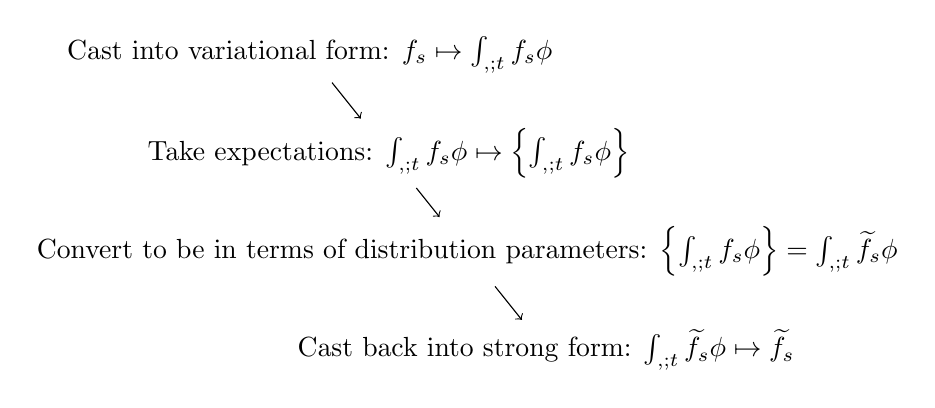
\begin{tikzpicture}[align = center, auto]
            \node (1) at (0, 0) {Cast into variational form: $f_{s}  \mapsto  \int_{\bfx, \bfv; t}f_{s}\phi$};
            \node (2) at (1, -1.25) {Take expectations: $\int_{\bfx, \bfv; t}f_{s}\phi  \mapsto  \bbE\left\{\int_{\bfx, \bfv; t}f_{s}\phi\right\}$};
            \node (3) at (2, -2.5) {Convert to be in terms of distribution parameters: $\bbE\left\{\int_{\bfx, \bfv; t}f_{s}\phi\right\}  =  \int_{\bfx, \bfv; t}\widetilde{f_{s}}\phi$};
            \node (4) at (3, -3.75) {Cast back into strong form: $\int_{\bfx, \bfv; t}\widetilde{f_{s}}\phi  \mapsto  \widetilde{f_{s}}$};

            \draw[->] (1) -- (2);
            \draw[->] (2) -- (3);
            \draw[->] (3) -- (4);
        \end{tikzpicture}
        \caption{Diagram of workflow for construction of a kinetic model}
        \label{fig:kinetic model construction workflow}
    \end{figure}

    \shortline

    \paragraph*{Maxwell's Equations} Since this process is entirely linear, Maxwell's equations---themselves linear---carry over identically:
    \begin{align}
        \frac{1}{\rmc^{2}}\partial_{t}\widetilde{\bfE}  &=  \nabla\wedge\widetilde{\bfB} - \mu_{0}\sum_{s}\rmq_{s}\int_{\bfv}\widetilde{f_{s}}\bfv,  &
        \partial_{t}\widetilde{\bfB}  &=  - \nabla\wedge\widetilde{\bfE},  \\
        \frac{1}{\rmc^{2}}\nabla\cdot\widetilde{\bfE}  &=  \mu_{0}\sum_{s}\rmq_{s}\int_{\bfv}\widetilde{f_{s}},  &
        \nabla\cdot\widetilde{\bfB}  &=  0.
    \end{align}
    where:
    \begin{itemize}
        \item  $\rmc$ is the speed of light (in a vacuum), $\rmc  \approx  2.997\ldots\times 10^{8}\rmm\rms^{- 1}$.
        \item  $\mu_{0}$ is the vacuum permeability, $\mu_{0}  \approx  1.257\ldots\times 10^{- 6}\rmT^{2}\rms^{2}\rmm^{1}{\rm kg}^{- 1}$.
    \end{itemize}
    \BA{I should probably initially define Maxwell's equations in the previous particle models subsection, instead of first here.}

    Defining the charge and current densities, $\rho_{\rmC}$ and $\bfj$ respectively, functions of $\bfx$ and $t$:
    \begin{align}
        \widetilde{\rho}_{\rmC}  :=  \int_{\bfv}\widetilde{f_{s}}\rmq_{s},  &&
               \widetilde{\bfj}  :=  \int_{\bfv}\widetilde{f_{s}}\rmq_{s}\bfv,
    \end{align}
    these can be written in the compact forms:
    \begin{align}
        \frac{1}{\rmc^{2}}\partial_{t}\widetilde{\bfE}  &=  \nabla\wedge\widetilde{\bfB} - \mu_{0}\widetilde{\bfj},  &
        \partial_{t}\widetilde{\bfB}  &=  - \nabla\wedge\widetilde{\bfE},  \label{eqn:Maxwell's equations transient}  \\
        \frac{1}{\rmc^{2}}\nabla\cdot\widetilde{\bfE}  &=  \mu_{0}\widetilde{\rho}_{\rmC},  &
        \nabla\cdot\widetilde{\bfB}  &=  0.  \label{eqn:Maxwell's equations steady-state}
    \end{align}
    
    \paragraph*{Boltzmann Equations} The evolution equations for $(f_{s})_{s}$ or $(\widetilde{f_{s}})_{s}$ are not as simple, due to their non-linearity. When applying this technique one derives the ``\emph{Boltzmann equations}'', \BA{[Ref]}
    \begin{equation}\label{eqn:Boltzmann equation}
        \partial_{t}\widetilde{f_{s}} + \nabla_{\bfx}\cdot\left[\widetilde{f_{s}}\bfv\right] + \frac{\rmq_{s}}{\rmm_{s}}\nabla_{\bfv}\cdot\left[\widetilde{f_{s}}\left(\widetilde{\bfE} + \bfv\wedge\widetilde{\bfB}\right)\right]  =   \frac{\rmq_{s}}{\rmm_{s}}\sum_{s'}\rmq_{s'}\nabla_{\bfv}\cdot\bfC_{ss'},
    \end{equation}
    where the collision terms $(\bfC_{ss'})_{ss'}$ are terms characterising the Coulomb collisions, defined as
    \begin{multline}\label{eqn:collision operator}
        \bfC_{ss'}\left[\widetilde{f_{s}}, \widetilde{f_{s'}}; \widetilde{f_{s}f_{s'}}\right](\bfx, \bfv; t)  :=  \int_{\bfx' \neq \bfx, \bfv'; t'}\left(\widetilde{f_{s}}(\bfx, \bfv; t)\widetilde{f_{s'}}(\bfx', \bfv'; t') - \widetilde{f_{s}f_{s'}}[(\bfx, \bfv; t), (\bfx', \bfv'; t')]\right)  \\
        [\bfk_{\bfE}(\bfx' - \bfx, \bfv'; t' - t) + \bfv\wedge\bfk_{\bfB}(\bfx' - \bfx, \bfv'; t' - t)],
    \end{multline}
    where in turn:
    \begin{itemize}
        \item  $\bfk_{\bfE}$, $\bfk_{\bfB}$, as functions in $\bfx'$, $\bfv'$, $t'$, are kernels of the electric and magnetic field, defined as the electric and magnetic fields produced at the origin by a unit point charge at position $\bfx'$ with velocity $\bfv'$ at time $t' \left(\in \left[-\frac{1}{c}\|\bfx'\|, 0\right]\right)$. \BA{(Explicit definition for $\bfk_{\bfE}$, $\bfk_{\bfB}$? Not really needed for the theory.)}
        
        \item  The 2-particle distributions functions $\left(\widetilde{f_{s_{1}}f_{s_{2}}}[(\bfx_{1}, \bfv_{1}; t_{1}), (\bfx_{2}, \bfv_{2}; t_{s})]\right)_{s_{1}s_{2}}$ are defined such that $\forall \phi[(\bfx_{1}, \bfv_{1}; t_{1}), (\bfx_{2}, \bfv_{2}; t_{2})]$,
        \begin{multline}
            \bbE\left\{\int_{\bfx_{1}, \bfv_{1}; t_{1}}\int_{\bfx_{2}, \bfv_{2}; t_{2}}f_{s_{1}}(\bfx_{1}, \bfv_{1}; t_{1})f_{s_{2}}(\bfx_{2}, \bfv_{2}; t_{2})\phi[(\bfx_{1}, \bfv_{1}; t_{1}), (\bfx_{2}, \bfv_{2}; t_{2})]\right\}  \\
            \left(=  \sum_{i_{1}, i_{2}}\bbE\{\phi[(\bfx_{s_{1}i_{1}}, \bfv_{s_{1}i_{1}}; t_{1}), (\bfx_{s_{2}i_{2}}, \bfv_{s_{2}i_{2}}; t_{2})]\}\right)  \\
            =  \int_{\bfx_{1}, \bfv_{1}}\int_{\bfx_{2}, \bfv_{2}}\widetilde{f_{s_{1}}f_{s_{2}}}[(\bfx_{1}, \bfv_{1}; t_{1}), (\bfx_{2}, \bfv_{2}; t_{2})]\phi[(\bfx_{1}, \bfv_{1}; t_{1}), (\bfx_{2}, \bfv_{2}; t_{2})].
        \end{multline}
        These capture some of the nature of how the positions of pairs of particles are correlated.
    \end{itemize}
    For a full derivation of (\ref{eqn:Boltzmann equation}) see Appendix \ref{cha:Boltzmann equation derivation}.

    Obviously this system is not closed, as it in turn is dependent on $\left(\widetilde{f_{s_{1}}f_{s_{2}}}\right)_{s_{1}s_{2}}$; this is referred to as the ``\emph{closure problem}''. Different approximations to $\left(\widetilde{f_{s_{1}}f_{s_{2}}}\right)_{s_{1}s_{2}}$ lead to different collisional forces and collision operators in the Boltzmann equation.

    \shortline

    From here, we shall drop the tildes $\widetilde{*}$ on $\widetilde{f_{s}}$, $\widetilde{\bfE}$, $\widetilde{\bfB}$, $\widetilde{\rho}_{\rmC}$, $\widetilde{\bfj}$, as we shall not be returning to the particle model. Together this system can be refered to as the Boltzmann--Maxwell system.


    \documentclass[12pt, a4paper]{report}

\documentclass[12pt, a4paper]{report}

\documentclass[12pt, a4paper]{report}

\input{template/main.tex}

\title{\BA{Title in Progress...}}
\author{Boris Andrews}
\affil{Mathematical Institute, University of Oxford}
\date{\today}


\begin{document}
    \pagenumbering{gobble}
    \maketitle
    
    
    \begin{abstract}
        Magnetic confinement reactors---in particular tokamaks---offer one of the most promising options for achieving practical nuclear fusion, with the potential to provide virtually limitless, clean energy. The theoretical and numerical modeling of tokamak plasmas is simultaneously an essential component of effective reactor design, and a great research barrier. Tokamak operational conditions exhibit comparatively low Knudsen numbers. Kinetic effects, including kinetic waves and instabilities, Landau damping, bump-on-tail instabilities and more, are therefore highly influential in tokamak plasma dynamics. Purely fluid models are inherently incapable of capturing these effects, whereas the high dimensionality in purely kinetic models render them practically intractable for most relevant purposes.

        We consider a $\delta\!f$ decomposition model, with a macroscopic fluid background and microscopic kinetic correction, both fully coupled to each other. A similar manner of discretization is proposed to that used in the recent \texttt{STRUPHY} code \cite{Holderied_Possanner_Wang_2021, Holderied_2022, Li_et_al_2023} with a finite-element model for the background and a pseudo-particle/PiC model for the correction.

        The fluid background satisfies the full, non-linear, resistive, compressible, Hall MHD equations. \cite{Laakmann_Hu_Farrell_2022} introduces finite-element(-in-space) implicit timesteppers for the incompressible analogue to this system with structure-preserving (SP) properties in the ideal case, alongside parameter-robust preconditioners. We show that these timesteppers can derive from a finite-element-in-time (FET) (and finite-element-in-space) interpretation. The benefits of this reformulation are discussed, including the derivation of timesteppers that are higher order in time, and the quantifiable dissipative SP properties in the non-ideal, resistive case.
        
        We discuss possible options for extending this FET approach to timesteppers for the compressible case.

        The kinetic corrections satisfy linearized Boltzmann equations. Using a Lénard--Bernstein collision operator, these take Fokker--Planck-like forms \cite{Fokker_1914, Planck_1917} wherein pseudo-particles in the numerical model obey the neoclassical transport equations, with particle-independent Brownian drift terms. This offers a rigorous methodology for incorporating collisions into the particle transport model, without coupling the equations of motions for each particle.
        
        Works by Chen, Chacón et al. \cite{Chen_Chacón_Barnes_2011, Chacón_Chen_Barnes_2013, Chen_Chacón_2014, Chen_Chacón_2015} have developed structure-preserving particle pushers for neoclassical transport in the Vlasov equations, derived from Crank--Nicolson integrators. We show these too can can derive from a FET interpretation, similarly offering potential extensions to higher-order-in-time particle pushers. The FET formulation is used also to consider how the stochastic drift terms can be incorporated into the pushers. Stochastic gyrokinetic expansions are also discussed.

        Different options for the numerical implementation of these schemes are considered.

        Due to the efficacy of FET in the development of SP timesteppers for both the fluid and kinetic component, we hope this approach will prove effective in the future for developing SP timesteppers for the full hybrid model. We hope this will give us the opportunity to incorporate previously inaccessible kinetic effects into the highly effective, modern, finite-element MHD models.
    \end{abstract}
    
    
    \newpage
    \tableofcontents
    
    
    \newpage
    \pagenumbering{arabic}
    %\linenumbers\renewcommand\thelinenumber{\color{black!50}\arabic{linenumber}}
            \input{0 - introduction/main.tex}
        \part{Research}
            \input{1 - low-noise PiC models/main.tex}
            \input{2 - kinetic component/main.tex}
            \input{3 - fluid component/main.tex}
            \input{4 - numerical implementation/main.tex}
        \part{Project Overview}
            \input{5 - research plan/main.tex}
            \input{6 - summary/main.tex}
    
    
    %\section{}
    \newpage
    \pagenumbering{gobble}
        \printbibliography


    \newpage
    \pagenumbering{roman}
    \appendix
        \part{Appendices}
            \input{8 - Hilbert complexes/main.tex}
            \input{9 - weak conservation proofs/main.tex}
\end{document}


\title{\BA{Title in Progress...}}
\author{Boris Andrews}
\affil{Mathematical Institute, University of Oxford}
\date{\today}


\begin{document}
    \pagenumbering{gobble}
    \maketitle
    
    
    \begin{abstract}
        Magnetic confinement reactors---in particular tokamaks---offer one of the most promising options for achieving practical nuclear fusion, with the potential to provide virtually limitless, clean energy. The theoretical and numerical modeling of tokamak plasmas is simultaneously an essential component of effective reactor design, and a great research barrier. Tokamak operational conditions exhibit comparatively low Knudsen numbers. Kinetic effects, including kinetic waves and instabilities, Landau damping, bump-on-tail instabilities and more, are therefore highly influential in tokamak plasma dynamics. Purely fluid models are inherently incapable of capturing these effects, whereas the high dimensionality in purely kinetic models render them practically intractable for most relevant purposes.

        We consider a $\delta\!f$ decomposition model, with a macroscopic fluid background and microscopic kinetic correction, both fully coupled to each other. A similar manner of discretization is proposed to that used in the recent \texttt{STRUPHY} code \cite{Holderied_Possanner_Wang_2021, Holderied_2022, Li_et_al_2023} with a finite-element model for the background and a pseudo-particle/PiC model for the correction.

        The fluid background satisfies the full, non-linear, resistive, compressible, Hall MHD equations. \cite{Laakmann_Hu_Farrell_2022} introduces finite-element(-in-space) implicit timesteppers for the incompressible analogue to this system with structure-preserving (SP) properties in the ideal case, alongside parameter-robust preconditioners. We show that these timesteppers can derive from a finite-element-in-time (FET) (and finite-element-in-space) interpretation. The benefits of this reformulation are discussed, including the derivation of timesteppers that are higher order in time, and the quantifiable dissipative SP properties in the non-ideal, resistive case.
        
        We discuss possible options for extending this FET approach to timesteppers for the compressible case.

        The kinetic corrections satisfy linearized Boltzmann equations. Using a Lénard--Bernstein collision operator, these take Fokker--Planck-like forms \cite{Fokker_1914, Planck_1917} wherein pseudo-particles in the numerical model obey the neoclassical transport equations, with particle-independent Brownian drift terms. This offers a rigorous methodology for incorporating collisions into the particle transport model, without coupling the equations of motions for each particle.
        
        Works by Chen, Chacón et al. \cite{Chen_Chacón_Barnes_2011, Chacón_Chen_Barnes_2013, Chen_Chacón_2014, Chen_Chacón_2015} have developed structure-preserving particle pushers for neoclassical transport in the Vlasov equations, derived from Crank--Nicolson integrators. We show these too can can derive from a FET interpretation, similarly offering potential extensions to higher-order-in-time particle pushers. The FET formulation is used also to consider how the stochastic drift terms can be incorporated into the pushers. Stochastic gyrokinetic expansions are also discussed.

        Different options for the numerical implementation of these schemes are considered.

        Due to the efficacy of FET in the development of SP timesteppers for both the fluid and kinetic component, we hope this approach will prove effective in the future for developing SP timesteppers for the full hybrid model. We hope this will give us the opportunity to incorporate previously inaccessible kinetic effects into the highly effective, modern, finite-element MHD models.
    \end{abstract}
    
    
    \newpage
    \tableofcontents
    
    
    \newpage
    \pagenumbering{arabic}
    %\linenumbers\renewcommand\thelinenumber{\color{black!50}\arabic{linenumber}}
            \documentclass[12pt, a4paper]{report}

\input{template/main.tex}

\title{\BA{Title in Progress...}}
\author{Boris Andrews}
\affil{Mathematical Institute, University of Oxford}
\date{\today}


\begin{document}
    \pagenumbering{gobble}
    \maketitle
    
    
    \begin{abstract}
        Magnetic confinement reactors---in particular tokamaks---offer one of the most promising options for achieving practical nuclear fusion, with the potential to provide virtually limitless, clean energy. The theoretical and numerical modeling of tokamak plasmas is simultaneously an essential component of effective reactor design, and a great research barrier. Tokamak operational conditions exhibit comparatively low Knudsen numbers. Kinetic effects, including kinetic waves and instabilities, Landau damping, bump-on-tail instabilities and more, are therefore highly influential in tokamak plasma dynamics. Purely fluid models are inherently incapable of capturing these effects, whereas the high dimensionality in purely kinetic models render them practically intractable for most relevant purposes.

        We consider a $\delta\!f$ decomposition model, with a macroscopic fluid background and microscopic kinetic correction, both fully coupled to each other. A similar manner of discretization is proposed to that used in the recent \texttt{STRUPHY} code \cite{Holderied_Possanner_Wang_2021, Holderied_2022, Li_et_al_2023} with a finite-element model for the background and a pseudo-particle/PiC model for the correction.

        The fluid background satisfies the full, non-linear, resistive, compressible, Hall MHD equations. \cite{Laakmann_Hu_Farrell_2022} introduces finite-element(-in-space) implicit timesteppers for the incompressible analogue to this system with structure-preserving (SP) properties in the ideal case, alongside parameter-robust preconditioners. We show that these timesteppers can derive from a finite-element-in-time (FET) (and finite-element-in-space) interpretation. The benefits of this reformulation are discussed, including the derivation of timesteppers that are higher order in time, and the quantifiable dissipative SP properties in the non-ideal, resistive case.
        
        We discuss possible options for extending this FET approach to timesteppers for the compressible case.

        The kinetic corrections satisfy linearized Boltzmann equations. Using a Lénard--Bernstein collision operator, these take Fokker--Planck-like forms \cite{Fokker_1914, Planck_1917} wherein pseudo-particles in the numerical model obey the neoclassical transport equations, with particle-independent Brownian drift terms. This offers a rigorous methodology for incorporating collisions into the particle transport model, without coupling the equations of motions for each particle.
        
        Works by Chen, Chacón et al. \cite{Chen_Chacón_Barnes_2011, Chacón_Chen_Barnes_2013, Chen_Chacón_2014, Chen_Chacón_2015} have developed structure-preserving particle pushers for neoclassical transport in the Vlasov equations, derived from Crank--Nicolson integrators. We show these too can can derive from a FET interpretation, similarly offering potential extensions to higher-order-in-time particle pushers. The FET formulation is used also to consider how the stochastic drift terms can be incorporated into the pushers. Stochastic gyrokinetic expansions are also discussed.

        Different options for the numerical implementation of these schemes are considered.

        Due to the efficacy of FET in the development of SP timesteppers for both the fluid and kinetic component, we hope this approach will prove effective in the future for developing SP timesteppers for the full hybrid model. We hope this will give us the opportunity to incorporate previously inaccessible kinetic effects into the highly effective, modern, finite-element MHD models.
    \end{abstract}
    
    
    \newpage
    \tableofcontents
    
    
    \newpage
    \pagenumbering{arabic}
    %\linenumbers\renewcommand\thelinenumber{\color{black!50}\arabic{linenumber}}
            \input{0 - introduction/main.tex}
        \part{Research}
            \input{1 - low-noise PiC models/main.tex}
            \input{2 - kinetic component/main.tex}
            \input{3 - fluid component/main.tex}
            \input{4 - numerical implementation/main.tex}
        \part{Project Overview}
            \input{5 - research plan/main.tex}
            \input{6 - summary/main.tex}
    
    
    %\section{}
    \newpage
    \pagenumbering{gobble}
        \printbibliography


    \newpage
    \pagenumbering{roman}
    \appendix
        \part{Appendices}
            \input{8 - Hilbert complexes/main.tex}
            \input{9 - weak conservation proofs/main.tex}
\end{document}

        \part{Research}
            \documentclass[12pt, a4paper]{report}

\input{template/main.tex}

\title{\BA{Title in Progress...}}
\author{Boris Andrews}
\affil{Mathematical Institute, University of Oxford}
\date{\today}


\begin{document}
    \pagenumbering{gobble}
    \maketitle
    
    
    \begin{abstract}
        Magnetic confinement reactors---in particular tokamaks---offer one of the most promising options for achieving practical nuclear fusion, with the potential to provide virtually limitless, clean energy. The theoretical and numerical modeling of tokamak plasmas is simultaneously an essential component of effective reactor design, and a great research barrier. Tokamak operational conditions exhibit comparatively low Knudsen numbers. Kinetic effects, including kinetic waves and instabilities, Landau damping, bump-on-tail instabilities and more, are therefore highly influential in tokamak plasma dynamics. Purely fluid models are inherently incapable of capturing these effects, whereas the high dimensionality in purely kinetic models render them practically intractable for most relevant purposes.

        We consider a $\delta\!f$ decomposition model, with a macroscopic fluid background and microscopic kinetic correction, both fully coupled to each other. A similar manner of discretization is proposed to that used in the recent \texttt{STRUPHY} code \cite{Holderied_Possanner_Wang_2021, Holderied_2022, Li_et_al_2023} with a finite-element model for the background and a pseudo-particle/PiC model for the correction.

        The fluid background satisfies the full, non-linear, resistive, compressible, Hall MHD equations. \cite{Laakmann_Hu_Farrell_2022} introduces finite-element(-in-space) implicit timesteppers for the incompressible analogue to this system with structure-preserving (SP) properties in the ideal case, alongside parameter-robust preconditioners. We show that these timesteppers can derive from a finite-element-in-time (FET) (and finite-element-in-space) interpretation. The benefits of this reformulation are discussed, including the derivation of timesteppers that are higher order in time, and the quantifiable dissipative SP properties in the non-ideal, resistive case.
        
        We discuss possible options for extending this FET approach to timesteppers for the compressible case.

        The kinetic corrections satisfy linearized Boltzmann equations. Using a Lénard--Bernstein collision operator, these take Fokker--Planck-like forms \cite{Fokker_1914, Planck_1917} wherein pseudo-particles in the numerical model obey the neoclassical transport equations, with particle-independent Brownian drift terms. This offers a rigorous methodology for incorporating collisions into the particle transport model, without coupling the equations of motions for each particle.
        
        Works by Chen, Chacón et al. \cite{Chen_Chacón_Barnes_2011, Chacón_Chen_Barnes_2013, Chen_Chacón_2014, Chen_Chacón_2015} have developed structure-preserving particle pushers for neoclassical transport in the Vlasov equations, derived from Crank--Nicolson integrators. We show these too can can derive from a FET interpretation, similarly offering potential extensions to higher-order-in-time particle pushers. The FET formulation is used also to consider how the stochastic drift terms can be incorporated into the pushers. Stochastic gyrokinetic expansions are also discussed.

        Different options for the numerical implementation of these schemes are considered.

        Due to the efficacy of FET in the development of SP timesteppers for both the fluid and kinetic component, we hope this approach will prove effective in the future for developing SP timesteppers for the full hybrid model. We hope this will give us the opportunity to incorporate previously inaccessible kinetic effects into the highly effective, modern, finite-element MHD models.
    \end{abstract}
    
    
    \newpage
    \tableofcontents
    
    
    \newpage
    \pagenumbering{arabic}
    %\linenumbers\renewcommand\thelinenumber{\color{black!50}\arabic{linenumber}}
            \input{0 - introduction/main.tex}
        \part{Research}
            \input{1 - low-noise PiC models/main.tex}
            \input{2 - kinetic component/main.tex}
            \input{3 - fluid component/main.tex}
            \input{4 - numerical implementation/main.tex}
        \part{Project Overview}
            \input{5 - research plan/main.tex}
            \input{6 - summary/main.tex}
    
    
    %\section{}
    \newpage
    \pagenumbering{gobble}
        \printbibliography


    \newpage
    \pagenumbering{roman}
    \appendix
        \part{Appendices}
            \input{8 - Hilbert complexes/main.tex}
            \input{9 - weak conservation proofs/main.tex}
\end{document}

            \documentclass[12pt, a4paper]{report}

\input{template/main.tex}

\title{\BA{Title in Progress...}}
\author{Boris Andrews}
\affil{Mathematical Institute, University of Oxford}
\date{\today}


\begin{document}
    \pagenumbering{gobble}
    \maketitle
    
    
    \begin{abstract}
        Magnetic confinement reactors---in particular tokamaks---offer one of the most promising options for achieving practical nuclear fusion, with the potential to provide virtually limitless, clean energy. The theoretical and numerical modeling of tokamak plasmas is simultaneously an essential component of effective reactor design, and a great research barrier. Tokamak operational conditions exhibit comparatively low Knudsen numbers. Kinetic effects, including kinetic waves and instabilities, Landau damping, bump-on-tail instabilities and more, are therefore highly influential in tokamak plasma dynamics. Purely fluid models are inherently incapable of capturing these effects, whereas the high dimensionality in purely kinetic models render them practically intractable for most relevant purposes.

        We consider a $\delta\!f$ decomposition model, with a macroscopic fluid background and microscopic kinetic correction, both fully coupled to each other. A similar manner of discretization is proposed to that used in the recent \texttt{STRUPHY} code \cite{Holderied_Possanner_Wang_2021, Holderied_2022, Li_et_al_2023} with a finite-element model for the background and a pseudo-particle/PiC model for the correction.

        The fluid background satisfies the full, non-linear, resistive, compressible, Hall MHD equations. \cite{Laakmann_Hu_Farrell_2022} introduces finite-element(-in-space) implicit timesteppers for the incompressible analogue to this system with structure-preserving (SP) properties in the ideal case, alongside parameter-robust preconditioners. We show that these timesteppers can derive from a finite-element-in-time (FET) (and finite-element-in-space) interpretation. The benefits of this reformulation are discussed, including the derivation of timesteppers that are higher order in time, and the quantifiable dissipative SP properties in the non-ideal, resistive case.
        
        We discuss possible options for extending this FET approach to timesteppers for the compressible case.

        The kinetic corrections satisfy linearized Boltzmann equations. Using a Lénard--Bernstein collision operator, these take Fokker--Planck-like forms \cite{Fokker_1914, Planck_1917} wherein pseudo-particles in the numerical model obey the neoclassical transport equations, with particle-independent Brownian drift terms. This offers a rigorous methodology for incorporating collisions into the particle transport model, without coupling the equations of motions for each particle.
        
        Works by Chen, Chacón et al. \cite{Chen_Chacón_Barnes_2011, Chacón_Chen_Barnes_2013, Chen_Chacón_2014, Chen_Chacón_2015} have developed structure-preserving particle pushers for neoclassical transport in the Vlasov equations, derived from Crank--Nicolson integrators. We show these too can can derive from a FET interpretation, similarly offering potential extensions to higher-order-in-time particle pushers. The FET formulation is used also to consider how the stochastic drift terms can be incorporated into the pushers. Stochastic gyrokinetic expansions are also discussed.

        Different options for the numerical implementation of these schemes are considered.

        Due to the efficacy of FET in the development of SP timesteppers for both the fluid and kinetic component, we hope this approach will prove effective in the future for developing SP timesteppers for the full hybrid model. We hope this will give us the opportunity to incorporate previously inaccessible kinetic effects into the highly effective, modern, finite-element MHD models.
    \end{abstract}
    
    
    \newpage
    \tableofcontents
    
    
    \newpage
    \pagenumbering{arabic}
    %\linenumbers\renewcommand\thelinenumber{\color{black!50}\arabic{linenumber}}
            \input{0 - introduction/main.tex}
        \part{Research}
            \input{1 - low-noise PiC models/main.tex}
            \input{2 - kinetic component/main.tex}
            \input{3 - fluid component/main.tex}
            \input{4 - numerical implementation/main.tex}
        \part{Project Overview}
            \input{5 - research plan/main.tex}
            \input{6 - summary/main.tex}
    
    
    %\section{}
    \newpage
    \pagenumbering{gobble}
        \printbibliography


    \newpage
    \pagenumbering{roman}
    \appendix
        \part{Appendices}
            \input{8 - Hilbert complexes/main.tex}
            \input{9 - weak conservation proofs/main.tex}
\end{document}

            \documentclass[12pt, a4paper]{report}

\input{template/main.tex}

\title{\BA{Title in Progress...}}
\author{Boris Andrews}
\affil{Mathematical Institute, University of Oxford}
\date{\today}


\begin{document}
    \pagenumbering{gobble}
    \maketitle
    
    
    \begin{abstract}
        Magnetic confinement reactors---in particular tokamaks---offer one of the most promising options for achieving practical nuclear fusion, with the potential to provide virtually limitless, clean energy. The theoretical and numerical modeling of tokamak plasmas is simultaneously an essential component of effective reactor design, and a great research barrier. Tokamak operational conditions exhibit comparatively low Knudsen numbers. Kinetic effects, including kinetic waves and instabilities, Landau damping, bump-on-tail instabilities and more, are therefore highly influential in tokamak plasma dynamics. Purely fluid models are inherently incapable of capturing these effects, whereas the high dimensionality in purely kinetic models render them practically intractable for most relevant purposes.

        We consider a $\delta\!f$ decomposition model, with a macroscopic fluid background and microscopic kinetic correction, both fully coupled to each other. A similar manner of discretization is proposed to that used in the recent \texttt{STRUPHY} code \cite{Holderied_Possanner_Wang_2021, Holderied_2022, Li_et_al_2023} with a finite-element model for the background and a pseudo-particle/PiC model for the correction.

        The fluid background satisfies the full, non-linear, resistive, compressible, Hall MHD equations. \cite{Laakmann_Hu_Farrell_2022} introduces finite-element(-in-space) implicit timesteppers for the incompressible analogue to this system with structure-preserving (SP) properties in the ideal case, alongside parameter-robust preconditioners. We show that these timesteppers can derive from a finite-element-in-time (FET) (and finite-element-in-space) interpretation. The benefits of this reformulation are discussed, including the derivation of timesteppers that are higher order in time, and the quantifiable dissipative SP properties in the non-ideal, resistive case.
        
        We discuss possible options for extending this FET approach to timesteppers for the compressible case.

        The kinetic corrections satisfy linearized Boltzmann equations. Using a Lénard--Bernstein collision operator, these take Fokker--Planck-like forms \cite{Fokker_1914, Planck_1917} wherein pseudo-particles in the numerical model obey the neoclassical transport equations, with particle-independent Brownian drift terms. This offers a rigorous methodology for incorporating collisions into the particle transport model, without coupling the equations of motions for each particle.
        
        Works by Chen, Chacón et al. \cite{Chen_Chacón_Barnes_2011, Chacón_Chen_Barnes_2013, Chen_Chacón_2014, Chen_Chacón_2015} have developed structure-preserving particle pushers for neoclassical transport in the Vlasov equations, derived from Crank--Nicolson integrators. We show these too can can derive from a FET interpretation, similarly offering potential extensions to higher-order-in-time particle pushers. The FET formulation is used also to consider how the stochastic drift terms can be incorporated into the pushers. Stochastic gyrokinetic expansions are also discussed.

        Different options for the numerical implementation of these schemes are considered.

        Due to the efficacy of FET in the development of SP timesteppers for both the fluid and kinetic component, we hope this approach will prove effective in the future for developing SP timesteppers for the full hybrid model. We hope this will give us the opportunity to incorporate previously inaccessible kinetic effects into the highly effective, modern, finite-element MHD models.
    \end{abstract}
    
    
    \newpage
    \tableofcontents
    
    
    \newpage
    \pagenumbering{arabic}
    %\linenumbers\renewcommand\thelinenumber{\color{black!50}\arabic{linenumber}}
            \input{0 - introduction/main.tex}
        \part{Research}
            \input{1 - low-noise PiC models/main.tex}
            \input{2 - kinetic component/main.tex}
            \input{3 - fluid component/main.tex}
            \input{4 - numerical implementation/main.tex}
        \part{Project Overview}
            \input{5 - research plan/main.tex}
            \input{6 - summary/main.tex}
    
    
    %\section{}
    \newpage
    \pagenumbering{gobble}
        \printbibliography


    \newpage
    \pagenumbering{roman}
    \appendix
        \part{Appendices}
            \input{8 - Hilbert complexes/main.tex}
            \input{9 - weak conservation proofs/main.tex}
\end{document}

            \documentclass[12pt, a4paper]{report}

\input{template/main.tex}

\title{\BA{Title in Progress...}}
\author{Boris Andrews}
\affil{Mathematical Institute, University of Oxford}
\date{\today}


\begin{document}
    \pagenumbering{gobble}
    \maketitle
    
    
    \begin{abstract}
        Magnetic confinement reactors---in particular tokamaks---offer one of the most promising options for achieving practical nuclear fusion, with the potential to provide virtually limitless, clean energy. The theoretical and numerical modeling of tokamak plasmas is simultaneously an essential component of effective reactor design, and a great research barrier. Tokamak operational conditions exhibit comparatively low Knudsen numbers. Kinetic effects, including kinetic waves and instabilities, Landau damping, bump-on-tail instabilities and more, are therefore highly influential in tokamak plasma dynamics. Purely fluid models are inherently incapable of capturing these effects, whereas the high dimensionality in purely kinetic models render them practically intractable for most relevant purposes.

        We consider a $\delta\!f$ decomposition model, with a macroscopic fluid background and microscopic kinetic correction, both fully coupled to each other. A similar manner of discretization is proposed to that used in the recent \texttt{STRUPHY} code \cite{Holderied_Possanner_Wang_2021, Holderied_2022, Li_et_al_2023} with a finite-element model for the background and a pseudo-particle/PiC model for the correction.

        The fluid background satisfies the full, non-linear, resistive, compressible, Hall MHD equations. \cite{Laakmann_Hu_Farrell_2022} introduces finite-element(-in-space) implicit timesteppers for the incompressible analogue to this system with structure-preserving (SP) properties in the ideal case, alongside parameter-robust preconditioners. We show that these timesteppers can derive from a finite-element-in-time (FET) (and finite-element-in-space) interpretation. The benefits of this reformulation are discussed, including the derivation of timesteppers that are higher order in time, and the quantifiable dissipative SP properties in the non-ideal, resistive case.
        
        We discuss possible options for extending this FET approach to timesteppers for the compressible case.

        The kinetic corrections satisfy linearized Boltzmann equations. Using a Lénard--Bernstein collision operator, these take Fokker--Planck-like forms \cite{Fokker_1914, Planck_1917} wherein pseudo-particles in the numerical model obey the neoclassical transport equations, with particle-independent Brownian drift terms. This offers a rigorous methodology for incorporating collisions into the particle transport model, without coupling the equations of motions for each particle.
        
        Works by Chen, Chacón et al. \cite{Chen_Chacón_Barnes_2011, Chacón_Chen_Barnes_2013, Chen_Chacón_2014, Chen_Chacón_2015} have developed structure-preserving particle pushers for neoclassical transport in the Vlasov equations, derived from Crank--Nicolson integrators. We show these too can can derive from a FET interpretation, similarly offering potential extensions to higher-order-in-time particle pushers. The FET formulation is used also to consider how the stochastic drift terms can be incorporated into the pushers. Stochastic gyrokinetic expansions are also discussed.

        Different options for the numerical implementation of these schemes are considered.

        Due to the efficacy of FET in the development of SP timesteppers for both the fluid and kinetic component, we hope this approach will prove effective in the future for developing SP timesteppers for the full hybrid model. We hope this will give us the opportunity to incorporate previously inaccessible kinetic effects into the highly effective, modern, finite-element MHD models.
    \end{abstract}
    
    
    \newpage
    \tableofcontents
    
    
    \newpage
    \pagenumbering{arabic}
    %\linenumbers\renewcommand\thelinenumber{\color{black!50}\arabic{linenumber}}
            \input{0 - introduction/main.tex}
        \part{Research}
            \input{1 - low-noise PiC models/main.tex}
            \input{2 - kinetic component/main.tex}
            \input{3 - fluid component/main.tex}
            \input{4 - numerical implementation/main.tex}
        \part{Project Overview}
            \input{5 - research plan/main.tex}
            \input{6 - summary/main.tex}
    
    
    %\section{}
    \newpage
    \pagenumbering{gobble}
        \printbibliography


    \newpage
    \pagenumbering{roman}
    \appendix
        \part{Appendices}
            \input{8 - Hilbert complexes/main.tex}
            \input{9 - weak conservation proofs/main.tex}
\end{document}

        \part{Project Overview}
            \documentclass[12pt, a4paper]{report}

\input{template/main.tex}

\title{\BA{Title in Progress...}}
\author{Boris Andrews}
\affil{Mathematical Institute, University of Oxford}
\date{\today}


\begin{document}
    \pagenumbering{gobble}
    \maketitle
    
    
    \begin{abstract}
        Magnetic confinement reactors---in particular tokamaks---offer one of the most promising options for achieving practical nuclear fusion, with the potential to provide virtually limitless, clean energy. The theoretical and numerical modeling of tokamak plasmas is simultaneously an essential component of effective reactor design, and a great research barrier. Tokamak operational conditions exhibit comparatively low Knudsen numbers. Kinetic effects, including kinetic waves and instabilities, Landau damping, bump-on-tail instabilities and more, are therefore highly influential in tokamak plasma dynamics. Purely fluid models are inherently incapable of capturing these effects, whereas the high dimensionality in purely kinetic models render them practically intractable for most relevant purposes.

        We consider a $\delta\!f$ decomposition model, with a macroscopic fluid background and microscopic kinetic correction, both fully coupled to each other. A similar manner of discretization is proposed to that used in the recent \texttt{STRUPHY} code \cite{Holderied_Possanner_Wang_2021, Holderied_2022, Li_et_al_2023} with a finite-element model for the background and a pseudo-particle/PiC model for the correction.

        The fluid background satisfies the full, non-linear, resistive, compressible, Hall MHD equations. \cite{Laakmann_Hu_Farrell_2022} introduces finite-element(-in-space) implicit timesteppers for the incompressible analogue to this system with structure-preserving (SP) properties in the ideal case, alongside parameter-robust preconditioners. We show that these timesteppers can derive from a finite-element-in-time (FET) (and finite-element-in-space) interpretation. The benefits of this reformulation are discussed, including the derivation of timesteppers that are higher order in time, and the quantifiable dissipative SP properties in the non-ideal, resistive case.
        
        We discuss possible options for extending this FET approach to timesteppers for the compressible case.

        The kinetic corrections satisfy linearized Boltzmann equations. Using a Lénard--Bernstein collision operator, these take Fokker--Planck-like forms \cite{Fokker_1914, Planck_1917} wherein pseudo-particles in the numerical model obey the neoclassical transport equations, with particle-independent Brownian drift terms. This offers a rigorous methodology for incorporating collisions into the particle transport model, without coupling the equations of motions for each particle.
        
        Works by Chen, Chacón et al. \cite{Chen_Chacón_Barnes_2011, Chacón_Chen_Barnes_2013, Chen_Chacón_2014, Chen_Chacón_2015} have developed structure-preserving particle pushers for neoclassical transport in the Vlasov equations, derived from Crank--Nicolson integrators. We show these too can can derive from a FET interpretation, similarly offering potential extensions to higher-order-in-time particle pushers. The FET formulation is used also to consider how the stochastic drift terms can be incorporated into the pushers. Stochastic gyrokinetic expansions are also discussed.

        Different options for the numerical implementation of these schemes are considered.

        Due to the efficacy of FET in the development of SP timesteppers for both the fluid and kinetic component, we hope this approach will prove effective in the future for developing SP timesteppers for the full hybrid model. We hope this will give us the opportunity to incorporate previously inaccessible kinetic effects into the highly effective, modern, finite-element MHD models.
    \end{abstract}
    
    
    \newpage
    \tableofcontents
    
    
    \newpage
    \pagenumbering{arabic}
    %\linenumbers\renewcommand\thelinenumber{\color{black!50}\arabic{linenumber}}
            \input{0 - introduction/main.tex}
        \part{Research}
            \input{1 - low-noise PiC models/main.tex}
            \input{2 - kinetic component/main.tex}
            \input{3 - fluid component/main.tex}
            \input{4 - numerical implementation/main.tex}
        \part{Project Overview}
            \input{5 - research plan/main.tex}
            \input{6 - summary/main.tex}
    
    
    %\section{}
    \newpage
    \pagenumbering{gobble}
        \printbibliography


    \newpage
    \pagenumbering{roman}
    \appendix
        \part{Appendices}
            \input{8 - Hilbert complexes/main.tex}
            \input{9 - weak conservation proofs/main.tex}
\end{document}

            \documentclass[12pt, a4paper]{report}

\input{template/main.tex}

\title{\BA{Title in Progress...}}
\author{Boris Andrews}
\affil{Mathematical Institute, University of Oxford}
\date{\today}


\begin{document}
    \pagenumbering{gobble}
    \maketitle
    
    
    \begin{abstract}
        Magnetic confinement reactors---in particular tokamaks---offer one of the most promising options for achieving practical nuclear fusion, with the potential to provide virtually limitless, clean energy. The theoretical and numerical modeling of tokamak plasmas is simultaneously an essential component of effective reactor design, and a great research barrier. Tokamak operational conditions exhibit comparatively low Knudsen numbers. Kinetic effects, including kinetic waves and instabilities, Landau damping, bump-on-tail instabilities and more, are therefore highly influential in tokamak plasma dynamics. Purely fluid models are inherently incapable of capturing these effects, whereas the high dimensionality in purely kinetic models render them practically intractable for most relevant purposes.

        We consider a $\delta\!f$ decomposition model, with a macroscopic fluid background and microscopic kinetic correction, both fully coupled to each other. A similar manner of discretization is proposed to that used in the recent \texttt{STRUPHY} code \cite{Holderied_Possanner_Wang_2021, Holderied_2022, Li_et_al_2023} with a finite-element model for the background and a pseudo-particle/PiC model for the correction.

        The fluid background satisfies the full, non-linear, resistive, compressible, Hall MHD equations. \cite{Laakmann_Hu_Farrell_2022} introduces finite-element(-in-space) implicit timesteppers for the incompressible analogue to this system with structure-preserving (SP) properties in the ideal case, alongside parameter-robust preconditioners. We show that these timesteppers can derive from a finite-element-in-time (FET) (and finite-element-in-space) interpretation. The benefits of this reformulation are discussed, including the derivation of timesteppers that are higher order in time, and the quantifiable dissipative SP properties in the non-ideal, resistive case.
        
        We discuss possible options for extending this FET approach to timesteppers for the compressible case.

        The kinetic corrections satisfy linearized Boltzmann equations. Using a Lénard--Bernstein collision operator, these take Fokker--Planck-like forms \cite{Fokker_1914, Planck_1917} wherein pseudo-particles in the numerical model obey the neoclassical transport equations, with particle-independent Brownian drift terms. This offers a rigorous methodology for incorporating collisions into the particle transport model, without coupling the equations of motions for each particle.
        
        Works by Chen, Chacón et al. \cite{Chen_Chacón_Barnes_2011, Chacón_Chen_Barnes_2013, Chen_Chacón_2014, Chen_Chacón_2015} have developed structure-preserving particle pushers for neoclassical transport in the Vlasov equations, derived from Crank--Nicolson integrators. We show these too can can derive from a FET interpretation, similarly offering potential extensions to higher-order-in-time particle pushers. The FET formulation is used also to consider how the stochastic drift terms can be incorporated into the pushers. Stochastic gyrokinetic expansions are also discussed.

        Different options for the numerical implementation of these schemes are considered.

        Due to the efficacy of FET in the development of SP timesteppers for both the fluid and kinetic component, we hope this approach will prove effective in the future for developing SP timesteppers for the full hybrid model. We hope this will give us the opportunity to incorporate previously inaccessible kinetic effects into the highly effective, modern, finite-element MHD models.
    \end{abstract}
    
    
    \newpage
    \tableofcontents
    
    
    \newpage
    \pagenumbering{arabic}
    %\linenumbers\renewcommand\thelinenumber{\color{black!50}\arabic{linenumber}}
            \input{0 - introduction/main.tex}
        \part{Research}
            \input{1 - low-noise PiC models/main.tex}
            \input{2 - kinetic component/main.tex}
            \input{3 - fluid component/main.tex}
            \input{4 - numerical implementation/main.tex}
        \part{Project Overview}
            \input{5 - research plan/main.tex}
            \input{6 - summary/main.tex}
    
    
    %\section{}
    \newpage
    \pagenumbering{gobble}
        \printbibliography


    \newpage
    \pagenumbering{roman}
    \appendix
        \part{Appendices}
            \input{8 - Hilbert complexes/main.tex}
            \input{9 - weak conservation proofs/main.tex}
\end{document}

    
    
    %\section{}
    \newpage
    \pagenumbering{gobble}
        \printbibliography


    \newpage
    \pagenumbering{roman}
    \appendix
        \part{Appendices}
            \documentclass[12pt, a4paper]{report}

\input{template/main.tex}

\title{\BA{Title in Progress...}}
\author{Boris Andrews}
\affil{Mathematical Institute, University of Oxford}
\date{\today}


\begin{document}
    \pagenumbering{gobble}
    \maketitle
    
    
    \begin{abstract}
        Magnetic confinement reactors---in particular tokamaks---offer one of the most promising options for achieving practical nuclear fusion, with the potential to provide virtually limitless, clean energy. The theoretical and numerical modeling of tokamak plasmas is simultaneously an essential component of effective reactor design, and a great research barrier. Tokamak operational conditions exhibit comparatively low Knudsen numbers. Kinetic effects, including kinetic waves and instabilities, Landau damping, bump-on-tail instabilities and more, are therefore highly influential in tokamak plasma dynamics. Purely fluid models are inherently incapable of capturing these effects, whereas the high dimensionality in purely kinetic models render them practically intractable for most relevant purposes.

        We consider a $\delta\!f$ decomposition model, with a macroscopic fluid background and microscopic kinetic correction, both fully coupled to each other. A similar manner of discretization is proposed to that used in the recent \texttt{STRUPHY} code \cite{Holderied_Possanner_Wang_2021, Holderied_2022, Li_et_al_2023} with a finite-element model for the background and a pseudo-particle/PiC model for the correction.

        The fluid background satisfies the full, non-linear, resistive, compressible, Hall MHD equations. \cite{Laakmann_Hu_Farrell_2022} introduces finite-element(-in-space) implicit timesteppers for the incompressible analogue to this system with structure-preserving (SP) properties in the ideal case, alongside parameter-robust preconditioners. We show that these timesteppers can derive from a finite-element-in-time (FET) (and finite-element-in-space) interpretation. The benefits of this reformulation are discussed, including the derivation of timesteppers that are higher order in time, and the quantifiable dissipative SP properties in the non-ideal, resistive case.
        
        We discuss possible options for extending this FET approach to timesteppers for the compressible case.

        The kinetic corrections satisfy linearized Boltzmann equations. Using a Lénard--Bernstein collision operator, these take Fokker--Planck-like forms \cite{Fokker_1914, Planck_1917} wherein pseudo-particles in the numerical model obey the neoclassical transport equations, with particle-independent Brownian drift terms. This offers a rigorous methodology for incorporating collisions into the particle transport model, without coupling the equations of motions for each particle.
        
        Works by Chen, Chacón et al. \cite{Chen_Chacón_Barnes_2011, Chacón_Chen_Barnes_2013, Chen_Chacón_2014, Chen_Chacón_2015} have developed structure-preserving particle pushers for neoclassical transport in the Vlasov equations, derived from Crank--Nicolson integrators. We show these too can can derive from a FET interpretation, similarly offering potential extensions to higher-order-in-time particle pushers. The FET formulation is used also to consider how the stochastic drift terms can be incorporated into the pushers. Stochastic gyrokinetic expansions are also discussed.

        Different options for the numerical implementation of these schemes are considered.

        Due to the efficacy of FET in the development of SP timesteppers for both the fluid and kinetic component, we hope this approach will prove effective in the future for developing SP timesteppers for the full hybrid model. We hope this will give us the opportunity to incorporate previously inaccessible kinetic effects into the highly effective, modern, finite-element MHD models.
    \end{abstract}
    
    
    \newpage
    \tableofcontents
    
    
    \newpage
    \pagenumbering{arabic}
    %\linenumbers\renewcommand\thelinenumber{\color{black!50}\arabic{linenumber}}
            \input{0 - introduction/main.tex}
        \part{Research}
            \input{1 - low-noise PiC models/main.tex}
            \input{2 - kinetic component/main.tex}
            \input{3 - fluid component/main.tex}
            \input{4 - numerical implementation/main.tex}
        \part{Project Overview}
            \input{5 - research plan/main.tex}
            \input{6 - summary/main.tex}
    
    
    %\section{}
    \newpage
    \pagenumbering{gobble}
        \printbibliography


    \newpage
    \pagenumbering{roman}
    \appendix
        \part{Appendices}
            \input{8 - Hilbert complexes/main.tex}
            \input{9 - weak conservation proofs/main.tex}
\end{document}

            \documentclass[12pt, a4paper]{report}

\input{template/main.tex}

\title{\BA{Title in Progress...}}
\author{Boris Andrews}
\affil{Mathematical Institute, University of Oxford}
\date{\today}


\begin{document}
    \pagenumbering{gobble}
    \maketitle
    
    
    \begin{abstract}
        Magnetic confinement reactors---in particular tokamaks---offer one of the most promising options for achieving practical nuclear fusion, with the potential to provide virtually limitless, clean energy. The theoretical and numerical modeling of tokamak plasmas is simultaneously an essential component of effective reactor design, and a great research barrier. Tokamak operational conditions exhibit comparatively low Knudsen numbers. Kinetic effects, including kinetic waves and instabilities, Landau damping, bump-on-tail instabilities and more, are therefore highly influential in tokamak plasma dynamics. Purely fluid models are inherently incapable of capturing these effects, whereas the high dimensionality in purely kinetic models render them practically intractable for most relevant purposes.

        We consider a $\delta\!f$ decomposition model, with a macroscopic fluid background and microscopic kinetic correction, both fully coupled to each other. A similar manner of discretization is proposed to that used in the recent \texttt{STRUPHY} code \cite{Holderied_Possanner_Wang_2021, Holderied_2022, Li_et_al_2023} with a finite-element model for the background and a pseudo-particle/PiC model for the correction.

        The fluid background satisfies the full, non-linear, resistive, compressible, Hall MHD equations. \cite{Laakmann_Hu_Farrell_2022} introduces finite-element(-in-space) implicit timesteppers for the incompressible analogue to this system with structure-preserving (SP) properties in the ideal case, alongside parameter-robust preconditioners. We show that these timesteppers can derive from a finite-element-in-time (FET) (and finite-element-in-space) interpretation. The benefits of this reformulation are discussed, including the derivation of timesteppers that are higher order in time, and the quantifiable dissipative SP properties in the non-ideal, resistive case.
        
        We discuss possible options for extending this FET approach to timesteppers for the compressible case.

        The kinetic corrections satisfy linearized Boltzmann equations. Using a Lénard--Bernstein collision operator, these take Fokker--Planck-like forms \cite{Fokker_1914, Planck_1917} wherein pseudo-particles in the numerical model obey the neoclassical transport equations, with particle-independent Brownian drift terms. This offers a rigorous methodology for incorporating collisions into the particle transport model, without coupling the equations of motions for each particle.
        
        Works by Chen, Chacón et al. \cite{Chen_Chacón_Barnes_2011, Chacón_Chen_Barnes_2013, Chen_Chacón_2014, Chen_Chacón_2015} have developed structure-preserving particle pushers for neoclassical transport in the Vlasov equations, derived from Crank--Nicolson integrators. We show these too can can derive from a FET interpretation, similarly offering potential extensions to higher-order-in-time particle pushers. The FET formulation is used also to consider how the stochastic drift terms can be incorporated into the pushers. Stochastic gyrokinetic expansions are also discussed.

        Different options for the numerical implementation of these schemes are considered.

        Due to the efficacy of FET in the development of SP timesteppers for both the fluid and kinetic component, we hope this approach will prove effective in the future for developing SP timesteppers for the full hybrid model. We hope this will give us the opportunity to incorporate previously inaccessible kinetic effects into the highly effective, modern, finite-element MHD models.
    \end{abstract}
    
    
    \newpage
    \tableofcontents
    
    
    \newpage
    \pagenumbering{arabic}
    %\linenumbers\renewcommand\thelinenumber{\color{black!50}\arabic{linenumber}}
            \input{0 - introduction/main.tex}
        \part{Research}
            \input{1 - low-noise PiC models/main.tex}
            \input{2 - kinetic component/main.tex}
            \input{3 - fluid component/main.tex}
            \input{4 - numerical implementation/main.tex}
        \part{Project Overview}
            \input{5 - research plan/main.tex}
            \input{6 - summary/main.tex}
    
    
    %\section{}
    \newpage
    \pagenumbering{gobble}
        \printbibliography


    \newpage
    \pagenumbering{roman}
    \appendix
        \part{Appendices}
            \input{8 - Hilbert complexes/main.tex}
            \input{9 - weak conservation proofs/main.tex}
\end{document}

\end{document}


\title{\BA{Title in Progress...}}
\author{Boris Andrews}
\affil{Mathematical Institute, University of Oxford}
\date{\today}


\begin{document}
    \pagenumbering{gobble}
    \maketitle
    
    
    \begin{abstract}
        Magnetic confinement reactors---in particular tokamaks---offer one of the most promising options for achieving practical nuclear fusion, with the potential to provide virtually limitless, clean energy. The theoretical and numerical modeling of tokamak plasmas is simultaneously an essential component of effective reactor design, and a great research barrier. Tokamak operational conditions exhibit comparatively low Knudsen numbers. Kinetic effects, including kinetic waves and instabilities, Landau damping, bump-on-tail instabilities and more, are therefore highly influential in tokamak plasma dynamics. Purely fluid models are inherently incapable of capturing these effects, whereas the high dimensionality in purely kinetic models render them practically intractable for most relevant purposes.

        We consider a $\delta\!f$ decomposition model, with a macroscopic fluid background and microscopic kinetic correction, both fully coupled to each other. A similar manner of discretization is proposed to that used in the recent \texttt{STRUPHY} code \cite{Holderied_Possanner_Wang_2021, Holderied_2022, Li_et_al_2023} with a finite-element model for the background and a pseudo-particle/PiC model for the correction.

        The fluid background satisfies the full, non-linear, resistive, compressible, Hall MHD equations. \cite{Laakmann_Hu_Farrell_2022} introduces finite-element(-in-space) implicit timesteppers for the incompressible analogue to this system with structure-preserving (SP) properties in the ideal case, alongside parameter-robust preconditioners. We show that these timesteppers can derive from a finite-element-in-time (FET) (and finite-element-in-space) interpretation. The benefits of this reformulation are discussed, including the derivation of timesteppers that are higher order in time, and the quantifiable dissipative SP properties in the non-ideal, resistive case.
        
        We discuss possible options for extending this FET approach to timesteppers for the compressible case.

        The kinetic corrections satisfy linearized Boltzmann equations. Using a Lénard--Bernstein collision operator, these take Fokker--Planck-like forms \cite{Fokker_1914, Planck_1917} wherein pseudo-particles in the numerical model obey the neoclassical transport equations, with particle-independent Brownian drift terms. This offers a rigorous methodology for incorporating collisions into the particle transport model, without coupling the equations of motions for each particle.
        
        Works by Chen, Chacón et al. \cite{Chen_Chacón_Barnes_2011, Chacón_Chen_Barnes_2013, Chen_Chacón_2014, Chen_Chacón_2015} have developed structure-preserving particle pushers for neoclassical transport in the Vlasov equations, derived from Crank--Nicolson integrators. We show these too can can derive from a FET interpretation, similarly offering potential extensions to higher-order-in-time particle pushers. The FET formulation is used also to consider how the stochastic drift terms can be incorporated into the pushers. Stochastic gyrokinetic expansions are also discussed.

        Different options for the numerical implementation of these schemes are considered.

        Due to the efficacy of FET in the development of SP timesteppers for both the fluid and kinetic component, we hope this approach will prove effective in the future for developing SP timesteppers for the full hybrid model. We hope this will give us the opportunity to incorporate previously inaccessible kinetic effects into the highly effective, modern, finite-element MHD models.
    \end{abstract}
    
    
    \newpage
    \tableofcontents
    
    
    \newpage
    \pagenumbering{arabic}
    %\linenumbers\renewcommand\thelinenumber{\color{black!50}\arabic{linenumber}}
            \documentclass[12pt, a4paper]{report}

\documentclass[12pt, a4paper]{report}

\input{template/main.tex}

\title{\BA{Title in Progress...}}
\author{Boris Andrews}
\affil{Mathematical Institute, University of Oxford}
\date{\today}


\begin{document}
    \pagenumbering{gobble}
    \maketitle
    
    
    \begin{abstract}
        Magnetic confinement reactors---in particular tokamaks---offer one of the most promising options for achieving practical nuclear fusion, with the potential to provide virtually limitless, clean energy. The theoretical and numerical modeling of tokamak plasmas is simultaneously an essential component of effective reactor design, and a great research barrier. Tokamak operational conditions exhibit comparatively low Knudsen numbers. Kinetic effects, including kinetic waves and instabilities, Landau damping, bump-on-tail instabilities and more, are therefore highly influential in tokamak plasma dynamics. Purely fluid models are inherently incapable of capturing these effects, whereas the high dimensionality in purely kinetic models render them practically intractable for most relevant purposes.

        We consider a $\delta\!f$ decomposition model, with a macroscopic fluid background and microscopic kinetic correction, both fully coupled to each other. A similar manner of discretization is proposed to that used in the recent \texttt{STRUPHY} code \cite{Holderied_Possanner_Wang_2021, Holderied_2022, Li_et_al_2023} with a finite-element model for the background and a pseudo-particle/PiC model for the correction.

        The fluid background satisfies the full, non-linear, resistive, compressible, Hall MHD equations. \cite{Laakmann_Hu_Farrell_2022} introduces finite-element(-in-space) implicit timesteppers for the incompressible analogue to this system with structure-preserving (SP) properties in the ideal case, alongside parameter-robust preconditioners. We show that these timesteppers can derive from a finite-element-in-time (FET) (and finite-element-in-space) interpretation. The benefits of this reformulation are discussed, including the derivation of timesteppers that are higher order in time, and the quantifiable dissipative SP properties in the non-ideal, resistive case.
        
        We discuss possible options for extending this FET approach to timesteppers for the compressible case.

        The kinetic corrections satisfy linearized Boltzmann equations. Using a Lénard--Bernstein collision operator, these take Fokker--Planck-like forms \cite{Fokker_1914, Planck_1917} wherein pseudo-particles in the numerical model obey the neoclassical transport equations, with particle-independent Brownian drift terms. This offers a rigorous methodology for incorporating collisions into the particle transport model, without coupling the equations of motions for each particle.
        
        Works by Chen, Chacón et al. \cite{Chen_Chacón_Barnes_2011, Chacón_Chen_Barnes_2013, Chen_Chacón_2014, Chen_Chacón_2015} have developed structure-preserving particle pushers for neoclassical transport in the Vlasov equations, derived from Crank--Nicolson integrators. We show these too can can derive from a FET interpretation, similarly offering potential extensions to higher-order-in-time particle pushers. The FET formulation is used also to consider how the stochastic drift terms can be incorporated into the pushers. Stochastic gyrokinetic expansions are also discussed.

        Different options for the numerical implementation of these schemes are considered.

        Due to the efficacy of FET in the development of SP timesteppers for both the fluid and kinetic component, we hope this approach will prove effective in the future for developing SP timesteppers for the full hybrid model. We hope this will give us the opportunity to incorporate previously inaccessible kinetic effects into the highly effective, modern, finite-element MHD models.
    \end{abstract}
    
    
    \newpage
    \tableofcontents
    
    
    \newpage
    \pagenumbering{arabic}
    %\linenumbers\renewcommand\thelinenumber{\color{black!50}\arabic{linenumber}}
            \input{0 - introduction/main.tex}
        \part{Research}
            \input{1 - low-noise PiC models/main.tex}
            \input{2 - kinetic component/main.tex}
            \input{3 - fluid component/main.tex}
            \input{4 - numerical implementation/main.tex}
        \part{Project Overview}
            \input{5 - research plan/main.tex}
            \input{6 - summary/main.tex}
    
    
    %\section{}
    \newpage
    \pagenumbering{gobble}
        \printbibliography


    \newpage
    \pagenumbering{roman}
    \appendix
        \part{Appendices}
            \input{8 - Hilbert complexes/main.tex}
            \input{9 - weak conservation proofs/main.tex}
\end{document}


\title{\BA{Title in Progress...}}
\author{Boris Andrews}
\affil{Mathematical Institute, University of Oxford}
\date{\today}


\begin{document}
    \pagenumbering{gobble}
    \maketitle
    
    
    \begin{abstract}
        Magnetic confinement reactors---in particular tokamaks---offer one of the most promising options for achieving practical nuclear fusion, with the potential to provide virtually limitless, clean energy. The theoretical and numerical modeling of tokamak plasmas is simultaneously an essential component of effective reactor design, and a great research barrier. Tokamak operational conditions exhibit comparatively low Knudsen numbers. Kinetic effects, including kinetic waves and instabilities, Landau damping, bump-on-tail instabilities and more, are therefore highly influential in tokamak plasma dynamics. Purely fluid models are inherently incapable of capturing these effects, whereas the high dimensionality in purely kinetic models render them practically intractable for most relevant purposes.

        We consider a $\delta\!f$ decomposition model, with a macroscopic fluid background and microscopic kinetic correction, both fully coupled to each other. A similar manner of discretization is proposed to that used in the recent \texttt{STRUPHY} code \cite{Holderied_Possanner_Wang_2021, Holderied_2022, Li_et_al_2023} with a finite-element model for the background and a pseudo-particle/PiC model for the correction.

        The fluid background satisfies the full, non-linear, resistive, compressible, Hall MHD equations. \cite{Laakmann_Hu_Farrell_2022} introduces finite-element(-in-space) implicit timesteppers for the incompressible analogue to this system with structure-preserving (SP) properties in the ideal case, alongside parameter-robust preconditioners. We show that these timesteppers can derive from a finite-element-in-time (FET) (and finite-element-in-space) interpretation. The benefits of this reformulation are discussed, including the derivation of timesteppers that are higher order in time, and the quantifiable dissipative SP properties in the non-ideal, resistive case.
        
        We discuss possible options for extending this FET approach to timesteppers for the compressible case.

        The kinetic corrections satisfy linearized Boltzmann equations. Using a Lénard--Bernstein collision operator, these take Fokker--Planck-like forms \cite{Fokker_1914, Planck_1917} wherein pseudo-particles in the numerical model obey the neoclassical transport equations, with particle-independent Brownian drift terms. This offers a rigorous methodology for incorporating collisions into the particle transport model, without coupling the equations of motions for each particle.
        
        Works by Chen, Chacón et al. \cite{Chen_Chacón_Barnes_2011, Chacón_Chen_Barnes_2013, Chen_Chacón_2014, Chen_Chacón_2015} have developed structure-preserving particle pushers for neoclassical transport in the Vlasov equations, derived from Crank--Nicolson integrators. We show these too can can derive from a FET interpretation, similarly offering potential extensions to higher-order-in-time particle pushers. The FET formulation is used also to consider how the stochastic drift terms can be incorporated into the pushers. Stochastic gyrokinetic expansions are also discussed.

        Different options for the numerical implementation of these schemes are considered.

        Due to the efficacy of FET in the development of SP timesteppers for both the fluid and kinetic component, we hope this approach will prove effective in the future for developing SP timesteppers for the full hybrid model. We hope this will give us the opportunity to incorporate previously inaccessible kinetic effects into the highly effective, modern, finite-element MHD models.
    \end{abstract}
    
    
    \newpage
    \tableofcontents
    
    
    \newpage
    \pagenumbering{arabic}
    %\linenumbers\renewcommand\thelinenumber{\color{black!50}\arabic{linenumber}}
            \documentclass[12pt, a4paper]{report}

\input{template/main.tex}

\title{\BA{Title in Progress...}}
\author{Boris Andrews}
\affil{Mathematical Institute, University of Oxford}
\date{\today}


\begin{document}
    \pagenumbering{gobble}
    \maketitle
    
    
    \begin{abstract}
        Magnetic confinement reactors---in particular tokamaks---offer one of the most promising options for achieving practical nuclear fusion, with the potential to provide virtually limitless, clean energy. The theoretical and numerical modeling of tokamak plasmas is simultaneously an essential component of effective reactor design, and a great research barrier. Tokamak operational conditions exhibit comparatively low Knudsen numbers. Kinetic effects, including kinetic waves and instabilities, Landau damping, bump-on-tail instabilities and more, are therefore highly influential in tokamak plasma dynamics. Purely fluid models are inherently incapable of capturing these effects, whereas the high dimensionality in purely kinetic models render them practically intractable for most relevant purposes.

        We consider a $\delta\!f$ decomposition model, with a macroscopic fluid background and microscopic kinetic correction, both fully coupled to each other. A similar manner of discretization is proposed to that used in the recent \texttt{STRUPHY} code \cite{Holderied_Possanner_Wang_2021, Holderied_2022, Li_et_al_2023} with a finite-element model for the background and a pseudo-particle/PiC model for the correction.

        The fluid background satisfies the full, non-linear, resistive, compressible, Hall MHD equations. \cite{Laakmann_Hu_Farrell_2022} introduces finite-element(-in-space) implicit timesteppers for the incompressible analogue to this system with structure-preserving (SP) properties in the ideal case, alongside parameter-robust preconditioners. We show that these timesteppers can derive from a finite-element-in-time (FET) (and finite-element-in-space) interpretation. The benefits of this reformulation are discussed, including the derivation of timesteppers that are higher order in time, and the quantifiable dissipative SP properties in the non-ideal, resistive case.
        
        We discuss possible options for extending this FET approach to timesteppers for the compressible case.

        The kinetic corrections satisfy linearized Boltzmann equations. Using a Lénard--Bernstein collision operator, these take Fokker--Planck-like forms \cite{Fokker_1914, Planck_1917} wherein pseudo-particles in the numerical model obey the neoclassical transport equations, with particle-independent Brownian drift terms. This offers a rigorous methodology for incorporating collisions into the particle transport model, without coupling the equations of motions for each particle.
        
        Works by Chen, Chacón et al. \cite{Chen_Chacón_Barnes_2011, Chacón_Chen_Barnes_2013, Chen_Chacón_2014, Chen_Chacón_2015} have developed structure-preserving particle pushers for neoclassical transport in the Vlasov equations, derived from Crank--Nicolson integrators. We show these too can can derive from a FET interpretation, similarly offering potential extensions to higher-order-in-time particle pushers. The FET formulation is used also to consider how the stochastic drift terms can be incorporated into the pushers. Stochastic gyrokinetic expansions are also discussed.

        Different options for the numerical implementation of these schemes are considered.

        Due to the efficacy of FET in the development of SP timesteppers for both the fluid and kinetic component, we hope this approach will prove effective in the future for developing SP timesteppers for the full hybrid model. We hope this will give us the opportunity to incorporate previously inaccessible kinetic effects into the highly effective, modern, finite-element MHD models.
    \end{abstract}
    
    
    \newpage
    \tableofcontents
    
    
    \newpage
    \pagenumbering{arabic}
    %\linenumbers\renewcommand\thelinenumber{\color{black!50}\arabic{linenumber}}
            \input{0 - introduction/main.tex}
        \part{Research}
            \input{1 - low-noise PiC models/main.tex}
            \input{2 - kinetic component/main.tex}
            \input{3 - fluid component/main.tex}
            \input{4 - numerical implementation/main.tex}
        \part{Project Overview}
            \input{5 - research plan/main.tex}
            \input{6 - summary/main.tex}
    
    
    %\section{}
    \newpage
    \pagenumbering{gobble}
        \printbibliography


    \newpage
    \pagenumbering{roman}
    \appendix
        \part{Appendices}
            \input{8 - Hilbert complexes/main.tex}
            \input{9 - weak conservation proofs/main.tex}
\end{document}

        \part{Research}
            \documentclass[12pt, a4paper]{report}

\input{template/main.tex}

\title{\BA{Title in Progress...}}
\author{Boris Andrews}
\affil{Mathematical Institute, University of Oxford}
\date{\today}


\begin{document}
    \pagenumbering{gobble}
    \maketitle
    
    
    \begin{abstract}
        Magnetic confinement reactors---in particular tokamaks---offer one of the most promising options for achieving practical nuclear fusion, with the potential to provide virtually limitless, clean energy. The theoretical and numerical modeling of tokamak plasmas is simultaneously an essential component of effective reactor design, and a great research barrier. Tokamak operational conditions exhibit comparatively low Knudsen numbers. Kinetic effects, including kinetic waves and instabilities, Landau damping, bump-on-tail instabilities and more, are therefore highly influential in tokamak plasma dynamics. Purely fluid models are inherently incapable of capturing these effects, whereas the high dimensionality in purely kinetic models render them practically intractable for most relevant purposes.

        We consider a $\delta\!f$ decomposition model, with a macroscopic fluid background and microscopic kinetic correction, both fully coupled to each other. A similar manner of discretization is proposed to that used in the recent \texttt{STRUPHY} code \cite{Holderied_Possanner_Wang_2021, Holderied_2022, Li_et_al_2023} with a finite-element model for the background and a pseudo-particle/PiC model for the correction.

        The fluid background satisfies the full, non-linear, resistive, compressible, Hall MHD equations. \cite{Laakmann_Hu_Farrell_2022} introduces finite-element(-in-space) implicit timesteppers for the incompressible analogue to this system with structure-preserving (SP) properties in the ideal case, alongside parameter-robust preconditioners. We show that these timesteppers can derive from a finite-element-in-time (FET) (and finite-element-in-space) interpretation. The benefits of this reformulation are discussed, including the derivation of timesteppers that are higher order in time, and the quantifiable dissipative SP properties in the non-ideal, resistive case.
        
        We discuss possible options for extending this FET approach to timesteppers for the compressible case.

        The kinetic corrections satisfy linearized Boltzmann equations. Using a Lénard--Bernstein collision operator, these take Fokker--Planck-like forms \cite{Fokker_1914, Planck_1917} wherein pseudo-particles in the numerical model obey the neoclassical transport equations, with particle-independent Brownian drift terms. This offers a rigorous methodology for incorporating collisions into the particle transport model, without coupling the equations of motions for each particle.
        
        Works by Chen, Chacón et al. \cite{Chen_Chacón_Barnes_2011, Chacón_Chen_Barnes_2013, Chen_Chacón_2014, Chen_Chacón_2015} have developed structure-preserving particle pushers for neoclassical transport in the Vlasov equations, derived from Crank--Nicolson integrators. We show these too can can derive from a FET interpretation, similarly offering potential extensions to higher-order-in-time particle pushers. The FET formulation is used also to consider how the stochastic drift terms can be incorporated into the pushers. Stochastic gyrokinetic expansions are also discussed.

        Different options for the numerical implementation of these schemes are considered.

        Due to the efficacy of FET in the development of SP timesteppers for both the fluid and kinetic component, we hope this approach will prove effective in the future for developing SP timesteppers for the full hybrid model. We hope this will give us the opportunity to incorporate previously inaccessible kinetic effects into the highly effective, modern, finite-element MHD models.
    \end{abstract}
    
    
    \newpage
    \tableofcontents
    
    
    \newpage
    \pagenumbering{arabic}
    %\linenumbers\renewcommand\thelinenumber{\color{black!50}\arabic{linenumber}}
            \input{0 - introduction/main.tex}
        \part{Research}
            \input{1 - low-noise PiC models/main.tex}
            \input{2 - kinetic component/main.tex}
            \input{3 - fluid component/main.tex}
            \input{4 - numerical implementation/main.tex}
        \part{Project Overview}
            \input{5 - research plan/main.tex}
            \input{6 - summary/main.tex}
    
    
    %\section{}
    \newpage
    \pagenumbering{gobble}
        \printbibliography


    \newpage
    \pagenumbering{roman}
    \appendix
        \part{Appendices}
            \input{8 - Hilbert complexes/main.tex}
            \input{9 - weak conservation proofs/main.tex}
\end{document}

            \documentclass[12pt, a4paper]{report}

\input{template/main.tex}

\title{\BA{Title in Progress...}}
\author{Boris Andrews}
\affil{Mathematical Institute, University of Oxford}
\date{\today}


\begin{document}
    \pagenumbering{gobble}
    \maketitle
    
    
    \begin{abstract}
        Magnetic confinement reactors---in particular tokamaks---offer one of the most promising options for achieving practical nuclear fusion, with the potential to provide virtually limitless, clean energy. The theoretical and numerical modeling of tokamak plasmas is simultaneously an essential component of effective reactor design, and a great research barrier. Tokamak operational conditions exhibit comparatively low Knudsen numbers. Kinetic effects, including kinetic waves and instabilities, Landau damping, bump-on-tail instabilities and more, are therefore highly influential in tokamak plasma dynamics. Purely fluid models are inherently incapable of capturing these effects, whereas the high dimensionality in purely kinetic models render them practically intractable for most relevant purposes.

        We consider a $\delta\!f$ decomposition model, with a macroscopic fluid background and microscopic kinetic correction, both fully coupled to each other. A similar manner of discretization is proposed to that used in the recent \texttt{STRUPHY} code \cite{Holderied_Possanner_Wang_2021, Holderied_2022, Li_et_al_2023} with a finite-element model for the background and a pseudo-particle/PiC model for the correction.

        The fluid background satisfies the full, non-linear, resistive, compressible, Hall MHD equations. \cite{Laakmann_Hu_Farrell_2022} introduces finite-element(-in-space) implicit timesteppers for the incompressible analogue to this system with structure-preserving (SP) properties in the ideal case, alongside parameter-robust preconditioners. We show that these timesteppers can derive from a finite-element-in-time (FET) (and finite-element-in-space) interpretation. The benefits of this reformulation are discussed, including the derivation of timesteppers that are higher order in time, and the quantifiable dissipative SP properties in the non-ideal, resistive case.
        
        We discuss possible options for extending this FET approach to timesteppers for the compressible case.

        The kinetic corrections satisfy linearized Boltzmann equations. Using a Lénard--Bernstein collision operator, these take Fokker--Planck-like forms \cite{Fokker_1914, Planck_1917} wherein pseudo-particles in the numerical model obey the neoclassical transport equations, with particle-independent Brownian drift terms. This offers a rigorous methodology for incorporating collisions into the particle transport model, without coupling the equations of motions for each particle.
        
        Works by Chen, Chacón et al. \cite{Chen_Chacón_Barnes_2011, Chacón_Chen_Barnes_2013, Chen_Chacón_2014, Chen_Chacón_2015} have developed structure-preserving particle pushers for neoclassical transport in the Vlasov equations, derived from Crank--Nicolson integrators. We show these too can can derive from a FET interpretation, similarly offering potential extensions to higher-order-in-time particle pushers. The FET formulation is used also to consider how the stochastic drift terms can be incorporated into the pushers. Stochastic gyrokinetic expansions are also discussed.

        Different options for the numerical implementation of these schemes are considered.

        Due to the efficacy of FET in the development of SP timesteppers for both the fluid and kinetic component, we hope this approach will prove effective in the future for developing SP timesteppers for the full hybrid model. We hope this will give us the opportunity to incorporate previously inaccessible kinetic effects into the highly effective, modern, finite-element MHD models.
    \end{abstract}
    
    
    \newpage
    \tableofcontents
    
    
    \newpage
    \pagenumbering{arabic}
    %\linenumbers\renewcommand\thelinenumber{\color{black!50}\arabic{linenumber}}
            \input{0 - introduction/main.tex}
        \part{Research}
            \input{1 - low-noise PiC models/main.tex}
            \input{2 - kinetic component/main.tex}
            \input{3 - fluid component/main.tex}
            \input{4 - numerical implementation/main.tex}
        \part{Project Overview}
            \input{5 - research plan/main.tex}
            \input{6 - summary/main.tex}
    
    
    %\section{}
    \newpage
    \pagenumbering{gobble}
        \printbibliography


    \newpage
    \pagenumbering{roman}
    \appendix
        \part{Appendices}
            \input{8 - Hilbert complexes/main.tex}
            \input{9 - weak conservation proofs/main.tex}
\end{document}

            \documentclass[12pt, a4paper]{report}

\input{template/main.tex}

\title{\BA{Title in Progress...}}
\author{Boris Andrews}
\affil{Mathematical Institute, University of Oxford}
\date{\today}


\begin{document}
    \pagenumbering{gobble}
    \maketitle
    
    
    \begin{abstract}
        Magnetic confinement reactors---in particular tokamaks---offer one of the most promising options for achieving practical nuclear fusion, with the potential to provide virtually limitless, clean energy. The theoretical and numerical modeling of tokamak plasmas is simultaneously an essential component of effective reactor design, and a great research barrier. Tokamak operational conditions exhibit comparatively low Knudsen numbers. Kinetic effects, including kinetic waves and instabilities, Landau damping, bump-on-tail instabilities and more, are therefore highly influential in tokamak plasma dynamics. Purely fluid models are inherently incapable of capturing these effects, whereas the high dimensionality in purely kinetic models render them practically intractable for most relevant purposes.

        We consider a $\delta\!f$ decomposition model, with a macroscopic fluid background and microscopic kinetic correction, both fully coupled to each other. A similar manner of discretization is proposed to that used in the recent \texttt{STRUPHY} code \cite{Holderied_Possanner_Wang_2021, Holderied_2022, Li_et_al_2023} with a finite-element model for the background and a pseudo-particle/PiC model for the correction.

        The fluid background satisfies the full, non-linear, resistive, compressible, Hall MHD equations. \cite{Laakmann_Hu_Farrell_2022} introduces finite-element(-in-space) implicit timesteppers for the incompressible analogue to this system with structure-preserving (SP) properties in the ideal case, alongside parameter-robust preconditioners. We show that these timesteppers can derive from a finite-element-in-time (FET) (and finite-element-in-space) interpretation. The benefits of this reformulation are discussed, including the derivation of timesteppers that are higher order in time, and the quantifiable dissipative SP properties in the non-ideal, resistive case.
        
        We discuss possible options for extending this FET approach to timesteppers for the compressible case.

        The kinetic corrections satisfy linearized Boltzmann equations. Using a Lénard--Bernstein collision operator, these take Fokker--Planck-like forms \cite{Fokker_1914, Planck_1917} wherein pseudo-particles in the numerical model obey the neoclassical transport equations, with particle-independent Brownian drift terms. This offers a rigorous methodology for incorporating collisions into the particle transport model, without coupling the equations of motions for each particle.
        
        Works by Chen, Chacón et al. \cite{Chen_Chacón_Barnes_2011, Chacón_Chen_Barnes_2013, Chen_Chacón_2014, Chen_Chacón_2015} have developed structure-preserving particle pushers for neoclassical transport in the Vlasov equations, derived from Crank--Nicolson integrators. We show these too can can derive from a FET interpretation, similarly offering potential extensions to higher-order-in-time particle pushers. The FET formulation is used also to consider how the stochastic drift terms can be incorporated into the pushers. Stochastic gyrokinetic expansions are also discussed.

        Different options for the numerical implementation of these schemes are considered.

        Due to the efficacy of FET in the development of SP timesteppers for both the fluid and kinetic component, we hope this approach will prove effective in the future for developing SP timesteppers for the full hybrid model. We hope this will give us the opportunity to incorporate previously inaccessible kinetic effects into the highly effective, modern, finite-element MHD models.
    \end{abstract}
    
    
    \newpage
    \tableofcontents
    
    
    \newpage
    \pagenumbering{arabic}
    %\linenumbers\renewcommand\thelinenumber{\color{black!50}\arabic{linenumber}}
            \input{0 - introduction/main.tex}
        \part{Research}
            \input{1 - low-noise PiC models/main.tex}
            \input{2 - kinetic component/main.tex}
            \input{3 - fluid component/main.tex}
            \input{4 - numerical implementation/main.tex}
        \part{Project Overview}
            \input{5 - research plan/main.tex}
            \input{6 - summary/main.tex}
    
    
    %\section{}
    \newpage
    \pagenumbering{gobble}
        \printbibliography


    \newpage
    \pagenumbering{roman}
    \appendix
        \part{Appendices}
            \input{8 - Hilbert complexes/main.tex}
            \input{9 - weak conservation proofs/main.tex}
\end{document}

            \documentclass[12pt, a4paper]{report}

\input{template/main.tex}

\title{\BA{Title in Progress...}}
\author{Boris Andrews}
\affil{Mathematical Institute, University of Oxford}
\date{\today}


\begin{document}
    \pagenumbering{gobble}
    \maketitle
    
    
    \begin{abstract}
        Magnetic confinement reactors---in particular tokamaks---offer one of the most promising options for achieving practical nuclear fusion, with the potential to provide virtually limitless, clean energy. The theoretical and numerical modeling of tokamak plasmas is simultaneously an essential component of effective reactor design, and a great research barrier. Tokamak operational conditions exhibit comparatively low Knudsen numbers. Kinetic effects, including kinetic waves and instabilities, Landau damping, bump-on-tail instabilities and more, are therefore highly influential in tokamak plasma dynamics. Purely fluid models are inherently incapable of capturing these effects, whereas the high dimensionality in purely kinetic models render them practically intractable for most relevant purposes.

        We consider a $\delta\!f$ decomposition model, with a macroscopic fluid background and microscopic kinetic correction, both fully coupled to each other. A similar manner of discretization is proposed to that used in the recent \texttt{STRUPHY} code \cite{Holderied_Possanner_Wang_2021, Holderied_2022, Li_et_al_2023} with a finite-element model for the background and a pseudo-particle/PiC model for the correction.

        The fluid background satisfies the full, non-linear, resistive, compressible, Hall MHD equations. \cite{Laakmann_Hu_Farrell_2022} introduces finite-element(-in-space) implicit timesteppers for the incompressible analogue to this system with structure-preserving (SP) properties in the ideal case, alongside parameter-robust preconditioners. We show that these timesteppers can derive from a finite-element-in-time (FET) (and finite-element-in-space) interpretation. The benefits of this reformulation are discussed, including the derivation of timesteppers that are higher order in time, and the quantifiable dissipative SP properties in the non-ideal, resistive case.
        
        We discuss possible options for extending this FET approach to timesteppers for the compressible case.

        The kinetic corrections satisfy linearized Boltzmann equations. Using a Lénard--Bernstein collision operator, these take Fokker--Planck-like forms \cite{Fokker_1914, Planck_1917} wherein pseudo-particles in the numerical model obey the neoclassical transport equations, with particle-independent Brownian drift terms. This offers a rigorous methodology for incorporating collisions into the particle transport model, without coupling the equations of motions for each particle.
        
        Works by Chen, Chacón et al. \cite{Chen_Chacón_Barnes_2011, Chacón_Chen_Barnes_2013, Chen_Chacón_2014, Chen_Chacón_2015} have developed structure-preserving particle pushers for neoclassical transport in the Vlasov equations, derived from Crank--Nicolson integrators. We show these too can can derive from a FET interpretation, similarly offering potential extensions to higher-order-in-time particle pushers. The FET formulation is used also to consider how the stochastic drift terms can be incorporated into the pushers. Stochastic gyrokinetic expansions are also discussed.

        Different options for the numerical implementation of these schemes are considered.

        Due to the efficacy of FET in the development of SP timesteppers for both the fluid and kinetic component, we hope this approach will prove effective in the future for developing SP timesteppers for the full hybrid model. We hope this will give us the opportunity to incorporate previously inaccessible kinetic effects into the highly effective, modern, finite-element MHD models.
    \end{abstract}
    
    
    \newpage
    \tableofcontents
    
    
    \newpage
    \pagenumbering{arabic}
    %\linenumbers\renewcommand\thelinenumber{\color{black!50}\arabic{linenumber}}
            \input{0 - introduction/main.tex}
        \part{Research}
            \input{1 - low-noise PiC models/main.tex}
            \input{2 - kinetic component/main.tex}
            \input{3 - fluid component/main.tex}
            \input{4 - numerical implementation/main.tex}
        \part{Project Overview}
            \input{5 - research plan/main.tex}
            \input{6 - summary/main.tex}
    
    
    %\section{}
    \newpage
    \pagenumbering{gobble}
        \printbibliography


    \newpage
    \pagenumbering{roman}
    \appendix
        \part{Appendices}
            \input{8 - Hilbert complexes/main.tex}
            \input{9 - weak conservation proofs/main.tex}
\end{document}

        \part{Project Overview}
            \documentclass[12pt, a4paper]{report}

\input{template/main.tex}

\title{\BA{Title in Progress...}}
\author{Boris Andrews}
\affil{Mathematical Institute, University of Oxford}
\date{\today}


\begin{document}
    \pagenumbering{gobble}
    \maketitle
    
    
    \begin{abstract}
        Magnetic confinement reactors---in particular tokamaks---offer one of the most promising options for achieving practical nuclear fusion, with the potential to provide virtually limitless, clean energy. The theoretical and numerical modeling of tokamak plasmas is simultaneously an essential component of effective reactor design, and a great research barrier. Tokamak operational conditions exhibit comparatively low Knudsen numbers. Kinetic effects, including kinetic waves and instabilities, Landau damping, bump-on-tail instabilities and more, are therefore highly influential in tokamak plasma dynamics. Purely fluid models are inherently incapable of capturing these effects, whereas the high dimensionality in purely kinetic models render them practically intractable for most relevant purposes.

        We consider a $\delta\!f$ decomposition model, with a macroscopic fluid background and microscopic kinetic correction, both fully coupled to each other. A similar manner of discretization is proposed to that used in the recent \texttt{STRUPHY} code \cite{Holderied_Possanner_Wang_2021, Holderied_2022, Li_et_al_2023} with a finite-element model for the background and a pseudo-particle/PiC model for the correction.

        The fluid background satisfies the full, non-linear, resistive, compressible, Hall MHD equations. \cite{Laakmann_Hu_Farrell_2022} introduces finite-element(-in-space) implicit timesteppers for the incompressible analogue to this system with structure-preserving (SP) properties in the ideal case, alongside parameter-robust preconditioners. We show that these timesteppers can derive from a finite-element-in-time (FET) (and finite-element-in-space) interpretation. The benefits of this reformulation are discussed, including the derivation of timesteppers that are higher order in time, and the quantifiable dissipative SP properties in the non-ideal, resistive case.
        
        We discuss possible options for extending this FET approach to timesteppers for the compressible case.

        The kinetic corrections satisfy linearized Boltzmann equations. Using a Lénard--Bernstein collision operator, these take Fokker--Planck-like forms \cite{Fokker_1914, Planck_1917} wherein pseudo-particles in the numerical model obey the neoclassical transport equations, with particle-independent Brownian drift terms. This offers a rigorous methodology for incorporating collisions into the particle transport model, without coupling the equations of motions for each particle.
        
        Works by Chen, Chacón et al. \cite{Chen_Chacón_Barnes_2011, Chacón_Chen_Barnes_2013, Chen_Chacón_2014, Chen_Chacón_2015} have developed structure-preserving particle pushers for neoclassical transport in the Vlasov equations, derived from Crank--Nicolson integrators. We show these too can can derive from a FET interpretation, similarly offering potential extensions to higher-order-in-time particle pushers. The FET formulation is used also to consider how the stochastic drift terms can be incorporated into the pushers. Stochastic gyrokinetic expansions are also discussed.

        Different options for the numerical implementation of these schemes are considered.

        Due to the efficacy of FET in the development of SP timesteppers for both the fluid and kinetic component, we hope this approach will prove effective in the future for developing SP timesteppers for the full hybrid model. We hope this will give us the opportunity to incorporate previously inaccessible kinetic effects into the highly effective, modern, finite-element MHD models.
    \end{abstract}
    
    
    \newpage
    \tableofcontents
    
    
    \newpage
    \pagenumbering{arabic}
    %\linenumbers\renewcommand\thelinenumber{\color{black!50}\arabic{linenumber}}
            \input{0 - introduction/main.tex}
        \part{Research}
            \input{1 - low-noise PiC models/main.tex}
            \input{2 - kinetic component/main.tex}
            \input{3 - fluid component/main.tex}
            \input{4 - numerical implementation/main.tex}
        \part{Project Overview}
            \input{5 - research plan/main.tex}
            \input{6 - summary/main.tex}
    
    
    %\section{}
    \newpage
    \pagenumbering{gobble}
        \printbibliography


    \newpage
    \pagenumbering{roman}
    \appendix
        \part{Appendices}
            \input{8 - Hilbert complexes/main.tex}
            \input{9 - weak conservation proofs/main.tex}
\end{document}

            \documentclass[12pt, a4paper]{report}

\input{template/main.tex}

\title{\BA{Title in Progress...}}
\author{Boris Andrews}
\affil{Mathematical Institute, University of Oxford}
\date{\today}


\begin{document}
    \pagenumbering{gobble}
    \maketitle
    
    
    \begin{abstract}
        Magnetic confinement reactors---in particular tokamaks---offer one of the most promising options for achieving practical nuclear fusion, with the potential to provide virtually limitless, clean energy. The theoretical and numerical modeling of tokamak plasmas is simultaneously an essential component of effective reactor design, and a great research barrier. Tokamak operational conditions exhibit comparatively low Knudsen numbers. Kinetic effects, including kinetic waves and instabilities, Landau damping, bump-on-tail instabilities and more, are therefore highly influential in tokamak plasma dynamics. Purely fluid models are inherently incapable of capturing these effects, whereas the high dimensionality in purely kinetic models render them practically intractable for most relevant purposes.

        We consider a $\delta\!f$ decomposition model, with a macroscopic fluid background and microscopic kinetic correction, both fully coupled to each other. A similar manner of discretization is proposed to that used in the recent \texttt{STRUPHY} code \cite{Holderied_Possanner_Wang_2021, Holderied_2022, Li_et_al_2023} with a finite-element model for the background and a pseudo-particle/PiC model for the correction.

        The fluid background satisfies the full, non-linear, resistive, compressible, Hall MHD equations. \cite{Laakmann_Hu_Farrell_2022} introduces finite-element(-in-space) implicit timesteppers for the incompressible analogue to this system with structure-preserving (SP) properties in the ideal case, alongside parameter-robust preconditioners. We show that these timesteppers can derive from a finite-element-in-time (FET) (and finite-element-in-space) interpretation. The benefits of this reformulation are discussed, including the derivation of timesteppers that are higher order in time, and the quantifiable dissipative SP properties in the non-ideal, resistive case.
        
        We discuss possible options for extending this FET approach to timesteppers for the compressible case.

        The kinetic corrections satisfy linearized Boltzmann equations. Using a Lénard--Bernstein collision operator, these take Fokker--Planck-like forms \cite{Fokker_1914, Planck_1917} wherein pseudo-particles in the numerical model obey the neoclassical transport equations, with particle-independent Brownian drift terms. This offers a rigorous methodology for incorporating collisions into the particle transport model, without coupling the equations of motions for each particle.
        
        Works by Chen, Chacón et al. \cite{Chen_Chacón_Barnes_2011, Chacón_Chen_Barnes_2013, Chen_Chacón_2014, Chen_Chacón_2015} have developed structure-preserving particle pushers for neoclassical transport in the Vlasov equations, derived from Crank--Nicolson integrators. We show these too can can derive from a FET interpretation, similarly offering potential extensions to higher-order-in-time particle pushers. The FET formulation is used also to consider how the stochastic drift terms can be incorporated into the pushers. Stochastic gyrokinetic expansions are also discussed.

        Different options for the numerical implementation of these schemes are considered.

        Due to the efficacy of FET in the development of SP timesteppers for both the fluid and kinetic component, we hope this approach will prove effective in the future for developing SP timesteppers for the full hybrid model. We hope this will give us the opportunity to incorporate previously inaccessible kinetic effects into the highly effective, modern, finite-element MHD models.
    \end{abstract}
    
    
    \newpage
    \tableofcontents
    
    
    \newpage
    \pagenumbering{arabic}
    %\linenumbers\renewcommand\thelinenumber{\color{black!50}\arabic{linenumber}}
            \input{0 - introduction/main.tex}
        \part{Research}
            \input{1 - low-noise PiC models/main.tex}
            \input{2 - kinetic component/main.tex}
            \input{3 - fluid component/main.tex}
            \input{4 - numerical implementation/main.tex}
        \part{Project Overview}
            \input{5 - research plan/main.tex}
            \input{6 - summary/main.tex}
    
    
    %\section{}
    \newpage
    \pagenumbering{gobble}
        \printbibliography


    \newpage
    \pagenumbering{roman}
    \appendix
        \part{Appendices}
            \input{8 - Hilbert complexes/main.tex}
            \input{9 - weak conservation proofs/main.tex}
\end{document}

    
    
    %\section{}
    \newpage
    \pagenumbering{gobble}
        \printbibliography


    \newpage
    \pagenumbering{roman}
    \appendix
        \part{Appendices}
            \documentclass[12pt, a4paper]{report}

\input{template/main.tex}

\title{\BA{Title in Progress...}}
\author{Boris Andrews}
\affil{Mathematical Institute, University of Oxford}
\date{\today}


\begin{document}
    \pagenumbering{gobble}
    \maketitle
    
    
    \begin{abstract}
        Magnetic confinement reactors---in particular tokamaks---offer one of the most promising options for achieving practical nuclear fusion, with the potential to provide virtually limitless, clean energy. The theoretical and numerical modeling of tokamak plasmas is simultaneously an essential component of effective reactor design, and a great research barrier. Tokamak operational conditions exhibit comparatively low Knudsen numbers. Kinetic effects, including kinetic waves and instabilities, Landau damping, bump-on-tail instabilities and more, are therefore highly influential in tokamak plasma dynamics. Purely fluid models are inherently incapable of capturing these effects, whereas the high dimensionality in purely kinetic models render them practically intractable for most relevant purposes.

        We consider a $\delta\!f$ decomposition model, with a macroscopic fluid background and microscopic kinetic correction, both fully coupled to each other. A similar manner of discretization is proposed to that used in the recent \texttt{STRUPHY} code \cite{Holderied_Possanner_Wang_2021, Holderied_2022, Li_et_al_2023} with a finite-element model for the background and a pseudo-particle/PiC model for the correction.

        The fluid background satisfies the full, non-linear, resistive, compressible, Hall MHD equations. \cite{Laakmann_Hu_Farrell_2022} introduces finite-element(-in-space) implicit timesteppers for the incompressible analogue to this system with structure-preserving (SP) properties in the ideal case, alongside parameter-robust preconditioners. We show that these timesteppers can derive from a finite-element-in-time (FET) (and finite-element-in-space) interpretation. The benefits of this reformulation are discussed, including the derivation of timesteppers that are higher order in time, and the quantifiable dissipative SP properties in the non-ideal, resistive case.
        
        We discuss possible options for extending this FET approach to timesteppers for the compressible case.

        The kinetic corrections satisfy linearized Boltzmann equations. Using a Lénard--Bernstein collision operator, these take Fokker--Planck-like forms \cite{Fokker_1914, Planck_1917} wherein pseudo-particles in the numerical model obey the neoclassical transport equations, with particle-independent Brownian drift terms. This offers a rigorous methodology for incorporating collisions into the particle transport model, without coupling the equations of motions for each particle.
        
        Works by Chen, Chacón et al. \cite{Chen_Chacón_Barnes_2011, Chacón_Chen_Barnes_2013, Chen_Chacón_2014, Chen_Chacón_2015} have developed structure-preserving particle pushers for neoclassical transport in the Vlasov equations, derived from Crank--Nicolson integrators. We show these too can can derive from a FET interpretation, similarly offering potential extensions to higher-order-in-time particle pushers. The FET formulation is used also to consider how the stochastic drift terms can be incorporated into the pushers. Stochastic gyrokinetic expansions are also discussed.

        Different options for the numerical implementation of these schemes are considered.

        Due to the efficacy of FET in the development of SP timesteppers for both the fluid and kinetic component, we hope this approach will prove effective in the future for developing SP timesteppers for the full hybrid model. We hope this will give us the opportunity to incorporate previously inaccessible kinetic effects into the highly effective, modern, finite-element MHD models.
    \end{abstract}
    
    
    \newpage
    \tableofcontents
    
    
    \newpage
    \pagenumbering{arabic}
    %\linenumbers\renewcommand\thelinenumber{\color{black!50}\arabic{linenumber}}
            \input{0 - introduction/main.tex}
        \part{Research}
            \input{1 - low-noise PiC models/main.tex}
            \input{2 - kinetic component/main.tex}
            \input{3 - fluid component/main.tex}
            \input{4 - numerical implementation/main.tex}
        \part{Project Overview}
            \input{5 - research plan/main.tex}
            \input{6 - summary/main.tex}
    
    
    %\section{}
    \newpage
    \pagenumbering{gobble}
        \printbibliography


    \newpage
    \pagenumbering{roman}
    \appendix
        \part{Appendices}
            \input{8 - Hilbert complexes/main.tex}
            \input{9 - weak conservation proofs/main.tex}
\end{document}

            \documentclass[12pt, a4paper]{report}

\input{template/main.tex}

\title{\BA{Title in Progress...}}
\author{Boris Andrews}
\affil{Mathematical Institute, University of Oxford}
\date{\today}


\begin{document}
    \pagenumbering{gobble}
    \maketitle
    
    
    \begin{abstract}
        Magnetic confinement reactors---in particular tokamaks---offer one of the most promising options for achieving practical nuclear fusion, with the potential to provide virtually limitless, clean energy. The theoretical and numerical modeling of tokamak plasmas is simultaneously an essential component of effective reactor design, and a great research barrier. Tokamak operational conditions exhibit comparatively low Knudsen numbers. Kinetic effects, including kinetic waves and instabilities, Landau damping, bump-on-tail instabilities and more, are therefore highly influential in tokamak plasma dynamics. Purely fluid models are inherently incapable of capturing these effects, whereas the high dimensionality in purely kinetic models render them practically intractable for most relevant purposes.

        We consider a $\delta\!f$ decomposition model, with a macroscopic fluid background and microscopic kinetic correction, both fully coupled to each other. A similar manner of discretization is proposed to that used in the recent \texttt{STRUPHY} code \cite{Holderied_Possanner_Wang_2021, Holderied_2022, Li_et_al_2023} with a finite-element model for the background and a pseudo-particle/PiC model for the correction.

        The fluid background satisfies the full, non-linear, resistive, compressible, Hall MHD equations. \cite{Laakmann_Hu_Farrell_2022} introduces finite-element(-in-space) implicit timesteppers for the incompressible analogue to this system with structure-preserving (SP) properties in the ideal case, alongside parameter-robust preconditioners. We show that these timesteppers can derive from a finite-element-in-time (FET) (and finite-element-in-space) interpretation. The benefits of this reformulation are discussed, including the derivation of timesteppers that are higher order in time, and the quantifiable dissipative SP properties in the non-ideal, resistive case.
        
        We discuss possible options for extending this FET approach to timesteppers for the compressible case.

        The kinetic corrections satisfy linearized Boltzmann equations. Using a Lénard--Bernstein collision operator, these take Fokker--Planck-like forms \cite{Fokker_1914, Planck_1917} wherein pseudo-particles in the numerical model obey the neoclassical transport equations, with particle-independent Brownian drift terms. This offers a rigorous methodology for incorporating collisions into the particle transport model, without coupling the equations of motions for each particle.
        
        Works by Chen, Chacón et al. \cite{Chen_Chacón_Barnes_2011, Chacón_Chen_Barnes_2013, Chen_Chacón_2014, Chen_Chacón_2015} have developed structure-preserving particle pushers for neoclassical transport in the Vlasov equations, derived from Crank--Nicolson integrators. We show these too can can derive from a FET interpretation, similarly offering potential extensions to higher-order-in-time particle pushers. The FET formulation is used also to consider how the stochastic drift terms can be incorporated into the pushers. Stochastic gyrokinetic expansions are also discussed.

        Different options for the numerical implementation of these schemes are considered.

        Due to the efficacy of FET in the development of SP timesteppers for both the fluid and kinetic component, we hope this approach will prove effective in the future for developing SP timesteppers for the full hybrid model. We hope this will give us the opportunity to incorporate previously inaccessible kinetic effects into the highly effective, modern, finite-element MHD models.
    \end{abstract}
    
    
    \newpage
    \tableofcontents
    
    
    \newpage
    \pagenumbering{arabic}
    %\linenumbers\renewcommand\thelinenumber{\color{black!50}\arabic{linenumber}}
            \input{0 - introduction/main.tex}
        \part{Research}
            \input{1 - low-noise PiC models/main.tex}
            \input{2 - kinetic component/main.tex}
            \input{3 - fluid component/main.tex}
            \input{4 - numerical implementation/main.tex}
        \part{Project Overview}
            \input{5 - research plan/main.tex}
            \input{6 - summary/main.tex}
    
    
    %\section{}
    \newpage
    \pagenumbering{gobble}
        \printbibliography


    \newpage
    \pagenumbering{roman}
    \appendix
        \part{Appendices}
            \input{8 - Hilbert complexes/main.tex}
            \input{9 - weak conservation proofs/main.tex}
\end{document}

\end{document}

        \part{Research}
            \documentclass[12pt, a4paper]{report}

\documentclass[12pt, a4paper]{report}

\input{template/main.tex}

\title{\BA{Title in Progress...}}
\author{Boris Andrews}
\affil{Mathematical Institute, University of Oxford}
\date{\today}


\begin{document}
    \pagenumbering{gobble}
    \maketitle
    
    
    \begin{abstract}
        Magnetic confinement reactors---in particular tokamaks---offer one of the most promising options for achieving practical nuclear fusion, with the potential to provide virtually limitless, clean energy. The theoretical and numerical modeling of tokamak plasmas is simultaneously an essential component of effective reactor design, and a great research barrier. Tokamak operational conditions exhibit comparatively low Knudsen numbers. Kinetic effects, including kinetic waves and instabilities, Landau damping, bump-on-tail instabilities and more, are therefore highly influential in tokamak plasma dynamics. Purely fluid models are inherently incapable of capturing these effects, whereas the high dimensionality in purely kinetic models render them practically intractable for most relevant purposes.

        We consider a $\delta\!f$ decomposition model, with a macroscopic fluid background and microscopic kinetic correction, both fully coupled to each other. A similar manner of discretization is proposed to that used in the recent \texttt{STRUPHY} code \cite{Holderied_Possanner_Wang_2021, Holderied_2022, Li_et_al_2023} with a finite-element model for the background and a pseudo-particle/PiC model for the correction.

        The fluid background satisfies the full, non-linear, resistive, compressible, Hall MHD equations. \cite{Laakmann_Hu_Farrell_2022} introduces finite-element(-in-space) implicit timesteppers for the incompressible analogue to this system with structure-preserving (SP) properties in the ideal case, alongside parameter-robust preconditioners. We show that these timesteppers can derive from a finite-element-in-time (FET) (and finite-element-in-space) interpretation. The benefits of this reformulation are discussed, including the derivation of timesteppers that are higher order in time, and the quantifiable dissipative SP properties in the non-ideal, resistive case.
        
        We discuss possible options for extending this FET approach to timesteppers for the compressible case.

        The kinetic corrections satisfy linearized Boltzmann equations. Using a Lénard--Bernstein collision operator, these take Fokker--Planck-like forms \cite{Fokker_1914, Planck_1917} wherein pseudo-particles in the numerical model obey the neoclassical transport equations, with particle-independent Brownian drift terms. This offers a rigorous methodology for incorporating collisions into the particle transport model, without coupling the equations of motions for each particle.
        
        Works by Chen, Chacón et al. \cite{Chen_Chacón_Barnes_2011, Chacón_Chen_Barnes_2013, Chen_Chacón_2014, Chen_Chacón_2015} have developed structure-preserving particle pushers for neoclassical transport in the Vlasov equations, derived from Crank--Nicolson integrators. We show these too can can derive from a FET interpretation, similarly offering potential extensions to higher-order-in-time particle pushers. The FET formulation is used also to consider how the stochastic drift terms can be incorporated into the pushers. Stochastic gyrokinetic expansions are also discussed.

        Different options for the numerical implementation of these schemes are considered.

        Due to the efficacy of FET in the development of SP timesteppers for both the fluid and kinetic component, we hope this approach will prove effective in the future for developing SP timesteppers for the full hybrid model. We hope this will give us the opportunity to incorporate previously inaccessible kinetic effects into the highly effective, modern, finite-element MHD models.
    \end{abstract}
    
    
    \newpage
    \tableofcontents
    
    
    \newpage
    \pagenumbering{arabic}
    %\linenumbers\renewcommand\thelinenumber{\color{black!50}\arabic{linenumber}}
            \input{0 - introduction/main.tex}
        \part{Research}
            \input{1 - low-noise PiC models/main.tex}
            \input{2 - kinetic component/main.tex}
            \input{3 - fluid component/main.tex}
            \input{4 - numerical implementation/main.tex}
        \part{Project Overview}
            \input{5 - research plan/main.tex}
            \input{6 - summary/main.tex}
    
    
    %\section{}
    \newpage
    \pagenumbering{gobble}
        \printbibliography


    \newpage
    \pagenumbering{roman}
    \appendix
        \part{Appendices}
            \input{8 - Hilbert complexes/main.tex}
            \input{9 - weak conservation proofs/main.tex}
\end{document}


\title{\BA{Title in Progress...}}
\author{Boris Andrews}
\affil{Mathematical Institute, University of Oxford}
\date{\today}


\begin{document}
    \pagenumbering{gobble}
    \maketitle
    
    
    \begin{abstract}
        Magnetic confinement reactors---in particular tokamaks---offer one of the most promising options for achieving practical nuclear fusion, with the potential to provide virtually limitless, clean energy. The theoretical and numerical modeling of tokamak plasmas is simultaneously an essential component of effective reactor design, and a great research barrier. Tokamak operational conditions exhibit comparatively low Knudsen numbers. Kinetic effects, including kinetic waves and instabilities, Landau damping, bump-on-tail instabilities and more, are therefore highly influential in tokamak plasma dynamics. Purely fluid models are inherently incapable of capturing these effects, whereas the high dimensionality in purely kinetic models render them practically intractable for most relevant purposes.

        We consider a $\delta\!f$ decomposition model, with a macroscopic fluid background and microscopic kinetic correction, both fully coupled to each other. A similar manner of discretization is proposed to that used in the recent \texttt{STRUPHY} code \cite{Holderied_Possanner_Wang_2021, Holderied_2022, Li_et_al_2023} with a finite-element model for the background and a pseudo-particle/PiC model for the correction.

        The fluid background satisfies the full, non-linear, resistive, compressible, Hall MHD equations. \cite{Laakmann_Hu_Farrell_2022} introduces finite-element(-in-space) implicit timesteppers for the incompressible analogue to this system with structure-preserving (SP) properties in the ideal case, alongside parameter-robust preconditioners. We show that these timesteppers can derive from a finite-element-in-time (FET) (and finite-element-in-space) interpretation. The benefits of this reformulation are discussed, including the derivation of timesteppers that are higher order in time, and the quantifiable dissipative SP properties in the non-ideal, resistive case.
        
        We discuss possible options for extending this FET approach to timesteppers for the compressible case.

        The kinetic corrections satisfy linearized Boltzmann equations. Using a Lénard--Bernstein collision operator, these take Fokker--Planck-like forms \cite{Fokker_1914, Planck_1917} wherein pseudo-particles in the numerical model obey the neoclassical transport equations, with particle-independent Brownian drift terms. This offers a rigorous methodology for incorporating collisions into the particle transport model, without coupling the equations of motions for each particle.
        
        Works by Chen, Chacón et al. \cite{Chen_Chacón_Barnes_2011, Chacón_Chen_Barnes_2013, Chen_Chacón_2014, Chen_Chacón_2015} have developed structure-preserving particle pushers for neoclassical transport in the Vlasov equations, derived from Crank--Nicolson integrators. We show these too can can derive from a FET interpretation, similarly offering potential extensions to higher-order-in-time particle pushers. The FET formulation is used also to consider how the stochastic drift terms can be incorporated into the pushers. Stochastic gyrokinetic expansions are also discussed.

        Different options for the numerical implementation of these schemes are considered.

        Due to the efficacy of FET in the development of SP timesteppers for both the fluid and kinetic component, we hope this approach will prove effective in the future for developing SP timesteppers for the full hybrid model. We hope this will give us the opportunity to incorporate previously inaccessible kinetic effects into the highly effective, modern, finite-element MHD models.
    \end{abstract}
    
    
    \newpage
    \tableofcontents
    
    
    \newpage
    \pagenumbering{arabic}
    %\linenumbers\renewcommand\thelinenumber{\color{black!50}\arabic{linenumber}}
            \documentclass[12pt, a4paper]{report}

\input{template/main.tex}

\title{\BA{Title in Progress...}}
\author{Boris Andrews}
\affil{Mathematical Institute, University of Oxford}
\date{\today}


\begin{document}
    \pagenumbering{gobble}
    \maketitle
    
    
    \begin{abstract}
        Magnetic confinement reactors---in particular tokamaks---offer one of the most promising options for achieving practical nuclear fusion, with the potential to provide virtually limitless, clean energy. The theoretical and numerical modeling of tokamak plasmas is simultaneously an essential component of effective reactor design, and a great research barrier. Tokamak operational conditions exhibit comparatively low Knudsen numbers. Kinetic effects, including kinetic waves and instabilities, Landau damping, bump-on-tail instabilities and more, are therefore highly influential in tokamak plasma dynamics. Purely fluid models are inherently incapable of capturing these effects, whereas the high dimensionality in purely kinetic models render them practically intractable for most relevant purposes.

        We consider a $\delta\!f$ decomposition model, with a macroscopic fluid background and microscopic kinetic correction, both fully coupled to each other. A similar manner of discretization is proposed to that used in the recent \texttt{STRUPHY} code \cite{Holderied_Possanner_Wang_2021, Holderied_2022, Li_et_al_2023} with a finite-element model for the background and a pseudo-particle/PiC model for the correction.

        The fluid background satisfies the full, non-linear, resistive, compressible, Hall MHD equations. \cite{Laakmann_Hu_Farrell_2022} introduces finite-element(-in-space) implicit timesteppers for the incompressible analogue to this system with structure-preserving (SP) properties in the ideal case, alongside parameter-robust preconditioners. We show that these timesteppers can derive from a finite-element-in-time (FET) (and finite-element-in-space) interpretation. The benefits of this reformulation are discussed, including the derivation of timesteppers that are higher order in time, and the quantifiable dissipative SP properties in the non-ideal, resistive case.
        
        We discuss possible options for extending this FET approach to timesteppers for the compressible case.

        The kinetic corrections satisfy linearized Boltzmann equations. Using a Lénard--Bernstein collision operator, these take Fokker--Planck-like forms \cite{Fokker_1914, Planck_1917} wherein pseudo-particles in the numerical model obey the neoclassical transport equations, with particle-independent Brownian drift terms. This offers a rigorous methodology for incorporating collisions into the particle transport model, without coupling the equations of motions for each particle.
        
        Works by Chen, Chacón et al. \cite{Chen_Chacón_Barnes_2011, Chacón_Chen_Barnes_2013, Chen_Chacón_2014, Chen_Chacón_2015} have developed structure-preserving particle pushers for neoclassical transport in the Vlasov equations, derived from Crank--Nicolson integrators. We show these too can can derive from a FET interpretation, similarly offering potential extensions to higher-order-in-time particle pushers. The FET formulation is used also to consider how the stochastic drift terms can be incorporated into the pushers. Stochastic gyrokinetic expansions are also discussed.

        Different options for the numerical implementation of these schemes are considered.

        Due to the efficacy of FET in the development of SP timesteppers for both the fluid and kinetic component, we hope this approach will prove effective in the future for developing SP timesteppers for the full hybrid model. We hope this will give us the opportunity to incorporate previously inaccessible kinetic effects into the highly effective, modern, finite-element MHD models.
    \end{abstract}
    
    
    \newpage
    \tableofcontents
    
    
    \newpage
    \pagenumbering{arabic}
    %\linenumbers\renewcommand\thelinenumber{\color{black!50}\arabic{linenumber}}
            \input{0 - introduction/main.tex}
        \part{Research}
            \input{1 - low-noise PiC models/main.tex}
            \input{2 - kinetic component/main.tex}
            \input{3 - fluid component/main.tex}
            \input{4 - numerical implementation/main.tex}
        \part{Project Overview}
            \input{5 - research plan/main.tex}
            \input{6 - summary/main.tex}
    
    
    %\section{}
    \newpage
    \pagenumbering{gobble}
        \printbibliography


    \newpage
    \pagenumbering{roman}
    \appendix
        \part{Appendices}
            \input{8 - Hilbert complexes/main.tex}
            \input{9 - weak conservation proofs/main.tex}
\end{document}

        \part{Research}
            \documentclass[12pt, a4paper]{report}

\input{template/main.tex}

\title{\BA{Title in Progress...}}
\author{Boris Andrews}
\affil{Mathematical Institute, University of Oxford}
\date{\today}


\begin{document}
    \pagenumbering{gobble}
    \maketitle
    
    
    \begin{abstract}
        Magnetic confinement reactors---in particular tokamaks---offer one of the most promising options for achieving practical nuclear fusion, with the potential to provide virtually limitless, clean energy. The theoretical and numerical modeling of tokamak plasmas is simultaneously an essential component of effective reactor design, and a great research barrier. Tokamak operational conditions exhibit comparatively low Knudsen numbers. Kinetic effects, including kinetic waves and instabilities, Landau damping, bump-on-tail instabilities and more, are therefore highly influential in tokamak plasma dynamics. Purely fluid models are inherently incapable of capturing these effects, whereas the high dimensionality in purely kinetic models render them practically intractable for most relevant purposes.

        We consider a $\delta\!f$ decomposition model, with a macroscopic fluid background and microscopic kinetic correction, both fully coupled to each other. A similar manner of discretization is proposed to that used in the recent \texttt{STRUPHY} code \cite{Holderied_Possanner_Wang_2021, Holderied_2022, Li_et_al_2023} with a finite-element model for the background and a pseudo-particle/PiC model for the correction.

        The fluid background satisfies the full, non-linear, resistive, compressible, Hall MHD equations. \cite{Laakmann_Hu_Farrell_2022} introduces finite-element(-in-space) implicit timesteppers for the incompressible analogue to this system with structure-preserving (SP) properties in the ideal case, alongside parameter-robust preconditioners. We show that these timesteppers can derive from a finite-element-in-time (FET) (and finite-element-in-space) interpretation. The benefits of this reformulation are discussed, including the derivation of timesteppers that are higher order in time, and the quantifiable dissipative SP properties in the non-ideal, resistive case.
        
        We discuss possible options for extending this FET approach to timesteppers for the compressible case.

        The kinetic corrections satisfy linearized Boltzmann equations. Using a Lénard--Bernstein collision operator, these take Fokker--Planck-like forms \cite{Fokker_1914, Planck_1917} wherein pseudo-particles in the numerical model obey the neoclassical transport equations, with particle-independent Brownian drift terms. This offers a rigorous methodology for incorporating collisions into the particle transport model, without coupling the equations of motions for each particle.
        
        Works by Chen, Chacón et al. \cite{Chen_Chacón_Barnes_2011, Chacón_Chen_Barnes_2013, Chen_Chacón_2014, Chen_Chacón_2015} have developed structure-preserving particle pushers for neoclassical transport in the Vlasov equations, derived from Crank--Nicolson integrators. We show these too can can derive from a FET interpretation, similarly offering potential extensions to higher-order-in-time particle pushers. The FET formulation is used also to consider how the stochastic drift terms can be incorporated into the pushers. Stochastic gyrokinetic expansions are also discussed.

        Different options for the numerical implementation of these schemes are considered.

        Due to the efficacy of FET in the development of SP timesteppers for both the fluid and kinetic component, we hope this approach will prove effective in the future for developing SP timesteppers for the full hybrid model. We hope this will give us the opportunity to incorporate previously inaccessible kinetic effects into the highly effective, modern, finite-element MHD models.
    \end{abstract}
    
    
    \newpage
    \tableofcontents
    
    
    \newpage
    \pagenumbering{arabic}
    %\linenumbers\renewcommand\thelinenumber{\color{black!50}\arabic{linenumber}}
            \input{0 - introduction/main.tex}
        \part{Research}
            \input{1 - low-noise PiC models/main.tex}
            \input{2 - kinetic component/main.tex}
            \input{3 - fluid component/main.tex}
            \input{4 - numerical implementation/main.tex}
        \part{Project Overview}
            \input{5 - research plan/main.tex}
            \input{6 - summary/main.tex}
    
    
    %\section{}
    \newpage
    \pagenumbering{gobble}
        \printbibliography


    \newpage
    \pagenumbering{roman}
    \appendix
        \part{Appendices}
            \input{8 - Hilbert complexes/main.tex}
            \input{9 - weak conservation proofs/main.tex}
\end{document}

            \documentclass[12pt, a4paper]{report}

\input{template/main.tex}

\title{\BA{Title in Progress...}}
\author{Boris Andrews}
\affil{Mathematical Institute, University of Oxford}
\date{\today}


\begin{document}
    \pagenumbering{gobble}
    \maketitle
    
    
    \begin{abstract}
        Magnetic confinement reactors---in particular tokamaks---offer one of the most promising options for achieving practical nuclear fusion, with the potential to provide virtually limitless, clean energy. The theoretical and numerical modeling of tokamak plasmas is simultaneously an essential component of effective reactor design, and a great research barrier. Tokamak operational conditions exhibit comparatively low Knudsen numbers. Kinetic effects, including kinetic waves and instabilities, Landau damping, bump-on-tail instabilities and more, are therefore highly influential in tokamak plasma dynamics. Purely fluid models are inherently incapable of capturing these effects, whereas the high dimensionality in purely kinetic models render them practically intractable for most relevant purposes.

        We consider a $\delta\!f$ decomposition model, with a macroscopic fluid background and microscopic kinetic correction, both fully coupled to each other. A similar manner of discretization is proposed to that used in the recent \texttt{STRUPHY} code \cite{Holderied_Possanner_Wang_2021, Holderied_2022, Li_et_al_2023} with a finite-element model for the background and a pseudo-particle/PiC model for the correction.

        The fluid background satisfies the full, non-linear, resistive, compressible, Hall MHD equations. \cite{Laakmann_Hu_Farrell_2022} introduces finite-element(-in-space) implicit timesteppers for the incompressible analogue to this system with structure-preserving (SP) properties in the ideal case, alongside parameter-robust preconditioners. We show that these timesteppers can derive from a finite-element-in-time (FET) (and finite-element-in-space) interpretation. The benefits of this reformulation are discussed, including the derivation of timesteppers that are higher order in time, and the quantifiable dissipative SP properties in the non-ideal, resistive case.
        
        We discuss possible options for extending this FET approach to timesteppers for the compressible case.

        The kinetic corrections satisfy linearized Boltzmann equations. Using a Lénard--Bernstein collision operator, these take Fokker--Planck-like forms \cite{Fokker_1914, Planck_1917} wherein pseudo-particles in the numerical model obey the neoclassical transport equations, with particle-independent Brownian drift terms. This offers a rigorous methodology for incorporating collisions into the particle transport model, without coupling the equations of motions for each particle.
        
        Works by Chen, Chacón et al. \cite{Chen_Chacón_Barnes_2011, Chacón_Chen_Barnes_2013, Chen_Chacón_2014, Chen_Chacón_2015} have developed structure-preserving particle pushers for neoclassical transport in the Vlasov equations, derived from Crank--Nicolson integrators. We show these too can can derive from a FET interpretation, similarly offering potential extensions to higher-order-in-time particle pushers. The FET formulation is used also to consider how the stochastic drift terms can be incorporated into the pushers. Stochastic gyrokinetic expansions are also discussed.

        Different options for the numerical implementation of these schemes are considered.

        Due to the efficacy of FET in the development of SP timesteppers for both the fluid and kinetic component, we hope this approach will prove effective in the future for developing SP timesteppers for the full hybrid model. We hope this will give us the opportunity to incorporate previously inaccessible kinetic effects into the highly effective, modern, finite-element MHD models.
    \end{abstract}
    
    
    \newpage
    \tableofcontents
    
    
    \newpage
    \pagenumbering{arabic}
    %\linenumbers\renewcommand\thelinenumber{\color{black!50}\arabic{linenumber}}
            \input{0 - introduction/main.tex}
        \part{Research}
            \input{1 - low-noise PiC models/main.tex}
            \input{2 - kinetic component/main.tex}
            \input{3 - fluid component/main.tex}
            \input{4 - numerical implementation/main.tex}
        \part{Project Overview}
            \input{5 - research plan/main.tex}
            \input{6 - summary/main.tex}
    
    
    %\section{}
    \newpage
    \pagenumbering{gobble}
        \printbibliography


    \newpage
    \pagenumbering{roman}
    \appendix
        \part{Appendices}
            \input{8 - Hilbert complexes/main.tex}
            \input{9 - weak conservation proofs/main.tex}
\end{document}

            \documentclass[12pt, a4paper]{report}

\input{template/main.tex}

\title{\BA{Title in Progress...}}
\author{Boris Andrews}
\affil{Mathematical Institute, University of Oxford}
\date{\today}


\begin{document}
    \pagenumbering{gobble}
    \maketitle
    
    
    \begin{abstract}
        Magnetic confinement reactors---in particular tokamaks---offer one of the most promising options for achieving practical nuclear fusion, with the potential to provide virtually limitless, clean energy. The theoretical and numerical modeling of tokamak plasmas is simultaneously an essential component of effective reactor design, and a great research barrier. Tokamak operational conditions exhibit comparatively low Knudsen numbers. Kinetic effects, including kinetic waves and instabilities, Landau damping, bump-on-tail instabilities and more, are therefore highly influential in tokamak plasma dynamics. Purely fluid models are inherently incapable of capturing these effects, whereas the high dimensionality in purely kinetic models render them practically intractable for most relevant purposes.

        We consider a $\delta\!f$ decomposition model, with a macroscopic fluid background and microscopic kinetic correction, both fully coupled to each other. A similar manner of discretization is proposed to that used in the recent \texttt{STRUPHY} code \cite{Holderied_Possanner_Wang_2021, Holderied_2022, Li_et_al_2023} with a finite-element model for the background and a pseudo-particle/PiC model for the correction.

        The fluid background satisfies the full, non-linear, resistive, compressible, Hall MHD equations. \cite{Laakmann_Hu_Farrell_2022} introduces finite-element(-in-space) implicit timesteppers for the incompressible analogue to this system with structure-preserving (SP) properties in the ideal case, alongside parameter-robust preconditioners. We show that these timesteppers can derive from a finite-element-in-time (FET) (and finite-element-in-space) interpretation. The benefits of this reformulation are discussed, including the derivation of timesteppers that are higher order in time, and the quantifiable dissipative SP properties in the non-ideal, resistive case.
        
        We discuss possible options for extending this FET approach to timesteppers for the compressible case.

        The kinetic corrections satisfy linearized Boltzmann equations. Using a Lénard--Bernstein collision operator, these take Fokker--Planck-like forms \cite{Fokker_1914, Planck_1917} wherein pseudo-particles in the numerical model obey the neoclassical transport equations, with particle-independent Brownian drift terms. This offers a rigorous methodology for incorporating collisions into the particle transport model, without coupling the equations of motions for each particle.
        
        Works by Chen, Chacón et al. \cite{Chen_Chacón_Barnes_2011, Chacón_Chen_Barnes_2013, Chen_Chacón_2014, Chen_Chacón_2015} have developed structure-preserving particle pushers for neoclassical transport in the Vlasov equations, derived from Crank--Nicolson integrators. We show these too can can derive from a FET interpretation, similarly offering potential extensions to higher-order-in-time particle pushers. The FET formulation is used also to consider how the stochastic drift terms can be incorporated into the pushers. Stochastic gyrokinetic expansions are also discussed.

        Different options for the numerical implementation of these schemes are considered.

        Due to the efficacy of FET in the development of SP timesteppers for both the fluid and kinetic component, we hope this approach will prove effective in the future for developing SP timesteppers for the full hybrid model. We hope this will give us the opportunity to incorporate previously inaccessible kinetic effects into the highly effective, modern, finite-element MHD models.
    \end{abstract}
    
    
    \newpage
    \tableofcontents
    
    
    \newpage
    \pagenumbering{arabic}
    %\linenumbers\renewcommand\thelinenumber{\color{black!50}\arabic{linenumber}}
            \input{0 - introduction/main.tex}
        \part{Research}
            \input{1 - low-noise PiC models/main.tex}
            \input{2 - kinetic component/main.tex}
            \input{3 - fluid component/main.tex}
            \input{4 - numerical implementation/main.tex}
        \part{Project Overview}
            \input{5 - research plan/main.tex}
            \input{6 - summary/main.tex}
    
    
    %\section{}
    \newpage
    \pagenumbering{gobble}
        \printbibliography


    \newpage
    \pagenumbering{roman}
    \appendix
        \part{Appendices}
            \input{8 - Hilbert complexes/main.tex}
            \input{9 - weak conservation proofs/main.tex}
\end{document}

            \documentclass[12pt, a4paper]{report}

\input{template/main.tex}

\title{\BA{Title in Progress...}}
\author{Boris Andrews}
\affil{Mathematical Institute, University of Oxford}
\date{\today}


\begin{document}
    \pagenumbering{gobble}
    \maketitle
    
    
    \begin{abstract}
        Magnetic confinement reactors---in particular tokamaks---offer one of the most promising options for achieving practical nuclear fusion, with the potential to provide virtually limitless, clean energy. The theoretical and numerical modeling of tokamak plasmas is simultaneously an essential component of effective reactor design, and a great research barrier. Tokamak operational conditions exhibit comparatively low Knudsen numbers. Kinetic effects, including kinetic waves and instabilities, Landau damping, bump-on-tail instabilities and more, are therefore highly influential in tokamak plasma dynamics. Purely fluid models are inherently incapable of capturing these effects, whereas the high dimensionality in purely kinetic models render them practically intractable for most relevant purposes.

        We consider a $\delta\!f$ decomposition model, with a macroscopic fluid background and microscopic kinetic correction, both fully coupled to each other. A similar manner of discretization is proposed to that used in the recent \texttt{STRUPHY} code \cite{Holderied_Possanner_Wang_2021, Holderied_2022, Li_et_al_2023} with a finite-element model for the background and a pseudo-particle/PiC model for the correction.

        The fluid background satisfies the full, non-linear, resistive, compressible, Hall MHD equations. \cite{Laakmann_Hu_Farrell_2022} introduces finite-element(-in-space) implicit timesteppers for the incompressible analogue to this system with structure-preserving (SP) properties in the ideal case, alongside parameter-robust preconditioners. We show that these timesteppers can derive from a finite-element-in-time (FET) (and finite-element-in-space) interpretation. The benefits of this reformulation are discussed, including the derivation of timesteppers that are higher order in time, and the quantifiable dissipative SP properties in the non-ideal, resistive case.
        
        We discuss possible options for extending this FET approach to timesteppers for the compressible case.

        The kinetic corrections satisfy linearized Boltzmann equations. Using a Lénard--Bernstein collision operator, these take Fokker--Planck-like forms \cite{Fokker_1914, Planck_1917} wherein pseudo-particles in the numerical model obey the neoclassical transport equations, with particle-independent Brownian drift terms. This offers a rigorous methodology for incorporating collisions into the particle transport model, without coupling the equations of motions for each particle.
        
        Works by Chen, Chacón et al. \cite{Chen_Chacón_Barnes_2011, Chacón_Chen_Barnes_2013, Chen_Chacón_2014, Chen_Chacón_2015} have developed structure-preserving particle pushers for neoclassical transport in the Vlasov equations, derived from Crank--Nicolson integrators. We show these too can can derive from a FET interpretation, similarly offering potential extensions to higher-order-in-time particle pushers. The FET formulation is used also to consider how the stochastic drift terms can be incorporated into the pushers. Stochastic gyrokinetic expansions are also discussed.

        Different options for the numerical implementation of these schemes are considered.

        Due to the efficacy of FET in the development of SP timesteppers for both the fluid and kinetic component, we hope this approach will prove effective in the future for developing SP timesteppers for the full hybrid model. We hope this will give us the opportunity to incorporate previously inaccessible kinetic effects into the highly effective, modern, finite-element MHD models.
    \end{abstract}
    
    
    \newpage
    \tableofcontents
    
    
    \newpage
    \pagenumbering{arabic}
    %\linenumbers\renewcommand\thelinenumber{\color{black!50}\arabic{linenumber}}
            \input{0 - introduction/main.tex}
        \part{Research}
            \input{1 - low-noise PiC models/main.tex}
            \input{2 - kinetic component/main.tex}
            \input{3 - fluid component/main.tex}
            \input{4 - numerical implementation/main.tex}
        \part{Project Overview}
            \input{5 - research plan/main.tex}
            \input{6 - summary/main.tex}
    
    
    %\section{}
    \newpage
    \pagenumbering{gobble}
        \printbibliography


    \newpage
    \pagenumbering{roman}
    \appendix
        \part{Appendices}
            \input{8 - Hilbert complexes/main.tex}
            \input{9 - weak conservation proofs/main.tex}
\end{document}

        \part{Project Overview}
            \documentclass[12pt, a4paper]{report}

\input{template/main.tex}

\title{\BA{Title in Progress...}}
\author{Boris Andrews}
\affil{Mathematical Institute, University of Oxford}
\date{\today}


\begin{document}
    \pagenumbering{gobble}
    \maketitle
    
    
    \begin{abstract}
        Magnetic confinement reactors---in particular tokamaks---offer one of the most promising options for achieving practical nuclear fusion, with the potential to provide virtually limitless, clean energy. The theoretical and numerical modeling of tokamak plasmas is simultaneously an essential component of effective reactor design, and a great research barrier. Tokamak operational conditions exhibit comparatively low Knudsen numbers. Kinetic effects, including kinetic waves and instabilities, Landau damping, bump-on-tail instabilities and more, are therefore highly influential in tokamak plasma dynamics. Purely fluid models are inherently incapable of capturing these effects, whereas the high dimensionality in purely kinetic models render them practically intractable for most relevant purposes.

        We consider a $\delta\!f$ decomposition model, with a macroscopic fluid background and microscopic kinetic correction, both fully coupled to each other. A similar manner of discretization is proposed to that used in the recent \texttt{STRUPHY} code \cite{Holderied_Possanner_Wang_2021, Holderied_2022, Li_et_al_2023} with a finite-element model for the background and a pseudo-particle/PiC model for the correction.

        The fluid background satisfies the full, non-linear, resistive, compressible, Hall MHD equations. \cite{Laakmann_Hu_Farrell_2022} introduces finite-element(-in-space) implicit timesteppers for the incompressible analogue to this system with structure-preserving (SP) properties in the ideal case, alongside parameter-robust preconditioners. We show that these timesteppers can derive from a finite-element-in-time (FET) (and finite-element-in-space) interpretation. The benefits of this reformulation are discussed, including the derivation of timesteppers that are higher order in time, and the quantifiable dissipative SP properties in the non-ideal, resistive case.
        
        We discuss possible options for extending this FET approach to timesteppers for the compressible case.

        The kinetic corrections satisfy linearized Boltzmann equations. Using a Lénard--Bernstein collision operator, these take Fokker--Planck-like forms \cite{Fokker_1914, Planck_1917} wherein pseudo-particles in the numerical model obey the neoclassical transport equations, with particle-independent Brownian drift terms. This offers a rigorous methodology for incorporating collisions into the particle transport model, without coupling the equations of motions for each particle.
        
        Works by Chen, Chacón et al. \cite{Chen_Chacón_Barnes_2011, Chacón_Chen_Barnes_2013, Chen_Chacón_2014, Chen_Chacón_2015} have developed structure-preserving particle pushers for neoclassical transport in the Vlasov equations, derived from Crank--Nicolson integrators. We show these too can can derive from a FET interpretation, similarly offering potential extensions to higher-order-in-time particle pushers. The FET formulation is used also to consider how the stochastic drift terms can be incorporated into the pushers. Stochastic gyrokinetic expansions are also discussed.

        Different options for the numerical implementation of these schemes are considered.

        Due to the efficacy of FET in the development of SP timesteppers for both the fluid and kinetic component, we hope this approach will prove effective in the future for developing SP timesteppers for the full hybrid model. We hope this will give us the opportunity to incorporate previously inaccessible kinetic effects into the highly effective, modern, finite-element MHD models.
    \end{abstract}
    
    
    \newpage
    \tableofcontents
    
    
    \newpage
    \pagenumbering{arabic}
    %\linenumbers\renewcommand\thelinenumber{\color{black!50}\arabic{linenumber}}
            \input{0 - introduction/main.tex}
        \part{Research}
            \input{1 - low-noise PiC models/main.tex}
            \input{2 - kinetic component/main.tex}
            \input{3 - fluid component/main.tex}
            \input{4 - numerical implementation/main.tex}
        \part{Project Overview}
            \input{5 - research plan/main.tex}
            \input{6 - summary/main.tex}
    
    
    %\section{}
    \newpage
    \pagenumbering{gobble}
        \printbibliography


    \newpage
    \pagenumbering{roman}
    \appendix
        \part{Appendices}
            \input{8 - Hilbert complexes/main.tex}
            \input{9 - weak conservation proofs/main.tex}
\end{document}

            \documentclass[12pt, a4paper]{report}

\input{template/main.tex}

\title{\BA{Title in Progress...}}
\author{Boris Andrews}
\affil{Mathematical Institute, University of Oxford}
\date{\today}


\begin{document}
    \pagenumbering{gobble}
    \maketitle
    
    
    \begin{abstract}
        Magnetic confinement reactors---in particular tokamaks---offer one of the most promising options for achieving practical nuclear fusion, with the potential to provide virtually limitless, clean energy. The theoretical and numerical modeling of tokamak plasmas is simultaneously an essential component of effective reactor design, and a great research barrier. Tokamak operational conditions exhibit comparatively low Knudsen numbers. Kinetic effects, including kinetic waves and instabilities, Landau damping, bump-on-tail instabilities and more, are therefore highly influential in tokamak plasma dynamics. Purely fluid models are inherently incapable of capturing these effects, whereas the high dimensionality in purely kinetic models render them practically intractable for most relevant purposes.

        We consider a $\delta\!f$ decomposition model, with a macroscopic fluid background and microscopic kinetic correction, both fully coupled to each other. A similar manner of discretization is proposed to that used in the recent \texttt{STRUPHY} code \cite{Holderied_Possanner_Wang_2021, Holderied_2022, Li_et_al_2023} with a finite-element model for the background and a pseudo-particle/PiC model for the correction.

        The fluid background satisfies the full, non-linear, resistive, compressible, Hall MHD equations. \cite{Laakmann_Hu_Farrell_2022} introduces finite-element(-in-space) implicit timesteppers for the incompressible analogue to this system with structure-preserving (SP) properties in the ideal case, alongside parameter-robust preconditioners. We show that these timesteppers can derive from a finite-element-in-time (FET) (and finite-element-in-space) interpretation. The benefits of this reformulation are discussed, including the derivation of timesteppers that are higher order in time, and the quantifiable dissipative SP properties in the non-ideal, resistive case.
        
        We discuss possible options for extending this FET approach to timesteppers for the compressible case.

        The kinetic corrections satisfy linearized Boltzmann equations. Using a Lénard--Bernstein collision operator, these take Fokker--Planck-like forms \cite{Fokker_1914, Planck_1917} wherein pseudo-particles in the numerical model obey the neoclassical transport equations, with particle-independent Brownian drift terms. This offers a rigorous methodology for incorporating collisions into the particle transport model, without coupling the equations of motions for each particle.
        
        Works by Chen, Chacón et al. \cite{Chen_Chacón_Barnes_2011, Chacón_Chen_Barnes_2013, Chen_Chacón_2014, Chen_Chacón_2015} have developed structure-preserving particle pushers for neoclassical transport in the Vlasov equations, derived from Crank--Nicolson integrators. We show these too can can derive from a FET interpretation, similarly offering potential extensions to higher-order-in-time particle pushers. The FET formulation is used also to consider how the stochastic drift terms can be incorporated into the pushers. Stochastic gyrokinetic expansions are also discussed.

        Different options for the numerical implementation of these schemes are considered.

        Due to the efficacy of FET in the development of SP timesteppers for both the fluid and kinetic component, we hope this approach will prove effective in the future for developing SP timesteppers for the full hybrid model. We hope this will give us the opportunity to incorporate previously inaccessible kinetic effects into the highly effective, modern, finite-element MHD models.
    \end{abstract}
    
    
    \newpage
    \tableofcontents
    
    
    \newpage
    \pagenumbering{arabic}
    %\linenumbers\renewcommand\thelinenumber{\color{black!50}\arabic{linenumber}}
            \input{0 - introduction/main.tex}
        \part{Research}
            \input{1 - low-noise PiC models/main.tex}
            \input{2 - kinetic component/main.tex}
            \input{3 - fluid component/main.tex}
            \input{4 - numerical implementation/main.tex}
        \part{Project Overview}
            \input{5 - research plan/main.tex}
            \input{6 - summary/main.tex}
    
    
    %\section{}
    \newpage
    \pagenumbering{gobble}
        \printbibliography


    \newpage
    \pagenumbering{roman}
    \appendix
        \part{Appendices}
            \input{8 - Hilbert complexes/main.tex}
            \input{9 - weak conservation proofs/main.tex}
\end{document}

    
    
    %\section{}
    \newpage
    \pagenumbering{gobble}
        \printbibliography


    \newpage
    \pagenumbering{roman}
    \appendix
        \part{Appendices}
            \documentclass[12pt, a4paper]{report}

\input{template/main.tex}

\title{\BA{Title in Progress...}}
\author{Boris Andrews}
\affil{Mathematical Institute, University of Oxford}
\date{\today}


\begin{document}
    \pagenumbering{gobble}
    \maketitle
    
    
    \begin{abstract}
        Magnetic confinement reactors---in particular tokamaks---offer one of the most promising options for achieving practical nuclear fusion, with the potential to provide virtually limitless, clean energy. The theoretical and numerical modeling of tokamak plasmas is simultaneously an essential component of effective reactor design, and a great research barrier. Tokamak operational conditions exhibit comparatively low Knudsen numbers. Kinetic effects, including kinetic waves and instabilities, Landau damping, bump-on-tail instabilities and more, are therefore highly influential in tokamak plasma dynamics. Purely fluid models are inherently incapable of capturing these effects, whereas the high dimensionality in purely kinetic models render them practically intractable for most relevant purposes.

        We consider a $\delta\!f$ decomposition model, with a macroscopic fluid background and microscopic kinetic correction, both fully coupled to each other. A similar manner of discretization is proposed to that used in the recent \texttt{STRUPHY} code \cite{Holderied_Possanner_Wang_2021, Holderied_2022, Li_et_al_2023} with a finite-element model for the background and a pseudo-particle/PiC model for the correction.

        The fluid background satisfies the full, non-linear, resistive, compressible, Hall MHD equations. \cite{Laakmann_Hu_Farrell_2022} introduces finite-element(-in-space) implicit timesteppers for the incompressible analogue to this system with structure-preserving (SP) properties in the ideal case, alongside parameter-robust preconditioners. We show that these timesteppers can derive from a finite-element-in-time (FET) (and finite-element-in-space) interpretation. The benefits of this reformulation are discussed, including the derivation of timesteppers that are higher order in time, and the quantifiable dissipative SP properties in the non-ideal, resistive case.
        
        We discuss possible options for extending this FET approach to timesteppers for the compressible case.

        The kinetic corrections satisfy linearized Boltzmann equations. Using a Lénard--Bernstein collision operator, these take Fokker--Planck-like forms \cite{Fokker_1914, Planck_1917} wherein pseudo-particles in the numerical model obey the neoclassical transport equations, with particle-independent Brownian drift terms. This offers a rigorous methodology for incorporating collisions into the particle transport model, without coupling the equations of motions for each particle.
        
        Works by Chen, Chacón et al. \cite{Chen_Chacón_Barnes_2011, Chacón_Chen_Barnes_2013, Chen_Chacón_2014, Chen_Chacón_2015} have developed structure-preserving particle pushers for neoclassical transport in the Vlasov equations, derived from Crank--Nicolson integrators. We show these too can can derive from a FET interpretation, similarly offering potential extensions to higher-order-in-time particle pushers. The FET formulation is used also to consider how the stochastic drift terms can be incorporated into the pushers. Stochastic gyrokinetic expansions are also discussed.

        Different options for the numerical implementation of these schemes are considered.

        Due to the efficacy of FET in the development of SP timesteppers for both the fluid and kinetic component, we hope this approach will prove effective in the future for developing SP timesteppers for the full hybrid model. We hope this will give us the opportunity to incorporate previously inaccessible kinetic effects into the highly effective, modern, finite-element MHD models.
    \end{abstract}
    
    
    \newpage
    \tableofcontents
    
    
    \newpage
    \pagenumbering{arabic}
    %\linenumbers\renewcommand\thelinenumber{\color{black!50}\arabic{linenumber}}
            \input{0 - introduction/main.tex}
        \part{Research}
            \input{1 - low-noise PiC models/main.tex}
            \input{2 - kinetic component/main.tex}
            \input{3 - fluid component/main.tex}
            \input{4 - numerical implementation/main.tex}
        \part{Project Overview}
            \input{5 - research plan/main.tex}
            \input{6 - summary/main.tex}
    
    
    %\section{}
    \newpage
    \pagenumbering{gobble}
        \printbibliography


    \newpage
    \pagenumbering{roman}
    \appendix
        \part{Appendices}
            \input{8 - Hilbert complexes/main.tex}
            \input{9 - weak conservation proofs/main.tex}
\end{document}

            \documentclass[12pt, a4paper]{report}

\input{template/main.tex}

\title{\BA{Title in Progress...}}
\author{Boris Andrews}
\affil{Mathematical Institute, University of Oxford}
\date{\today}


\begin{document}
    \pagenumbering{gobble}
    \maketitle
    
    
    \begin{abstract}
        Magnetic confinement reactors---in particular tokamaks---offer one of the most promising options for achieving practical nuclear fusion, with the potential to provide virtually limitless, clean energy. The theoretical and numerical modeling of tokamak plasmas is simultaneously an essential component of effective reactor design, and a great research barrier. Tokamak operational conditions exhibit comparatively low Knudsen numbers. Kinetic effects, including kinetic waves and instabilities, Landau damping, bump-on-tail instabilities and more, are therefore highly influential in tokamak plasma dynamics. Purely fluid models are inherently incapable of capturing these effects, whereas the high dimensionality in purely kinetic models render them practically intractable for most relevant purposes.

        We consider a $\delta\!f$ decomposition model, with a macroscopic fluid background and microscopic kinetic correction, both fully coupled to each other. A similar manner of discretization is proposed to that used in the recent \texttt{STRUPHY} code \cite{Holderied_Possanner_Wang_2021, Holderied_2022, Li_et_al_2023} with a finite-element model for the background and a pseudo-particle/PiC model for the correction.

        The fluid background satisfies the full, non-linear, resistive, compressible, Hall MHD equations. \cite{Laakmann_Hu_Farrell_2022} introduces finite-element(-in-space) implicit timesteppers for the incompressible analogue to this system with structure-preserving (SP) properties in the ideal case, alongside parameter-robust preconditioners. We show that these timesteppers can derive from a finite-element-in-time (FET) (and finite-element-in-space) interpretation. The benefits of this reformulation are discussed, including the derivation of timesteppers that are higher order in time, and the quantifiable dissipative SP properties in the non-ideal, resistive case.
        
        We discuss possible options for extending this FET approach to timesteppers for the compressible case.

        The kinetic corrections satisfy linearized Boltzmann equations. Using a Lénard--Bernstein collision operator, these take Fokker--Planck-like forms \cite{Fokker_1914, Planck_1917} wherein pseudo-particles in the numerical model obey the neoclassical transport equations, with particle-independent Brownian drift terms. This offers a rigorous methodology for incorporating collisions into the particle transport model, without coupling the equations of motions for each particle.
        
        Works by Chen, Chacón et al. \cite{Chen_Chacón_Barnes_2011, Chacón_Chen_Barnes_2013, Chen_Chacón_2014, Chen_Chacón_2015} have developed structure-preserving particle pushers for neoclassical transport in the Vlasov equations, derived from Crank--Nicolson integrators. We show these too can can derive from a FET interpretation, similarly offering potential extensions to higher-order-in-time particle pushers. The FET formulation is used also to consider how the stochastic drift terms can be incorporated into the pushers. Stochastic gyrokinetic expansions are also discussed.

        Different options for the numerical implementation of these schemes are considered.

        Due to the efficacy of FET in the development of SP timesteppers for both the fluid and kinetic component, we hope this approach will prove effective in the future for developing SP timesteppers for the full hybrid model. We hope this will give us the opportunity to incorporate previously inaccessible kinetic effects into the highly effective, modern, finite-element MHD models.
    \end{abstract}
    
    
    \newpage
    \tableofcontents
    
    
    \newpage
    \pagenumbering{arabic}
    %\linenumbers\renewcommand\thelinenumber{\color{black!50}\arabic{linenumber}}
            \input{0 - introduction/main.tex}
        \part{Research}
            \input{1 - low-noise PiC models/main.tex}
            \input{2 - kinetic component/main.tex}
            \input{3 - fluid component/main.tex}
            \input{4 - numerical implementation/main.tex}
        \part{Project Overview}
            \input{5 - research plan/main.tex}
            \input{6 - summary/main.tex}
    
    
    %\section{}
    \newpage
    \pagenumbering{gobble}
        \printbibliography


    \newpage
    \pagenumbering{roman}
    \appendix
        \part{Appendices}
            \input{8 - Hilbert complexes/main.tex}
            \input{9 - weak conservation proofs/main.tex}
\end{document}

\end{document}

            \documentclass[12pt, a4paper]{report}

\documentclass[12pt, a4paper]{report}

\input{template/main.tex}

\title{\BA{Title in Progress...}}
\author{Boris Andrews}
\affil{Mathematical Institute, University of Oxford}
\date{\today}


\begin{document}
    \pagenumbering{gobble}
    \maketitle
    
    
    \begin{abstract}
        Magnetic confinement reactors---in particular tokamaks---offer one of the most promising options for achieving practical nuclear fusion, with the potential to provide virtually limitless, clean energy. The theoretical and numerical modeling of tokamak plasmas is simultaneously an essential component of effective reactor design, and a great research barrier. Tokamak operational conditions exhibit comparatively low Knudsen numbers. Kinetic effects, including kinetic waves and instabilities, Landau damping, bump-on-tail instabilities and more, are therefore highly influential in tokamak plasma dynamics. Purely fluid models are inherently incapable of capturing these effects, whereas the high dimensionality in purely kinetic models render them practically intractable for most relevant purposes.

        We consider a $\delta\!f$ decomposition model, with a macroscopic fluid background and microscopic kinetic correction, both fully coupled to each other. A similar manner of discretization is proposed to that used in the recent \texttt{STRUPHY} code \cite{Holderied_Possanner_Wang_2021, Holderied_2022, Li_et_al_2023} with a finite-element model for the background and a pseudo-particle/PiC model for the correction.

        The fluid background satisfies the full, non-linear, resistive, compressible, Hall MHD equations. \cite{Laakmann_Hu_Farrell_2022} introduces finite-element(-in-space) implicit timesteppers for the incompressible analogue to this system with structure-preserving (SP) properties in the ideal case, alongside parameter-robust preconditioners. We show that these timesteppers can derive from a finite-element-in-time (FET) (and finite-element-in-space) interpretation. The benefits of this reformulation are discussed, including the derivation of timesteppers that are higher order in time, and the quantifiable dissipative SP properties in the non-ideal, resistive case.
        
        We discuss possible options for extending this FET approach to timesteppers for the compressible case.

        The kinetic corrections satisfy linearized Boltzmann equations. Using a Lénard--Bernstein collision operator, these take Fokker--Planck-like forms \cite{Fokker_1914, Planck_1917} wherein pseudo-particles in the numerical model obey the neoclassical transport equations, with particle-independent Brownian drift terms. This offers a rigorous methodology for incorporating collisions into the particle transport model, without coupling the equations of motions for each particle.
        
        Works by Chen, Chacón et al. \cite{Chen_Chacón_Barnes_2011, Chacón_Chen_Barnes_2013, Chen_Chacón_2014, Chen_Chacón_2015} have developed structure-preserving particle pushers for neoclassical transport in the Vlasov equations, derived from Crank--Nicolson integrators. We show these too can can derive from a FET interpretation, similarly offering potential extensions to higher-order-in-time particle pushers. The FET formulation is used also to consider how the stochastic drift terms can be incorporated into the pushers. Stochastic gyrokinetic expansions are also discussed.

        Different options for the numerical implementation of these schemes are considered.

        Due to the efficacy of FET in the development of SP timesteppers for both the fluid and kinetic component, we hope this approach will prove effective in the future for developing SP timesteppers for the full hybrid model. We hope this will give us the opportunity to incorporate previously inaccessible kinetic effects into the highly effective, modern, finite-element MHD models.
    \end{abstract}
    
    
    \newpage
    \tableofcontents
    
    
    \newpage
    \pagenumbering{arabic}
    %\linenumbers\renewcommand\thelinenumber{\color{black!50}\arabic{linenumber}}
            \input{0 - introduction/main.tex}
        \part{Research}
            \input{1 - low-noise PiC models/main.tex}
            \input{2 - kinetic component/main.tex}
            \input{3 - fluid component/main.tex}
            \input{4 - numerical implementation/main.tex}
        \part{Project Overview}
            \input{5 - research plan/main.tex}
            \input{6 - summary/main.tex}
    
    
    %\section{}
    \newpage
    \pagenumbering{gobble}
        \printbibliography


    \newpage
    \pagenumbering{roman}
    \appendix
        \part{Appendices}
            \input{8 - Hilbert complexes/main.tex}
            \input{9 - weak conservation proofs/main.tex}
\end{document}


\title{\BA{Title in Progress...}}
\author{Boris Andrews}
\affil{Mathematical Institute, University of Oxford}
\date{\today}


\begin{document}
    \pagenumbering{gobble}
    \maketitle
    
    
    \begin{abstract}
        Magnetic confinement reactors---in particular tokamaks---offer one of the most promising options for achieving practical nuclear fusion, with the potential to provide virtually limitless, clean energy. The theoretical and numerical modeling of tokamak plasmas is simultaneously an essential component of effective reactor design, and a great research barrier. Tokamak operational conditions exhibit comparatively low Knudsen numbers. Kinetic effects, including kinetic waves and instabilities, Landau damping, bump-on-tail instabilities and more, are therefore highly influential in tokamak plasma dynamics. Purely fluid models are inherently incapable of capturing these effects, whereas the high dimensionality in purely kinetic models render them practically intractable for most relevant purposes.

        We consider a $\delta\!f$ decomposition model, with a macroscopic fluid background and microscopic kinetic correction, both fully coupled to each other. A similar manner of discretization is proposed to that used in the recent \texttt{STRUPHY} code \cite{Holderied_Possanner_Wang_2021, Holderied_2022, Li_et_al_2023} with a finite-element model for the background and a pseudo-particle/PiC model for the correction.

        The fluid background satisfies the full, non-linear, resistive, compressible, Hall MHD equations. \cite{Laakmann_Hu_Farrell_2022} introduces finite-element(-in-space) implicit timesteppers for the incompressible analogue to this system with structure-preserving (SP) properties in the ideal case, alongside parameter-robust preconditioners. We show that these timesteppers can derive from a finite-element-in-time (FET) (and finite-element-in-space) interpretation. The benefits of this reformulation are discussed, including the derivation of timesteppers that are higher order in time, and the quantifiable dissipative SP properties in the non-ideal, resistive case.
        
        We discuss possible options for extending this FET approach to timesteppers for the compressible case.

        The kinetic corrections satisfy linearized Boltzmann equations. Using a Lénard--Bernstein collision operator, these take Fokker--Planck-like forms \cite{Fokker_1914, Planck_1917} wherein pseudo-particles in the numerical model obey the neoclassical transport equations, with particle-independent Brownian drift terms. This offers a rigorous methodology for incorporating collisions into the particle transport model, without coupling the equations of motions for each particle.
        
        Works by Chen, Chacón et al. \cite{Chen_Chacón_Barnes_2011, Chacón_Chen_Barnes_2013, Chen_Chacón_2014, Chen_Chacón_2015} have developed structure-preserving particle pushers for neoclassical transport in the Vlasov equations, derived from Crank--Nicolson integrators. We show these too can can derive from a FET interpretation, similarly offering potential extensions to higher-order-in-time particle pushers. The FET formulation is used also to consider how the stochastic drift terms can be incorporated into the pushers. Stochastic gyrokinetic expansions are also discussed.

        Different options for the numerical implementation of these schemes are considered.

        Due to the efficacy of FET in the development of SP timesteppers for both the fluid and kinetic component, we hope this approach will prove effective in the future for developing SP timesteppers for the full hybrid model. We hope this will give us the opportunity to incorporate previously inaccessible kinetic effects into the highly effective, modern, finite-element MHD models.
    \end{abstract}
    
    
    \newpage
    \tableofcontents
    
    
    \newpage
    \pagenumbering{arabic}
    %\linenumbers\renewcommand\thelinenumber{\color{black!50}\arabic{linenumber}}
            \documentclass[12pt, a4paper]{report}

\input{template/main.tex}

\title{\BA{Title in Progress...}}
\author{Boris Andrews}
\affil{Mathematical Institute, University of Oxford}
\date{\today}


\begin{document}
    \pagenumbering{gobble}
    \maketitle
    
    
    \begin{abstract}
        Magnetic confinement reactors---in particular tokamaks---offer one of the most promising options for achieving practical nuclear fusion, with the potential to provide virtually limitless, clean energy. The theoretical and numerical modeling of tokamak plasmas is simultaneously an essential component of effective reactor design, and a great research barrier. Tokamak operational conditions exhibit comparatively low Knudsen numbers. Kinetic effects, including kinetic waves and instabilities, Landau damping, bump-on-tail instabilities and more, are therefore highly influential in tokamak plasma dynamics. Purely fluid models are inherently incapable of capturing these effects, whereas the high dimensionality in purely kinetic models render them practically intractable for most relevant purposes.

        We consider a $\delta\!f$ decomposition model, with a macroscopic fluid background and microscopic kinetic correction, both fully coupled to each other. A similar manner of discretization is proposed to that used in the recent \texttt{STRUPHY} code \cite{Holderied_Possanner_Wang_2021, Holderied_2022, Li_et_al_2023} with a finite-element model for the background and a pseudo-particle/PiC model for the correction.

        The fluid background satisfies the full, non-linear, resistive, compressible, Hall MHD equations. \cite{Laakmann_Hu_Farrell_2022} introduces finite-element(-in-space) implicit timesteppers for the incompressible analogue to this system with structure-preserving (SP) properties in the ideal case, alongside parameter-robust preconditioners. We show that these timesteppers can derive from a finite-element-in-time (FET) (and finite-element-in-space) interpretation. The benefits of this reformulation are discussed, including the derivation of timesteppers that are higher order in time, and the quantifiable dissipative SP properties in the non-ideal, resistive case.
        
        We discuss possible options for extending this FET approach to timesteppers for the compressible case.

        The kinetic corrections satisfy linearized Boltzmann equations. Using a Lénard--Bernstein collision operator, these take Fokker--Planck-like forms \cite{Fokker_1914, Planck_1917} wherein pseudo-particles in the numerical model obey the neoclassical transport equations, with particle-independent Brownian drift terms. This offers a rigorous methodology for incorporating collisions into the particle transport model, without coupling the equations of motions for each particle.
        
        Works by Chen, Chacón et al. \cite{Chen_Chacón_Barnes_2011, Chacón_Chen_Barnes_2013, Chen_Chacón_2014, Chen_Chacón_2015} have developed structure-preserving particle pushers for neoclassical transport in the Vlasov equations, derived from Crank--Nicolson integrators. We show these too can can derive from a FET interpretation, similarly offering potential extensions to higher-order-in-time particle pushers. The FET formulation is used also to consider how the stochastic drift terms can be incorporated into the pushers. Stochastic gyrokinetic expansions are also discussed.

        Different options for the numerical implementation of these schemes are considered.

        Due to the efficacy of FET in the development of SP timesteppers for both the fluid and kinetic component, we hope this approach will prove effective in the future for developing SP timesteppers for the full hybrid model. We hope this will give us the opportunity to incorporate previously inaccessible kinetic effects into the highly effective, modern, finite-element MHD models.
    \end{abstract}
    
    
    \newpage
    \tableofcontents
    
    
    \newpage
    \pagenumbering{arabic}
    %\linenumbers\renewcommand\thelinenumber{\color{black!50}\arabic{linenumber}}
            \input{0 - introduction/main.tex}
        \part{Research}
            \input{1 - low-noise PiC models/main.tex}
            \input{2 - kinetic component/main.tex}
            \input{3 - fluid component/main.tex}
            \input{4 - numerical implementation/main.tex}
        \part{Project Overview}
            \input{5 - research plan/main.tex}
            \input{6 - summary/main.tex}
    
    
    %\section{}
    \newpage
    \pagenumbering{gobble}
        \printbibliography


    \newpage
    \pagenumbering{roman}
    \appendix
        \part{Appendices}
            \input{8 - Hilbert complexes/main.tex}
            \input{9 - weak conservation proofs/main.tex}
\end{document}

        \part{Research}
            \documentclass[12pt, a4paper]{report}

\input{template/main.tex}

\title{\BA{Title in Progress...}}
\author{Boris Andrews}
\affil{Mathematical Institute, University of Oxford}
\date{\today}


\begin{document}
    \pagenumbering{gobble}
    \maketitle
    
    
    \begin{abstract}
        Magnetic confinement reactors---in particular tokamaks---offer one of the most promising options for achieving practical nuclear fusion, with the potential to provide virtually limitless, clean energy. The theoretical and numerical modeling of tokamak plasmas is simultaneously an essential component of effective reactor design, and a great research barrier. Tokamak operational conditions exhibit comparatively low Knudsen numbers. Kinetic effects, including kinetic waves and instabilities, Landau damping, bump-on-tail instabilities and more, are therefore highly influential in tokamak plasma dynamics. Purely fluid models are inherently incapable of capturing these effects, whereas the high dimensionality in purely kinetic models render them practically intractable for most relevant purposes.

        We consider a $\delta\!f$ decomposition model, with a macroscopic fluid background and microscopic kinetic correction, both fully coupled to each other. A similar manner of discretization is proposed to that used in the recent \texttt{STRUPHY} code \cite{Holderied_Possanner_Wang_2021, Holderied_2022, Li_et_al_2023} with a finite-element model for the background and a pseudo-particle/PiC model for the correction.

        The fluid background satisfies the full, non-linear, resistive, compressible, Hall MHD equations. \cite{Laakmann_Hu_Farrell_2022} introduces finite-element(-in-space) implicit timesteppers for the incompressible analogue to this system with structure-preserving (SP) properties in the ideal case, alongside parameter-robust preconditioners. We show that these timesteppers can derive from a finite-element-in-time (FET) (and finite-element-in-space) interpretation. The benefits of this reformulation are discussed, including the derivation of timesteppers that are higher order in time, and the quantifiable dissipative SP properties in the non-ideal, resistive case.
        
        We discuss possible options for extending this FET approach to timesteppers for the compressible case.

        The kinetic corrections satisfy linearized Boltzmann equations. Using a Lénard--Bernstein collision operator, these take Fokker--Planck-like forms \cite{Fokker_1914, Planck_1917} wherein pseudo-particles in the numerical model obey the neoclassical transport equations, with particle-independent Brownian drift terms. This offers a rigorous methodology for incorporating collisions into the particle transport model, without coupling the equations of motions for each particle.
        
        Works by Chen, Chacón et al. \cite{Chen_Chacón_Barnes_2011, Chacón_Chen_Barnes_2013, Chen_Chacón_2014, Chen_Chacón_2015} have developed structure-preserving particle pushers for neoclassical transport in the Vlasov equations, derived from Crank--Nicolson integrators. We show these too can can derive from a FET interpretation, similarly offering potential extensions to higher-order-in-time particle pushers. The FET formulation is used also to consider how the stochastic drift terms can be incorporated into the pushers. Stochastic gyrokinetic expansions are also discussed.

        Different options for the numerical implementation of these schemes are considered.

        Due to the efficacy of FET in the development of SP timesteppers for both the fluid and kinetic component, we hope this approach will prove effective in the future for developing SP timesteppers for the full hybrid model. We hope this will give us the opportunity to incorporate previously inaccessible kinetic effects into the highly effective, modern, finite-element MHD models.
    \end{abstract}
    
    
    \newpage
    \tableofcontents
    
    
    \newpage
    \pagenumbering{arabic}
    %\linenumbers\renewcommand\thelinenumber{\color{black!50}\arabic{linenumber}}
            \input{0 - introduction/main.tex}
        \part{Research}
            \input{1 - low-noise PiC models/main.tex}
            \input{2 - kinetic component/main.tex}
            \input{3 - fluid component/main.tex}
            \input{4 - numerical implementation/main.tex}
        \part{Project Overview}
            \input{5 - research plan/main.tex}
            \input{6 - summary/main.tex}
    
    
    %\section{}
    \newpage
    \pagenumbering{gobble}
        \printbibliography


    \newpage
    \pagenumbering{roman}
    \appendix
        \part{Appendices}
            \input{8 - Hilbert complexes/main.tex}
            \input{9 - weak conservation proofs/main.tex}
\end{document}

            \documentclass[12pt, a4paper]{report}

\input{template/main.tex}

\title{\BA{Title in Progress...}}
\author{Boris Andrews}
\affil{Mathematical Institute, University of Oxford}
\date{\today}


\begin{document}
    \pagenumbering{gobble}
    \maketitle
    
    
    \begin{abstract}
        Magnetic confinement reactors---in particular tokamaks---offer one of the most promising options for achieving practical nuclear fusion, with the potential to provide virtually limitless, clean energy. The theoretical and numerical modeling of tokamak plasmas is simultaneously an essential component of effective reactor design, and a great research barrier. Tokamak operational conditions exhibit comparatively low Knudsen numbers. Kinetic effects, including kinetic waves and instabilities, Landau damping, bump-on-tail instabilities and more, are therefore highly influential in tokamak plasma dynamics. Purely fluid models are inherently incapable of capturing these effects, whereas the high dimensionality in purely kinetic models render them practically intractable for most relevant purposes.

        We consider a $\delta\!f$ decomposition model, with a macroscopic fluid background and microscopic kinetic correction, both fully coupled to each other. A similar manner of discretization is proposed to that used in the recent \texttt{STRUPHY} code \cite{Holderied_Possanner_Wang_2021, Holderied_2022, Li_et_al_2023} with a finite-element model for the background and a pseudo-particle/PiC model for the correction.

        The fluid background satisfies the full, non-linear, resistive, compressible, Hall MHD equations. \cite{Laakmann_Hu_Farrell_2022} introduces finite-element(-in-space) implicit timesteppers for the incompressible analogue to this system with structure-preserving (SP) properties in the ideal case, alongside parameter-robust preconditioners. We show that these timesteppers can derive from a finite-element-in-time (FET) (and finite-element-in-space) interpretation. The benefits of this reformulation are discussed, including the derivation of timesteppers that are higher order in time, and the quantifiable dissipative SP properties in the non-ideal, resistive case.
        
        We discuss possible options for extending this FET approach to timesteppers for the compressible case.

        The kinetic corrections satisfy linearized Boltzmann equations. Using a Lénard--Bernstein collision operator, these take Fokker--Planck-like forms \cite{Fokker_1914, Planck_1917} wherein pseudo-particles in the numerical model obey the neoclassical transport equations, with particle-independent Brownian drift terms. This offers a rigorous methodology for incorporating collisions into the particle transport model, without coupling the equations of motions for each particle.
        
        Works by Chen, Chacón et al. \cite{Chen_Chacón_Barnes_2011, Chacón_Chen_Barnes_2013, Chen_Chacón_2014, Chen_Chacón_2015} have developed structure-preserving particle pushers for neoclassical transport in the Vlasov equations, derived from Crank--Nicolson integrators. We show these too can can derive from a FET interpretation, similarly offering potential extensions to higher-order-in-time particle pushers. The FET formulation is used also to consider how the stochastic drift terms can be incorporated into the pushers. Stochastic gyrokinetic expansions are also discussed.

        Different options for the numerical implementation of these schemes are considered.

        Due to the efficacy of FET in the development of SP timesteppers for both the fluid and kinetic component, we hope this approach will prove effective in the future for developing SP timesteppers for the full hybrid model. We hope this will give us the opportunity to incorporate previously inaccessible kinetic effects into the highly effective, modern, finite-element MHD models.
    \end{abstract}
    
    
    \newpage
    \tableofcontents
    
    
    \newpage
    \pagenumbering{arabic}
    %\linenumbers\renewcommand\thelinenumber{\color{black!50}\arabic{linenumber}}
            \input{0 - introduction/main.tex}
        \part{Research}
            \input{1 - low-noise PiC models/main.tex}
            \input{2 - kinetic component/main.tex}
            \input{3 - fluid component/main.tex}
            \input{4 - numerical implementation/main.tex}
        \part{Project Overview}
            \input{5 - research plan/main.tex}
            \input{6 - summary/main.tex}
    
    
    %\section{}
    \newpage
    \pagenumbering{gobble}
        \printbibliography


    \newpage
    \pagenumbering{roman}
    \appendix
        \part{Appendices}
            \input{8 - Hilbert complexes/main.tex}
            \input{9 - weak conservation proofs/main.tex}
\end{document}

            \documentclass[12pt, a4paper]{report}

\input{template/main.tex}

\title{\BA{Title in Progress...}}
\author{Boris Andrews}
\affil{Mathematical Institute, University of Oxford}
\date{\today}


\begin{document}
    \pagenumbering{gobble}
    \maketitle
    
    
    \begin{abstract}
        Magnetic confinement reactors---in particular tokamaks---offer one of the most promising options for achieving practical nuclear fusion, with the potential to provide virtually limitless, clean energy. The theoretical and numerical modeling of tokamak plasmas is simultaneously an essential component of effective reactor design, and a great research barrier. Tokamak operational conditions exhibit comparatively low Knudsen numbers. Kinetic effects, including kinetic waves and instabilities, Landau damping, bump-on-tail instabilities and more, are therefore highly influential in tokamak plasma dynamics. Purely fluid models are inherently incapable of capturing these effects, whereas the high dimensionality in purely kinetic models render them practically intractable for most relevant purposes.

        We consider a $\delta\!f$ decomposition model, with a macroscopic fluid background and microscopic kinetic correction, both fully coupled to each other. A similar manner of discretization is proposed to that used in the recent \texttt{STRUPHY} code \cite{Holderied_Possanner_Wang_2021, Holderied_2022, Li_et_al_2023} with a finite-element model for the background and a pseudo-particle/PiC model for the correction.

        The fluid background satisfies the full, non-linear, resistive, compressible, Hall MHD equations. \cite{Laakmann_Hu_Farrell_2022} introduces finite-element(-in-space) implicit timesteppers for the incompressible analogue to this system with structure-preserving (SP) properties in the ideal case, alongside parameter-robust preconditioners. We show that these timesteppers can derive from a finite-element-in-time (FET) (and finite-element-in-space) interpretation. The benefits of this reformulation are discussed, including the derivation of timesteppers that are higher order in time, and the quantifiable dissipative SP properties in the non-ideal, resistive case.
        
        We discuss possible options for extending this FET approach to timesteppers for the compressible case.

        The kinetic corrections satisfy linearized Boltzmann equations. Using a Lénard--Bernstein collision operator, these take Fokker--Planck-like forms \cite{Fokker_1914, Planck_1917} wherein pseudo-particles in the numerical model obey the neoclassical transport equations, with particle-independent Brownian drift terms. This offers a rigorous methodology for incorporating collisions into the particle transport model, without coupling the equations of motions for each particle.
        
        Works by Chen, Chacón et al. \cite{Chen_Chacón_Barnes_2011, Chacón_Chen_Barnes_2013, Chen_Chacón_2014, Chen_Chacón_2015} have developed structure-preserving particle pushers for neoclassical transport in the Vlasov equations, derived from Crank--Nicolson integrators. We show these too can can derive from a FET interpretation, similarly offering potential extensions to higher-order-in-time particle pushers. The FET formulation is used also to consider how the stochastic drift terms can be incorporated into the pushers. Stochastic gyrokinetic expansions are also discussed.

        Different options for the numerical implementation of these schemes are considered.

        Due to the efficacy of FET in the development of SP timesteppers for both the fluid and kinetic component, we hope this approach will prove effective in the future for developing SP timesteppers for the full hybrid model. We hope this will give us the opportunity to incorporate previously inaccessible kinetic effects into the highly effective, modern, finite-element MHD models.
    \end{abstract}
    
    
    \newpage
    \tableofcontents
    
    
    \newpage
    \pagenumbering{arabic}
    %\linenumbers\renewcommand\thelinenumber{\color{black!50}\arabic{linenumber}}
            \input{0 - introduction/main.tex}
        \part{Research}
            \input{1 - low-noise PiC models/main.tex}
            \input{2 - kinetic component/main.tex}
            \input{3 - fluid component/main.tex}
            \input{4 - numerical implementation/main.tex}
        \part{Project Overview}
            \input{5 - research plan/main.tex}
            \input{6 - summary/main.tex}
    
    
    %\section{}
    \newpage
    \pagenumbering{gobble}
        \printbibliography


    \newpage
    \pagenumbering{roman}
    \appendix
        \part{Appendices}
            \input{8 - Hilbert complexes/main.tex}
            \input{9 - weak conservation proofs/main.tex}
\end{document}

            \documentclass[12pt, a4paper]{report}

\input{template/main.tex}

\title{\BA{Title in Progress...}}
\author{Boris Andrews}
\affil{Mathematical Institute, University of Oxford}
\date{\today}


\begin{document}
    \pagenumbering{gobble}
    \maketitle
    
    
    \begin{abstract}
        Magnetic confinement reactors---in particular tokamaks---offer one of the most promising options for achieving practical nuclear fusion, with the potential to provide virtually limitless, clean energy. The theoretical and numerical modeling of tokamak plasmas is simultaneously an essential component of effective reactor design, and a great research barrier. Tokamak operational conditions exhibit comparatively low Knudsen numbers. Kinetic effects, including kinetic waves and instabilities, Landau damping, bump-on-tail instabilities and more, are therefore highly influential in tokamak plasma dynamics. Purely fluid models are inherently incapable of capturing these effects, whereas the high dimensionality in purely kinetic models render them practically intractable for most relevant purposes.

        We consider a $\delta\!f$ decomposition model, with a macroscopic fluid background and microscopic kinetic correction, both fully coupled to each other. A similar manner of discretization is proposed to that used in the recent \texttt{STRUPHY} code \cite{Holderied_Possanner_Wang_2021, Holderied_2022, Li_et_al_2023} with a finite-element model for the background and a pseudo-particle/PiC model for the correction.

        The fluid background satisfies the full, non-linear, resistive, compressible, Hall MHD equations. \cite{Laakmann_Hu_Farrell_2022} introduces finite-element(-in-space) implicit timesteppers for the incompressible analogue to this system with structure-preserving (SP) properties in the ideal case, alongside parameter-robust preconditioners. We show that these timesteppers can derive from a finite-element-in-time (FET) (and finite-element-in-space) interpretation. The benefits of this reformulation are discussed, including the derivation of timesteppers that are higher order in time, and the quantifiable dissipative SP properties in the non-ideal, resistive case.
        
        We discuss possible options for extending this FET approach to timesteppers for the compressible case.

        The kinetic corrections satisfy linearized Boltzmann equations. Using a Lénard--Bernstein collision operator, these take Fokker--Planck-like forms \cite{Fokker_1914, Planck_1917} wherein pseudo-particles in the numerical model obey the neoclassical transport equations, with particle-independent Brownian drift terms. This offers a rigorous methodology for incorporating collisions into the particle transport model, without coupling the equations of motions for each particle.
        
        Works by Chen, Chacón et al. \cite{Chen_Chacón_Barnes_2011, Chacón_Chen_Barnes_2013, Chen_Chacón_2014, Chen_Chacón_2015} have developed structure-preserving particle pushers for neoclassical transport in the Vlasov equations, derived from Crank--Nicolson integrators. We show these too can can derive from a FET interpretation, similarly offering potential extensions to higher-order-in-time particle pushers. The FET formulation is used also to consider how the stochastic drift terms can be incorporated into the pushers. Stochastic gyrokinetic expansions are also discussed.

        Different options for the numerical implementation of these schemes are considered.

        Due to the efficacy of FET in the development of SP timesteppers for both the fluid and kinetic component, we hope this approach will prove effective in the future for developing SP timesteppers for the full hybrid model. We hope this will give us the opportunity to incorporate previously inaccessible kinetic effects into the highly effective, modern, finite-element MHD models.
    \end{abstract}
    
    
    \newpage
    \tableofcontents
    
    
    \newpage
    \pagenumbering{arabic}
    %\linenumbers\renewcommand\thelinenumber{\color{black!50}\arabic{linenumber}}
            \input{0 - introduction/main.tex}
        \part{Research}
            \input{1 - low-noise PiC models/main.tex}
            \input{2 - kinetic component/main.tex}
            \input{3 - fluid component/main.tex}
            \input{4 - numerical implementation/main.tex}
        \part{Project Overview}
            \input{5 - research plan/main.tex}
            \input{6 - summary/main.tex}
    
    
    %\section{}
    \newpage
    \pagenumbering{gobble}
        \printbibliography


    \newpage
    \pagenumbering{roman}
    \appendix
        \part{Appendices}
            \input{8 - Hilbert complexes/main.tex}
            \input{9 - weak conservation proofs/main.tex}
\end{document}

        \part{Project Overview}
            \documentclass[12pt, a4paper]{report}

\input{template/main.tex}

\title{\BA{Title in Progress...}}
\author{Boris Andrews}
\affil{Mathematical Institute, University of Oxford}
\date{\today}


\begin{document}
    \pagenumbering{gobble}
    \maketitle
    
    
    \begin{abstract}
        Magnetic confinement reactors---in particular tokamaks---offer one of the most promising options for achieving practical nuclear fusion, with the potential to provide virtually limitless, clean energy. The theoretical and numerical modeling of tokamak plasmas is simultaneously an essential component of effective reactor design, and a great research barrier. Tokamak operational conditions exhibit comparatively low Knudsen numbers. Kinetic effects, including kinetic waves and instabilities, Landau damping, bump-on-tail instabilities and more, are therefore highly influential in tokamak plasma dynamics. Purely fluid models are inherently incapable of capturing these effects, whereas the high dimensionality in purely kinetic models render them practically intractable for most relevant purposes.

        We consider a $\delta\!f$ decomposition model, with a macroscopic fluid background and microscopic kinetic correction, both fully coupled to each other. A similar manner of discretization is proposed to that used in the recent \texttt{STRUPHY} code \cite{Holderied_Possanner_Wang_2021, Holderied_2022, Li_et_al_2023} with a finite-element model for the background and a pseudo-particle/PiC model for the correction.

        The fluid background satisfies the full, non-linear, resistive, compressible, Hall MHD equations. \cite{Laakmann_Hu_Farrell_2022} introduces finite-element(-in-space) implicit timesteppers for the incompressible analogue to this system with structure-preserving (SP) properties in the ideal case, alongside parameter-robust preconditioners. We show that these timesteppers can derive from a finite-element-in-time (FET) (and finite-element-in-space) interpretation. The benefits of this reformulation are discussed, including the derivation of timesteppers that are higher order in time, and the quantifiable dissipative SP properties in the non-ideal, resistive case.
        
        We discuss possible options for extending this FET approach to timesteppers for the compressible case.

        The kinetic corrections satisfy linearized Boltzmann equations. Using a Lénard--Bernstein collision operator, these take Fokker--Planck-like forms \cite{Fokker_1914, Planck_1917} wherein pseudo-particles in the numerical model obey the neoclassical transport equations, with particle-independent Brownian drift terms. This offers a rigorous methodology for incorporating collisions into the particle transport model, without coupling the equations of motions for each particle.
        
        Works by Chen, Chacón et al. \cite{Chen_Chacón_Barnes_2011, Chacón_Chen_Barnes_2013, Chen_Chacón_2014, Chen_Chacón_2015} have developed structure-preserving particle pushers for neoclassical transport in the Vlasov equations, derived from Crank--Nicolson integrators. We show these too can can derive from a FET interpretation, similarly offering potential extensions to higher-order-in-time particle pushers. The FET formulation is used also to consider how the stochastic drift terms can be incorporated into the pushers. Stochastic gyrokinetic expansions are also discussed.

        Different options for the numerical implementation of these schemes are considered.

        Due to the efficacy of FET in the development of SP timesteppers for both the fluid and kinetic component, we hope this approach will prove effective in the future for developing SP timesteppers for the full hybrid model. We hope this will give us the opportunity to incorporate previously inaccessible kinetic effects into the highly effective, modern, finite-element MHD models.
    \end{abstract}
    
    
    \newpage
    \tableofcontents
    
    
    \newpage
    \pagenumbering{arabic}
    %\linenumbers\renewcommand\thelinenumber{\color{black!50}\arabic{linenumber}}
            \input{0 - introduction/main.tex}
        \part{Research}
            \input{1 - low-noise PiC models/main.tex}
            \input{2 - kinetic component/main.tex}
            \input{3 - fluid component/main.tex}
            \input{4 - numerical implementation/main.tex}
        \part{Project Overview}
            \input{5 - research plan/main.tex}
            \input{6 - summary/main.tex}
    
    
    %\section{}
    \newpage
    \pagenumbering{gobble}
        \printbibliography


    \newpage
    \pagenumbering{roman}
    \appendix
        \part{Appendices}
            \input{8 - Hilbert complexes/main.tex}
            \input{9 - weak conservation proofs/main.tex}
\end{document}

            \documentclass[12pt, a4paper]{report}

\input{template/main.tex}

\title{\BA{Title in Progress...}}
\author{Boris Andrews}
\affil{Mathematical Institute, University of Oxford}
\date{\today}


\begin{document}
    \pagenumbering{gobble}
    \maketitle
    
    
    \begin{abstract}
        Magnetic confinement reactors---in particular tokamaks---offer one of the most promising options for achieving practical nuclear fusion, with the potential to provide virtually limitless, clean energy. The theoretical and numerical modeling of tokamak plasmas is simultaneously an essential component of effective reactor design, and a great research barrier. Tokamak operational conditions exhibit comparatively low Knudsen numbers. Kinetic effects, including kinetic waves and instabilities, Landau damping, bump-on-tail instabilities and more, are therefore highly influential in tokamak plasma dynamics. Purely fluid models are inherently incapable of capturing these effects, whereas the high dimensionality in purely kinetic models render them practically intractable for most relevant purposes.

        We consider a $\delta\!f$ decomposition model, with a macroscopic fluid background and microscopic kinetic correction, both fully coupled to each other. A similar manner of discretization is proposed to that used in the recent \texttt{STRUPHY} code \cite{Holderied_Possanner_Wang_2021, Holderied_2022, Li_et_al_2023} with a finite-element model for the background and a pseudo-particle/PiC model for the correction.

        The fluid background satisfies the full, non-linear, resistive, compressible, Hall MHD equations. \cite{Laakmann_Hu_Farrell_2022} introduces finite-element(-in-space) implicit timesteppers for the incompressible analogue to this system with structure-preserving (SP) properties in the ideal case, alongside parameter-robust preconditioners. We show that these timesteppers can derive from a finite-element-in-time (FET) (and finite-element-in-space) interpretation. The benefits of this reformulation are discussed, including the derivation of timesteppers that are higher order in time, and the quantifiable dissipative SP properties in the non-ideal, resistive case.
        
        We discuss possible options for extending this FET approach to timesteppers for the compressible case.

        The kinetic corrections satisfy linearized Boltzmann equations. Using a Lénard--Bernstein collision operator, these take Fokker--Planck-like forms \cite{Fokker_1914, Planck_1917} wherein pseudo-particles in the numerical model obey the neoclassical transport equations, with particle-independent Brownian drift terms. This offers a rigorous methodology for incorporating collisions into the particle transport model, without coupling the equations of motions for each particle.
        
        Works by Chen, Chacón et al. \cite{Chen_Chacón_Barnes_2011, Chacón_Chen_Barnes_2013, Chen_Chacón_2014, Chen_Chacón_2015} have developed structure-preserving particle pushers for neoclassical transport in the Vlasov equations, derived from Crank--Nicolson integrators. We show these too can can derive from a FET interpretation, similarly offering potential extensions to higher-order-in-time particle pushers. The FET formulation is used also to consider how the stochastic drift terms can be incorporated into the pushers. Stochastic gyrokinetic expansions are also discussed.

        Different options for the numerical implementation of these schemes are considered.

        Due to the efficacy of FET in the development of SP timesteppers for both the fluid and kinetic component, we hope this approach will prove effective in the future for developing SP timesteppers for the full hybrid model. We hope this will give us the opportunity to incorporate previously inaccessible kinetic effects into the highly effective, modern, finite-element MHD models.
    \end{abstract}
    
    
    \newpage
    \tableofcontents
    
    
    \newpage
    \pagenumbering{arabic}
    %\linenumbers\renewcommand\thelinenumber{\color{black!50}\arabic{linenumber}}
            \input{0 - introduction/main.tex}
        \part{Research}
            \input{1 - low-noise PiC models/main.tex}
            \input{2 - kinetic component/main.tex}
            \input{3 - fluid component/main.tex}
            \input{4 - numerical implementation/main.tex}
        \part{Project Overview}
            \input{5 - research plan/main.tex}
            \input{6 - summary/main.tex}
    
    
    %\section{}
    \newpage
    \pagenumbering{gobble}
        \printbibliography


    \newpage
    \pagenumbering{roman}
    \appendix
        \part{Appendices}
            \input{8 - Hilbert complexes/main.tex}
            \input{9 - weak conservation proofs/main.tex}
\end{document}

    
    
    %\section{}
    \newpage
    \pagenumbering{gobble}
        \printbibliography


    \newpage
    \pagenumbering{roman}
    \appendix
        \part{Appendices}
            \documentclass[12pt, a4paper]{report}

\input{template/main.tex}

\title{\BA{Title in Progress...}}
\author{Boris Andrews}
\affil{Mathematical Institute, University of Oxford}
\date{\today}


\begin{document}
    \pagenumbering{gobble}
    \maketitle
    
    
    \begin{abstract}
        Magnetic confinement reactors---in particular tokamaks---offer one of the most promising options for achieving practical nuclear fusion, with the potential to provide virtually limitless, clean energy. The theoretical and numerical modeling of tokamak plasmas is simultaneously an essential component of effective reactor design, and a great research barrier. Tokamak operational conditions exhibit comparatively low Knudsen numbers. Kinetic effects, including kinetic waves and instabilities, Landau damping, bump-on-tail instabilities and more, are therefore highly influential in tokamak plasma dynamics. Purely fluid models are inherently incapable of capturing these effects, whereas the high dimensionality in purely kinetic models render them practically intractable for most relevant purposes.

        We consider a $\delta\!f$ decomposition model, with a macroscopic fluid background and microscopic kinetic correction, both fully coupled to each other. A similar manner of discretization is proposed to that used in the recent \texttt{STRUPHY} code \cite{Holderied_Possanner_Wang_2021, Holderied_2022, Li_et_al_2023} with a finite-element model for the background and a pseudo-particle/PiC model for the correction.

        The fluid background satisfies the full, non-linear, resistive, compressible, Hall MHD equations. \cite{Laakmann_Hu_Farrell_2022} introduces finite-element(-in-space) implicit timesteppers for the incompressible analogue to this system with structure-preserving (SP) properties in the ideal case, alongside parameter-robust preconditioners. We show that these timesteppers can derive from a finite-element-in-time (FET) (and finite-element-in-space) interpretation. The benefits of this reformulation are discussed, including the derivation of timesteppers that are higher order in time, and the quantifiable dissipative SP properties in the non-ideal, resistive case.
        
        We discuss possible options for extending this FET approach to timesteppers for the compressible case.

        The kinetic corrections satisfy linearized Boltzmann equations. Using a Lénard--Bernstein collision operator, these take Fokker--Planck-like forms \cite{Fokker_1914, Planck_1917} wherein pseudo-particles in the numerical model obey the neoclassical transport equations, with particle-independent Brownian drift terms. This offers a rigorous methodology for incorporating collisions into the particle transport model, without coupling the equations of motions for each particle.
        
        Works by Chen, Chacón et al. \cite{Chen_Chacón_Barnes_2011, Chacón_Chen_Barnes_2013, Chen_Chacón_2014, Chen_Chacón_2015} have developed structure-preserving particle pushers for neoclassical transport in the Vlasov equations, derived from Crank--Nicolson integrators. We show these too can can derive from a FET interpretation, similarly offering potential extensions to higher-order-in-time particle pushers. The FET formulation is used also to consider how the stochastic drift terms can be incorporated into the pushers. Stochastic gyrokinetic expansions are also discussed.

        Different options for the numerical implementation of these schemes are considered.

        Due to the efficacy of FET in the development of SP timesteppers for both the fluid and kinetic component, we hope this approach will prove effective in the future for developing SP timesteppers for the full hybrid model. We hope this will give us the opportunity to incorporate previously inaccessible kinetic effects into the highly effective, modern, finite-element MHD models.
    \end{abstract}
    
    
    \newpage
    \tableofcontents
    
    
    \newpage
    \pagenumbering{arabic}
    %\linenumbers\renewcommand\thelinenumber{\color{black!50}\arabic{linenumber}}
            \input{0 - introduction/main.tex}
        \part{Research}
            \input{1 - low-noise PiC models/main.tex}
            \input{2 - kinetic component/main.tex}
            \input{3 - fluid component/main.tex}
            \input{4 - numerical implementation/main.tex}
        \part{Project Overview}
            \input{5 - research plan/main.tex}
            \input{6 - summary/main.tex}
    
    
    %\section{}
    \newpage
    \pagenumbering{gobble}
        \printbibliography


    \newpage
    \pagenumbering{roman}
    \appendix
        \part{Appendices}
            \input{8 - Hilbert complexes/main.tex}
            \input{9 - weak conservation proofs/main.tex}
\end{document}

            \documentclass[12pt, a4paper]{report}

\input{template/main.tex}

\title{\BA{Title in Progress...}}
\author{Boris Andrews}
\affil{Mathematical Institute, University of Oxford}
\date{\today}


\begin{document}
    \pagenumbering{gobble}
    \maketitle
    
    
    \begin{abstract}
        Magnetic confinement reactors---in particular tokamaks---offer one of the most promising options for achieving practical nuclear fusion, with the potential to provide virtually limitless, clean energy. The theoretical and numerical modeling of tokamak plasmas is simultaneously an essential component of effective reactor design, and a great research barrier. Tokamak operational conditions exhibit comparatively low Knudsen numbers. Kinetic effects, including kinetic waves and instabilities, Landau damping, bump-on-tail instabilities and more, are therefore highly influential in tokamak plasma dynamics. Purely fluid models are inherently incapable of capturing these effects, whereas the high dimensionality in purely kinetic models render them practically intractable for most relevant purposes.

        We consider a $\delta\!f$ decomposition model, with a macroscopic fluid background and microscopic kinetic correction, both fully coupled to each other. A similar manner of discretization is proposed to that used in the recent \texttt{STRUPHY} code \cite{Holderied_Possanner_Wang_2021, Holderied_2022, Li_et_al_2023} with a finite-element model for the background and a pseudo-particle/PiC model for the correction.

        The fluid background satisfies the full, non-linear, resistive, compressible, Hall MHD equations. \cite{Laakmann_Hu_Farrell_2022} introduces finite-element(-in-space) implicit timesteppers for the incompressible analogue to this system with structure-preserving (SP) properties in the ideal case, alongside parameter-robust preconditioners. We show that these timesteppers can derive from a finite-element-in-time (FET) (and finite-element-in-space) interpretation. The benefits of this reformulation are discussed, including the derivation of timesteppers that are higher order in time, and the quantifiable dissipative SP properties in the non-ideal, resistive case.
        
        We discuss possible options for extending this FET approach to timesteppers for the compressible case.

        The kinetic corrections satisfy linearized Boltzmann equations. Using a Lénard--Bernstein collision operator, these take Fokker--Planck-like forms \cite{Fokker_1914, Planck_1917} wherein pseudo-particles in the numerical model obey the neoclassical transport equations, with particle-independent Brownian drift terms. This offers a rigorous methodology for incorporating collisions into the particle transport model, without coupling the equations of motions for each particle.
        
        Works by Chen, Chacón et al. \cite{Chen_Chacón_Barnes_2011, Chacón_Chen_Barnes_2013, Chen_Chacón_2014, Chen_Chacón_2015} have developed structure-preserving particle pushers for neoclassical transport in the Vlasov equations, derived from Crank--Nicolson integrators. We show these too can can derive from a FET interpretation, similarly offering potential extensions to higher-order-in-time particle pushers. The FET formulation is used also to consider how the stochastic drift terms can be incorporated into the pushers. Stochastic gyrokinetic expansions are also discussed.

        Different options for the numerical implementation of these schemes are considered.

        Due to the efficacy of FET in the development of SP timesteppers for both the fluid and kinetic component, we hope this approach will prove effective in the future for developing SP timesteppers for the full hybrid model. We hope this will give us the opportunity to incorporate previously inaccessible kinetic effects into the highly effective, modern, finite-element MHD models.
    \end{abstract}
    
    
    \newpage
    \tableofcontents
    
    
    \newpage
    \pagenumbering{arabic}
    %\linenumbers\renewcommand\thelinenumber{\color{black!50}\arabic{linenumber}}
            \input{0 - introduction/main.tex}
        \part{Research}
            \input{1 - low-noise PiC models/main.tex}
            \input{2 - kinetic component/main.tex}
            \input{3 - fluid component/main.tex}
            \input{4 - numerical implementation/main.tex}
        \part{Project Overview}
            \input{5 - research plan/main.tex}
            \input{6 - summary/main.tex}
    
    
    %\section{}
    \newpage
    \pagenumbering{gobble}
        \printbibliography


    \newpage
    \pagenumbering{roman}
    \appendix
        \part{Appendices}
            \input{8 - Hilbert complexes/main.tex}
            \input{9 - weak conservation proofs/main.tex}
\end{document}

\end{document}

            \documentclass[12pt, a4paper]{report}

\documentclass[12pt, a4paper]{report}

\input{template/main.tex}

\title{\BA{Title in Progress...}}
\author{Boris Andrews}
\affil{Mathematical Institute, University of Oxford}
\date{\today}


\begin{document}
    \pagenumbering{gobble}
    \maketitle
    
    
    \begin{abstract}
        Magnetic confinement reactors---in particular tokamaks---offer one of the most promising options for achieving practical nuclear fusion, with the potential to provide virtually limitless, clean energy. The theoretical and numerical modeling of tokamak plasmas is simultaneously an essential component of effective reactor design, and a great research barrier. Tokamak operational conditions exhibit comparatively low Knudsen numbers. Kinetic effects, including kinetic waves and instabilities, Landau damping, bump-on-tail instabilities and more, are therefore highly influential in tokamak plasma dynamics. Purely fluid models are inherently incapable of capturing these effects, whereas the high dimensionality in purely kinetic models render them practically intractable for most relevant purposes.

        We consider a $\delta\!f$ decomposition model, with a macroscopic fluid background and microscopic kinetic correction, both fully coupled to each other. A similar manner of discretization is proposed to that used in the recent \texttt{STRUPHY} code \cite{Holderied_Possanner_Wang_2021, Holderied_2022, Li_et_al_2023} with a finite-element model for the background and a pseudo-particle/PiC model for the correction.

        The fluid background satisfies the full, non-linear, resistive, compressible, Hall MHD equations. \cite{Laakmann_Hu_Farrell_2022} introduces finite-element(-in-space) implicit timesteppers for the incompressible analogue to this system with structure-preserving (SP) properties in the ideal case, alongside parameter-robust preconditioners. We show that these timesteppers can derive from a finite-element-in-time (FET) (and finite-element-in-space) interpretation. The benefits of this reformulation are discussed, including the derivation of timesteppers that are higher order in time, and the quantifiable dissipative SP properties in the non-ideal, resistive case.
        
        We discuss possible options for extending this FET approach to timesteppers for the compressible case.

        The kinetic corrections satisfy linearized Boltzmann equations. Using a Lénard--Bernstein collision operator, these take Fokker--Planck-like forms \cite{Fokker_1914, Planck_1917} wherein pseudo-particles in the numerical model obey the neoclassical transport equations, with particle-independent Brownian drift terms. This offers a rigorous methodology for incorporating collisions into the particle transport model, without coupling the equations of motions for each particle.
        
        Works by Chen, Chacón et al. \cite{Chen_Chacón_Barnes_2011, Chacón_Chen_Barnes_2013, Chen_Chacón_2014, Chen_Chacón_2015} have developed structure-preserving particle pushers for neoclassical transport in the Vlasov equations, derived from Crank--Nicolson integrators. We show these too can can derive from a FET interpretation, similarly offering potential extensions to higher-order-in-time particle pushers. The FET formulation is used also to consider how the stochastic drift terms can be incorporated into the pushers. Stochastic gyrokinetic expansions are also discussed.

        Different options for the numerical implementation of these schemes are considered.

        Due to the efficacy of FET in the development of SP timesteppers for both the fluid and kinetic component, we hope this approach will prove effective in the future for developing SP timesteppers for the full hybrid model. We hope this will give us the opportunity to incorporate previously inaccessible kinetic effects into the highly effective, modern, finite-element MHD models.
    \end{abstract}
    
    
    \newpage
    \tableofcontents
    
    
    \newpage
    \pagenumbering{arabic}
    %\linenumbers\renewcommand\thelinenumber{\color{black!50}\arabic{linenumber}}
            \input{0 - introduction/main.tex}
        \part{Research}
            \input{1 - low-noise PiC models/main.tex}
            \input{2 - kinetic component/main.tex}
            \input{3 - fluid component/main.tex}
            \input{4 - numerical implementation/main.tex}
        \part{Project Overview}
            \input{5 - research plan/main.tex}
            \input{6 - summary/main.tex}
    
    
    %\section{}
    \newpage
    \pagenumbering{gobble}
        \printbibliography


    \newpage
    \pagenumbering{roman}
    \appendix
        \part{Appendices}
            \input{8 - Hilbert complexes/main.tex}
            \input{9 - weak conservation proofs/main.tex}
\end{document}


\title{\BA{Title in Progress...}}
\author{Boris Andrews}
\affil{Mathematical Institute, University of Oxford}
\date{\today}


\begin{document}
    \pagenumbering{gobble}
    \maketitle
    
    
    \begin{abstract}
        Magnetic confinement reactors---in particular tokamaks---offer one of the most promising options for achieving practical nuclear fusion, with the potential to provide virtually limitless, clean energy. The theoretical and numerical modeling of tokamak plasmas is simultaneously an essential component of effective reactor design, and a great research barrier. Tokamak operational conditions exhibit comparatively low Knudsen numbers. Kinetic effects, including kinetic waves and instabilities, Landau damping, bump-on-tail instabilities and more, are therefore highly influential in tokamak plasma dynamics. Purely fluid models are inherently incapable of capturing these effects, whereas the high dimensionality in purely kinetic models render them practically intractable for most relevant purposes.

        We consider a $\delta\!f$ decomposition model, with a macroscopic fluid background and microscopic kinetic correction, both fully coupled to each other. A similar manner of discretization is proposed to that used in the recent \texttt{STRUPHY} code \cite{Holderied_Possanner_Wang_2021, Holderied_2022, Li_et_al_2023} with a finite-element model for the background and a pseudo-particle/PiC model for the correction.

        The fluid background satisfies the full, non-linear, resistive, compressible, Hall MHD equations. \cite{Laakmann_Hu_Farrell_2022} introduces finite-element(-in-space) implicit timesteppers for the incompressible analogue to this system with structure-preserving (SP) properties in the ideal case, alongside parameter-robust preconditioners. We show that these timesteppers can derive from a finite-element-in-time (FET) (and finite-element-in-space) interpretation. The benefits of this reformulation are discussed, including the derivation of timesteppers that are higher order in time, and the quantifiable dissipative SP properties in the non-ideal, resistive case.
        
        We discuss possible options for extending this FET approach to timesteppers for the compressible case.

        The kinetic corrections satisfy linearized Boltzmann equations. Using a Lénard--Bernstein collision operator, these take Fokker--Planck-like forms \cite{Fokker_1914, Planck_1917} wherein pseudo-particles in the numerical model obey the neoclassical transport equations, with particle-independent Brownian drift terms. This offers a rigorous methodology for incorporating collisions into the particle transport model, without coupling the equations of motions for each particle.
        
        Works by Chen, Chacón et al. \cite{Chen_Chacón_Barnes_2011, Chacón_Chen_Barnes_2013, Chen_Chacón_2014, Chen_Chacón_2015} have developed structure-preserving particle pushers for neoclassical transport in the Vlasov equations, derived from Crank--Nicolson integrators. We show these too can can derive from a FET interpretation, similarly offering potential extensions to higher-order-in-time particle pushers. The FET formulation is used also to consider how the stochastic drift terms can be incorporated into the pushers. Stochastic gyrokinetic expansions are also discussed.

        Different options for the numerical implementation of these schemes are considered.

        Due to the efficacy of FET in the development of SP timesteppers for both the fluid and kinetic component, we hope this approach will prove effective in the future for developing SP timesteppers for the full hybrid model. We hope this will give us the opportunity to incorporate previously inaccessible kinetic effects into the highly effective, modern, finite-element MHD models.
    \end{abstract}
    
    
    \newpage
    \tableofcontents
    
    
    \newpage
    \pagenumbering{arabic}
    %\linenumbers\renewcommand\thelinenumber{\color{black!50}\arabic{linenumber}}
            \documentclass[12pt, a4paper]{report}

\input{template/main.tex}

\title{\BA{Title in Progress...}}
\author{Boris Andrews}
\affil{Mathematical Institute, University of Oxford}
\date{\today}


\begin{document}
    \pagenumbering{gobble}
    \maketitle
    
    
    \begin{abstract}
        Magnetic confinement reactors---in particular tokamaks---offer one of the most promising options for achieving practical nuclear fusion, with the potential to provide virtually limitless, clean energy. The theoretical and numerical modeling of tokamak plasmas is simultaneously an essential component of effective reactor design, and a great research barrier. Tokamak operational conditions exhibit comparatively low Knudsen numbers. Kinetic effects, including kinetic waves and instabilities, Landau damping, bump-on-tail instabilities and more, are therefore highly influential in tokamak plasma dynamics. Purely fluid models are inherently incapable of capturing these effects, whereas the high dimensionality in purely kinetic models render them practically intractable for most relevant purposes.

        We consider a $\delta\!f$ decomposition model, with a macroscopic fluid background and microscopic kinetic correction, both fully coupled to each other. A similar manner of discretization is proposed to that used in the recent \texttt{STRUPHY} code \cite{Holderied_Possanner_Wang_2021, Holderied_2022, Li_et_al_2023} with a finite-element model for the background and a pseudo-particle/PiC model for the correction.

        The fluid background satisfies the full, non-linear, resistive, compressible, Hall MHD equations. \cite{Laakmann_Hu_Farrell_2022} introduces finite-element(-in-space) implicit timesteppers for the incompressible analogue to this system with structure-preserving (SP) properties in the ideal case, alongside parameter-robust preconditioners. We show that these timesteppers can derive from a finite-element-in-time (FET) (and finite-element-in-space) interpretation. The benefits of this reformulation are discussed, including the derivation of timesteppers that are higher order in time, and the quantifiable dissipative SP properties in the non-ideal, resistive case.
        
        We discuss possible options for extending this FET approach to timesteppers for the compressible case.

        The kinetic corrections satisfy linearized Boltzmann equations. Using a Lénard--Bernstein collision operator, these take Fokker--Planck-like forms \cite{Fokker_1914, Planck_1917} wherein pseudo-particles in the numerical model obey the neoclassical transport equations, with particle-independent Brownian drift terms. This offers a rigorous methodology for incorporating collisions into the particle transport model, without coupling the equations of motions for each particle.
        
        Works by Chen, Chacón et al. \cite{Chen_Chacón_Barnes_2011, Chacón_Chen_Barnes_2013, Chen_Chacón_2014, Chen_Chacón_2015} have developed structure-preserving particle pushers for neoclassical transport in the Vlasov equations, derived from Crank--Nicolson integrators. We show these too can can derive from a FET interpretation, similarly offering potential extensions to higher-order-in-time particle pushers. The FET formulation is used also to consider how the stochastic drift terms can be incorporated into the pushers. Stochastic gyrokinetic expansions are also discussed.

        Different options for the numerical implementation of these schemes are considered.

        Due to the efficacy of FET in the development of SP timesteppers for both the fluid and kinetic component, we hope this approach will prove effective in the future for developing SP timesteppers for the full hybrid model. We hope this will give us the opportunity to incorporate previously inaccessible kinetic effects into the highly effective, modern, finite-element MHD models.
    \end{abstract}
    
    
    \newpage
    \tableofcontents
    
    
    \newpage
    \pagenumbering{arabic}
    %\linenumbers\renewcommand\thelinenumber{\color{black!50}\arabic{linenumber}}
            \input{0 - introduction/main.tex}
        \part{Research}
            \input{1 - low-noise PiC models/main.tex}
            \input{2 - kinetic component/main.tex}
            \input{3 - fluid component/main.tex}
            \input{4 - numerical implementation/main.tex}
        \part{Project Overview}
            \input{5 - research plan/main.tex}
            \input{6 - summary/main.tex}
    
    
    %\section{}
    \newpage
    \pagenumbering{gobble}
        \printbibliography


    \newpage
    \pagenumbering{roman}
    \appendix
        \part{Appendices}
            \input{8 - Hilbert complexes/main.tex}
            \input{9 - weak conservation proofs/main.tex}
\end{document}

        \part{Research}
            \documentclass[12pt, a4paper]{report}

\input{template/main.tex}

\title{\BA{Title in Progress...}}
\author{Boris Andrews}
\affil{Mathematical Institute, University of Oxford}
\date{\today}


\begin{document}
    \pagenumbering{gobble}
    \maketitle
    
    
    \begin{abstract}
        Magnetic confinement reactors---in particular tokamaks---offer one of the most promising options for achieving practical nuclear fusion, with the potential to provide virtually limitless, clean energy. The theoretical and numerical modeling of tokamak plasmas is simultaneously an essential component of effective reactor design, and a great research barrier. Tokamak operational conditions exhibit comparatively low Knudsen numbers. Kinetic effects, including kinetic waves and instabilities, Landau damping, bump-on-tail instabilities and more, are therefore highly influential in tokamak plasma dynamics. Purely fluid models are inherently incapable of capturing these effects, whereas the high dimensionality in purely kinetic models render them practically intractable for most relevant purposes.

        We consider a $\delta\!f$ decomposition model, with a macroscopic fluid background and microscopic kinetic correction, both fully coupled to each other. A similar manner of discretization is proposed to that used in the recent \texttt{STRUPHY} code \cite{Holderied_Possanner_Wang_2021, Holderied_2022, Li_et_al_2023} with a finite-element model for the background and a pseudo-particle/PiC model for the correction.

        The fluid background satisfies the full, non-linear, resistive, compressible, Hall MHD equations. \cite{Laakmann_Hu_Farrell_2022} introduces finite-element(-in-space) implicit timesteppers for the incompressible analogue to this system with structure-preserving (SP) properties in the ideal case, alongside parameter-robust preconditioners. We show that these timesteppers can derive from a finite-element-in-time (FET) (and finite-element-in-space) interpretation. The benefits of this reformulation are discussed, including the derivation of timesteppers that are higher order in time, and the quantifiable dissipative SP properties in the non-ideal, resistive case.
        
        We discuss possible options for extending this FET approach to timesteppers for the compressible case.

        The kinetic corrections satisfy linearized Boltzmann equations. Using a Lénard--Bernstein collision operator, these take Fokker--Planck-like forms \cite{Fokker_1914, Planck_1917} wherein pseudo-particles in the numerical model obey the neoclassical transport equations, with particle-independent Brownian drift terms. This offers a rigorous methodology for incorporating collisions into the particle transport model, without coupling the equations of motions for each particle.
        
        Works by Chen, Chacón et al. \cite{Chen_Chacón_Barnes_2011, Chacón_Chen_Barnes_2013, Chen_Chacón_2014, Chen_Chacón_2015} have developed structure-preserving particle pushers for neoclassical transport in the Vlasov equations, derived from Crank--Nicolson integrators. We show these too can can derive from a FET interpretation, similarly offering potential extensions to higher-order-in-time particle pushers. The FET formulation is used also to consider how the stochastic drift terms can be incorporated into the pushers. Stochastic gyrokinetic expansions are also discussed.

        Different options for the numerical implementation of these schemes are considered.

        Due to the efficacy of FET in the development of SP timesteppers for both the fluid and kinetic component, we hope this approach will prove effective in the future for developing SP timesteppers for the full hybrid model. We hope this will give us the opportunity to incorporate previously inaccessible kinetic effects into the highly effective, modern, finite-element MHD models.
    \end{abstract}
    
    
    \newpage
    \tableofcontents
    
    
    \newpage
    \pagenumbering{arabic}
    %\linenumbers\renewcommand\thelinenumber{\color{black!50}\arabic{linenumber}}
            \input{0 - introduction/main.tex}
        \part{Research}
            \input{1 - low-noise PiC models/main.tex}
            \input{2 - kinetic component/main.tex}
            \input{3 - fluid component/main.tex}
            \input{4 - numerical implementation/main.tex}
        \part{Project Overview}
            \input{5 - research plan/main.tex}
            \input{6 - summary/main.tex}
    
    
    %\section{}
    \newpage
    \pagenumbering{gobble}
        \printbibliography


    \newpage
    \pagenumbering{roman}
    \appendix
        \part{Appendices}
            \input{8 - Hilbert complexes/main.tex}
            \input{9 - weak conservation proofs/main.tex}
\end{document}

            \documentclass[12pt, a4paper]{report}

\input{template/main.tex}

\title{\BA{Title in Progress...}}
\author{Boris Andrews}
\affil{Mathematical Institute, University of Oxford}
\date{\today}


\begin{document}
    \pagenumbering{gobble}
    \maketitle
    
    
    \begin{abstract}
        Magnetic confinement reactors---in particular tokamaks---offer one of the most promising options for achieving practical nuclear fusion, with the potential to provide virtually limitless, clean energy. The theoretical and numerical modeling of tokamak plasmas is simultaneously an essential component of effective reactor design, and a great research barrier. Tokamak operational conditions exhibit comparatively low Knudsen numbers. Kinetic effects, including kinetic waves and instabilities, Landau damping, bump-on-tail instabilities and more, are therefore highly influential in tokamak plasma dynamics. Purely fluid models are inherently incapable of capturing these effects, whereas the high dimensionality in purely kinetic models render them practically intractable for most relevant purposes.

        We consider a $\delta\!f$ decomposition model, with a macroscopic fluid background and microscopic kinetic correction, both fully coupled to each other. A similar manner of discretization is proposed to that used in the recent \texttt{STRUPHY} code \cite{Holderied_Possanner_Wang_2021, Holderied_2022, Li_et_al_2023} with a finite-element model for the background and a pseudo-particle/PiC model for the correction.

        The fluid background satisfies the full, non-linear, resistive, compressible, Hall MHD equations. \cite{Laakmann_Hu_Farrell_2022} introduces finite-element(-in-space) implicit timesteppers for the incompressible analogue to this system with structure-preserving (SP) properties in the ideal case, alongside parameter-robust preconditioners. We show that these timesteppers can derive from a finite-element-in-time (FET) (and finite-element-in-space) interpretation. The benefits of this reformulation are discussed, including the derivation of timesteppers that are higher order in time, and the quantifiable dissipative SP properties in the non-ideal, resistive case.
        
        We discuss possible options for extending this FET approach to timesteppers for the compressible case.

        The kinetic corrections satisfy linearized Boltzmann equations. Using a Lénard--Bernstein collision operator, these take Fokker--Planck-like forms \cite{Fokker_1914, Planck_1917} wherein pseudo-particles in the numerical model obey the neoclassical transport equations, with particle-independent Brownian drift terms. This offers a rigorous methodology for incorporating collisions into the particle transport model, without coupling the equations of motions for each particle.
        
        Works by Chen, Chacón et al. \cite{Chen_Chacón_Barnes_2011, Chacón_Chen_Barnes_2013, Chen_Chacón_2014, Chen_Chacón_2015} have developed structure-preserving particle pushers for neoclassical transport in the Vlasov equations, derived from Crank--Nicolson integrators. We show these too can can derive from a FET interpretation, similarly offering potential extensions to higher-order-in-time particle pushers. The FET formulation is used also to consider how the stochastic drift terms can be incorporated into the pushers. Stochastic gyrokinetic expansions are also discussed.

        Different options for the numerical implementation of these schemes are considered.

        Due to the efficacy of FET in the development of SP timesteppers for both the fluid and kinetic component, we hope this approach will prove effective in the future for developing SP timesteppers for the full hybrid model. We hope this will give us the opportunity to incorporate previously inaccessible kinetic effects into the highly effective, modern, finite-element MHD models.
    \end{abstract}
    
    
    \newpage
    \tableofcontents
    
    
    \newpage
    \pagenumbering{arabic}
    %\linenumbers\renewcommand\thelinenumber{\color{black!50}\arabic{linenumber}}
            \input{0 - introduction/main.tex}
        \part{Research}
            \input{1 - low-noise PiC models/main.tex}
            \input{2 - kinetic component/main.tex}
            \input{3 - fluid component/main.tex}
            \input{4 - numerical implementation/main.tex}
        \part{Project Overview}
            \input{5 - research plan/main.tex}
            \input{6 - summary/main.tex}
    
    
    %\section{}
    \newpage
    \pagenumbering{gobble}
        \printbibliography


    \newpage
    \pagenumbering{roman}
    \appendix
        \part{Appendices}
            \input{8 - Hilbert complexes/main.tex}
            \input{9 - weak conservation proofs/main.tex}
\end{document}

            \documentclass[12pt, a4paper]{report}

\input{template/main.tex}

\title{\BA{Title in Progress...}}
\author{Boris Andrews}
\affil{Mathematical Institute, University of Oxford}
\date{\today}


\begin{document}
    \pagenumbering{gobble}
    \maketitle
    
    
    \begin{abstract}
        Magnetic confinement reactors---in particular tokamaks---offer one of the most promising options for achieving practical nuclear fusion, with the potential to provide virtually limitless, clean energy. The theoretical and numerical modeling of tokamak plasmas is simultaneously an essential component of effective reactor design, and a great research barrier. Tokamak operational conditions exhibit comparatively low Knudsen numbers. Kinetic effects, including kinetic waves and instabilities, Landau damping, bump-on-tail instabilities and more, are therefore highly influential in tokamak plasma dynamics. Purely fluid models are inherently incapable of capturing these effects, whereas the high dimensionality in purely kinetic models render them practically intractable for most relevant purposes.

        We consider a $\delta\!f$ decomposition model, with a macroscopic fluid background and microscopic kinetic correction, both fully coupled to each other. A similar manner of discretization is proposed to that used in the recent \texttt{STRUPHY} code \cite{Holderied_Possanner_Wang_2021, Holderied_2022, Li_et_al_2023} with a finite-element model for the background and a pseudo-particle/PiC model for the correction.

        The fluid background satisfies the full, non-linear, resistive, compressible, Hall MHD equations. \cite{Laakmann_Hu_Farrell_2022} introduces finite-element(-in-space) implicit timesteppers for the incompressible analogue to this system with structure-preserving (SP) properties in the ideal case, alongside parameter-robust preconditioners. We show that these timesteppers can derive from a finite-element-in-time (FET) (and finite-element-in-space) interpretation. The benefits of this reformulation are discussed, including the derivation of timesteppers that are higher order in time, and the quantifiable dissipative SP properties in the non-ideal, resistive case.
        
        We discuss possible options for extending this FET approach to timesteppers for the compressible case.

        The kinetic corrections satisfy linearized Boltzmann equations. Using a Lénard--Bernstein collision operator, these take Fokker--Planck-like forms \cite{Fokker_1914, Planck_1917} wherein pseudo-particles in the numerical model obey the neoclassical transport equations, with particle-independent Brownian drift terms. This offers a rigorous methodology for incorporating collisions into the particle transport model, without coupling the equations of motions for each particle.
        
        Works by Chen, Chacón et al. \cite{Chen_Chacón_Barnes_2011, Chacón_Chen_Barnes_2013, Chen_Chacón_2014, Chen_Chacón_2015} have developed structure-preserving particle pushers for neoclassical transport in the Vlasov equations, derived from Crank--Nicolson integrators. We show these too can can derive from a FET interpretation, similarly offering potential extensions to higher-order-in-time particle pushers. The FET formulation is used also to consider how the stochastic drift terms can be incorporated into the pushers. Stochastic gyrokinetic expansions are also discussed.

        Different options for the numerical implementation of these schemes are considered.

        Due to the efficacy of FET in the development of SP timesteppers for both the fluid and kinetic component, we hope this approach will prove effective in the future for developing SP timesteppers for the full hybrid model. We hope this will give us the opportunity to incorporate previously inaccessible kinetic effects into the highly effective, modern, finite-element MHD models.
    \end{abstract}
    
    
    \newpage
    \tableofcontents
    
    
    \newpage
    \pagenumbering{arabic}
    %\linenumbers\renewcommand\thelinenumber{\color{black!50}\arabic{linenumber}}
            \input{0 - introduction/main.tex}
        \part{Research}
            \input{1 - low-noise PiC models/main.tex}
            \input{2 - kinetic component/main.tex}
            \input{3 - fluid component/main.tex}
            \input{4 - numerical implementation/main.tex}
        \part{Project Overview}
            \input{5 - research plan/main.tex}
            \input{6 - summary/main.tex}
    
    
    %\section{}
    \newpage
    \pagenumbering{gobble}
        \printbibliography


    \newpage
    \pagenumbering{roman}
    \appendix
        \part{Appendices}
            \input{8 - Hilbert complexes/main.tex}
            \input{9 - weak conservation proofs/main.tex}
\end{document}

            \documentclass[12pt, a4paper]{report}

\input{template/main.tex}

\title{\BA{Title in Progress...}}
\author{Boris Andrews}
\affil{Mathematical Institute, University of Oxford}
\date{\today}


\begin{document}
    \pagenumbering{gobble}
    \maketitle
    
    
    \begin{abstract}
        Magnetic confinement reactors---in particular tokamaks---offer one of the most promising options for achieving practical nuclear fusion, with the potential to provide virtually limitless, clean energy. The theoretical and numerical modeling of tokamak plasmas is simultaneously an essential component of effective reactor design, and a great research barrier. Tokamak operational conditions exhibit comparatively low Knudsen numbers. Kinetic effects, including kinetic waves and instabilities, Landau damping, bump-on-tail instabilities and more, are therefore highly influential in tokamak plasma dynamics. Purely fluid models are inherently incapable of capturing these effects, whereas the high dimensionality in purely kinetic models render them practically intractable for most relevant purposes.

        We consider a $\delta\!f$ decomposition model, with a macroscopic fluid background and microscopic kinetic correction, both fully coupled to each other. A similar manner of discretization is proposed to that used in the recent \texttt{STRUPHY} code \cite{Holderied_Possanner_Wang_2021, Holderied_2022, Li_et_al_2023} with a finite-element model for the background and a pseudo-particle/PiC model for the correction.

        The fluid background satisfies the full, non-linear, resistive, compressible, Hall MHD equations. \cite{Laakmann_Hu_Farrell_2022} introduces finite-element(-in-space) implicit timesteppers for the incompressible analogue to this system with structure-preserving (SP) properties in the ideal case, alongside parameter-robust preconditioners. We show that these timesteppers can derive from a finite-element-in-time (FET) (and finite-element-in-space) interpretation. The benefits of this reformulation are discussed, including the derivation of timesteppers that are higher order in time, and the quantifiable dissipative SP properties in the non-ideal, resistive case.
        
        We discuss possible options for extending this FET approach to timesteppers for the compressible case.

        The kinetic corrections satisfy linearized Boltzmann equations. Using a Lénard--Bernstein collision operator, these take Fokker--Planck-like forms \cite{Fokker_1914, Planck_1917} wherein pseudo-particles in the numerical model obey the neoclassical transport equations, with particle-independent Brownian drift terms. This offers a rigorous methodology for incorporating collisions into the particle transport model, without coupling the equations of motions for each particle.
        
        Works by Chen, Chacón et al. \cite{Chen_Chacón_Barnes_2011, Chacón_Chen_Barnes_2013, Chen_Chacón_2014, Chen_Chacón_2015} have developed structure-preserving particle pushers for neoclassical transport in the Vlasov equations, derived from Crank--Nicolson integrators. We show these too can can derive from a FET interpretation, similarly offering potential extensions to higher-order-in-time particle pushers. The FET formulation is used also to consider how the stochastic drift terms can be incorporated into the pushers. Stochastic gyrokinetic expansions are also discussed.

        Different options for the numerical implementation of these schemes are considered.

        Due to the efficacy of FET in the development of SP timesteppers for both the fluid and kinetic component, we hope this approach will prove effective in the future for developing SP timesteppers for the full hybrid model. We hope this will give us the opportunity to incorporate previously inaccessible kinetic effects into the highly effective, modern, finite-element MHD models.
    \end{abstract}
    
    
    \newpage
    \tableofcontents
    
    
    \newpage
    \pagenumbering{arabic}
    %\linenumbers\renewcommand\thelinenumber{\color{black!50}\arabic{linenumber}}
            \input{0 - introduction/main.tex}
        \part{Research}
            \input{1 - low-noise PiC models/main.tex}
            \input{2 - kinetic component/main.tex}
            \input{3 - fluid component/main.tex}
            \input{4 - numerical implementation/main.tex}
        \part{Project Overview}
            \input{5 - research plan/main.tex}
            \input{6 - summary/main.tex}
    
    
    %\section{}
    \newpage
    \pagenumbering{gobble}
        \printbibliography


    \newpage
    \pagenumbering{roman}
    \appendix
        \part{Appendices}
            \input{8 - Hilbert complexes/main.tex}
            \input{9 - weak conservation proofs/main.tex}
\end{document}

        \part{Project Overview}
            \documentclass[12pt, a4paper]{report}

\input{template/main.tex}

\title{\BA{Title in Progress...}}
\author{Boris Andrews}
\affil{Mathematical Institute, University of Oxford}
\date{\today}


\begin{document}
    \pagenumbering{gobble}
    \maketitle
    
    
    \begin{abstract}
        Magnetic confinement reactors---in particular tokamaks---offer one of the most promising options for achieving practical nuclear fusion, with the potential to provide virtually limitless, clean energy. The theoretical and numerical modeling of tokamak plasmas is simultaneously an essential component of effective reactor design, and a great research barrier. Tokamak operational conditions exhibit comparatively low Knudsen numbers. Kinetic effects, including kinetic waves and instabilities, Landau damping, bump-on-tail instabilities and more, are therefore highly influential in tokamak plasma dynamics. Purely fluid models are inherently incapable of capturing these effects, whereas the high dimensionality in purely kinetic models render them practically intractable for most relevant purposes.

        We consider a $\delta\!f$ decomposition model, with a macroscopic fluid background and microscopic kinetic correction, both fully coupled to each other. A similar manner of discretization is proposed to that used in the recent \texttt{STRUPHY} code \cite{Holderied_Possanner_Wang_2021, Holderied_2022, Li_et_al_2023} with a finite-element model for the background and a pseudo-particle/PiC model for the correction.

        The fluid background satisfies the full, non-linear, resistive, compressible, Hall MHD equations. \cite{Laakmann_Hu_Farrell_2022} introduces finite-element(-in-space) implicit timesteppers for the incompressible analogue to this system with structure-preserving (SP) properties in the ideal case, alongside parameter-robust preconditioners. We show that these timesteppers can derive from a finite-element-in-time (FET) (and finite-element-in-space) interpretation. The benefits of this reformulation are discussed, including the derivation of timesteppers that are higher order in time, and the quantifiable dissipative SP properties in the non-ideal, resistive case.
        
        We discuss possible options for extending this FET approach to timesteppers for the compressible case.

        The kinetic corrections satisfy linearized Boltzmann equations. Using a Lénard--Bernstein collision operator, these take Fokker--Planck-like forms \cite{Fokker_1914, Planck_1917} wherein pseudo-particles in the numerical model obey the neoclassical transport equations, with particle-independent Brownian drift terms. This offers a rigorous methodology for incorporating collisions into the particle transport model, without coupling the equations of motions for each particle.
        
        Works by Chen, Chacón et al. \cite{Chen_Chacón_Barnes_2011, Chacón_Chen_Barnes_2013, Chen_Chacón_2014, Chen_Chacón_2015} have developed structure-preserving particle pushers for neoclassical transport in the Vlasov equations, derived from Crank--Nicolson integrators. We show these too can can derive from a FET interpretation, similarly offering potential extensions to higher-order-in-time particle pushers. The FET formulation is used also to consider how the stochastic drift terms can be incorporated into the pushers. Stochastic gyrokinetic expansions are also discussed.

        Different options for the numerical implementation of these schemes are considered.

        Due to the efficacy of FET in the development of SP timesteppers for both the fluid and kinetic component, we hope this approach will prove effective in the future for developing SP timesteppers for the full hybrid model. We hope this will give us the opportunity to incorporate previously inaccessible kinetic effects into the highly effective, modern, finite-element MHD models.
    \end{abstract}
    
    
    \newpage
    \tableofcontents
    
    
    \newpage
    \pagenumbering{arabic}
    %\linenumbers\renewcommand\thelinenumber{\color{black!50}\arabic{linenumber}}
            \input{0 - introduction/main.tex}
        \part{Research}
            \input{1 - low-noise PiC models/main.tex}
            \input{2 - kinetic component/main.tex}
            \input{3 - fluid component/main.tex}
            \input{4 - numerical implementation/main.tex}
        \part{Project Overview}
            \input{5 - research plan/main.tex}
            \input{6 - summary/main.tex}
    
    
    %\section{}
    \newpage
    \pagenumbering{gobble}
        \printbibliography


    \newpage
    \pagenumbering{roman}
    \appendix
        \part{Appendices}
            \input{8 - Hilbert complexes/main.tex}
            \input{9 - weak conservation proofs/main.tex}
\end{document}

            \documentclass[12pt, a4paper]{report}

\input{template/main.tex}

\title{\BA{Title in Progress...}}
\author{Boris Andrews}
\affil{Mathematical Institute, University of Oxford}
\date{\today}


\begin{document}
    \pagenumbering{gobble}
    \maketitle
    
    
    \begin{abstract}
        Magnetic confinement reactors---in particular tokamaks---offer one of the most promising options for achieving practical nuclear fusion, with the potential to provide virtually limitless, clean energy. The theoretical and numerical modeling of tokamak plasmas is simultaneously an essential component of effective reactor design, and a great research barrier. Tokamak operational conditions exhibit comparatively low Knudsen numbers. Kinetic effects, including kinetic waves and instabilities, Landau damping, bump-on-tail instabilities and more, are therefore highly influential in tokamak plasma dynamics. Purely fluid models are inherently incapable of capturing these effects, whereas the high dimensionality in purely kinetic models render them practically intractable for most relevant purposes.

        We consider a $\delta\!f$ decomposition model, with a macroscopic fluid background and microscopic kinetic correction, both fully coupled to each other. A similar manner of discretization is proposed to that used in the recent \texttt{STRUPHY} code \cite{Holderied_Possanner_Wang_2021, Holderied_2022, Li_et_al_2023} with a finite-element model for the background and a pseudo-particle/PiC model for the correction.

        The fluid background satisfies the full, non-linear, resistive, compressible, Hall MHD equations. \cite{Laakmann_Hu_Farrell_2022} introduces finite-element(-in-space) implicit timesteppers for the incompressible analogue to this system with structure-preserving (SP) properties in the ideal case, alongside parameter-robust preconditioners. We show that these timesteppers can derive from a finite-element-in-time (FET) (and finite-element-in-space) interpretation. The benefits of this reformulation are discussed, including the derivation of timesteppers that are higher order in time, and the quantifiable dissipative SP properties in the non-ideal, resistive case.
        
        We discuss possible options for extending this FET approach to timesteppers for the compressible case.

        The kinetic corrections satisfy linearized Boltzmann equations. Using a Lénard--Bernstein collision operator, these take Fokker--Planck-like forms \cite{Fokker_1914, Planck_1917} wherein pseudo-particles in the numerical model obey the neoclassical transport equations, with particle-independent Brownian drift terms. This offers a rigorous methodology for incorporating collisions into the particle transport model, without coupling the equations of motions for each particle.
        
        Works by Chen, Chacón et al. \cite{Chen_Chacón_Barnes_2011, Chacón_Chen_Barnes_2013, Chen_Chacón_2014, Chen_Chacón_2015} have developed structure-preserving particle pushers for neoclassical transport in the Vlasov equations, derived from Crank--Nicolson integrators. We show these too can can derive from a FET interpretation, similarly offering potential extensions to higher-order-in-time particle pushers. The FET formulation is used also to consider how the stochastic drift terms can be incorporated into the pushers. Stochastic gyrokinetic expansions are also discussed.

        Different options for the numerical implementation of these schemes are considered.

        Due to the efficacy of FET in the development of SP timesteppers for both the fluid and kinetic component, we hope this approach will prove effective in the future for developing SP timesteppers for the full hybrid model. We hope this will give us the opportunity to incorporate previously inaccessible kinetic effects into the highly effective, modern, finite-element MHD models.
    \end{abstract}
    
    
    \newpage
    \tableofcontents
    
    
    \newpage
    \pagenumbering{arabic}
    %\linenumbers\renewcommand\thelinenumber{\color{black!50}\arabic{linenumber}}
            \input{0 - introduction/main.tex}
        \part{Research}
            \input{1 - low-noise PiC models/main.tex}
            \input{2 - kinetic component/main.tex}
            \input{3 - fluid component/main.tex}
            \input{4 - numerical implementation/main.tex}
        \part{Project Overview}
            \input{5 - research plan/main.tex}
            \input{6 - summary/main.tex}
    
    
    %\section{}
    \newpage
    \pagenumbering{gobble}
        \printbibliography


    \newpage
    \pagenumbering{roman}
    \appendix
        \part{Appendices}
            \input{8 - Hilbert complexes/main.tex}
            \input{9 - weak conservation proofs/main.tex}
\end{document}

    
    
    %\section{}
    \newpage
    \pagenumbering{gobble}
        \printbibliography


    \newpage
    \pagenumbering{roman}
    \appendix
        \part{Appendices}
            \documentclass[12pt, a4paper]{report}

\input{template/main.tex}

\title{\BA{Title in Progress...}}
\author{Boris Andrews}
\affil{Mathematical Institute, University of Oxford}
\date{\today}


\begin{document}
    \pagenumbering{gobble}
    \maketitle
    
    
    \begin{abstract}
        Magnetic confinement reactors---in particular tokamaks---offer one of the most promising options for achieving practical nuclear fusion, with the potential to provide virtually limitless, clean energy. The theoretical and numerical modeling of tokamak plasmas is simultaneously an essential component of effective reactor design, and a great research barrier. Tokamak operational conditions exhibit comparatively low Knudsen numbers. Kinetic effects, including kinetic waves and instabilities, Landau damping, bump-on-tail instabilities and more, are therefore highly influential in tokamak plasma dynamics. Purely fluid models are inherently incapable of capturing these effects, whereas the high dimensionality in purely kinetic models render them practically intractable for most relevant purposes.

        We consider a $\delta\!f$ decomposition model, with a macroscopic fluid background and microscopic kinetic correction, both fully coupled to each other. A similar manner of discretization is proposed to that used in the recent \texttt{STRUPHY} code \cite{Holderied_Possanner_Wang_2021, Holderied_2022, Li_et_al_2023} with a finite-element model for the background and a pseudo-particle/PiC model for the correction.

        The fluid background satisfies the full, non-linear, resistive, compressible, Hall MHD equations. \cite{Laakmann_Hu_Farrell_2022} introduces finite-element(-in-space) implicit timesteppers for the incompressible analogue to this system with structure-preserving (SP) properties in the ideal case, alongside parameter-robust preconditioners. We show that these timesteppers can derive from a finite-element-in-time (FET) (and finite-element-in-space) interpretation. The benefits of this reformulation are discussed, including the derivation of timesteppers that are higher order in time, and the quantifiable dissipative SP properties in the non-ideal, resistive case.
        
        We discuss possible options for extending this FET approach to timesteppers for the compressible case.

        The kinetic corrections satisfy linearized Boltzmann equations. Using a Lénard--Bernstein collision operator, these take Fokker--Planck-like forms \cite{Fokker_1914, Planck_1917} wherein pseudo-particles in the numerical model obey the neoclassical transport equations, with particle-independent Brownian drift terms. This offers a rigorous methodology for incorporating collisions into the particle transport model, without coupling the equations of motions for each particle.
        
        Works by Chen, Chacón et al. \cite{Chen_Chacón_Barnes_2011, Chacón_Chen_Barnes_2013, Chen_Chacón_2014, Chen_Chacón_2015} have developed structure-preserving particle pushers for neoclassical transport in the Vlasov equations, derived from Crank--Nicolson integrators. We show these too can can derive from a FET interpretation, similarly offering potential extensions to higher-order-in-time particle pushers. The FET formulation is used also to consider how the stochastic drift terms can be incorporated into the pushers. Stochastic gyrokinetic expansions are also discussed.

        Different options for the numerical implementation of these schemes are considered.

        Due to the efficacy of FET in the development of SP timesteppers for both the fluid and kinetic component, we hope this approach will prove effective in the future for developing SP timesteppers for the full hybrid model. We hope this will give us the opportunity to incorporate previously inaccessible kinetic effects into the highly effective, modern, finite-element MHD models.
    \end{abstract}
    
    
    \newpage
    \tableofcontents
    
    
    \newpage
    \pagenumbering{arabic}
    %\linenumbers\renewcommand\thelinenumber{\color{black!50}\arabic{linenumber}}
            \input{0 - introduction/main.tex}
        \part{Research}
            \input{1 - low-noise PiC models/main.tex}
            \input{2 - kinetic component/main.tex}
            \input{3 - fluid component/main.tex}
            \input{4 - numerical implementation/main.tex}
        \part{Project Overview}
            \input{5 - research plan/main.tex}
            \input{6 - summary/main.tex}
    
    
    %\section{}
    \newpage
    \pagenumbering{gobble}
        \printbibliography


    \newpage
    \pagenumbering{roman}
    \appendix
        \part{Appendices}
            \input{8 - Hilbert complexes/main.tex}
            \input{9 - weak conservation proofs/main.tex}
\end{document}

            \documentclass[12pt, a4paper]{report}

\input{template/main.tex}

\title{\BA{Title in Progress...}}
\author{Boris Andrews}
\affil{Mathematical Institute, University of Oxford}
\date{\today}


\begin{document}
    \pagenumbering{gobble}
    \maketitle
    
    
    \begin{abstract}
        Magnetic confinement reactors---in particular tokamaks---offer one of the most promising options for achieving practical nuclear fusion, with the potential to provide virtually limitless, clean energy. The theoretical and numerical modeling of tokamak plasmas is simultaneously an essential component of effective reactor design, and a great research barrier. Tokamak operational conditions exhibit comparatively low Knudsen numbers. Kinetic effects, including kinetic waves and instabilities, Landau damping, bump-on-tail instabilities and more, are therefore highly influential in tokamak plasma dynamics. Purely fluid models are inherently incapable of capturing these effects, whereas the high dimensionality in purely kinetic models render them practically intractable for most relevant purposes.

        We consider a $\delta\!f$ decomposition model, with a macroscopic fluid background and microscopic kinetic correction, both fully coupled to each other. A similar manner of discretization is proposed to that used in the recent \texttt{STRUPHY} code \cite{Holderied_Possanner_Wang_2021, Holderied_2022, Li_et_al_2023} with a finite-element model for the background and a pseudo-particle/PiC model for the correction.

        The fluid background satisfies the full, non-linear, resistive, compressible, Hall MHD equations. \cite{Laakmann_Hu_Farrell_2022} introduces finite-element(-in-space) implicit timesteppers for the incompressible analogue to this system with structure-preserving (SP) properties in the ideal case, alongside parameter-robust preconditioners. We show that these timesteppers can derive from a finite-element-in-time (FET) (and finite-element-in-space) interpretation. The benefits of this reformulation are discussed, including the derivation of timesteppers that are higher order in time, and the quantifiable dissipative SP properties in the non-ideal, resistive case.
        
        We discuss possible options for extending this FET approach to timesteppers for the compressible case.

        The kinetic corrections satisfy linearized Boltzmann equations. Using a Lénard--Bernstein collision operator, these take Fokker--Planck-like forms \cite{Fokker_1914, Planck_1917} wherein pseudo-particles in the numerical model obey the neoclassical transport equations, with particle-independent Brownian drift terms. This offers a rigorous methodology for incorporating collisions into the particle transport model, without coupling the equations of motions for each particle.
        
        Works by Chen, Chacón et al. \cite{Chen_Chacón_Barnes_2011, Chacón_Chen_Barnes_2013, Chen_Chacón_2014, Chen_Chacón_2015} have developed structure-preserving particle pushers for neoclassical transport in the Vlasov equations, derived from Crank--Nicolson integrators. We show these too can can derive from a FET interpretation, similarly offering potential extensions to higher-order-in-time particle pushers. The FET formulation is used also to consider how the stochastic drift terms can be incorporated into the pushers. Stochastic gyrokinetic expansions are also discussed.

        Different options for the numerical implementation of these schemes are considered.

        Due to the efficacy of FET in the development of SP timesteppers for both the fluid and kinetic component, we hope this approach will prove effective in the future for developing SP timesteppers for the full hybrid model. We hope this will give us the opportunity to incorporate previously inaccessible kinetic effects into the highly effective, modern, finite-element MHD models.
    \end{abstract}
    
    
    \newpage
    \tableofcontents
    
    
    \newpage
    \pagenumbering{arabic}
    %\linenumbers\renewcommand\thelinenumber{\color{black!50}\arabic{linenumber}}
            \input{0 - introduction/main.tex}
        \part{Research}
            \input{1 - low-noise PiC models/main.tex}
            \input{2 - kinetic component/main.tex}
            \input{3 - fluid component/main.tex}
            \input{4 - numerical implementation/main.tex}
        \part{Project Overview}
            \input{5 - research plan/main.tex}
            \input{6 - summary/main.tex}
    
    
    %\section{}
    \newpage
    \pagenumbering{gobble}
        \printbibliography


    \newpage
    \pagenumbering{roman}
    \appendix
        \part{Appendices}
            \input{8 - Hilbert complexes/main.tex}
            \input{9 - weak conservation proofs/main.tex}
\end{document}

\end{document}

            \documentclass[12pt, a4paper]{report}

\documentclass[12pt, a4paper]{report}

\input{template/main.tex}

\title{\BA{Title in Progress...}}
\author{Boris Andrews}
\affil{Mathematical Institute, University of Oxford}
\date{\today}


\begin{document}
    \pagenumbering{gobble}
    \maketitle
    
    
    \begin{abstract}
        Magnetic confinement reactors---in particular tokamaks---offer one of the most promising options for achieving practical nuclear fusion, with the potential to provide virtually limitless, clean energy. The theoretical and numerical modeling of tokamak plasmas is simultaneously an essential component of effective reactor design, and a great research barrier. Tokamak operational conditions exhibit comparatively low Knudsen numbers. Kinetic effects, including kinetic waves and instabilities, Landau damping, bump-on-tail instabilities and more, are therefore highly influential in tokamak plasma dynamics. Purely fluid models are inherently incapable of capturing these effects, whereas the high dimensionality in purely kinetic models render them practically intractable for most relevant purposes.

        We consider a $\delta\!f$ decomposition model, with a macroscopic fluid background and microscopic kinetic correction, both fully coupled to each other. A similar manner of discretization is proposed to that used in the recent \texttt{STRUPHY} code \cite{Holderied_Possanner_Wang_2021, Holderied_2022, Li_et_al_2023} with a finite-element model for the background and a pseudo-particle/PiC model for the correction.

        The fluid background satisfies the full, non-linear, resistive, compressible, Hall MHD equations. \cite{Laakmann_Hu_Farrell_2022} introduces finite-element(-in-space) implicit timesteppers for the incompressible analogue to this system with structure-preserving (SP) properties in the ideal case, alongside parameter-robust preconditioners. We show that these timesteppers can derive from a finite-element-in-time (FET) (and finite-element-in-space) interpretation. The benefits of this reformulation are discussed, including the derivation of timesteppers that are higher order in time, and the quantifiable dissipative SP properties in the non-ideal, resistive case.
        
        We discuss possible options for extending this FET approach to timesteppers for the compressible case.

        The kinetic corrections satisfy linearized Boltzmann equations. Using a Lénard--Bernstein collision operator, these take Fokker--Planck-like forms \cite{Fokker_1914, Planck_1917} wherein pseudo-particles in the numerical model obey the neoclassical transport equations, with particle-independent Brownian drift terms. This offers a rigorous methodology for incorporating collisions into the particle transport model, without coupling the equations of motions for each particle.
        
        Works by Chen, Chacón et al. \cite{Chen_Chacón_Barnes_2011, Chacón_Chen_Barnes_2013, Chen_Chacón_2014, Chen_Chacón_2015} have developed structure-preserving particle pushers for neoclassical transport in the Vlasov equations, derived from Crank--Nicolson integrators. We show these too can can derive from a FET interpretation, similarly offering potential extensions to higher-order-in-time particle pushers. The FET formulation is used also to consider how the stochastic drift terms can be incorporated into the pushers. Stochastic gyrokinetic expansions are also discussed.

        Different options for the numerical implementation of these schemes are considered.

        Due to the efficacy of FET in the development of SP timesteppers for both the fluid and kinetic component, we hope this approach will prove effective in the future for developing SP timesteppers for the full hybrid model. We hope this will give us the opportunity to incorporate previously inaccessible kinetic effects into the highly effective, modern, finite-element MHD models.
    \end{abstract}
    
    
    \newpage
    \tableofcontents
    
    
    \newpage
    \pagenumbering{arabic}
    %\linenumbers\renewcommand\thelinenumber{\color{black!50}\arabic{linenumber}}
            \input{0 - introduction/main.tex}
        \part{Research}
            \input{1 - low-noise PiC models/main.tex}
            \input{2 - kinetic component/main.tex}
            \input{3 - fluid component/main.tex}
            \input{4 - numerical implementation/main.tex}
        \part{Project Overview}
            \input{5 - research plan/main.tex}
            \input{6 - summary/main.tex}
    
    
    %\section{}
    \newpage
    \pagenumbering{gobble}
        \printbibliography


    \newpage
    \pagenumbering{roman}
    \appendix
        \part{Appendices}
            \input{8 - Hilbert complexes/main.tex}
            \input{9 - weak conservation proofs/main.tex}
\end{document}


\title{\BA{Title in Progress...}}
\author{Boris Andrews}
\affil{Mathematical Institute, University of Oxford}
\date{\today}


\begin{document}
    \pagenumbering{gobble}
    \maketitle
    
    
    \begin{abstract}
        Magnetic confinement reactors---in particular tokamaks---offer one of the most promising options for achieving practical nuclear fusion, with the potential to provide virtually limitless, clean energy. The theoretical and numerical modeling of tokamak plasmas is simultaneously an essential component of effective reactor design, and a great research barrier. Tokamak operational conditions exhibit comparatively low Knudsen numbers. Kinetic effects, including kinetic waves and instabilities, Landau damping, bump-on-tail instabilities and more, are therefore highly influential in tokamak plasma dynamics. Purely fluid models are inherently incapable of capturing these effects, whereas the high dimensionality in purely kinetic models render them practically intractable for most relevant purposes.

        We consider a $\delta\!f$ decomposition model, with a macroscopic fluid background and microscopic kinetic correction, both fully coupled to each other. A similar manner of discretization is proposed to that used in the recent \texttt{STRUPHY} code \cite{Holderied_Possanner_Wang_2021, Holderied_2022, Li_et_al_2023} with a finite-element model for the background and a pseudo-particle/PiC model for the correction.

        The fluid background satisfies the full, non-linear, resistive, compressible, Hall MHD equations. \cite{Laakmann_Hu_Farrell_2022} introduces finite-element(-in-space) implicit timesteppers for the incompressible analogue to this system with structure-preserving (SP) properties in the ideal case, alongside parameter-robust preconditioners. We show that these timesteppers can derive from a finite-element-in-time (FET) (and finite-element-in-space) interpretation. The benefits of this reformulation are discussed, including the derivation of timesteppers that are higher order in time, and the quantifiable dissipative SP properties in the non-ideal, resistive case.
        
        We discuss possible options for extending this FET approach to timesteppers for the compressible case.

        The kinetic corrections satisfy linearized Boltzmann equations. Using a Lénard--Bernstein collision operator, these take Fokker--Planck-like forms \cite{Fokker_1914, Planck_1917} wherein pseudo-particles in the numerical model obey the neoclassical transport equations, with particle-independent Brownian drift terms. This offers a rigorous methodology for incorporating collisions into the particle transport model, without coupling the equations of motions for each particle.
        
        Works by Chen, Chacón et al. \cite{Chen_Chacón_Barnes_2011, Chacón_Chen_Barnes_2013, Chen_Chacón_2014, Chen_Chacón_2015} have developed structure-preserving particle pushers for neoclassical transport in the Vlasov equations, derived from Crank--Nicolson integrators. We show these too can can derive from a FET interpretation, similarly offering potential extensions to higher-order-in-time particle pushers. The FET formulation is used also to consider how the stochastic drift terms can be incorporated into the pushers. Stochastic gyrokinetic expansions are also discussed.

        Different options for the numerical implementation of these schemes are considered.

        Due to the efficacy of FET in the development of SP timesteppers for both the fluid and kinetic component, we hope this approach will prove effective in the future for developing SP timesteppers for the full hybrid model. We hope this will give us the opportunity to incorporate previously inaccessible kinetic effects into the highly effective, modern, finite-element MHD models.
    \end{abstract}
    
    
    \newpage
    \tableofcontents
    
    
    \newpage
    \pagenumbering{arabic}
    %\linenumbers\renewcommand\thelinenumber{\color{black!50}\arabic{linenumber}}
            \documentclass[12pt, a4paper]{report}

\input{template/main.tex}

\title{\BA{Title in Progress...}}
\author{Boris Andrews}
\affil{Mathematical Institute, University of Oxford}
\date{\today}


\begin{document}
    \pagenumbering{gobble}
    \maketitle
    
    
    \begin{abstract}
        Magnetic confinement reactors---in particular tokamaks---offer one of the most promising options for achieving practical nuclear fusion, with the potential to provide virtually limitless, clean energy. The theoretical and numerical modeling of tokamak plasmas is simultaneously an essential component of effective reactor design, and a great research barrier. Tokamak operational conditions exhibit comparatively low Knudsen numbers. Kinetic effects, including kinetic waves and instabilities, Landau damping, bump-on-tail instabilities and more, are therefore highly influential in tokamak plasma dynamics. Purely fluid models are inherently incapable of capturing these effects, whereas the high dimensionality in purely kinetic models render them practically intractable for most relevant purposes.

        We consider a $\delta\!f$ decomposition model, with a macroscopic fluid background and microscopic kinetic correction, both fully coupled to each other. A similar manner of discretization is proposed to that used in the recent \texttt{STRUPHY} code \cite{Holderied_Possanner_Wang_2021, Holderied_2022, Li_et_al_2023} with a finite-element model for the background and a pseudo-particle/PiC model for the correction.

        The fluid background satisfies the full, non-linear, resistive, compressible, Hall MHD equations. \cite{Laakmann_Hu_Farrell_2022} introduces finite-element(-in-space) implicit timesteppers for the incompressible analogue to this system with structure-preserving (SP) properties in the ideal case, alongside parameter-robust preconditioners. We show that these timesteppers can derive from a finite-element-in-time (FET) (and finite-element-in-space) interpretation. The benefits of this reformulation are discussed, including the derivation of timesteppers that are higher order in time, and the quantifiable dissipative SP properties in the non-ideal, resistive case.
        
        We discuss possible options for extending this FET approach to timesteppers for the compressible case.

        The kinetic corrections satisfy linearized Boltzmann equations. Using a Lénard--Bernstein collision operator, these take Fokker--Planck-like forms \cite{Fokker_1914, Planck_1917} wherein pseudo-particles in the numerical model obey the neoclassical transport equations, with particle-independent Brownian drift terms. This offers a rigorous methodology for incorporating collisions into the particle transport model, without coupling the equations of motions for each particle.
        
        Works by Chen, Chacón et al. \cite{Chen_Chacón_Barnes_2011, Chacón_Chen_Barnes_2013, Chen_Chacón_2014, Chen_Chacón_2015} have developed structure-preserving particle pushers for neoclassical transport in the Vlasov equations, derived from Crank--Nicolson integrators. We show these too can can derive from a FET interpretation, similarly offering potential extensions to higher-order-in-time particle pushers. The FET formulation is used also to consider how the stochastic drift terms can be incorporated into the pushers. Stochastic gyrokinetic expansions are also discussed.

        Different options for the numerical implementation of these schemes are considered.

        Due to the efficacy of FET in the development of SP timesteppers for both the fluid and kinetic component, we hope this approach will prove effective in the future for developing SP timesteppers for the full hybrid model. We hope this will give us the opportunity to incorporate previously inaccessible kinetic effects into the highly effective, modern, finite-element MHD models.
    \end{abstract}
    
    
    \newpage
    \tableofcontents
    
    
    \newpage
    \pagenumbering{arabic}
    %\linenumbers\renewcommand\thelinenumber{\color{black!50}\arabic{linenumber}}
            \input{0 - introduction/main.tex}
        \part{Research}
            \input{1 - low-noise PiC models/main.tex}
            \input{2 - kinetic component/main.tex}
            \input{3 - fluid component/main.tex}
            \input{4 - numerical implementation/main.tex}
        \part{Project Overview}
            \input{5 - research plan/main.tex}
            \input{6 - summary/main.tex}
    
    
    %\section{}
    \newpage
    \pagenumbering{gobble}
        \printbibliography


    \newpage
    \pagenumbering{roman}
    \appendix
        \part{Appendices}
            \input{8 - Hilbert complexes/main.tex}
            \input{9 - weak conservation proofs/main.tex}
\end{document}

        \part{Research}
            \documentclass[12pt, a4paper]{report}

\input{template/main.tex}

\title{\BA{Title in Progress...}}
\author{Boris Andrews}
\affil{Mathematical Institute, University of Oxford}
\date{\today}


\begin{document}
    \pagenumbering{gobble}
    \maketitle
    
    
    \begin{abstract}
        Magnetic confinement reactors---in particular tokamaks---offer one of the most promising options for achieving practical nuclear fusion, with the potential to provide virtually limitless, clean energy. The theoretical and numerical modeling of tokamak plasmas is simultaneously an essential component of effective reactor design, and a great research barrier. Tokamak operational conditions exhibit comparatively low Knudsen numbers. Kinetic effects, including kinetic waves and instabilities, Landau damping, bump-on-tail instabilities and more, are therefore highly influential in tokamak plasma dynamics. Purely fluid models are inherently incapable of capturing these effects, whereas the high dimensionality in purely kinetic models render them practically intractable for most relevant purposes.

        We consider a $\delta\!f$ decomposition model, with a macroscopic fluid background and microscopic kinetic correction, both fully coupled to each other. A similar manner of discretization is proposed to that used in the recent \texttt{STRUPHY} code \cite{Holderied_Possanner_Wang_2021, Holderied_2022, Li_et_al_2023} with a finite-element model for the background and a pseudo-particle/PiC model for the correction.

        The fluid background satisfies the full, non-linear, resistive, compressible, Hall MHD equations. \cite{Laakmann_Hu_Farrell_2022} introduces finite-element(-in-space) implicit timesteppers for the incompressible analogue to this system with structure-preserving (SP) properties in the ideal case, alongside parameter-robust preconditioners. We show that these timesteppers can derive from a finite-element-in-time (FET) (and finite-element-in-space) interpretation. The benefits of this reformulation are discussed, including the derivation of timesteppers that are higher order in time, and the quantifiable dissipative SP properties in the non-ideal, resistive case.
        
        We discuss possible options for extending this FET approach to timesteppers for the compressible case.

        The kinetic corrections satisfy linearized Boltzmann equations. Using a Lénard--Bernstein collision operator, these take Fokker--Planck-like forms \cite{Fokker_1914, Planck_1917} wherein pseudo-particles in the numerical model obey the neoclassical transport equations, with particle-independent Brownian drift terms. This offers a rigorous methodology for incorporating collisions into the particle transport model, without coupling the equations of motions for each particle.
        
        Works by Chen, Chacón et al. \cite{Chen_Chacón_Barnes_2011, Chacón_Chen_Barnes_2013, Chen_Chacón_2014, Chen_Chacón_2015} have developed structure-preserving particle pushers for neoclassical transport in the Vlasov equations, derived from Crank--Nicolson integrators. We show these too can can derive from a FET interpretation, similarly offering potential extensions to higher-order-in-time particle pushers. The FET formulation is used also to consider how the stochastic drift terms can be incorporated into the pushers. Stochastic gyrokinetic expansions are also discussed.

        Different options for the numerical implementation of these schemes are considered.

        Due to the efficacy of FET in the development of SP timesteppers for both the fluid and kinetic component, we hope this approach will prove effective in the future for developing SP timesteppers for the full hybrid model. We hope this will give us the opportunity to incorporate previously inaccessible kinetic effects into the highly effective, modern, finite-element MHD models.
    \end{abstract}
    
    
    \newpage
    \tableofcontents
    
    
    \newpage
    \pagenumbering{arabic}
    %\linenumbers\renewcommand\thelinenumber{\color{black!50}\arabic{linenumber}}
            \input{0 - introduction/main.tex}
        \part{Research}
            \input{1 - low-noise PiC models/main.tex}
            \input{2 - kinetic component/main.tex}
            \input{3 - fluid component/main.tex}
            \input{4 - numerical implementation/main.tex}
        \part{Project Overview}
            \input{5 - research plan/main.tex}
            \input{6 - summary/main.tex}
    
    
    %\section{}
    \newpage
    \pagenumbering{gobble}
        \printbibliography


    \newpage
    \pagenumbering{roman}
    \appendix
        \part{Appendices}
            \input{8 - Hilbert complexes/main.tex}
            \input{9 - weak conservation proofs/main.tex}
\end{document}

            \documentclass[12pt, a4paper]{report}

\input{template/main.tex}

\title{\BA{Title in Progress...}}
\author{Boris Andrews}
\affil{Mathematical Institute, University of Oxford}
\date{\today}


\begin{document}
    \pagenumbering{gobble}
    \maketitle
    
    
    \begin{abstract}
        Magnetic confinement reactors---in particular tokamaks---offer one of the most promising options for achieving practical nuclear fusion, with the potential to provide virtually limitless, clean energy. The theoretical and numerical modeling of tokamak plasmas is simultaneously an essential component of effective reactor design, and a great research barrier. Tokamak operational conditions exhibit comparatively low Knudsen numbers. Kinetic effects, including kinetic waves and instabilities, Landau damping, bump-on-tail instabilities and more, are therefore highly influential in tokamak plasma dynamics. Purely fluid models are inherently incapable of capturing these effects, whereas the high dimensionality in purely kinetic models render them practically intractable for most relevant purposes.

        We consider a $\delta\!f$ decomposition model, with a macroscopic fluid background and microscopic kinetic correction, both fully coupled to each other. A similar manner of discretization is proposed to that used in the recent \texttt{STRUPHY} code \cite{Holderied_Possanner_Wang_2021, Holderied_2022, Li_et_al_2023} with a finite-element model for the background and a pseudo-particle/PiC model for the correction.

        The fluid background satisfies the full, non-linear, resistive, compressible, Hall MHD equations. \cite{Laakmann_Hu_Farrell_2022} introduces finite-element(-in-space) implicit timesteppers for the incompressible analogue to this system with structure-preserving (SP) properties in the ideal case, alongside parameter-robust preconditioners. We show that these timesteppers can derive from a finite-element-in-time (FET) (and finite-element-in-space) interpretation. The benefits of this reformulation are discussed, including the derivation of timesteppers that are higher order in time, and the quantifiable dissipative SP properties in the non-ideal, resistive case.
        
        We discuss possible options for extending this FET approach to timesteppers for the compressible case.

        The kinetic corrections satisfy linearized Boltzmann equations. Using a Lénard--Bernstein collision operator, these take Fokker--Planck-like forms \cite{Fokker_1914, Planck_1917} wherein pseudo-particles in the numerical model obey the neoclassical transport equations, with particle-independent Brownian drift terms. This offers a rigorous methodology for incorporating collisions into the particle transport model, without coupling the equations of motions for each particle.
        
        Works by Chen, Chacón et al. \cite{Chen_Chacón_Barnes_2011, Chacón_Chen_Barnes_2013, Chen_Chacón_2014, Chen_Chacón_2015} have developed structure-preserving particle pushers for neoclassical transport in the Vlasov equations, derived from Crank--Nicolson integrators. We show these too can can derive from a FET interpretation, similarly offering potential extensions to higher-order-in-time particle pushers. The FET formulation is used also to consider how the stochastic drift terms can be incorporated into the pushers. Stochastic gyrokinetic expansions are also discussed.

        Different options for the numerical implementation of these schemes are considered.

        Due to the efficacy of FET in the development of SP timesteppers for both the fluid and kinetic component, we hope this approach will prove effective in the future for developing SP timesteppers for the full hybrid model. We hope this will give us the opportunity to incorporate previously inaccessible kinetic effects into the highly effective, modern, finite-element MHD models.
    \end{abstract}
    
    
    \newpage
    \tableofcontents
    
    
    \newpage
    \pagenumbering{arabic}
    %\linenumbers\renewcommand\thelinenumber{\color{black!50}\arabic{linenumber}}
            \input{0 - introduction/main.tex}
        \part{Research}
            \input{1 - low-noise PiC models/main.tex}
            \input{2 - kinetic component/main.tex}
            \input{3 - fluid component/main.tex}
            \input{4 - numerical implementation/main.tex}
        \part{Project Overview}
            \input{5 - research plan/main.tex}
            \input{6 - summary/main.tex}
    
    
    %\section{}
    \newpage
    \pagenumbering{gobble}
        \printbibliography


    \newpage
    \pagenumbering{roman}
    \appendix
        \part{Appendices}
            \input{8 - Hilbert complexes/main.tex}
            \input{9 - weak conservation proofs/main.tex}
\end{document}

            \documentclass[12pt, a4paper]{report}

\input{template/main.tex}

\title{\BA{Title in Progress...}}
\author{Boris Andrews}
\affil{Mathematical Institute, University of Oxford}
\date{\today}


\begin{document}
    \pagenumbering{gobble}
    \maketitle
    
    
    \begin{abstract}
        Magnetic confinement reactors---in particular tokamaks---offer one of the most promising options for achieving practical nuclear fusion, with the potential to provide virtually limitless, clean energy. The theoretical and numerical modeling of tokamak plasmas is simultaneously an essential component of effective reactor design, and a great research barrier. Tokamak operational conditions exhibit comparatively low Knudsen numbers. Kinetic effects, including kinetic waves and instabilities, Landau damping, bump-on-tail instabilities and more, are therefore highly influential in tokamak plasma dynamics. Purely fluid models are inherently incapable of capturing these effects, whereas the high dimensionality in purely kinetic models render them practically intractable for most relevant purposes.

        We consider a $\delta\!f$ decomposition model, with a macroscopic fluid background and microscopic kinetic correction, both fully coupled to each other. A similar manner of discretization is proposed to that used in the recent \texttt{STRUPHY} code \cite{Holderied_Possanner_Wang_2021, Holderied_2022, Li_et_al_2023} with a finite-element model for the background and a pseudo-particle/PiC model for the correction.

        The fluid background satisfies the full, non-linear, resistive, compressible, Hall MHD equations. \cite{Laakmann_Hu_Farrell_2022} introduces finite-element(-in-space) implicit timesteppers for the incompressible analogue to this system with structure-preserving (SP) properties in the ideal case, alongside parameter-robust preconditioners. We show that these timesteppers can derive from a finite-element-in-time (FET) (and finite-element-in-space) interpretation. The benefits of this reformulation are discussed, including the derivation of timesteppers that are higher order in time, and the quantifiable dissipative SP properties in the non-ideal, resistive case.
        
        We discuss possible options for extending this FET approach to timesteppers for the compressible case.

        The kinetic corrections satisfy linearized Boltzmann equations. Using a Lénard--Bernstein collision operator, these take Fokker--Planck-like forms \cite{Fokker_1914, Planck_1917} wherein pseudo-particles in the numerical model obey the neoclassical transport equations, with particle-independent Brownian drift terms. This offers a rigorous methodology for incorporating collisions into the particle transport model, without coupling the equations of motions for each particle.
        
        Works by Chen, Chacón et al. \cite{Chen_Chacón_Barnes_2011, Chacón_Chen_Barnes_2013, Chen_Chacón_2014, Chen_Chacón_2015} have developed structure-preserving particle pushers for neoclassical transport in the Vlasov equations, derived from Crank--Nicolson integrators. We show these too can can derive from a FET interpretation, similarly offering potential extensions to higher-order-in-time particle pushers. The FET formulation is used also to consider how the stochastic drift terms can be incorporated into the pushers. Stochastic gyrokinetic expansions are also discussed.

        Different options for the numerical implementation of these schemes are considered.

        Due to the efficacy of FET in the development of SP timesteppers for both the fluid and kinetic component, we hope this approach will prove effective in the future for developing SP timesteppers for the full hybrid model. We hope this will give us the opportunity to incorporate previously inaccessible kinetic effects into the highly effective, modern, finite-element MHD models.
    \end{abstract}
    
    
    \newpage
    \tableofcontents
    
    
    \newpage
    \pagenumbering{arabic}
    %\linenumbers\renewcommand\thelinenumber{\color{black!50}\arabic{linenumber}}
            \input{0 - introduction/main.tex}
        \part{Research}
            \input{1 - low-noise PiC models/main.tex}
            \input{2 - kinetic component/main.tex}
            \input{3 - fluid component/main.tex}
            \input{4 - numerical implementation/main.tex}
        \part{Project Overview}
            \input{5 - research plan/main.tex}
            \input{6 - summary/main.tex}
    
    
    %\section{}
    \newpage
    \pagenumbering{gobble}
        \printbibliography


    \newpage
    \pagenumbering{roman}
    \appendix
        \part{Appendices}
            \input{8 - Hilbert complexes/main.tex}
            \input{9 - weak conservation proofs/main.tex}
\end{document}

            \documentclass[12pt, a4paper]{report}

\input{template/main.tex}

\title{\BA{Title in Progress...}}
\author{Boris Andrews}
\affil{Mathematical Institute, University of Oxford}
\date{\today}


\begin{document}
    \pagenumbering{gobble}
    \maketitle
    
    
    \begin{abstract}
        Magnetic confinement reactors---in particular tokamaks---offer one of the most promising options for achieving practical nuclear fusion, with the potential to provide virtually limitless, clean energy. The theoretical and numerical modeling of tokamak plasmas is simultaneously an essential component of effective reactor design, and a great research barrier. Tokamak operational conditions exhibit comparatively low Knudsen numbers. Kinetic effects, including kinetic waves and instabilities, Landau damping, bump-on-tail instabilities and more, are therefore highly influential in tokamak plasma dynamics. Purely fluid models are inherently incapable of capturing these effects, whereas the high dimensionality in purely kinetic models render them practically intractable for most relevant purposes.

        We consider a $\delta\!f$ decomposition model, with a macroscopic fluid background and microscopic kinetic correction, both fully coupled to each other. A similar manner of discretization is proposed to that used in the recent \texttt{STRUPHY} code \cite{Holderied_Possanner_Wang_2021, Holderied_2022, Li_et_al_2023} with a finite-element model for the background and a pseudo-particle/PiC model for the correction.

        The fluid background satisfies the full, non-linear, resistive, compressible, Hall MHD equations. \cite{Laakmann_Hu_Farrell_2022} introduces finite-element(-in-space) implicit timesteppers for the incompressible analogue to this system with structure-preserving (SP) properties in the ideal case, alongside parameter-robust preconditioners. We show that these timesteppers can derive from a finite-element-in-time (FET) (and finite-element-in-space) interpretation. The benefits of this reformulation are discussed, including the derivation of timesteppers that are higher order in time, and the quantifiable dissipative SP properties in the non-ideal, resistive case.
        
        We discuss possible options for extending this FET approach to timesteppers for the compressible case.

        The kinetic corrections satisfy linearized Boltzmann equations. Using a Lénard--Bernstein collision operator, these take Fokker--Planck-like forms \cite{Fokker_1914, Planck_1917} wherein pseudo-particles in the numerical model obey the neoclassical transport equations, with particle-independent Brownian drift terms. This offers a rigorous methodology for incorporating collisions into the particle transport model, without coupling the equations of motions for each particle.
        
        Works by Chen, Chacón et al. \cite{Chen_Chacón_Barnes_2011, Chacón_Chen_Barnes_2013, Chen_Chacón_2014, Chen_Chacón_2015} have developed structure-preserving particle pushers for neoclassical transport in the Vlasov equations, derived from Crank--Nicolson integrators. We show these too can can derive from a FET interpretation, similarly offering potential extensions to higher-order-in-time particle pushers. The FET formulation is used also to consider how the stochastic drift terms can be incorporated into the pushers. Stochastic gyrokinetic expansions are also discussed.

        Different options for the numerical implementation of these schemes are considered.

        Due to the efficacy of FET in the development of SP timesteppers for both the fluid and kinetic component, we hope this approach will prove effective in the future for developing SP timesteppers for the full hybrid model. We hope this will give us the opportunity to incorporate previously inaccessible kinetic effects into the highly effective, modern, finite-element MHD models.
    \end{abstract}
    
    
    \newpage
    \tableofcontents
    
    
    \newpage
    \pagenumbering{arabic}
    %\linenumbers\renewcommand\thelinenumber{\color{black!50}\arabic{linenumber}}
            \input{0 - introduction/main.tex}
        \part{Research}
            \input{1 - low-noise PiC models/main.tex}
            \input{2 - kinetic component/main.tex}
            \input{3 - fluid component/main.tex}
            \input{4 - numerical implementation/main.tex}
        \part{Project Overview}
            \input{5 - research plan/main.tex}
            \input{6 - summary/main.tex}
    
    
    %\section{}
    \newpage
    \pagenumbering{gobble}
        \printbibliography


    \newpage
    \pagenumbering{roman}
    \appendix
        \part{Appendices}
            \input{8 - Hilbert complexes/main.tex}
            \input{9 - weak conservation proofs/main.tex}
\end{document}

        \part{Project Overview}
            \documentclass[12pt, a4paper]{report}

\input{template/main.tex}

\title{\BA{Title in Progress...}}
\author{Boris Andrews}
\affil{Mathematical Institute, University of Oxford}
\date{\today}


\begin{document}
    \pagenumbering{gobble}
    \maketitle
    
    
    \begin{abstract}
        Magnetic confinement reactors---in particular tokamaks---offer one of the most promising options for achieving practical nuclear fusion, with the potential to provide virtually limitless, clean energy. The theoretical and numerical modeling of tokamak plasmas is simultaneously an essential component of effective reactor design, and a great research barrier. Tokamak operational conditions exhibit comparatively low Knudsen numbers. Kinetic effects, including kinetic waves and instabilities, Landau damping, bump-on-tail instabilities and more, are therefore highly influential in tokamak plasma dynamics. Purely fluid models are inherently incapable of capturing these effects, whereas the high dimensionality in purely kinetic models render them practically intractable for most relevant purposes.

        We consider a $\delta\!f$ decomposition model, with a macroscopic fluid background and microscopic kinetic correction, both fully coupled to each other. A similar manner of discretization is proposed to that used in the recent \texttt{STRUPHY} code \cite{Holderied_Possanner_Wang_2021, Holderied_2022, Li_et_al_2023} with a finite-element model for the background and a pseudo-particle/PiC model for the correction.

        The fluid background satisfies the full, non-linear, resistive, compressible, Hall MHD equations. \cite{Laakmann_Hu_Farrell_2022} introduces finite-element(-in-space) implicit timesteppers for the incompressible analogue to this system with structure-preserving (SP) properties in the ideal case, alongside parameter-robust preconditioners. We show that these timesteppers can derive from a finite-element-in-time (FET) (and finite-element-in-space) interpretation. The benefits of this reformulation are discussed, including the derivation of timesteppers that are higher order in time, and the quantifiable dissipative SP properties in the non-ideal, resistive case.
        
        We discuss possible options for extending this FET approach to timesteppers for the compressible case.

        The kinetic corrections satisfy linearized Boltzmann equations. Using a Lénard--Bernstein collision operator, these take Fokker--Planck-like forms \cite{Fokker_1914, Planck_1917} wherein pseudo-particles in the numerical model obey the neoclassical transport equations, with particle-independent Brownian drift terms. This offers a rigorous methodology for incorporating collisions into the particle transport model, without coupling the equations of motions for each particle.
        
        Works by Chen, Chacón et al. \cite{Chen_Chacón_Barnes_2011, Chacón_Chen_Barnes_2013, Chen_Chacón_2014, Chen_Chacón_2015} have developed structure-preserving particle pushers for neoclassical transport in the Vlasov equations, derived from Crank--Nicolson integrators. We show these too can can derive from a FET interpretation, similarly offering potential extensions to higher-order-in-time particle pushers. The FET formulation is used also to consider how the stochastic drift terms can be incorporated into the pushers. Stochastic gyrokinetic expansions are also discussed.

        Different options for the numerical implementation of these schemes are considered.

        Due to the efficacy of FET in the development of SP timesteppers for both the fluid and kinetic component, we hope this approach will prove effective in the future for developing SP timesteppers for the full hybrid model. We hope this will give us the opportunity to incorporate previously inaccessible kinetic effects into the highly effective, modern, finite-element MHD models.
    \end{abstract}
    
    
    \newpage
    \tableofcontents
    
    
    \newpage
    \pagenumbering{arabic}
    %\linenumbers\renewcommand\thelinenumber{\color{black!50}\arabic{linenumber}}
            \input{0 - introduction/main.tex}
        \part{Research}
            \input{1 - low-noise PiC models/main.tex}
            \input{2 - kinetic component/main.tex}
            \input{3 - fluid component/main.tex}
            \input{4 - numerical implementation/main.tex}
        \part{Project Overview}
            \input{5 - research plan/main.tex}
            \input{6 - summary/main.tex}
    
    
    %\section{}
    \newpage
    \pagenumbering{gobble}
        \printbibliography


    \newpage
    \pagenumbering{roman}
    \appendix
        \part{Appendices}
            \input{8 - Hilbert complexes/main.tex}
            \input{9 - weak conservation proofs/main.tex}
\end{document}

            \documentclass[12pt, a4paper]{report}

\input{template/main.tex}

\title{\BA{Title in Progress...}}
\author{Boris Andrews}
\affil{Mathematical Institute, University of Oxford}
\date{\today}


\begin{document}
    \pagenumbering{gobble}
    \maketitle
    
    
    \begin{abstract}
        Magnetic confinement reactors---in particular tokamaks---offer one of the most promising options for achieving practical nuclear fusion, with the potential to provide virtually limitless, clean energy. The theoretical and numerical modeling of tokamak plasmas is simultaneously an essential component of effective reactor design, and a great research barrier. Tokamak operational conditions exhibit comparatively low Knudsen numbers. Kinetic effects, including kinetic waves and instabilities, Landau damping, bump-on-tail instabilities and more, are therefore highly influential in tokamak plasma dynamics. Purely fluid models are inherently incapable of capturing these effects, whereas the high dimensionality in purely kinetic models render them practically intractable for most relevant purposes.

        We consider a $\delta\!f$ decomposition model, with a macroscopic fluid background and microscopic kinetic correction, both fully coupled to each other. A similar manner of discretization is proposed to that used in the recent \texttt{STRUPHY} code \cite{Holderied_Possanner_Wang_2021, Holderied_2022, Li_et_al_2023} with a finite-element model for the background and a pseudo-particle/PiC model for the correction.

        The fluid background satisfies the full, non-linear, resistive, compressible, Hall MHD equations. \cite{Laakmann_Hu_Farrell_2022} introduces finite-element(-in-space) implicit timesteppers for the incompressible analogue to this system with structure-preserving (SP) properties in the ideal case, alongside parameter-robust preconditioners. We show that these timesteppers can derive from a finite-element-in-time (FET) (and finite-element-in-space) interpretation. The benefits of this reformulation are discussed, including the derivation of timesteppers that are higher order in time, and the quantifiable dissipative SP properties in the non-ideal, resistive case.
        
        We discuss possible options for extending this FET approach to timesteppers for the compressible case.

        The kinetic corrections satisfy linearized Boltzmann equations. Using a Lénard--Bernstein collision operator, these take Fokker--Planck-like forms \cite{Fokker_1914, Planck_1917} wherein pseudo-particles in the numerical model obey the neoclassical transport equations, with particle-independent Brownian drift terms. This offers a rigorous methodology for incorporating collisions into the particle transport model, without coupling the equations of motions for each particle.
        
        Works by Chen, Chacón et al. \cite{Chen_Chacón_Barnes_2011, Chacón_Chen_Barnes_2013, Chen_Chacón_2014, Chen_Chacón_2015} have developed structure-preserving particle pushers for neoclassical transport in the Vlasov equations, derived from Crank--Nicolson integrators. We show these too can can derive from a FET interpretation, similarly offering potential extensions to higher-order-in-time particle pushers. The FET formulation is used also to consider how the stochastic drift terms can be incorporated into the pushers. Stochastic gyrokinetic expansions are also discussed.

        Different options for the numerical implementation of these schemes are considered.

        Due to the efficacy of FET in the development of SP timesteppers for both the fluid and kinetic component, we hope this approach will prove effective in the future for developing SP timesteppers for the full hybrid model. We hope this will give us the opportunity to incorporate previously inaccessible kinetic effects into the highly effective, modern, finite-element MHD models.
    \end{abstract}
    
    
    \newpage
    \tableofcontents
    
    
    \newpage
    \pagenumbering{arabic}
    %\linenumbers\renewcommand\thelinenumber{\color{black!50}\arabic{linenumber}}
            \input{0 - introduction/main.tex}
        \part{Research}
            \input{1 - low-noise PiC models/main.tex}
            \input{2 - kinetic component/main.tex}
            \input{3 - fluid component/main.tex}
            \input{4 - numerical implementation/main.tex}
        \part{Project Overview}
            \input{5 - research plan/main.tex}
            \input{6 - summary/main.tex}
    
    
    %\section{}
    \newpage
    \pagenumbering{gobble}
        \printbibliography


    \newpage
    \pagenumbering{roman}
    \appendix
        \part{Appendices}
            \input{8 - Hilbert complexes/main.tex}
            \input{9 - weak conservation proofs/main.tex}
\end{document}

    
    
    %\section{}
    \newpage
    \pagenumbering{gobble}
        \printbibliography


    \newpage
    \pagenumbering{roman}
    \appendix
        \part{Appendices}
            \documentclass[12pt, a4paper]{report}

\input{template/main.tex}

\title{\BA{Title in Progress...}}
\author{Boris Andrews}
\affil{Mathematical Institute, University of Oxford}
\date{\today}


\begin{document}
    \pagenumbering{gobble}
    \maketitle
    
    
    \begin{abstract}
        Magnetic confinement reactors---in particular tokamaks---offer one of the most promising options for achieving practical nuclear fusion, with the potential to provide virtually limitless, clean energy. The theoretical and numerical modeling of tokamak plasmas is simultaneously an essential component of effective reactor design, and a great research barrier. Tokamak operational conditions exhibit comparatively low Knudsen numbers. Kinetic effects, including kinetic waves and instabilities, Landau damping, bump-on-tail instabilities and more, are therefore highly influential in tokamak plasma dynamics. Purely fluid models are inherently incapable of capturing these effects, whereas the high dimensionality in purely kinetic models render them practically intractable for most relevant purposes.

        We consider a $\delta\!f$ decomposition model, with a macroscopic fluid background and microscopic kinetic correction, both fully coupled to each other. A similar manner of discretization is proposed to that used in the recent \texttt{STRUPHY} code \cite{Holderied_Possanner_Wang_2021, Holderied_2022, Li_et_al_2023} with a finite-element model for the background and a pseudo-particle/PiC model for the correction.

        The fluid background satisfies the full, non-linear, resistive, compressible, Hall MHD equations. \cite{Laakmann_Hu_Farrell_2022} introduces finite-element(-in-space) implicit timesteppers for the incompressible analogue to this system with structure-preserving (SP) properties in the ideal case, alongside parameter-robust preconditioners. We show that these timesteppers can derive from a finite-element-in-time (FET) (and finite-element-in-space) interpretation. The benefits of this reformulation are discussed, including the derivation of timesteppers that are higher order in time, and the quantifiable dissipative SP properties in the non-ideal, resistive case.
        
        We discuss possible options for extending this FET approach to timesteppers for the compressible case.

        The kinetic corrections satisfy linearized Boltzmann equations. Using a Lénard--Bernstein collision operator, these take Fokker--Planck-like forms \cite{Fokker_1914, Planck_1917} wherein pseudo-particles in the numerical model obey the neoclassical transport equations, with particle-independent Brownian drift terms. This offers a rigorous methodology for incorporating collisions into the particle transport model, without coupling the equations of motions for each particle.
        
        Works by Chen, Chacón et al. \cite{Chen_Chacón_Barnes_2011, Chacón_Chen_Barnes_2013, Chen_Chacón_2014, Chen_Chacón_2015} have developed structure-preserving particle pushers for neoclassical transport in the Vlasov equations, derived from Crank--Nicolson integrators. We show these too can can derive from a FET interpretation, similarly offering potential extensions to higher-order-in-time particle pushers. The FET formulation is used also to consider how the stochastic drift terms can be incorporated into the pushers. Stochastic gyrokinetic expansions are also discussed.

        Different options for the numerical implementation of these schemes are considered.

        Due to the efficacy of FET in the development of SP timesteppers for both the fluid and kinetic component, we hope this approach will prove effective in the future for developing SP timesteppers for the full hybrid model. We hope this will give us the opportunity to incorporate previously inaccessible kinetic effects into the highly effective, modern, finite-element MHD models.
    \end{abstract}
    
    
    \newpage
    \tableofcontents
    
    
    \newpage
    \pagenumbering{arabic}
    %\linenumbers\renewcommand\thelinenumber{\color{black!50}\arabic{linenumber}}
            \input{0 - introduction/main.tex}
        \part{Research}
            \input{1 - low-noise PiC models/main.tex}
            \input{2 - kinetic component/main.tex}
            \input{3 - fluid component/main.tex}
            \input{4 - numerical implementation/main.tex}
        \part{Project Overview}
            \input{5 - research plan/main.tex}
            \input{6 - summary/main.tex}
    
    
    %\section{}
    \newpage
    \pagenumbering{gobble}
        \printbibliography


    \newpage
    \pagenumbering{roman}
    \appendix
        \part{Appendices}
            \input{8 - Hilbert complexes/main.tex}
            \input{9 - weak conservation proofs/main.tex}
\end{document}

            \documentclass[12pt, a4paper]{report}

\input{template/main.tex}

\title{\BA{Title in Progress...}}
\author{Boris Andrews}
\affil{Mathematical Institute, University of Oxford}
\date{\today}


\begin{document}
    \pagenumbering{gobble}
    \maketitle
    
    
    \begin{abstract}
        Magnetic confinement reactors---in particular tokamaks---offer one of the most promising options for achieving practical nuclear fusion, with the potential to provide virtually limitless, clean energy. The theoretical and numerical modeling of tokamak plasmas is simultaneously an essential component of effective reactor design, and a great research barrier. Tokamak operational conditions exhibit comparatively low Knudsen numbers. Kinetic effects, including kinetic waves and instabilities, Landau damping, bump-on-tail instabilities and more, are therefore highly influential in tokamak plasma dynamics. Purely fluid models are inherently incapable of capturing these effects, whereas the high dimensionality in purely kinetic models render them practically intractable for most relevant purposes.

        We consider a $\delta\!f$ decomposition model, with a macroscopic fluid background and microscopic kinetic correction, both fully coupled to each other. A similar manner of discretization is proposed to that used in the recent \texttt{STRUPHY} code \cite{Holderied_Possanner_Wang_2021, Holderied_2022, Li_et_al_2023} with a finite-element model for the background and a pseudo-particle/PiC model for the correction.

        The fluid background satisfies the full, non-linear, resistive, compressible, Hall MHD equations. \cite{Laakmann_Hu_Farrell_2022} introduces finite-element(-in-space) implicit timesteppers for the incompressible analogue to this system with structure-preserving (SP) properties in the ideal case, alongside parameter-robust preconditioners. We show that these timesteppers can derive from a finite-element-in-time (FET) (and finite-element-in-space) interpretation. The benefits of this reformulation are discussed, including the derivation of timesteppers that are higher order in time, and the quantifiable dissipative SP properties in the non-ideal, resistive case.
        
        We discuss possible options for extending this FET approach to timesteppers for the compressible case.

        The kinetic corrections satisfy linearized Boltzmann equations. Using a Lénard--Bernstein collision operator, these take Fokker--Planck-like forms \cite{Fokker_1914, Planck_1917} wherein pseudo-particles in the numerical model obey the neoclassical transport equations, with particle-independent Brownian drift terms. This offers a rigorous methodology for incorporating collisions into the particle transport model, without coupling the equations of motions for each particle.
        
        Works by Chen, Chacón et al. \cite{Chen_Chacón_Barnes_2011, Chacón_Chen_Barnes_2013, Chen_Chacón_2014, Chen_Chacón_2015} have developed structure-preserving particle pushers for neoclassical transport in the Vlasov equations, derived from Crank--Nicolson integrators. We show these too can can derive from a FET interpretation, similarly offering potential extensions to higher-order-in-time particle pushers. The FET formulation is used also to consider how the stochastic drift terms can be incorporated into the pushers. Stochastic gyrokinetic expansions are also discussed.

        Different options for the numerical implementation of these schemes are considered.

        Due to the efficacy of FET in the development of SP timesteppers for both the fluid and kinetic component, we hope this approach will prove effective in the future for developing SP timesteppers for the full hybrid model. We hope this will give us the opportunity to incorporate previously inaccessible kinetic effects into the highly effective, modern, finite-element MHD models.
    \end{abstract}
    
    
    \newpage
    \tableofcontents
    
    
    \newpage
    \pagenumbering{arabic}
    %\linenumbers\renewcommand\thelinenumber{\color{black!50}\arabic{linenumber}}
            \input{0 - introduction/main.tex}
        \part{Research}
            \input{1 - low-noise PiC models/main.tex}
            \input{2 - kinetic component/main.tex}
            \input{3 - fluid component/main.tex}
            \input{4 - numerical implementation/main.tex}
        \part{Project Overview}
            \input{5 - research plan/main.tex}
            \input{6 - summary/main.tex}
    
    
    %\section{}
    \newpage
    \pagenumbering{gobble}
        \printbibliography


    \newpage
    \pagenumbering{roman}
    \appendix
        \part{Appendices}
            \input{8 - Hilbert complexes/main.tex}
            \input{9 - weak conservation proofs/main.tex}
\end{document}

\end{document}

        \part{Project Overview}
            \documentclass[12pt, a4paper]{report}

\documentclass[12pt, a4paper]{report}

\input{template/main.tex}

\title{\BA{Title in Progress...}}
\author{Boris Andrews}
\affil{Mathematical Institute, University of Oxford}
\date{\today}


\begin{document}
    \pagenumbering{gobble}
    \maketitle
    
    
    \begin{abstract}
        Magnetic confinement reactors---in particular tokamaks---offer one of the most promising options for achieving practical nuclear fusion, with the potential to provide virtually limitless, clean energy. The theoretical and numerical modeling of tokamak plasmas is simultaneously an essential component of effective reactor design, and a great research barrier. Tokamak operational conditions exhibit comparatively low Knudsen numbers. Kinetic effects, including kinetic waves and instabilities, Landau damping, bump-on-tail instabilities and more, are therefore highly influential in tokamak plasma dynamics. Purely fluid models are inherently incapable of capturing these effects, whereas the high dimensionality in purely kinetic models render them practically intractable for most relevant purposes.

        We consider a $\delta\!f$ decomposition model, with a macroscopic fluid background and microscopic kinetic correction, both fully coupled to each other. A similar manner of discretization is proposed to that used in the recent \texttt{STRUPHY} code \cite{Holderied_Possanner_Wang_2021, Holderied_2022, Li_et_al_2023} with a finite-element model for the background and a pseudo-particle/PiC model for the correction.

        The fluid background satisfies the full, non-linear, resistive, compressible, Hall MHD equations. \cite{Laakmann_Hu_Farrell_2022} introduces finite-element(-in-space) implicit timesteppers for the incompressible analogue to this system with structure-preserving (SP) properties in the ideal case, alongside parameter-robust preconditioners. We show that these timesteppers can derive from a finite-element-in-time (FET) (and finite-element-in-space) interpretation. The benefits of this reformulation are discussed, including the derivation of timesteppers that are higher order in time, and the quantifiable dissipative SP properties in the non-ideal, resistive case.
        
        We discuss possible options for extending this FET approach to timesteppers for the compressible case.

        The kinetic corrections satisfy linearized Boltzmann equations. Using a Lénard--Bernstein collision operator, these take Fokker--Planck-like forms \cite{Fokker_1914, Planck_1917} wherein pseudo-particles in the numerical model obey the neoclassical transport equations, with particle-independent Brownian drift terms. This offers a rigorous methodology for incorporating collisions into the particle transport model, without coupling the equations of motions for each particle.
        
        Works by Chen, Chacón et al. \cite{Chen_Chacón_Barnes_2011, Chacón_Chen_Barnes_2013, Chen_Chacón_2014, Chen_Chacón_2015} have developed structure-preserving particle pushers for neoclassical transport in the Vlasov equations, derived from Crank--Nicolson integrators. We show these too can can derive from a FET interpretation, similarly offering potential extensions to higher-order-in-time particle pushers. The FET formulation is used also to consider how the stochastic drift terms can be incorporated into the pushers. Stochastic gyrokinetic expansions are also discussed.

        Different options for the numerical implementation of these schemes are considered.

        Due to the efficacy of FET in the development of SP timesteppers for both the fluid and kinetic component, we hope this approach will prove effective in the future for developing SP timesteppers for the full hybrid model. We hope this will give us the opportunity to incorporate previously inaccessible kinetic effects into the highly effective, modern, finite-element MHD models.
    \end{abstract}
    
    
    \newpage
    \tableofcontents
    
    
    \newpage
    \pagenumbering{arabic}
    %\linenumbers\renewcommand\thelinenumber{\color{black!50}\arabic{linenumber}}
            \input{0 - introduction/main.tex}
        \part{Research}
            \input{1 - low-noise PiC models/main.tex}
            \input{2 - kinetic component/main.tex}
            \input{3 - fluid component/main.tex}
            \input{4 - numerical implementation/main.tex}
        \part{Project Overview}
            \input{5 - research plan/main.tex}
            \input{6 - summary/main.tex}
    
    
    %\section{}
    \newpage
    \pagenumbering{gobble}
        \printbibliography


    \newpage
    \pagenumbering{roman}
    \appendix
        \part{Appendices}
            \input{8 - Hilbert complexes/main.tex}
            \input{9 - weak conservation proofs/main.tex}
\end{document}


\title{\BA{Title in Progress...}}
\author{Boris Andrews}
\affil{Mathematical Institute, University of Oxford}
\date{\today}


\begin{document}
    \pagenumbering{gobble}
    \maketitle
    
    
    \begin{abstract}
        Magnetic confinement reactors---in particular tokamaks---offer one of the most promising options for achieving practical nuclear fusion, with the potential to provide virtually limitless, clean energy. The theoretical and numerical modeling of tokamak plasmas is simultaneously an essential component of effective reactor design, and a great research barrier. Tokamak operational conditions exhibit comparatively low Knudsen numbers. Kinetic effects, including kinetic waves and instabilities, Landau damping, bump-on-tail instabilities and more, are therefore highly influential in tokamak plasma dynamics. Purely fluid models are inherently incapable of capturing these effects, whereas the high dimensionality in purely kinetic models render them practically intractable for most relevant purposes.

        We consider a $\delta\!f$ decomposition model, with a macroscopic fluid background and microscopic kinetic correction, both fully coupled to each other. A similar manner of discretization is proposed to that used in the recent \texttt{STRUPHY} code \cite{Holderied_Possanner_Wang_2021, Holderied_2022, Li_et_al_2023} with a finite-element model for the background and a pseudo-particle/PiC model for the correction.

        The fluid background satisfies the full, non-linear, resistive, compressible, Hall MHD equations. \cite{Laakmann_Hu_Farrell_2022} introduces finite-element(-in-space) implicit timesteppers for the incompressible analogue to this system with structure-preserving (SP) properties in the ideal case, alongside parameter-robust preconditioners. We show that these timesteppers can derive from a finite-element-in-time (FET) (and finite-element-in-space) interpretation. The benefits of this reformulation are discussed, including the derivation of timesteppers that are higher order in time, and the quantifiable dissipative SP properties in the non-ideal, resistive case.
        
        We discuss possible options for extending this FET approach to timesteppers for the compressible case.

        The kinetic corrections satisfy linearized Boltzmann equations. Using a Lénard--Bernstein collision operator, these take Fokker--Planck-like forms \cite{Fokker_1914, Planck_1917} wherein pseudo-particles in the numerical model obey the neoclassical transport equations, with particle-independent Brownian drift terms. This offers a rigorous methodology for incorporating collisions into the particle transport model, without coupling the equations of motions for each particle.
        
        Works by Chen, Chacón et al. \cite{Chen_Chacón_Barnes_2011, Chacón_Chen_Barnes_2013, Chen_Chacón_2014, Chen_Chacón_2015} have developed structure-preserving particle pushers for neoclassical transport in the Vlasov equations, derived from Crank--Nicolson integrators. We show these too can can derive from a FET interpretation, similarly offering potential extensions to higher-order-in-time particle pushers. The FET formulation is used also to consider how the stochastic drift terms can be incorporated into the pushers. Stochastic gyrokinetic expansions are also discussed.

        Different options for the numerical implementation of these schemes are considered.

        Due to the efficacy of FET in the development of SP timesteppers for both the fluid and kinetic component, we hope this approach will prove effective in the future for developing SP timesteppers for the full hybrid model. We hope this will give us the opportunity to incorporate previously inaccessible kinetic effects into the highly effective, modern, finite-element MHD models.
    \end{abstract}
    
    
    \newpage
    \tableofcontents
    
    
    \newpage
    \pagenumbering{arabic}
    %\linenumbers\renewcommand\thelinenumber{\color{black!50}\arabic{linenumber}}
            \documentclass[12pt, a4paper]{report}

\input{template/main.tex}

\title{\BA{Title in Progress...}}
\author{Boris Andrews}
\affil{Mathematical Institute, University of Oxford}
\date{\today}


\begin{document}
    \pagenumbering{gobble}
    \maketitle
    
    
    \begin{abstract}
        Magnetic confinement reactors---in particular tokamaks---offer one of the most promising options for achieving practical nuclear fusion, with the potential to provide virtually limitless, clean energy. The theoretical and numerical modeling of tokamak plasmas is simultaneously an essential component of effective reactor design, and a great research barrier. Tokamak operational conditions exhibit comparatively low Knudsen numbers. Kinetic effects, including kinetic waves and instabilities, Landau damping, bump-on-tail instabilities and more, are therefore highly influential in tokamak plasma dynamics. Purely fluid models are inherently incapable of capturing these effects, whereas the high dimensionality in purely kinetic models render them practically intractable for most relevant purposes.

        We consider a $\delta\!f$ decomposition model, with a macroscopic fluid background and microscopic kinetic correction, both fully coupled to each other. A similar manner of discretization is proposed to that used in the recent \texttt{STRUPHY} code \cite{Holderied_Possanner_Wang_2021, Holderied_2022, Li_et_al_2023} with a finite-element model for the background and a pseudo-particle/PiC model for the correction.

        The fluid background satisfies the full, non-linear, resistive, compressible, Hall MHD equations. \cite{Laakmann_Hu_Farrell_2022} introduces finite-element(-in-space) implicit timesteppers for the incompressible analogue to this system with structure-preserving (SP) properties in the ideal case, alongside parameter-robust preconditioners. We show that these timesteppers can derive from a finite-element-in-time (FET) (and finite-element-in-space) interpretation. The benefits of this reformulation are discussed, including the derivation of timesteppers that are higher order in time, and the quantifiable dissipative SP properties in the non-ideal, resistive case.
        
        We discuss possible options for extending this FET approach to timesteppers for the compressible case.

        The kinetic corrections satisfy linearized Boltzmann equations. Using a Lénard--Bernstein collision operator, these take Fokker--Planck-like forms \cite{Fokker_1914, Planck_1917} wherein pseudo-particles in the numerical model obey the neoclassical transport equations, with particle-independent Brownian drift terms. This offers a rigorous methodology for incorporating collisions into the particle transport model, without coupling the equations of motions for each particle.
        
        Works by Chen, Chacón et al. \cite{Chen_Chacón_Barnes_2011, Chacón_Chen_Barnes_2013, Chen_Chacón_2014, Chen_Chacón_2015} have developed structure-preserving particle pushers for neoclassical transport in the Vlasov equations, derived from Crank--Nicolson integrators. We show these too can can derive from a FET interpretation, similarly offering potential extensions to higher-order-in-time particle pushers. The FET formulation is used also to consider how the stochastic drift terms can be incorporated into the pushers. Stochastic gyrokinetic expansions are also discussed.

        Different options for the numerical implementation of these schemes are considered.

        Due to the efficacy of FET in the development of SP timesteppers for both the fluid and kinetic component, we hope this approach will prove effective in the future for developing SP timesteppers for the full hybrid model. We hope this will give us the opportunity to incorporate previously inaccessible kinetic effects into the highly effective, modern, finite-element MHD models.
    \end{abstract}
    
    
    \newpage
    \tableofcontents
    
    
    \newpage
    \pagenumbering{arabic}
    %\linenumbers\renewcommand\thelinenumber{\color{black!50}\arabic{linenumber}}
            \input{0 - introduction/main.tex}
        \part{Research}
            \input{1 - low-noise PiC models/main.tex}
            \input{2 - kinetic component/main.tex}
            \input{3 - fluid component/main.tex}
            \input{4 - numerical implementation/main.tex}
        \part{Project Overview}
            \input{5 - research plan/main.tex}
            \input{6 - summary/main.tex}
    
    
    %\section{}
    \newpage
    \pagenumbering{gobble}
        \printbibliography


    \newpage
    \pagenumbering{roman}
    \appendix
        \part{Appendices}
            \input{8 - Hilbert complexes/main.tex}
            \input{9 - weak conservation proofs/main.tex}
\end{document}

        \part{Research}
            \documentclass[12pt, a4paper]{report}

\input{template/main.tex}

\title{\BA{Title in Progress...}}
\author{Boris Andrews}
\affil{Mathematical Institute, University of Oxford}
\date{\today}


\begin{document}
    \pagenumbering{gobble}
    \maketitle
    
    
    \begin{abstract}
        Magnetic confinement reactors---in particular tokamaks---offer one of the most promising options for achieving practical nuclear fusion, with the potential to provide virtually limitless, clean energy. The theoretical and numerical modeling of tokamak plasmas is simultaneously an essential component of effective reactor design, and a great research barrier. Tokamak operational conditions exhibit comparatively low Knudsen numbers. Kinetic effects, including kinetic waves and instabilities, Landau damping, bump-on-tail instabilities and more, are therefore highly influential in tokamak plasma dynamics. Purely fluid models are inherently incapable of capturing these effects, whereas the high dimensionality in purely kinetic models render them practically intractable for most relevant purposes.

        We consider a $\delta\!f$ decomposition model, with a macroscopic fluid background and microscopic kinetic correction, both fully coupled to each other. A similar manner of discretization is proposed to that used in the recent \texttt{STRUPHY} code \cite{Holderied_Possanner_Wang_2021, Holderied_2022, Li_et_al_2023} with a finite-element model for the background and a pseudo-particle/PiC model for the correction.

        The fluid background satisfies the full, non-linear, resistive, compressible, Hall MHD equations. \cite{Laakmann_Hu_Farrell_2022} introduces finite-element(-in-space) implicit timesteppers for the incompressible analogue to this system with structure-preserving (SP) properties in the ideal case, alongside parameter-robust preconditioners. We show that these timesteppers can derive from a finite-element-in-time (FET) (and finite-element-in-space) interpretation. The benefits of this reformulation are discussed, including the derivation of timesteppers that are higher order in time, and the quantifiable dissipative SP properties in the non-ideal, resistive case.
        
        We discuss possible options for extending this FET approach to timesteppers for the compressible case.

        The kinetic corrections satisfy linearized Boltzmann equations. Using a Lénard--Bernstein collision operator, these take Fokker--Planck-like forms \cite{Fokker_1914, Planck_1917} wherein pseudo-particles in the numerical model obey the neoclassical transport equations, with particle-independent Brownian drift terms. This offers a rigorous methodology for incorporating collisions into the particle transport model, without coupling the equations of motions for each particle.
        
        Works by Chen, Chacón et al. \cite{Chen_Chacón_Barnes_2011, Chacón_Chen_Barnes_2013, Chen_Chacón_2014, Chen_Chacón_2015} have developed structure-preserving particle pushers for neoclassical transport in the Vlasov equations, derived from Crank--Nicolson integrators. We show these too can can derive from a FET interpretation, similarly offering potential extensions to higher-order-in-time particle pushers. The FET formulation is used also to consider how the stochastic drift terms can be incorporated into the pushers. Stochastic gyrokinetic expansions are also discussed.

        Different options for the numerical implementation of these schemes are considered.

        Due to the efficacy of FET in the development of SP timesteppers for both the fluid and kinetic component, we hope this approach will prove effective in the future for developing SP timesteppers for the full hybrid model. We hope this will give us the opportunity to incorporate previously inaccessible kinetic effects into the highly effective, modern, finite-element MHD models.
    \end{abstract}
    
    
    \newpage
    \tableofcontents
    
    
    \newpage
    \pagenumbering{arabic}
    %\linenumbers\renewcommand\thelinenumber{\color{black!50}\arabic{linenumber}}
            \input{0 - introduction/main.tex}
        \part{Research}
            \input{1 - low-noise PiC models/main.tex}
            \input{2 - kinetic component/main.tex}
            \input{3 - fluid component/main.tex}
            \input{4 - numerical implementation/main.tex}
        \part{Project Overview}
            \input{5 - research plan/main.tex}
            \input{6 - summary/main.tex}
    
    
    %\section{}
    \newpage
    \pagenumbering{gobble}
        \printbibliography


    \newpage
    \pagenumbering{roman}
    \appendix
        \part{Appendices}
            \input{8 - Hilbert complexes/main.tex}
            \input{9 - weak conservation proofs/main.tex}
\end{document}

            \documentclass[12pt, a4paper]{report}

\input{template/main.tex}

\title{\BA{Title in Progress...}}
\author{Boris Andrews}
\affil{Mathematical Institute, University of Oxford}
\date{\today}


\begin{document}
    \pagenumbering{gobble}
    \maketitle
    
    
    \begin{abstract}
        Magnetic confinement reactors---in particular tokamaks---offer one of the most promising options for achieving practical nuclear fusion, with the potential to provide virtually limitless, clean energy. The theoretical and numerical modeling of tokamak plasmas is simultaneously an essential component of effective reactor design, and a great research barrier. Tokamak operational conditions exhibit comparatively low Knudsen numbers. Kinetic effects, including kinetic waves and instabilities, Landau damping, bump-on-tail instabilities and more, are therefore highly influential in tokamak plasma dynamics. Purely fluid models are inherently incapable of capturing these effects, whereas the high dimensionality in purely kinetic models render them practically intractable for most relevant purposes.

        We consider a $\delta\!f$ decomposition model, with a macroscopic fluid background and microscopic kinetic correction, both fully coupled to each other. A similar manner of discretization is proposed to that used in the recent \texttt{STRUPHY} code \cite{Holderied_Possanner_Wang_2021, Holderied_2022, Li_et_al_2023} with a finite-element model for the background and a pseudo-particle/PiC model for the correction.

        The fluid background satisfies the full, non-linear, resistive, compressible, Hall MHD equations. \cite{Laakmann_Hu_Farrell_2022} introduces finite-element(-in-space) implicit timesteppers for the incompressible analogue to this system with structure-preserving (SP) properties in the ideal case, alongside parameter-robust preconditioners. We show that these timesteppers can derive from a finite-element-in-time (FET) (and finite-element-in-space) interpretation. The benefits of this reformulation are discussed, including the derivation of timesteppers that are higher order in time, and the quantifiable dissipative SP properties in the non-ideal, resistive case.
        
        We discuss possible options for extending this FET approach to timesteppers for the compressible case.

        The kinetic corrections satisfy linearized Boltzmann equations. Using a Lénard--Bernstein collision operator, these take Fokker--Planck-like forms \cite{Fokker_1914, Planck_1917} wherein pseudo-particles in the numerical model obey the neoclassical transport equations, with particle-independent Brownian drift terms. This offers a rigorous methodology for incorporating collisions into the particle transport model, without coupling the equations of motions for each particle.
        
        Works by Chen, Chacón et al. \cite{Chen_Chacón_Barnes_2011, Chacón_Chen_Barnes_2013, Chen_Chacón_2014, Chen_Chacón_2015} have developed structure-preserving particle pushers for neoclassical transport in the Vlasov equations, derived from Crank--Nicolson integrators. We show these too can can derive from a FET interpretation, similarly offering potential extensions to higher-order-in-time particle pushers. The FET formulation is used also to consider how the stochastic drift terms can be incorporated into the pushers. Stochastic gyrokinetic expansions are also discussed.

        Different options for the numerical implementation of these schemes are considered.

        Due to the efficacy of FET in the development of SP timesteppers for both the fluid and kinetic component, we hope this approach will prove effective in the future for developing SP timesteppers for the full hybrid model. We hope this will give us the opportunity to incorporate previously inaccessible kinetic effects into the highly effective, modern, finite-element MHD models.
    \end{abstract}
    
    
    \newpage
    \tableofcontents
    
    
    \newpage
    \pagenumbering{arabic}
    %\linenumbers\renewcommand\thelinenumber{\color{black!50}\arabic{linenumber}}
            \input{0 - introduction/main.tex}
        \part{Research}
            \input{1 - low-noise PiC models/main.tex}
            \input{2 - kinetic component/main.tex}
            \input{3 - fluid component/main.tex}
            \input{4 - numerical implementation/main.tex}
        \part{Project Overview}
            \input{5 - research plan/main.tex}
            \input{6 - summary/main.tex}
    
    
    %\section{}
    \newpage
    \pagenumbering{gobble}
        \printbibliography


    \newpage
    \pagenumbering{roman}
    \appendix
        \part{Appendices}
            \input{8 - Hilbert complexes/main.tex}
            \input{9 - weak conservation proofs/main.tex}
\end{document}

            \documentclass[12pt, a4paper]{report}

\input{template/main.tex}

\title{\BA{Title in Progress...}}
\author{Boris Andrews}
\affil{Mathematical Institute, University of Oxford}
\date{\today}


\begin{document}
    \pagenumbering{gobble}
    \maketitle
    
    
    \begin{abstract}
        Magnetic confinement reactors---in particular tokamaks---offer one of the most promising options for achieving practical nuclear fusion, with the potential to provide virtually limitless, clean energy. The theoretical and numerical modeling of tokamak plasmas is simultaneously an essential component of effective reactor design, and a great research barrier. Tokamak operational conditions exhibit comparatively low Knudsen numbers. Kinetic effects, including kinetic waves and instabilities, Landau damping, bump-on-tail instabilities and more, are therefore highly influential in tokamak plasma dynamics. Purely fluid models are inherently incapable of capturing these effects, whereas the high dimensionality in purely kinetic models render them practically intractable for most relevant purposes.

        We consider a $\delta\!f$ decomposition model, with a macroscopic fluid background and microscopic kinetic correction, both fully coupled to each other. A similar manner of discretization is proposed to that used in the recent \texttt{STRUPHY} code \cite{Holderied_Possanner_Wang_2021, Holderied_2022, Li_et_al_2023} with a finite-element model for the background and a pseudo-particle/PiC model for the correction.

        The fluid background satisfies the full, non-linear, resistive, compressible, Hall MHD equations. \cite{Laakmann_Hu_Farrell_2022} introduces finite-element(-in-space) implicit timesteppers for the incompressible analogue to this system with structure-preserving (SP) properties in the ideal case, alongside parameter-robust preconditioners. We show that these timesteppers can derive from a finite-element-in-time (FET) (and finite-element-in-space) interpretation. The benefits of this reformulation are discussed, including the derivation of timesteppers that are higher order in time, and the quantifiable dissipative SP properties in the non-ideal, resistive case.
        
        We discuss possible options for extending this FET approach to timesteppers for the compressible case.

        The kinetic corrections satisfy linearized Boltzmann equations. Using a Lénard--Bernstein collision operator, these take Fokker--Planck-like forms \cite{Fokker_1914, Planck_1917} wherein pseudo-particles in the numerical model obey the neoclassical transport equations, with particle-independent Brownian drift terms. This offers a rigorous methodology for incorporating collisions into the particle transport model, without coupling the equations of motions for each particle.
        
        Works by Chen, Chacón et al. \cite{Chen_Chacón_Barnes_2011, Chacón_Chen_Barnes_2013, Chen_Chacón_2014, Chen_Chacón_2015} have developed structure-preserving particle pushers for neoclassical transport in the Vlasov equations, derived from Crank--Nicolson integrators. We show these too can can derive from a FET interpretation, similarly offering potential extensions to higher-order-in-time particle pushers. The FET formulation is used also to consider how the stochastic drift terms can be incorporated into the pushers. Stochastic gyrokinetic expansions are also discussed.

        Different options for the numerical implementation of these schemes are considered.

        Due to the efficacy of FET in the development of SP timesteppers for both the fluid and kinetic component, we hope this approach will prove effective in the future for developing SP timesteppers for the full hybrid model. We hope this will give us the opportunity to incorporate previously inaccessible kinetic effects into the highly effective, modern, finite-element MHD models.
    \end{abstract}
    
    
    \newpage
    \tableofcontents
    
    
    \newpage
    \pagenumbering{arabic}
    %\linenumbers\renewcommand\thelinenumber{\color{black!50}\arabic{linenumber}}
            \input{0 - introduction/main.tex}
        \part{Research}
            \input{1 - low-noise PiC models/main.tex}
            \input{2 - kinetic component/main.tex}
            \input{3 - fluid component/main.tex}
            \input{4 - numerical implementation/main.tex}
        \part{Project Overview}
            \input{5 - research plan/main.tex}
            \input{6 - summary/main.tex}
    
    
    %\section{}
    \newpage
    \pagenumbering{gobble}
        \printbibliography


    \newpage
    \pagenumbering{roman}
    \appendix
        \part{Appendices}
            \input{8 - Hilbert complexes/main.tex}
            \input{9 - weak conservation proofs/main.tex}
\end{document}

            \documentclass[12pt, a4paper]{report}

\input{template/main.tex}

\title{\BA{Title in Progress...}}
\author{Boris Andrews}
\affil{Mathematical Institute, University of Oxford}
\date{\today}


\begin{document}
    \pagenumbering{gobble}
    \maketitle
    
    
    \begin{abstract}
        Magnetic confinement reactors---in particular tokamaks---offer one of the most promising options for achieving practical nuclear fusion, with the potential to provide virtually limitless, clean energy. The theoretical and numerical modeling of tokamak plasmas is simultaneously an essential component of effective reactor design, and a great research barrier. Tokamak operational conditions exhibit comparatively low Knudsen numbers. Kinetic effects, including kinetic waves and instabilities, Landau damping, bump-on-tail instabilities and more, are therefore highly influential in tokamak plasma dynamics. Purely fluid models are inherently incapable of capturing these effects, whereas the high dimensionality in purely kinetic models render them practically intractable for most relevant purposes.

        We consider a $\delta\!f$ decomposition model, with a macroscopic fluid background and microscopic kinetic correction, both fully coupled to each other. A similar manner of discretization is proposed to that used in the recent \texttt{STRUPHY} code \cite{Holderied_Possanner_Wang_2021, Holderied_2022, Li_et_al_2023} with a finite-element model for the background and a pseudo-particle/PiC model for the correction.

        The fluid background satisfies the full, non-linear, resistive, compressible, Hall MHD equations. \cite{Laakmann_Hu_Farrell_2022} introduces finite-element(-in-space) implicit timesteppers for the incompressible analogue to this system with structure-preserving (SP) properties in the ideal case, alongside parameter-robust preconditioners. We show that these timesteppers can derive from a finite-element-in-time (FET) (and finite-element-in-space) interpretation. The benefits of this reformulation are discussed, including the derivation of timesteppers that are higher order in time, and the quantifiable dissipative SP properties in the non-ideal, resistive case.
        
        We discuss possible options for extending this FET approach to timesteppers for the compressible case.

        The kinetic corrections satisfy linearized Boltzmann equations. Using a Lénard--Bernstein collision operator, these take Fokker--Planck-like forms \cite{Fokker_1914, Planck_1917} wherein pseudo-particles in the numerical model obey the neoclassical transport equations, with particle-independent Brownian drift terms. This offers a rigorous methodology for incorporating collisions into the particle transport model, without coupling the equations of motions for each particle.
        
        Works by Chen, Chacón et al. \cite{Chen_Chacón_Barnes_2011, Chacón_Chen_Barnes_2013, Chen_Chacón_2014, Chen_Chacón_2015} have developed structure-preserving particle pushers for neoclassical transport in the Vlasov equations, derived from Crank--Nicolson integrators. We show these too can can derive from a FET interpretation, similarly offering potential extensions to higher-order-in-time particle pushers. The FET formulation is used also to consider how the stochastic drift terms can be incorporated into the pushers. Stochastic gyrokinetic expansions are also discussed.

        Different options for the numerical implementation of these schemes are considered.

        Due to the efficacy of FET in the development of SP timesteppers for both the fluid and kinetic component, we hope this approach will prove effective in the future for developing SP timesteppers for the full hybrid model. We hope this will give us the opportunity to incorporate previously inaccessible kinetic effects into the highly effective, modern, finite-element MHD models.
    \end{abstract}
    
    
    \newpage
    \tableofcontents
    
    
    \newpage
    \pagenumbering{arabic}
    %\linenumbers\renewcommand\thelinenumber{\color{black!50}\arabic{linenumber}}
            \input{0 - introduction/main.tex}
        \part{Research}
            \input{1 - low-noise PiC models/main.tex}
            \input{2 - kinetic component/main.tex}
            \input{3 - fluid component/main.tex}
            \input{4 - numerical implementation/main.tex}
        \part{Project Overview}
            \input{5 - research plan/main.tex}
            \input{6 - summary/main.tex}
    
    
    %\section{}
    \newpage
    \pagenumbering{gobble}
        \printbibliography


    \newpage
    \pagenumbering{roman}
    \appendix
        \part{Appendices}
            \input{8 - Hilbert complexes/main.tex}
            \input{9 - weak conservation proofs/main.tex}
\end{document}

        \part{Project Overview}
            \documentclass[12pt, a4paper]{report}

\input{template/main.tex}

\title{\BA{Title in Progress...}}
\author{Boris Andrews}
\affil{Mathematical Institute, University of Oxford}
\date{\today}


\begin{document}
    \pagenumbering{gobble}
    \maketitle
    
    
    \begin{abstract}
        Magnetic confinement reactors---in particular tokamaks---offer one of the most promising options for achieving practical nuclear fusion, with the potential to provide virtually limitless, clean energy. The theoretical and numerical modeling of tokamak plasmas is simultaneously an essential component of effective reactor design, and a great research barrier. Tokamak operational conditions exhibit comparatively low Knudsen numbers. Kinetic effects, including kinetic waves and instabilities, Landau damping, bump-on-tail instabilities and more, are therefore highly influential in tokamak plasma dynamics. Purely fluid models are inherently incapable of capturing these effects, whereas the high dimensionality in purely kinetic models render them practically intractable for most relevant purposes.

        We consider a $\delta\!f$ decomposition model, with a macroscopic fluid background and microscopic kinetic correction, both fully coupled to each other. A similar manner of discretization is proposed to that used in the recent \texttt{STRUPHY} code \cite{Holderied_Possanner_Wang_2021, Holderied_2022, Li_et_al_2023} with a finite-element model for the background and a pseudo-particle/PiC model for the correction.

        The fluid background satisfies the full, non-linear, resistive, compressible, Hall MHD equations. \cite{Laakmann_Hu_Farrell_2022} introduces finite-element(-in-space) implicit timesteppers for the incompressible analogue to this system with structure-preserving (SP) properties in the ideal case, alongside parameter-robust preconditioners. We show that these timesteppers can derive from a finite-element-in-time (FET) (and finite-element-in-space) interpretation. The benefits of this reformulation are discussed, including the derivation of timesteppers that are higher order in time, and the quantifiable dissipative SP properties in the non-ideal, resistive case.
        
        We discuss possible options for extending this FET approach to timesteppers for the compressible case.

        The kinetic corrections satisfy linearized Boltzmann equations. Using a Lénard--Bernstein collision operator, these take Fokker--Planck-like forms \cite{Fokker_1914, Planck_1917} wherein pseudo-particles in the numerical model obey the neoclassical transport equations, with particle-independent Brownian drift terms. This offers a rigorous methodology for incorporating collisions into the particle transport model, without coupling the equations of motions for each particle.
        
        Works by Chen, Chacón et al. \cite{Chen_Chacón_Barnes_2011, Chacón_Chen_Barnes_2013, Chen_Chacón_2014, Chen_Chacón_2015} have developed structure-preserving particle pushers for neoclassical transport in the Vlasov equations, derived from Crank--Nicolson integrators. We show these too can can derive from a FET interpretation, similarly offering potential extensions to higher-order-in-time particle pushers. The FET formulation is used also to consider how the stochastic drift terms can be incorporated into the pushers. Stochastic gyrokinetic expansions are also discussed.

        Different options for the numerical implementation of these schemes are considered.

        Due to the efficacy of FET in the development of SP timesteppers for both the fluid and kinetic component, we hope this approach will prove effective in the future for developing SP timesteppers for the full hybrid model. We hope this will give us the opportunity to incorporate previously inaccessible kinetic effects into the highly effective, modern, finite-element MHD models.
    \end{abstract}
    
    
    \newpage
    \tableofcontents
    
    
    \newpage
    \pagenumbering{arabic}
    %\linenumbers\renewcommand\thelinenumber{\color{black!50}\arabic{linenumber}}
            \input{0 - introduction/main.tex}
        \part{Research}
            \input{1 - low-noise PiC models/main.tex}
            \input{2 - kinetic component/main.tex}
            \input{3 - fluid component/main.tex}
            \input{4 - numerical implementation/main.tex}
        \part{Project Overview}
            \input{5 - research plan/main.tex}
            \input{6 - summary/main.tex}
    
    
    %\section{}
    \newpage
    \pagenumbering{gobble}
        \printbibliography


    \newpage
    \pagenumbering{roman}
    \appendix
        \part{Appendices}
            \input{8 - Hilbert complexes/main.tex}
            \input{9 - weak conservation proofs/main.tex}
\end{document}

            \documentclass[12pt, a4paper]{report}

\input{template/main.tex}

\title{\BA{Title in Progress...}}
\author{Boris Andrews}
\affil{Mathematical Institute, University of Oxford}
\date{\today}


\begin{document}
    \pagenumbering{gobble}
    \maketitle
    
    
    \begin{abstract}
        Magnetic confinement reactors---in particular tokamaks---offer one of the most promising options for achieving practical nuclear fusion, with the potential to provide virtually limitless, clean energy. The theoretical and numerical modeling of tokamak plasmas is simultaneously an essential component of effective reactor design, and a great research barrier. Tokamak operational conditions exhibit comparatively low Knudsen numbers. Kinetic effects, including kinetic waves and instabilities, Landau damping, bump-on-tail instabilities and more, are therefore highly influential in tokamak plasma dynamics. Purely fluid models are inherently incapable of capturing these effects, whereas the high dimensionality in purely kinetic models render them practically intractable for most relevant purposes.

        We consider a $\delta\!f$ decomposition model, with a macroscopic fluid background and microscopic kinetic correction, both fully coupled to each other. A similar manner of discretization is proposed to that used in the recent \texttt{STRUPHY} code \cite{Holderied_Possanner_Wang_2021, Holderied_2022, Li_et_al_2023} with a finite-element model for the background and a pseudo-particle/PiC model for the correction.

        The fluid background satisfies the full, non-linear, resistive, compressible, Hall MHD equations. \cite{Laakmann_Hu_Farrell_2022} introduces finite-element(-in-space) implicit timesteppers for the incompressible analogue to this system with structure-preserving (SP) properties in the ideal case, alongside parameter-robust preconditioners. We show that these timesteppers can derive from a finite-element-in-time (FET) (and finite-element-in-space) interpretation. The benefits of this reformulation are discussed, including the derivation of timesteppers that are higher order in time, and the quantifiable dissipative SP properties in the non-ideal, resistive case.
        
        We discuss possible options for extending this FET approach to timesteppers for the compressible case.

        The kinetic corrections satisfy linearized Boltzmann equations. Using a Lénard--Bernstein collision operator, these take Fokker--Planck-like forms \cite{Fokker_1914, Planck_1917} wherein pseudo-particles in the numerical model obey the neoclassical transport equations, with particle-independent Brownian drift terms. This offers a rigorous methodology for incorporating collisions into the particle transport model, without coupling the equations of motions for each particle.
        
        Works by Chen, Chacón et al. \cite{Chen_Chacón_Barnes_2011, Chacón_Chen_Barnes_2013, Chen_Chacón_2014, Chen_Chacón_2015} have developed structure-preserving particle pushers for neoclassical transport in the Vlasov equations, derived from Crank--Nicolson integrators. We show these too can can derive from a FET interpretation, similarly offering potential extensions to higher-order-in-time particle pushers. The FET formulation is used also to consider how the stochastic drift terms can be incorporated into the pushers. Stochastic gyrokinetic expansions are also discussed.

        Different options for the numerical implementation of these schemes are considered.

        Due to the efficacy of FET in the development of SP timesteppers for both the fluid and kinetic component, we hope this approach will prove effective in the future for developing SP timesteppers for the full hybrid model. We hope this will give us the opportunity to incorporate previously inaccessible kinetic effects into the highly effective, modern, finite-element MHD models.
    \end{abstract}
    
    
    \newpage
    \tableofcontents
    
    
    \newpage
    \pagenumbering{arabic}
    %\linenumbers\renewcommand\thelinenumber{\color{black!50}\arabic{linenumber}}
            \input{0 - introduction/main.tex}
        \part{Research}
            \input{1 - low-noise PiC models/main.tex}
            \input{2 - kinetic component/main.tex}
            \input{3 - fluid component/main.tex}
            \input{4 - numerical implementation/main.tex}
        \part{Project Overview}
            \input{5 - research plan/main.tex}
            \input{6 - summary/main.tex}
    
    
    %\section{}
    \newpage
    \pagenumbering{gobble}
        \printbibliography


    \newpage
    \pagenumbering{roman}
    \appendix
        \part{Appendices}
            \input{8 - Hilbert complexes/main.tex}
            \input{9 - weak conservation proofs/main.tex}
\end{document}

    
    
    %\section{}
    \newpage
    \pagenumbering{gobble}
        \printbibliography


    \newpage
    \pagenumbering{roman}
    \appendix
        \part{Appendices}
            \documentclass[12pt, a4paper]{report}

\input{template/main.tex}

\title{\BA{Title in Progress...}}
\author{Boris Andrews}
\affil{Mathematical Institute, University of Oxford}
\date{\today}


\begin{document}
    \pagenumbering{gobble}
    \maketitle
    
    
    \begin{abstract}
        Magnetic confinement reactors---in particular tokamaks---offer one of the most promising options for achieving practical nuclear fusion, with the potential to provide virtually limitless, clean energy. The theoretical and numerical modeling of tokamak plasmas is simultaneously an essential component of effective reactor design, and a great research barrier. Tokamak operational conditions exhibit comparatively low Knudsen numbers. Kinetic effects, including kinetic waves and instabilities, Landau damping, bump-on-tail instabilities and more, are therefore highly influential in tokamak plasma dynamics. Purely fluid models are inherently incapable of capturing these effects, whereas the high dimensionality in purely kinetic models render them practically intractable for most relevant purposes.

        We consider a $\delta\!f$ decomposition model, with a macroscopic fluid background and microscopic kinetic correction, both fully coupled to each other. A similar manner of discretization is proposed to that used in the recent \texttt{STRUPHY} code \cite{Holderied_Possanner_Wang_2021, Holderied_2022, Li_et_al_2023} with a finite-element model for the background and a pseudo-particle/PiC model for the correction.

        The fluid background satisfies the full, non-linear, resistive, compressible, Hall MHD equations. \cite{Laakmann_Hu_Farrell_2022} introduces finite-element(-in-space) implicit timesteppers for the incompressible analogue to this system with structure-preserving (SP) properties in the ideal case, alongside parameter-robust preconditioners. We show that these timesteppers can derive from a finite-element-in-time (FET) (and finite-element-in-space) interpretation. The benefits of this reformulation are discussed, including the derivation of timesteppers that are higher order in time, and the quantifiable dissipative SP properties in the non-ideal, resistive case.
        
        We discuss possible options for extending this FET approach to timesteppers for the compressible case.

        The kinetic corrections satisfy linearized Boltzmann equations. Using a Lénard--Bernstein collision operator, these take Fokker--Planck-like forms \cite{Fokker_1914, Planck_1917} wherein pseudo-particles in the numerical model obey the neoclassical transport equations, with particle-independent Brownian drift terms. This offers a rigorous methodology for incorporating collisions into the particle transport model, without coupling the equations of motions for each particle.
        
        Works by Chen, Chacón et al. \cite{Chen_Chacón_Barnes_2011, Chacón_Chen_Barnes_2013, Chen_Chacón_2014, Chen_Chacón_2015} have developed structure-preserving particle pushers for neoclassical transport in the Vlasov equations, derived from Crank--Nicolson integrators. We show these too can can derive from a FET interpretation, similarly offering potential extensions to higher-order-in-time particle pushers. The FET formulation is used also to consider how the stochastic drift terms can be incorporated into the pushers. Stochastic gyrokinetic expansions are also discussed.

        Different options for the numerical implementation of these schemes are considered.

        Due to the efficacy of FET in the development of SP timesteppers for both the fluid and kinetic component, we hope this approach will prove effective in the future for developing SP timesteppers for the full hybrid model. We hope this will give us the opportunity to incorporate previously inaccessible kinetic effects into the highly effective, modern, finite-element MHD models.
    \end{abstract}
    
    
    \newpage
    \tableofcontents
    
    
    \newpage
    \pagenumbering{arabic}
    %\linenumbers\renewcommand\thelinenumber{\color{black!50}\arabic{linenumber}}
            \input{0 - introduction/main.tex}
        \part{Research}
            \input{1 - low-noise PiC models/main.tex}
            \input{2 - kinetic component/main.tex}
            \input{3 - fluid component/main.tex}
            \input{4 - numerical implementation/main.tex}
        \part{Project Overview}
            \input{5 - research plan/main.tex}
            \input{6 - summary/main.tex}
    
    
    %\section{}
    \newpage
    \pagenumbering{gobble}
        \printbibliography


    \newpage
    \pagenumbering{roman}
    \appendix
        \part{Appendices}
            \input{8 - Hilbert complexes/main.tex}
            \input{9 - weak conservation proofs/main.tex}
\end{document}

            \documentclass[12pt, a4paper]{report}

\input{template/main.tex}

\title{\BA{Title in Progress...}}
\author{Boris Andrews}
\affil{Mathematical Institute, University of Oxford}
\date{\today}


\begin{document}
    \pagenumbering{gobble}
    \maketitle
    
    
    \begin{abstract}
        Magnetic confinement reactors---in particular tokamaks---offer one of the most promising options for achieving practical nuclear fusion, with the potential to provide virtually limitless, clean energy. The theoretical and numerical modeling of tokamak plasmas is simultaneously an essential component of effective reactor design, and a great research barrier. Tokamak operational conditions exhibit comparatively low Knudsen numbers. Kinetic effects, including kinetic waves and instabilities, Landau damping, bump-on-tail instabilities and more, are therefore highly influential in tokamak plasma dynamics. Purely fluid models are inherently incapable of capturing these effects, whereas the high dimensionality in purely kinetic models render them practically intractable for most relevant purposes.

        We consider a $\delta\!f$ decomposition model, with a macroscopic fluid background and microscopic kinetic correction, both fully coupled to each other. A similar manner of discretization is proposed to that used in the recent \texttt{STRUPHY} code \cite{Holderied_Possanner_Wang_2021, Holderied_2022, Li_et_al_2023} with a finite-element model for the background and a pseudo-particle/PiC model for the correction.

        The fluid background satisfies the full, non-linear, resistive, compressible, Hall MHD equations. \cite{Laakmann_Hu_Farrell_2022} introduces finite-element(-in-space) implicit timesteppers for the incompressible analogue to this system with structure-preserving (SP) properties in the ideal case, alongside parameter-robust preconditioners. We show that these timesteppers can derive from a finite-element-in-time (FET) (and finite-element-in-space) interpretation. The benefits of this reformulation are discussed, including the derivation of timesteppers that are higher order in time, and the quantifiable dissipative SP properties in the non-ideal, resistive case.
        
        We discuss possible options for extending this FET approach to timesteppers for the compressible case.

        The kinetic corrections satisfy linearized Boltzmann equations. Using a Lénard--Bernstein collision operator, these take Fokker--Planck-like forms \cite{Fokker_1914, Planck_1917} wherein pseudo-particles in the numerical model obey the neoclassical transport equations, with particle-independent Brownian drift terms. This offers a rigorous methodology for incorporating collisions into the particle transport model, without coupling the equations of motions for each particle.
        
        Works by Chen, Chacón et al. \cite{Chen_Chacón_Barnes_2011, Chacón_Chen_Barnes_2013, Chen_Chacón_2014, Chen_Chacón_2015} have developed structure-preserving particle pushers for neoclassical transport in the Vlasov equations, derived from Crank--Nicolson integrators. We show these too can can derive from a FET interpretation, similarly offering potential extensions to higher-order-in-time particle pushers. The FET formulation is used also to consider how the stochastic drift terms can be incorporated into the pushers. Stochastic gyrokinetic expansions are also discussed.

        Different options for the numerical implementation of these schemes are considered.

        Due to the efficacy of FET in the development of SP timesteppers for both the fluid and kinetic component, we hope this approach will prove effective in the future for developing SP timesteppers for the full hybrid model. We hope this will give us the opportunity to incorporate previously inaccessible kinetic effects into the highly effective, modern, finite-element MHD models.
    \end{abstract}
    
    
    \newpage
    \tableofcontents
    
    
    \newpage
    \pagenumbering{arabic}
    %\linenumbers\renewcommand\thelinenumber{\color{black!50}\arabic{linenumber}}
            \input{0 - introduction/main.tex}
        \part{Research}
            \input{1 - low-noise PiC models/main.tex}
            \input{2 - kinetic component/main.tex}
            \input{3 - fluid component/main.tex}
            \input{4 - numerical implementation/main.tex}
        \part{Project Overview}
            \input{5 - research plan/main.tex}
            \input{6 - summary/main.tex}
    
    
    %\section{}
    \newpage
    \pagenumbering{gobble}
        \printbibliography


    \newpage
    \pagenumbering{roman}
    \appendix
        \part{Appendices}
            \input{8 - Hilbert complexes/main.tex}
            \input{9 - weak conservation proofs/main.tex}
\end{document}

\end{document}

            \documentclass[12pt, a4paper]{report}

\documentclass[12pt, a4paper]{report}

\input{template/main.tex}

\title{\BA{Title in Progress...}}
\author{Boris Andrews}
\affil{Mathematical Institute, University of Oxford}
\date{\today}


\begin{document}
    \pagenumbering{gobble}
    \maketitle
    
    
    \begin{abstract}
        Magnetic confinement reactors---in particular tokamaks---offer one of the most promising options for achieving practical nuclear fusion, with the potential to provide virtually limitless, clean energy. The theoretical and numerical modeling of tokamak plasmas is simultaneously an essential component of effective reactor design, and a great research barrier. Tokamak operational conditions exhibit comparatively low Knudsen numbers. Kinetic effects, including kinetic waves and instabilities, Landau damping, bump-on-tail instabilities and more, are therefore highly influential in tokamak plasma dynamics. Purely fluid models are inherently incapable of capturing these effects, whereas the high dimensionality in purely kinetic models render them practically intractable for most relevant purposes.

        We consider a $\delta\!f$ decomposition model, with a macroscopic fluid background and microscopic kinetic correction, both fully coupled to each other. A similar manner of discretization is proposed to that used in the recent \texttt{STRUPHY} code \cite{Holderied_Possanner_Wang_2021, Holderied_2022, Li_et_al_2023} with a finite-element model for the background and a pseudo-particle/PiC model for the correction.

        The fluid background satisfies the full, non-linear, resistive, compressible, Hall MHD equations. \cite{Laakmann_Hu_Farrell_2022} introduces finite-element(-in-space) implicit timesteppers for the incompressible analogue to this system with structure-preserving (SP) properties in the ideal case, alongside parameter-robust preconditioners. We show that these timesteppers can derive from a finite-element-in-time (FET) (and finite-element-in-space) interpretation. The benefits of this reformulation are discussed, including the derivation of timesteppers that are higher order in time, and the quantifiable dissipative SP properties in the non-ideal, resistive case.
        
        We discuss possible options for extending this FET approach to timesteppers for the compressible case.

        The kinetic corrections satisfy linearized Boltzmann equations. Using a Lénard--Bernstein collision operator, these take Fokker--Planck-like forms \cite{Fokker_1914, Planck_1917} wherein pseudo-particles in the numerical model obey the neoclassical transport equations, with particle-independent Brownian drift terms. This offers a rigorous methodology for incorporating collisions into the particle transport model, without coupling the equations of motions for each particle.
        
        Works by Chen, Chacón et al. \cite{Chen_Chacón_Barnes_2011, Chacón_Chen_Barnes_2013, Chen_Chacón_2014, Chen_Chacón_2015} have developed structure-preserving particle pushers for neoclassical transport in the Vlasov equations, derived from Crank--Nicolson integrators. We show these too can can derive from a FET interpretation, similarly offering potential extensions to higher-order-in-time particle pushers. The FET formulation is used also to consider how the stochastic drift terms can be incorporated into the pushers. Stochastic gyrokinetic expansions are also discussed.

        Different options for the numerical implementation of these schemes are considered.

        Due to the efficacy of FET in the development of SP timesteppers for both the fluid and kinetic component, we hope this approach will prove effective in the future for developing SP timesteppers for the full hybrid model. We hope this will give us the opportunity to incorporate previously inaccessible kinetic effects into the highly effective, modern, finite-element MHD models.
    \end{abstract}
    
    
    \newpage
    \tableofcontents
    
    
    \newpage
    \pagenumbering{arabic}
    %\linenumbers\renewcommand\thelinenumber{\color{black!50}\arabic{linenumber}}
            \input{0 - introduction/main.tex}
        \part{Research}
            \input{1 - low-noise PiC models/main.tex}
            \input{2 - kinetic component/main.tex}
            \input{3 - fluid component/main.tex}
            \input{4 - numerical implementation/main.tex}
        \part{Project Overview}
            \input{5 - research plan/main.tex}
            \input{6 - summary/main.tex}
    
    
    %\section{}
    \newpage
    \pagenumbering{gobble}
        \printbibliography


    \newpage
    \pagenumbering{roman}
    \appendix
        \part{Appendices}
            \input{8 - Hilbert complexes/main.tex}
            \input{9 - weak conservation proofs/main.tex}
\end{document}


\title{\BA{Title in Progress...}}
\author{Boris Andrews}
\affil{Mathematical Institute, University of Oxford}
\date{\today}


\begin{document}
    \pagenumbering{gobble}
    \maketitle
    
    
    \begin{abstract}
        Magnetic confinement reactors---in particular tokamaks---offer one of the most promising options for achieving practical nuclear fusion, with the potential to provide virtually limitless, clean energy. The theoretical and numerical modeling of tokamak plasmas is simultaneously an essential component of effective reactor design, and a great research barrier. Tokamak operational conditions exhibit comparatively low Knudsen numbers. Kinetic effects, including kinetic waves and instabilities, Landau damping, bump-on-tail instabilities and more, are therefore highly influential in tokamak plasma dynamics. Purely fluid models are inherently incapable of capturing these effects, whereas the high dimensionality in purely kinetic models render them practically intractable for most relevant purposes.

        We consider a $\delta\!f$ decomposition model, with a macroscopic fluid background and microscopic kinetic correction, both fully coupled to each other. A similar manner of discretization is proposed to that used in the recent \texttt{STRUPHY} code \cite{Holderied_Possanner_Wang_2021, Holderied_2022, Li_et_al_2023} with a finite-element model for the background and a pseudo-particle/PiC model for the correction.

        The fluid background satisfies the full, non-linear, resistive, compressible, Hall MHD equations. \cite{Laakmann_Hu_Farrell_2022} introduces finite-element(-in-space) implicit timesteppers for the incompressible analogue to this system with structure-preserving (SP) properties in the ideal case, alongside parameter-robust preconditioners. We show that these timesteppers can derive from a finite-element-in-time (FET) (and finite-element-in-space) interpretation. The benefits of this reformulation are discussed, including the derivation of timesteppers that are higher order in time, and the quantifiable dissipative SP properties in the non-ideal, resistive case.
        
        We discuss possible options for extending this FET approach to timesteppers for the compressible case.

        The kinetic corrections satisfy linearized Boltzmann equations. Using a Lénard--Bernstein collision operator, these take Fokker--Planck-like forms \cite{Fokker_1914, Planck_1917} wherein pseudo-particles in the numerical model obey the neoclassical transport equations, with particle-independent Brownian drift terms. This offers a rigorous methodology for incorporating collisions into the particle transport model, without coupling the equations of motions for each particle.
        
        Works by Chen, Chacón et al. \cite{Chen_Chacón_Barnes_2011, Chacón_Chen_Barnes_2013, Chen_Chacón_2014, Chen_Chacón_2015} have developed structure-preserving particle pushers for neoclassical transport in the Vlasov equations, derived from Crank--Nicolson integrators. We show these too can can derive from a FET interpretation, similarly offering potential extensions to higher-order-in-time particle pushers. The FET formulation is used also to consider how the stochastic drift terms can be incorporated into the pushers. Stochastic gyrokinetic expansions are also discussed.

        Different options for the numerical implementation of these schemes are considered.

        Due to the efficacy of FET in the development of SP timesteppers for both the fluid and kinetic component, we hope this approach will prove effective in the future for developing SP timesteppers for the full hybrid model. We hope this will give us the opportunity to incorporate previously inaccessible kinetic effects into the highly effective, modern, finite-element MHD models.
    \end{abstract}
    
    
    \newpage
    \tableofcontents
    
    
    \newpage
    \pagenumbering{arabic}
    %\linenumbers\renewcommand\thelinenumber{\color{black!50}\arabic{linenumber}}
            \documentclass[12pt, a4paper]{report}

\input{template/main.tex}

\title{\BA{Title in Progress...}}
\author{Boris Andrews}
\affil{Mathematical Institute, University of Oxford}
\date{\today}


\begin{document}
    \pagenumbering{gobble}
    \maketitle
    
    
    \begin{abstract}
        Magnetic confinement reactors---in particular tokamaks---offer one of the most promising options for achieving practical nuclear fusion, with the potential to provide virtually limitless, clean energy. The theoretical and numerical modeling of tokamak plasmas is simultaneously an essential component of effective reactor design, and a great research barrier. Tokamak operational conditions exhibit comparatively low Knudsen numbers. Kinetic effects, including kinetic waves and instabilities, Landau damping, bump-on-tail instabilities and more, are therefore highly influential in tokamak plasma dynamics. Purely fluid models are inherently incapable of capturing these effects, whereas the high dimensionality in purely kinetic models render them practically intractable for most relevant purposes.

        We consider a $\delta\!f$ decomposition model, with a macroscopic fluid background and microscopic kinetic correction, both fully coupled to each other. A similar manner of discretization is proposed to that used in the recent \texttt{STRUPHY} code \cite{Holderied_Possanner_Wang_2021, Holderied_2022, Li_et_al_2023} with a finite-element model for the background and a pseudo-particle/PiC model for the correction.

        The fluid background satisfies the full, non-linear, resistive, compressible, Hall MHD equations. \cite{Laakmann_Hu_Farrell_2022} introduces finite-element(-in-space) implicit timesteppers for the incompressible analogue to this system with structure-preserving (SP) properties in the ideal case, alongside parameter-robust preconditioners. We show that these timesteppers can derive from a finite-element-in-time (FET) (and finite-element-in-space) interpretation. The benefits of this reformulation are discussed, including the derivation of timesteppers that are higher order in time, and the quantifiable dissipative SP properties in the non-ideal, resistive case.
        
        We discuss possible options for extending this FET approach to timesteppers for the compressible case.

        The kinetic corrections satisfy linearized Boltzmann equations. Using a Lénard--Bernstein collision operator, these take Fokker--Planck-like forms \cite{Fokker_1914, Planck_1917} wherein pseudo-particles in the numerical model obey the neoclassical transport equations, with particle-independent Brownian drift terms. This offers a rigorous methodology for incorporating collisions into the particle transport model, without coupling the equations of motions for each particle.
        
        Works by Chen, Chacón et al. \cite{Chen_Chacón_Barnes_2011, Chacón_Chen_Barnes_2013, Chen_Chacón_2014, Chen_Chacón_2015} have developed structure-preserving particle pushers for neoclassical transport in the Vlasov equations, derived from Crank--Nicolson integrators. We show these too can can derive from a FET interpretation, similarly offering potential extensions to higher-order-in-time particle pushers. The FET formulation is used also to consider how the stochastic drift terms can be incorporated into the pushers. Stochastic gyrokinetic expansions are also discussed.

        Different options for the numerical implementation of these schemes are considered.

        Due to the efficacy of FET in the development of SP timesteppers for both the fluid and kinetic component, we hope this approach will prove effective in the future for developing SP timesteppers for the full hybrid model. We hope this will give us the opportunity to incorporate previously inaccessible kinetic effects into the highly effective, modern, finite-element MHD models.
    \end{abstract}
    
    
    \newpage
    \tableofcontents
    
    
    \newpage
    \pagenumbering{arabic}
    %\linenumbers\renewcommand\thelinenumber{\color{black!50}\arabic{linenumber}}
            \input{0 - introduction/main.tex}
        \part{Research}
            \input{1 - low-noise PiC models/main.tex}
            \input{2 - kinetic component/main.tex}
            \input{3 - fluid component/main.tex}
            \input{4 - numerical implementation/main.tex}
        \part{Project Overview}
            \input{5 - research plan/main.tex}
            \input{6 - summary/main.tex}
    
    
    %\section{}
    \newpage
    \pagenumbering{gobble}
        \printbibliography


    \newpage
    \pagenumbering{roman}
    \appendix
        \part{Appendices}
            \input{8 - Hilbert complexes/main.tex}
            \input{9 - weak conservation proofs/main.tex}
\end{document}

        \part{Research}
            \documentclass[12pt, a4paper]{report}

\input{template/main.tex}

\title{\BA{Title in Progress...}}
\author{Boris Andrews}
\affil{Mathematical Institute, University of Oxford}
\date{\today}


\begin{document}
    \pagenumbering{gobble}
    \maketitle
    
    
    \begin{abstract}
        Magnetic confinement reactors---in particular tokamaks---offer one of the most promising options for achieving practical nuclear fusion, with the potential to provide virtually limitless, clean energy. The theoretical and numerical modeling of tokamak plasmas is simultaneously an essential component of effective reactor design, and a great research barrier. Tokamak operational conditions exhibit comparatively low Knudsen numbers. Kinetic effects, including kinetic waves and instabilities, Landau damping, bump-on-tail instabilities and more, are therefore highly influential in tokamak plasma dynamics. Purely fluid models are inherently incapable of capturing these effects, whereas the high dimensionality in purely kinetic models render them practically intractable for most relevant purposes.

        We consider a $\delta\!f$ decomposition model, with a macroscopic fluid background and microscopic kinetic correction, both fully coupled to each other. A similar manner of discretization is proposed to that used in the recent \texttt{STRUPHY} code \cite{Holderied_Possanner_Wang_2021, Holderied_2022, Li_et_al_2023} with a finite-element model for the background and a pseudo-particle/PiC model for the correction.

        The fluid background satisfies the full, non-linear, resistive, compressible, Hall MHD equations. \cite{Laakmann_Hu_Farrell_2022} introduces finite-element(-in-space) implicit timesteppers for the incompressible analogue to this system with structure-preserving (SP) properties in the ideal case, alongside parameter-robust preconditioners. We show that these timesteppers can derive from a finite-element-in-time (FET) (and finite-element-in-space) interpretation. The benefits of this reformulation are discussed, including the derivation of timesteppers that are higher order in time, and the quantifiable dissipative SP properties in the non-ideal, resistive case.
        
        We discuss possible options for extending this FET approach to timesteppers for the compressible case.

        The kinetic corrections satisfy linearized Boltzmann equations. Using a Lénard--Bernstein collision operator, these take Fokker--Planck-like forms \cite{Fokker_1914, Planck_1917} wherein pseudo-particles in the numerical model obey the neoclassical transport equations, with particle-independent Brownian drift terms. This offers a rigorous methodology for incorporating collisions into the particle transport model, without coupling the equations of motions for each particle.
        
        Works by Chen, Chacón et al. \cite{Chen_Chacón_Barnes_2011, Chacón_Chen_Barnes_2013, Chen_Chacón_2014, Chen_Chacón_2015} have developed structure-preserving particle pushers for neoclassical transport in the Vlasov equations, derived from Crank--Nicolson integrators. We show these too can can derive from a FET interpretation, similarly offering potential extensions to higher-order-in-time particle pushers. The FET formulation is used also to consider how the stochastic drift terms can be incorporated into the pushers. Stochastic gyrokinetic expansions are also discussed.

        Different options for the numerical implementation of these schemes are considered.

        Due to the efficacy of FET in the development of SP timesteppers for both the fluid and kinetic component, we hope this approach will prove effective in the future for developing SP timesteppers for the full hybrid model. We hope this will give us the opportunity to incorporate previously inaccessible kinetic effects into the highly effective, modern, finite-element MHD models.
    \end{abstract}
    
    
    \newpage
    \tableofcontents
    
    
    \newpage
    \pagenumbering{arabic}
    %\linenumbers\renewcommand\thelinenumber{\color{black!50}\arabic{linenumber}}
            \input{0 - introduction/main.tex}
        \part{Research}
            \input{1 - low-noise PiC models/main.tex}
            \input{2 - kinetic component/main.tex}
            \input{3 - fluid component/main.tex}
            \input{4 - numerical implementation/main.tex}
        \part{Project Overview}
            \input{5 - research plan/main.tex}
            \input{6 - summary/main.tex}
    
    
    %\section{}
    \newpage
    \pagenumbering{gobble}
        \printbibliography


    \newpage
    \pagenumbering{roman}
    \appendix
        \part{Appendices}
            \input{8 - Hilbert complexes/main.tex}
            \input{9 - weak conservation proofs/main.tex}
\end{document}

            \documentclass[12pt, a4paper]{report}

\input{template/main.tex}

\title{\BA{Title in Progress...}}
\author{Boris Andrews}
\affil{Mathematical Institute, University of Oxford}
\date{\today}


\begin{document}
    \pagenumbering{gobble}
    \maketitle
    
    
    \begin{abstract}
        Magnetic confinement reactors---in particular tokamaks---offer one of the most promising options for achieving practical nuclear fusion, with the potential to provide virtually limitless, clean energy. The theoretical and numerical modeling of tokamak plasmas is simultaneously an essential component of effective reactor design, and a great research barrier. Tokamak operational conditions exhibit comparatively low Knudsen numbers. Kinetic effects, including kinetic waves and instabilities, Landau damping, bump-on-tail instabilities and more, are therefore highly influential in tokamak plasma dynamics. Purely fluid models are inherently incapable of capturing these effects, whereas the high dimensionality in purely kinetic models render them practically intractable for most relevant purposes.

        We consider a $\delta\!f$ decomposition model, with a macroscopic fluid background and microscopic kinetic correction, both fully coupled to each other. A similar manner of discretization is proposed to that used in the recent \texttt{STRUPHY} code \cite{Holderied_Possanner_Wang_2021, Holderied_2022, Li_et_al_2023} with a finite-element model for the background and a pseudo-particle/PiC model for the correction.

        The fluid background satisfies the full, non-linear, resistive, compressible, Hall MHD equations. \cite{Laakmann_Hu_Farrell_2022} introduces finite-element(-in-space) implicit timesteppers for the incompressible analogue to this system with structure-preserving (SP) properties in the ideal case, alongside parameter-robust preconditioners. We show that these timesteppers can derive from a finite-element-in-time (FET) (and finite-element-in-space) interpretation. The benefits of this reformulation are discussed, including the derivation of timesteppers that are higher order in time, and the quantifiable dissipative SP properties in the non-ideal, resistive case.
        
        We discuss possible options for extending this FET approach to timesteppers for the compressible case.

        The kinetic corrections satisfy linearized Boltzmann equations. Using a Lénard--Bernstein collision operator, these take Fokker--Planck-like forms \cite{Fokker_1914, Planck_1917} wherein pseudo-particles in the numerical model obey the neoclassical transport equations, with particle-independent Brownian drift terms. This offers a rigorous methodology for incorporating collisions into the particle transport model, without coupling the equations of motions for each particle.
        
        Works by Chen, Chacón et al. \cite{Chen_Chacón_Barnes_2011, Chacón_Chen_Barnes_2013, Chen_Chacón_2014, Chen_Chacón_2015} have developed structure-preserving particle pushers for neoclassical transport in the Vlasov equations, derived from Crank--Nicolson integrators. We show these too can can derive from a FET interpretation, similarly offering potential extensions to higher-order-in-time particle pushers. The FET formulation is used also to consider how the stochastic drift terms can be incorporated into the pushers. Stochastic gyrokinetic expansions are also discussed.

        Different options for the numerical implementation of these schemes are considered.

        Due to the efficacy of FET in the development of SP timesteppers for both the fluid and kinetic component, we hope this approach will prove effective in the future for developing SP timesteppers for the full hybrid model. We hope this will give us the opportunity to incorporate previously inaccessible kinetic effects into the highly effective, modern, finite-element MHD models.
    \end{abstract}
    
    
    \newpage
    \tableofcontents
    
    
    \newpage
    \pagenumbering{arabic}
    %\linenumbers\renewcommand\thelinenumber{\color{black!50}\arabic{linenumber}}
            \input{0 - introduction/main.tex}
        \part{Research}
            \input{1 - low-noise PiC models/main.tex}
            \input{2 - kinetic component/main.tex}
            \input{3 - fluid component/main.tex}
            \input{4 - numerical implementation/main.tex}
        \part{Project Overview}
            \input{5 - research plan/main.tex}
            \input{6 - summary/main.tex}
    
    
    %\section{}
    \newpage
    \pagenumbering{gobble}
        \printbibliography


    \newpage
    \pagenumbering{roman}
    \appendix
        \part{Appendices}
            \input{8 - Hilbert complexes/main.tex}
            \input{9 - weak conservation proofs/main.tex}
\end{document}

            \documentclass[12pt, a4paper]{report}

\input{template/main.tex}

\title{\BA{Title in Progress...}}
\author{Boris Andrews}
\affil{Mathematical Institute, University of Oxford}
\date{\today}


\begin{document}
    \pagenumbering{gobble}
    \maketitle
    
    
    \begin{abstract}
        Magnetic confinement reactors---in particular tokamaks---offer one of the most promising options for achieving practical nuclear fusion, with the potential to provide virtually limitless, clean energy. The theoretical and numerical modeling of tokamak plasmas is simultaneously an essential component of effective reactor design, and a great research barrier. Tokamak operational conditions exhibit comparatively low Knudsen numbers. Kinetic effects, including kinetic waves and instabilities, Landau damping, bump-on-tail instabilities and more, are therefore highly influential in tokamak plasma dynamics. Purely fluid models are inherently incapable of capturing these effects, whereas the high dimensionality in purely kinetic models render them practically intractable for most relevant purposes.

        We consider a $\delta\!f$ decomposition model, with a macroscopic fluid background and microscopic kinetic correction, both fully coupled to each other. A similar manner of discretization is proposed to that used in the recent \texttt{STRUPHY} code \cite{Holderied_Possanner_Wang_2021, Holderied_2022, Li_et_al_2023} with a finite-element model for the background and a pseudo-particle/PiC model for the correction.

        The fluid background satisfies the full, non-linear, resistive, compressible, Hall MHD equations. \cite{Laakmann_Hu_Farrell_2022} introduces finite-element(-in-space) implicit timesteppers for the incompressible analogue to this system with structure-preserving (SP) properties in the ideal case, alongside parameter-robust preconditioners. We show that these timesteppers can derive from a finite-element-in-time (FET) (and finite-element-in-space) interpretation. The benefits of this reformulation are discussed, including the derivation of timesteppers that are higher order in time, and the quantifiable dissipative SP properties in the non-ideal, resistive case.
        
        We discuss possible options for extending this FET approach to timesteppers for the compressible case.

        The kinetic corrections satisfy linearized Boltzmann equations. Using a Lénard--Bernstein collision operator, these take Fokker--Planck-like forms \cite{Fokker_1914, Planck_1917} wherein pseudo-particles in the numerical model obey the neoclassical transport equations, with particle-independent Brownian drift terms. This offers a rigorous methodology for incorporating collisions into the particle transport model, without coupling the equations of motions for each particle.
        
        Works by Chen, Chacón et al. \cite{Chen_Chacón_Barnes_2011, Chacón_Chen_Barnes_2013, Chen_Chacón_2014, Chen_Chacón_2015} have developed structure-preserving particle pushers for neoclassical transport in the Vlasov equations, derived from Crank--Nicolson integrators. We show these too can can derive from a FET interpretation, similarly offering potential extensions to higher-order-in-time particle pushers. The FET formulation is used also to consider how the stochastic drift terms can be incorporated into the pushers. Stochastic gyrokinetic expansions are also discussed.

        Different options for the numerical implementation of these schemes are considered.

        Due to the efficacy of FET in the development of SP timesteppers for both the fluid and kinetic component, we hope this approach will prove effective in the future for developing SP timesteppers for the full hybrid model. We hope this will give us the opportunity to incorporate previously inaccessible kinetic effects into the highly effective, modern, finite-element MHD models.
    \end{abstract}
    
    
    \newpage
    \tableofcontents
    
    
    \newpage
    \pagenumbering{arabic}
    %\linenumbers\renewcommand\thelinenumber{\color{black!50}\arabic{linenumber}}
            \input{0 - introduction/main.tex}
        \part{Research}
            \input{1 - low-noise PiC models/main.tex}
            \input{2 - kinetic component/main.tex}
            \input{3 - fluid component/main.tex}
            \input{4 - numerical implementation/main.tex}
        \part{Project Overview}
            \input{5 - research plan/main.tex}
            \input{6 - summary/main.tex}
    
    
    %\section{}
    \newpage
    \pagenumbering{gobble}
        \printbibliography


    \newpage
    \pagenumbering{roman}
    \appendix
        \part{Appendices}
            \input{8 - Hilbert complexes/main.tex}
            \input{9 - weak conservation proofs/main.tex}
\end{document}

            \documentclass[12pt, a4paper]{report}

\input{template/main.tex}

\title{\BA{Title in Progress...}}
\author{Boris Andrews}
\affil{Mathematical Institute, University of Oxford}
\date{\today}


\begin{document}
    \pagenumbering{gobble}
    \maketitle
    
    
    \begin{abstract}
        Magnetic confinement reactors---in particular tokamaks---offer one of the most promising options for achieving practical nuclear fusion, with the potential to provide virtually limitless, clean energy. The theoretical and numerical modeling of tokamak plasmas is simultaneously an essential component of effective reactor design, and a great research barrier. Tokamak operational conditions exhibit comparatively low Knudsen numbers. Kinetic effects, including kinetic waves and instabilities, Landau damping, bump-on-tail instabilities and more, are therefore highly influential in tokamak plasma dynamics. Purely fluid models are inherently incapable of capturing these effects, whereas the high dimensionality in purely kinetic models render them practically intractable for most relevant purposes.

        We consider a $\delta\!f$ decomposition model, with a macroscopic fluid background and microscopic kinetic correction, both fully coupled to each other. A similar manner of discretization is proposed to that used in the recent \texttt{STRUPHY} code \cite{Holderied_Possanner_Wang_2021, Holderied_2022, Li_et_al_2023} with a finite-element model for the background and a pseudo-particle/PiC model for the correction.

        The fluid background satisfies the full, non-linear, resistive, compressible, Hall MHD equations. \cite{Laakmann_Hu_Farrell_2022} introduces finite-element(-in-space) implicit timesteppers for the incompressible analogue to this system with structure-preserving (SP) properties in the ideal case, alongside parameter-robust preconditioners. We show that these timesteppers can derive from a finite-element-in-time (FET) (and finite-element-in-space) interpretation. The benefits of this reformulation are discussed, including the derivation of timesteppers that are higher order in time, and the quantifiable dissipative SP properties in the non-ideal, resistive case.
        
        We discuss possible options for extending this FET approach to timesteppers for the compressible case.

        The kinetic corrections satisfy linearized Boltzmann equations. Using a Lénard--Bernstein collision operator, these take Fokker--Planck-like forms \cite{Fokker_1914, Planck_1917} wherein pseudo-particles in the numerical model obey the neoclassical transport equations, with particle-independent Brownian drift terms. This offers a rigorous methodology for incorporating collisions into the particle transport model, without coupling the equations of motions for each particle.
        
        Works by Chen, Chacón et al. \cite{Chen_Chacón_Barnes_2011, Chacón_Chen_Barnes_2013, Chen_Chacón_2014, Chen_Chacón_2015} have developed structure-preserving particle pushers for neoclassical transport in the Vlasov equations, derived from Crank--Nicolson integrators. We show these too can can derive from a FET interpretation, similarly offering potential extensions to higher-order-in-time particle pushers. The FET formulation is used also to consider how the stochastic drift terms can be incorporated into the pushers. Stochastic gyrokinetic expansions are also discussed.

        Different options for the numerical implementation of these schemes are considered.

        Due to the efficacy of FET in the development of SP timesteppers for both the fluid and kinetic component, we hope this approach will prove effective in the future for developing SP timesteppers for the full hybrid model. We hope this will give us the opportunity to incorporate previously inaccessible kinetic effects into the highly effective, modern, finite-element MHD models.
    \end{abstract}
    
    
    \newpage
    \tableofcontents
    
    
    \newpage
    \pagenumbering{arabic}
    %\linenumbers\renewcommand\thelinenumber{\color{black!50}\arabic{linenumber}}
            \input{0 - introduction/main.tex}
        \part{Research}
            \input{1 - low-noise PiC models/main.tex}
            \input{2 - kinetic component/main.tex}
            \input{3 - fluid component/main.tex}
            \input{4 - numerical implementation/main.tex}
        \part{Project Overview}
            \input{5 - research plan/main.tex}
            \input{6 - summary/main.tex}
    
    
    %\section{}
    \newpage
    \pagenumbering{gobble}
        \printbibliography


    \newpage
    \pagenumbering{roman}
    \appendix
        \part{Appendices}
            \input{8 - Hilbert complexes/main.tex}
            \input{9 - weak conservation proofs/main.tex}
\end{document}

        \part{Project Overview}
            \documentclass[12pt, a4paper]{report}

\input{template/main.tex}

\title{\BA{Title in Progress...}}
\author{Boris Andrews}
\affil{Mathematical Institute, University of Oxford}
\date{\today}


\begin{document}
    \pagenumbering{gobble}
    \maketitle
    
    
    \begin{abstract}
        Magnetic confinement reactors---in particular tokamaks---offer one of the most promising options for achieving practical nuclear fusion, with the potential to provide virtually limitless, clean energy. The theoretical and numerical modeling of tokamak plasmas is simultaneously an essential component of effective reactor design, and a great research barrier. Tokamak operational conditions exhibit comparatively low Knudsen numbers. Kinetic effects, including kinetic waves and instabilities, Landau damping, bump-on-tail instabilities and more, are therefore highly influential in tokamak plasma dynamics. Purely fluid models are inherently incapable of capturing these effects, whereas the high dimensionality in purely kinetic models render them practically intractable for most relevant purposes.

        We consider a $\delta\!f$ decomposition model, with a macroscopic fluid background and microscopic kinetic correction, both fully coupled to each other. A similar manner of discretization is proposed to that used in the recent \texttt{STRUPHY} code \cite{Holderied_Possanner_Wang_2021, Holderied_2022, Li_et_al_2023} with a finite-element model for the background and a pseudo-particle/PiC model for the correction.

        The fluid background satisfies the full, non-linear, resistive, compressible, Hall MHD equations. \cite{Laakmann_Hu_Farrell_2022} introduces finite-element(-in-space) implicit timesteppers for the incompressible analogue to this system with structure-preserving (SP) properties in the ideal case, alongside parameter-robust preconditioners. We show that these timesteppers can derive from a finite-element-in-time (FET) (and finite-element-in-space) interpretation. The benefits of this reformulation are discussed, including the derivation of timesteppers that are higher order in time, and the quantifiable dissipative SP properties in the non-ideal, resistive case.
        
        We discuss possible options for extending this FET approach to timesteppers for the compressible case.

        The kinetic corrections satisfy linearized Boltzmann equations. Using a Lénard--Bernstein collision operator, these take Fokker--Planck-like forms \cite{Fokker_1914, Planck_1917} wherein pseudo-particles in the numerical model obey the neoclassical transport equations, with particle-independent Brownian drift terms. This offers a rigorous methodology for incorporating collisions into the particle transport model, without coupling the equations of motions for each particle.
        
        Works by Chen, Chacón et al. \cite{Chen_Chacón_Barnes_2011, Chacón_Chen_Barnes_2013, Chen_Chacón_2014, Chen_Chacón_2015} have developed structure-preserving particle pushers for neoclassical transport in the Vlasov equations, derived from Crank--Nicolson integrators. We show these too can can derive from a FET interpretation, similarly offering potential extensions to higher-order-in-time particle pushers. The FET formulation is used also to consider how the stochastic drift terms can be incorporated into the pushers. Stochastic gyrokinetic expansions are also discussed.

        Different options for the numerical implementation of these schemes are considered.

        Due to the efficacy of FET in the development of SP timesteppers for both the fluid and kinetic component, we hope this approach will prove effective in the future for developing SP timesteppers for the full hybrid model. We hope this will give us the opportunity to incorporate previously inaccessible kinetic effects into the highly effective, modern, finite-element MHD models.
    \end{abstract}
    
    
    \newpage
    \tableofcontents
    
    
    \newpage
    \pagenumbering{arabic}
    %\linenumbers\renewcommand\thelinenumber{\color{black!50}\arabic{linenumber}}
            \input{0 - introduction/main.tex}
        \part{Research}
            \input{1 - low-noise PiC models/main.tex}
            \input{2 - kinetic component/main.tex}
            \input{3 - fluid component/main.tex}
            \input{4 - numerical implementation/main.tex}
        \part{Project Overview}
            \input{5 - research plan/main.tex}
            \input{6 - summary/main.tex}
    
    
    %\section{}
    \newpage
    \pagenumbering{gobble}
        \printbibliography


    \newpage
    \pagenumbering{roman}
    \appendix
        \part{Appendices}
            \input{8 - Hilbert complexes/main.tex}
            \input{9 - weak conservation proofs/main.tex}
\end{document}

            \documentclass[12pt, a4paper]{report}

\input{template/main.tex}

\title{\BA{Title in Progress...}}
\author{Boris Andrews}
\affil{Mathematical Institute, University of Oxford}
\date{\today}


\begin{document}
    \pagenumbering{gobble}
    \maketitle
    
    
    \begin{abstract}
        Magnetic confinement reactors---in particular tokamaks---offer one of the most promising options for achieving practical nuclear fusion, with the potential to provide virtually limitless, clean energy. The theoretical and numerical modeling of tokamak plasmas is simultaneously an essential component of effective reactor design, and a great research barrier. Tokamak operational conditions exhibit comparatively low Knudsen numbers. Kinetic effects, including kinetic waves and instabilities, Landau damping, bump-on-tail instabilities and more, are therefore highly influential in tokamak plasma dynamics. Purely fluid models are inherently incapable of capturing these effects, whereas the high dimensionality in purely kinetic models render them practically intractable for most relevant purposes.

        We consider a $\delta\!f$ decomposition model, with a macroscopic fluid background and microscopic kinetic correction, both fully coupled to each other. A similar manner of discretization is proposed to that used in the recent \texttt{STRUPHY} code \cite{Holderied_Possanner_Wang_2021, Holderied_2022, Li_et_al_2023} with a finite-element model for the background and a pseudo-particle/PiC model for the correction.

        The fluid background satisfies the full, non-linear, resistive, compressible, Hall MHD equations. \cite{Laakmann_Hu_Farrell_2022} introduces finite-element(-in-space) implicit timesteppers for the incompressible analogue to this system with structure-preserving (SP) properties in the ideal case, alongside parameter-robust preconditioners. We show that these timesteppers can derive from a finite-element-in-time (FET) (and finite-element-in-space) interpretation. The benefits of this reformulation are discussed, including the derivation of timesteppers that are higher order in time, and the quantifiable dissipative SP properties in the non-ideal, resistive case.
        
        We discuss possible options for extending this FET approach to timesteppers for the compressible case.

        The kinetic corrections satisfy linearized Boltzmann equations. Using a Lénard--Bernstein collision operator, these take Fokker--Planck-like forms \cite{Fokker_1914, Planck_1917} wherein pseudo-particles in the numerical model obey the neoclassical transport equations, with particle-independent Brownian drift terms. This offers a rigorous methodology for incorporating collisions into the particle transport model, without coupling the equations of motions for each particle.
        
        Works by Chen, Chacón et al. \cite{Chen_Chacón_Barnes_2011, Chacón_Chen_Barnes_2013, Chen_Chacón_2014, Chen_Chacón_2015} have developed structure-preserving particle pushers for neoclassical transport in the Vlasov equations, derived from Crank--Nicolson integrators. We show these too can can derive from a FET interpretation, similarly offering potential extensions to higher-order-in-time particle pushers. The FET formulation is used also to consider how the stochastic drift terms can be incorporated into the pushers. Stochastic gyrokinetic expansions are also discussed.

        Different options for the numerical implementation of these schemes are considered.

        Due to the efficacy of FET in the development of SP timesteppers for both the fluid and kinetic component, we hope this approach will prove effective in the future for developing SP timesteppers for the full hybrid model. We hope this will give us the opportunity to incorporate previously inaccessible kinetic effects into the highly effective, modern, finite-element MHD models.
    \end{abstract}
    
    
    \newpage
    \tableofcontents
    
    
    \newpage
    \pagenumbering{arabic}
    %\linenumbers\renewcommand\thelinenumber{\color{black!50}\arabic{linenumber}}
            \input{0 - introduction/main.tex}
        \part{Research}
            \input{1 - low-noise PiC models/main.tex}
            \input{2 - kinetic component/main.tex}
            \input{3 - fluid component/main.tex}
            \input{4 - numerical implementation/main.tex}
        \part{Project Overview}
            \input{5 - research plan/main.tex}
            \input{6 - summary/main.tex}
    
    
    %\section{}
    \newpage
    \pagenumbering{gobble}
        \printbibliography


    \newpage
    \pagenumbering{roman}
    \appendix
        \part{Appendices}
            \input{8 - Hilbert complexes/main.tex}
            \input{9 - weak conservation proofs/main.tex}
\end{document}

    
    
    %\section{}
    \newpage
    \pagenumbering{gobble}
        \printbibliography


    \newpage
    \pagenumbering{roman}
    \appendix
        \part{Appendices}
            \documentclass[12pt, a4paper]{report}

\input{template/main.tex}

\title{\BA{Title in Progress...}}
\author{Boris Andrews}
\affil{Mathematical Institute, University of Oxford}
\date{\today}


\begin{document}
    \pagenumbering{gobble}
    \maketitle
    
    
    \begin{abstract}
        Magnetic confinement reactors---in particular tokamaks---offer one of the most promising options for achieving practical nuclear fusion, with the potential to provide virtually limitless, clean energy. The theoretical and numerical modeling of tokamak plasmas is simultaneously an essential component of effective reactor design, and a great research barrier. Tokamak operational conditions exhibit comparatively low Knudsen numbers. Kinetic effects, including kinetic waves and instabilities, Landau damping, bump-on-tail instabilities and more, are therefore highly influential in tokamak plasma dynamics. Purely fluid models are inherently incapable of capturing these effects, whereas the high dimensionality in purely kinetic models render them practically intractable for most relevant purposes.

        We consider a $\delta\!f$ decomposition model, with a macroscopic fluid background and microscopic kinetic correction, both fully coupled to each other. A similar manner of discretization is proposed to that used in the recent \texttt{STRUPHY} code \cite{Holderied_Possanner_Wang_2021, Holderied_2022, Li_et_al_2023} with a finite-element model for the background and a pseudo-particle/PiC model for the correction.

        The fluid background satisfies the full, non-linear, resistive, compressible, Hall MHD equations. \cite{Laakmann_Hu_Farrell_2022} introduces finite-element(-in-space) implicit timesteppers for the incompressible analogue to this system with structure-preserving (SP) properties in the ideal case, alongside parameter-robust preconditioners. We show that these timesteppers can derive from a finite-element-in-time (FET) (and finite-element-in-space) interpretation. The benefits of this reformulation are discussed, including the derivation of timesteppers that are higher order in time, and the quantifiable dissipative SP properties in the non-ideal, resistive case.
        
        We discuss possible options for extending this FET approach to timesteppers for the compressible case.

        The kinetic corrections satisfy linearized Boltzmann equations. Using a Lénard--Bernstein collision operator, these take Fokker--Planck-like forms \cite{Fokker_1914, Planck_1917} wherein pseudo-particles in the numerical model obey the neoclassical transport equations, with particle-independent Brownian drift terms. This offers a rigorous methodology for incorporating collisions into the particle transport model, without coupling the equations of motions for each particle.
        
        Works by Chen, Chacón et al. \cite{Chen_Chacón_Barnes_2011, Chacón_Chen_Barnes_2013, Chen_Chacón_2014, Chen_Chacón_2015} have developed structure-preserving particle pushers for neoclassical transport in the Vlasov equations, derived from Crank--Nicolson integrators. We show these too can can derive from a FET interpretation, similarly offering potential extensions to higher-order-in-time particle pushers. The FET formulation is used also to consider how the stochastic drift terms can be incorporated into the pushers. Stochastic gyrokinetic expansions are also discussed.

        Different options for the numerical implementation of these schemes are considered.

        Due to the efficacy of FET in the development of SP timesteppers for both the fluid and kinetic component, we hope this approach will prove effective in the future for developing SP timesteppers for the full hybrid model. We hope this will give us the opportunity to incorporate previously inaccessible kinetic effects into the highly effective, modern, finite-element MHD models.
    \end{abstract}
    
    
    \newpage
    \tableofcontents
    
    
    \newpage
    \pagenumbering{arabic}
    %\linenumbers\renewcommand\thelinenumber{\color{black!50}\arabic{linenumber}}
            \input{0 - introduction/main.tex}
        \part{Research}
            \input{1 - low-noise PiC models/main.tex}
            \input{2 - kinetic component/main.tex}
            \input{3 - fluid component/main.tex}
            \input{4 - numerical implementation/main.tex}
        \part{Project Overview}
            \input{5 - research plan/main.tex}
            \input{6 - summary/main.tex}
    
    
    %\section{}
    \newpage
    \pagenumbering{gobble}
        \printbibliography


    \newpage
    \pagenumbering{roman}
    \appendix
        \part{Appendices}
            \input{8 - Hilbert complexes/main.tex}
            \input{9 - weak conservation proofs/main.tex}
\end{document}

            \documentclass[12pt, a4paper]{report}

\input{template/main.tex}

\title{\BA{Title in Progress...}}
\author{Boris Andrews}
\affil{Mathematical Institute, University of Oxford}
\date{\today}


\begin{document}
    \pagenumbering{gobble}
    \maketitle
    
    
    \begin{abstract}
        Magnetic confinement reactors---in particular tokamaks---offer one of the most promising options for achieving practical nuclear fusion, with the potential to provide virtually limitless, clean energy. The theoretical and numerical modeling of tokamak plasmas is simultaneously an essential component of effective reactor design, and a great research barrier. Tokamak operational conditions exhibit comparatively low Knudsen numbers. Kinetic effects, including kinetic waves and instabilities, Landau damping, bump-on-tail instabilities and more, are therefore highly influential in tokamak plasma dynamics. Purely fluid models are inherently incapable of capturing these effects, whereas the high dimensionality in purely kinetic models render them practically intractable for most relevant purposes.

        We consider a $\delta\!f$ decomposition model, with a macroscopic fluid background and microscopic kinetic correction, both fully coupled to each other. A similar manner of discretization is proposed to that used in the recent \texttt{STRUPHY} code \cite{Holderied_Possanner_Wang_2021, Holderied_2022, Li_et_al_2023} with a finite-element model for the background and a pseudo-particle/PiC model for the correction.

        The fluid background satisfies the full, non-linear, resistive, compressible, Hall MHD equations. \cite{Laakmann_Hu_Farrell_2022} introduces finite-element(-in-space) implicit timesteppers for the incompressible analogue to this system with structure-preserving (SP) properties in the ideal case, alongside parameter-robust preconditioners. We show that these timesteppers can derive from a finite-element-in-time (FET) (and finite-element-in-space) interpretation. The benefits of this reformulation are discussed, including the derivation of timesteppers that are higher order in time, and the quantifiable dissipative SP properties in the non-ideal, resistive case.
        
        We discuss possible options for extending this FET approach to timesteppers for the compressible case.

        The kinetic corrections satisfy linearized Boltzmann equations. Using a Lénard--Bernstein collision operator, these take Fokker--Planck-like forms \cite{Fokker_1914, Planck_1917} wherein pseudo-particles in the numerical model obey the neoclassical transport equations, with particle-independent Brownian drift terms. This offers a rigorous methodology for incorporating collisions into the particle transport model, without coupling the equations of motions for each particle.
        
        Works by Chen, Chacón et al. \cite{Chen_Chacón_Barnes_2011, Chacón_Chen_Barnes_2013, Chen_Chacón_2014, Chen_Chacón_2015} have developed structure-preserving particle pushers for neoclassical transport in the Vlasov equations, derived from Crank--Nicolson integrators. We show these too can can derive from a FET interpretation, similarly offering potential extensions to higher-order-in-time particle pushers. The FET formulation is used also to consider how the stochastic drift terms can be incorporated into the pushers. Stochastic gyrokinetic expansions are also discussed.

        Different options for the numerical implementation of these schemes are considered.

        Due to the efficacy of FET in the development of SP timesteppers for both the fluid and kinetic component, we hope this approach will prove effective in the future for developing SP timesteppers for the full hybrid model. We hope this will give us the opportunity to incorporate previously inaccessible kinetic effects into the highly effective, modern, finite-element MHD models.
    \end{abstract}
    
    
    \newpage
    \tableofcontents
    
    
    \newpage
    \pagenumbering{arabic}
    %\linenumbers\renewcommand\thelinenumber{\color{black!50}\arabic{linenumber}}
            \input{0 - introduction/main.tex}
        \part{Research}
            \input{1 - low-noise PiC models/main.tex}
            \input{2 - kinetic component/main.tex}
            \input{3 - fluid component/main.tex}
            \input{4 - numerical implementation/main.tex}
        \part{Project Overview}
            \input{5 - research plan/main.tex}
            \input{6 - summary/main.tex}
    
    
    %\section{}
    \newpage
    \pagenumbering{gobble}
        \printbibliography


    \newpage
    \pagenumbering{roman}
    \appendix
        \part{Appendices}
            \input{8 - Hilbert complexes/main.tex}
            \input{9 - weak conservation proofs/main.tex}
\end{document}

\end{document}

    
    
    %\section{}
    \newpage
    \pagenumbering{gobble}
        \printbibliography


    \newpage
    \pagenumbering{roman}
    \appendix
        \part{Appendices}
            \documentclass[12pt, a4paper]{report}

\documentclass[12pt, a4paper]{report}

\input{template/main.tex}

\title{\BA{Title in Progress...}}
\author{Boris Andrews}
\affil{Mathematical Institute, University of Oxford}
\date{\today}


\begin{document}
    \pagenumbering{gobble}
    \maketitle
    
    
    \begin{abstract}
        Magnetic confinement reactors---in particular tokamaks---offer one of the most promising options for achieving practical nuclear fusion, with the potential to provide virtually limitless, clean energy. The theoretical and numerical modeling of tokamak plasmas is simultaneously an essential component of effective reactor design, and a great research barrier. Tokamak operational conditions exhibit comparatively low Knudsen numbers. Kinetic effects, including kinetic waves and instabilities, Landau damping, bump-on-tail instabilities and more, are therefore highly influential in tokamak plasma dynamics. Purely fluid models are inherently incapable of capturing these effects, whereas the high dimensionality in purely kinetic models render them practically intractable for most relevant purposes.

        We consider a $\delta\!f$ decomposition model, with a macroscopic fluid background and microscopic kinetic correction, both fully coupled to each other. A similar manner of discretization is proposed to that used in the recent \texttt{STRUPHY} code \cite{Holderied_Possanner_Wang_2021, Holderied_2022, Li_et_al_2023} with a finite-element model for the background and a pseudo-particle/PiC model for the correction.

        The fluid background satisfies the full, non-linear, resistive, compressible, Hall MHD equations. \cite{Laakmann_Hu_Farrell_2022} introduces finite-element(-in-space) implicit timesteppers for the incompressible analogue to this system with structure-preserving (SP) properties in the ideal case, alongside parameter-robust preconditioners. We show that these timesteppers can derive from a finite-element-in-time (FET) (and finite-element-in-space) interpretation. The benefits of this reformulation are discussed, including the derivation of timesteppers that are higher order in time, and the quantifiable dissipative SP properties in the non-ideal, resistive case.
        
        We discuss possible options for extending this FET approach to timesteppers for the compressible case.

        The kinetic corrections satisfy linearized Boltzmann equations. Using a Lénard--Bernstein collision operator, these take Fokker--Planck-like forms \cite{Fokker_1914, Planck_1917} wherein pseudo-particles in the numerical model obey the neoclassical transport equations, with particle-independent Brownian drift terms. This offers a rigorous methodology for incorporating collisions into the particle transport model, without coupling the equations of motions for each particle.
        
        Works by Chen, Chacón et al. \cite{Chen_Chacón_Barnes_2011, Chacón_Chen_Barnes_2013, Chen_Chacón_2014, Chen_Chacón_2015} have developed structure-preserving particle pushers for neoclassical transport in the Vlasov equations, derived from Crank--Nicolson integrators. We show these too can can derive from a FET interpretation, similarly offering potential extensions to higher-order-in-time particle pushers. The FET formulation is used also to consider how the stochastic drift terms can be incorporated into the pushers. Stochastic gyrokinetic expansions are also discussed.

        Different options for the numerical implementation of these schemes are considered.

        Due to the efficacy of FET in the development of SP timesteppers for both the fluid and kinetic component, we hope this approach will prove effective in the future for developing SP timesteppers for the full hybrid model. We hope this will give us the opportunity to incorporate previously inaccessible kinetic effects into the highly effective, modern, finite-element MHD models.
    \end{abstract}
    
    
    \newpage
    \tableofcontents
    
    
    \newpage
    \pagenumbering{arabic}
    %\linenumbers\renewcommand\thelinenumber{\color{black!50}\arabic{linenumber}}
            \input{0 - introduction/main.tex}
        \part{Research}
            \input{1 - low-noise PiC models/main.tex}
            \input{2 - kinetic component/main.tex}
            \input{3 - fluid component/main.tex}
            \input{4 - numerical implementation/main.tex}
        \part{Project Overview}
            \input{5 - research plan/main.tex}
            \input{6 - summary/main.tex}
    
    
    %\section{}
    \newpage
    \pagenumbering{gobble}
        \printbibliography


    \newpage
    \pagenumbering{roman}
    \appendix
        \part{Appendices}
            \input{8 - Hilbert complexes/main.tex}
            \input{9 - weak conservation proofs/main.tex}
\end{document}


\title{\BA{Title in Progress...}}
\author{Boris Andrews}
\affil{Mathematical Institute, University of Oxford}
\date{\today}


\begin{document}
    \pagenumbering{gobble}
    \maketitle
    
    
    \begin{abstract}
        Magnetic confinement reactors---in particular tokamaks---offer one of the most promising options for achieving practical nuclear fusion, with the potential to provide virtually limitless, clean energy. The theoretical and numerical modeling of tokamak plasmas is simultaneously an essential component of effective reactor design, and a great research barrier. Tokamak operational conditions exhibit comparatively low Knudsen numbers. Kinetic effects, including kinetic waves and instabilities, Landau damping, bump-on-tail instabilities and more, are therefore highly influential in tokamak plasma dynamics. Purely fluid models are inherently incapable of capturing these effects, whereas the high dimensionality in purely kinetic models render them practically intractable for most relevant purposes.

        We consider a $\delta\!f$ decomposition model, with a macroscopic fluid background and microscopic kinetic correction, both fully coupled to each other. A similar manner of discretization is proposed to that used in the recent \texttt{STRUPHY} code \cite{Holderied_Possanner_Wang_2021, Holderied_2022, Li_et_al_2023} with a finite-element model for the background and a pseudo-particle/PiC model for the correction.

        The fluid background satisfies the full, non-linear, resistive, compressible, Hall MHD equations. \cite{Laakmann_Hu_Farrell_2022} introduces finite-element(-in-space) implicit timesteppers for the incompressible analogue to this system with structure-preserving (SP) properties in the ideal case, alongside parameter-robust preconditioners. We show that these timesteppers can derive from a finite-element-in-time (FET) (and finite-element-in-space) interpretation. The benefits of this reformulation are discussed, including the derivation of timesteppers that are higher order in time, and the quantifiable dissipative SP properties in the non-ideal, resistive case.
        
        We discuss possible options for extending this FET approach to timesteppers for the compressible case.

        The kinetic corrections satisfy linearized Boltzmann equations. Using a Lénard--Bernstein collision operator, these take Fokker--Planck-like forms \cite{Fokker_1914, Planck_1917} wherein pseudo-particles in the numerical model obey the neoclassical transport equations, with particle-independent Brownian drift terms. This offers a rigorous methodology for incorporating collisions into the particle transport model, without coupling the equations of motions for each particle.
        
        Works by Chen, Chacón et al. \cite{Chen_Chacón_Barnes_2011, Chacón_Chen_Barnes_2013, Chen_Chacón_2014, Chen_Chacón_2015} have developed structure-preserving particle pushers for neoclassical transport in the Vlasov equations, derived from Crank--Nicolson integrators. We show these too can can derive from a FET interpretation, similarly offering potential extensions to higher-order-in-time particle pushers. The FET formulation is used also to consider how the stochastic drift terms can be incorporated into the pushers. Stochastic gyrokinetic expansions are also discussed.

        Different options for the numerical implementation of these schemes are considered.

        Due to the efficacy of FET in the development of SP timesteppers for both the fluid and kinetic component, we hope this approach will prove effective in the future for developing SP timesteppers for the full hybrid model. We hope this will give us the opportunity to incorporate previously inaccessible kinetic effects into the highly effective, modern, finite-element MHD models.
    \end{abstract}
    
    
    \newpage
    \tableofcontents
    
    
    \newpage
    \pagenumbering{arabic}
    %\linenumbers\renewcommand\thelinenumber{\color{black!50}\arabic{linenumber}}
            \documentclass[12pt, a4paper]{report}

\input{template/main.tex}

\title{\BA{Title in Progress...}}
\author{Boris Andrews}
\affil{Mathematical Institute, University of Oxford}
\date{\today}


\begin{document}
    \pagenumbering{gobble}
    \maketitle
    
    
    \begin{abstract}
        Magnetic confinement reactors---in particular tokamaks---offer one of the most promising options for achieving practical nuclear fusion, with the potential to provide virtually limitless, clean energy. The theoretical and numerical modeling of tokamak plasmas is simultaneously an essential component of effective reactor design, and a great research barrier. Tokamak operational conditions exhibit comparatively low Knudsen numbers. Kinetic effects, including kinetic waves and instabilities, Landau damping, bump-on-tail instabilities and more, are therefore highly influential in tokamak plasma dynamics. Purely fluid models are inherently incapable of capturing these effects, whereas the high dimensionality in purely kinetic models render them practically intractable for most relevant purposes.

        We consider a $\delta\!f$ decomposition model, with a macroscopic fluid background and microscopic kinetic correction, both fully coupled to each other. A similar manner of discretization is proposed to that used in the recent \texttt{STRUPHY} code \cite{Holderied_Possanner_Wang_2021, Holderied_2022, Li_et_al_2023} with a finite-element model for the background and a pseudo-particle/PiC model for the correction.

        The fluid background satisfies the full, non-linear, resistive, compressible, Hall MHD equations. \cite{Laakmann_Hu_Farrell_2022} introduces finite-element(-in-space) implicit timesteppers for the incompressible analogue to this system with structure-preserving (SP) properties in the ideal case, alongside parameter-robust preconditioners. We show that these timesteppers can derive from a finite-element-in-time (FET) (and finite-element-in-space) interpretation. The benefits of this reformulation are discussed, including the derivation of timesteppers that are higher order in time, and the quantifiable dissipative SP properties in the non-ideal, resistive case.
        
        We discuss possible options for extending this FET approach to timesteppers for the compressible case.

        The kinetic corrections satisfy linearized Boltzmann equations. Using a Lénard--Bernstein collision operator, these take Fokker--Planck-like forms \cite{Fokker_1914, Planck_1917} wherein pseudo-particles in the numerical model obey the neoclassical transport equations, with particle-independent Brownian drift terms. This offers a rigorous methodology for incorporating collisions into the particle transport model, without coupling the equations of motions for each particle.
        
        Works by Chen, Chacón et al. \cite{Chen_Chacón_Barnes_2011, Chacón_Chen_Barnes_2013, Chen_Chacón_2014, Chen_Chacón_2015} have developed structure-preserving particle pushers for neoclassical transport in the Vlasov equations, derived from Crank--Nicolson integrators. We show these too can can derive from a FET interpretation, similarly offering potential extensions to higher-order-in-time particle pushers. The FET formulation is used also to consider how the stochastic drift terms can be incorporated into the pushers. Stochastic gyrokinetic expansions are also discussed.

        Different options for the numerical implementation of these schemes are considered.

        Due to the efficacy of FET in the development of SP timesteppers for both the fluid and kinetic component, we hope this approach will prove effective in the future for developing SP timesteppers for the full hybrid model. We hope this will give us the opportunity to incorporate previously inaccessible kinetic effects into the highly effective, modern, finite-element MHD models.
    \end{abstract}
    
    
    \newpage
    \tableofcontents
    
    
    \newpage
    \pagenumbering{arabic}
    %\linenumbers\renewcommand\thelinenumber{\color{black!50}\arabic{linenumber}}
            \input{0 - introduction/main.tex}
        \part{Research}
            \input{1 - low-noise PiC models/main.tex}
            \input{2 - kinetic component/main.tex}
            \input{3 - fluid component/main.tex}
            \input{4 - numerical implementation/main.tex}
        \part{Project Overview}
            \input{5 - research plan/main.tex}
            \input{6 - summary/main.tex}
    
    
    %\section{}
    \newpage
    \pagenumbering{gobble}
        \printbibliography


    \newpage
    \pagenumbering{roman}
    \appendix
        \part{Appendices}
            \input{8 - Hilbert complexes/main.tex}
            \input{9 - weak conservation proofs/main.tex}
\end{document}

        \part{Research}
            \documentclass[12pt, a4paper]{report}

\input{template/main.tex}

\title{\BA{Title in Progress...}}
\author{Boris Andrews}
\affil{Mathematical Institute, University of Oxford}
\date{\today}


\begin{document}
    \pagenumbering{gobble}
    \maketitle
    
    
    \begin{abstract}
        Magnetic confinement reactors---in particular tokamaks---offer one of the most promising options for achieving practical nuclear fusion, with the potential to provide virtually limitless, clean energy. The theoretical and numerical modeling of tokamak plasmas is simultaneously an essential component of effective reactor design, and a great research barrier. Tokamak operational conditions exhibit comparatively low Knudsen numbers. Kinetic effects, including kinetic waves and instabilities, Landau damping, bump-on-tail instabilities and more, are therefore highly influential in tokamak plasma dynamics. Purely fluid models are inherently incapable of capturing these effects, whereas the high dimensionality in purely kinetic models render them practically intractable for most relevant purposes.

        We consider a $\delta\!f$ decomposition model, with a macroscopic fluid background and microscopic kinetic correction, both fully coupled to each other. A similar manner of discretization is proposed to that used in the recent \texttt{STRUPHY} code \cite{Holderied_Possanner_Wang_2021, Holderied_2022, Li_et_al_2023} with a finite-element model for the background and a pseudo-particle/PiC model for the correction.

        The fluid background satisfies the full, non-linear, resistive, compressible, Hall MHD equations. \cite{Laakmann_Hu_Farrell_2022} introduces finite-element(-in-space) implicit timesteppers for the incompressible analogue to this system with structure-preserving (SP) properties in the ideal case, alongside parameter-robust preconditioners. We show that these timesteppers can derive from a finite-element-in-time (FET) (and finite-element-in-space) interpretation. The benefits of this reformulation are discussed, including the derivation of timesteppers that are higher order in time, and the quantifiable dissipative SP properties in the non-ideal, resistive case.
        
        We discuss possible options for extending this FET approach to timesteppers for the compressible case.

        The kinetic corrections satisfy linearized Boltzmann equations. Using a Lénard--Bernstein collision operator, these take Fokker--Planck-like forms \cite{Fokker_1914, Planck_1917} wherein pseudo-particles in the numerical model obey the neoclassical transport equations, with particle-independent Brownian drift terms. This offers a rigorous methodology for incorporating collisions into the particle transport model, without coupling the equations of motions for each particle.
        
        Works by Chen, Chacón et al. \cite{Chen_Chacón_Barnes_2011, Chacón_Chen_Barnes_2013, Chen_Chacón_2014, Chen_Chacón_2015} have developed structure-preserving particle pushers for neoclassical transport in the Vlasov equations, derived from Crank--Nicolson integrators. We show these too can can derive from a FET interpretation, similarly offering potential extensions to higher-order-in-time particle pushers. The FET formulation is used also to consider how the stochastic drift terms can be incorporated into the pushers. Stochastic gyrokinetic expansions are also discussed.

        Different options for the numerical implementation of these schemes are considered.

        Due to the efficacy of FET in the development of SP timesteppers for both the fluid and kinetic component, we hope this approach will prove effective in the future for developing SP timesteppers for the full hybrid model. We hope this will give us the opportunity to incorporate previously inaccessible kinetic effects into the highly effective, modern, finite-element MHD models.
    \end{abstract}
    
    
    \newpage
    \tableofcontents
    
    
    \newpage
    \pagenumbering{arabic}
    %\linenumbers\renewcommand\thelinenumber{\color{black!50}\arabic{linenumber}}
            \input{0 - introduction/main.tex}
        \part{Research}
            \input{1 - low-noise PiC models/main.tex}
            \input{2 - kinetic component/main.tex}
            \input{3 - fluid component/main.tex}
            \input{4 - numerical implementation/main.tex}
        \part{Project Overview}
            \input{5 - research plan/main.tex}
            \input{6 - summary/main.tex}
    
    
    %\section{}
    \newpage
    \pagenumbering{gobble}
        \printbibliography


    \newpage
    \pagenumbering{roman}
    \appendix
        \part{Appendices}
            \input{8 - Hilbert complexes/main.tex}
            \input{9 - weak conservation proofs/main.tex}
\end{document}

            \documentclass[12pt, a4paper]{report}

\input{template/main.tex}

\title{\BA{Title in Progress...}}
\author{Boris Andrews}
\affil{Mathematical Institute, University of Oxford}
\date{\today}


\begin{document}
    \pagenumbering{gobble}
    \maketitle
    
    
    \begin{abstract}
        Magnetic confinement reactors---in particular tokamaks---offer one of the most promising options for achieving practical nuclear fusion, with the potential to provide virtually limitless, clean energy. The theoretical and numerical modeling of tokamak plasmas is simultaneously an essential component of effective reactor design, and a great research barrier. Tokamak operational conditions exhibit comparatively low Knudsen numbers. Kinetic effects, including kinetic waves and instabilities, Landau damping, bump-on-tail instabilities and more, are therefore highly influential in tokamak plasma dynamics. Purely fluid models are inherently incapable of capturing these effects, whereas the high dimensionality in purely kinetic models render them practically intractable for most relevant purposes.

        We consider a $\delta\!f$ decomposition model, with a macroscopic fluid background and microscopic kinetic correction, both fully coupled to each other. A similar manner of discretization is proposed to that used in the recent \texttt{STRUPHY} code \cite{Holderied_Possanner_Wang_2021, Holderied_2022, Li_et_al_2023} with a finite-element model for the background and a pseudo-particle/PiC model for the correction.

        The fluid background satisfies the full, non-linear, resistive, compressible, Hall MHD equations. \cite{Laakmann_Hu_Farrell_2022} introduces finite-element(-in-space) implicit timesteppers for the incompressible analogue to this system with structure-preserving (SP) properties in the ideal case, alongside parameter-robust preconditioners. We show that these timesteppers can derive from a finite-element-in-time (FET) (and finite-element-in-space) interpretation. The benefits of this reformulation are discussed, including the derivation of timesteppers that are higher order in time, and the quantifiable dissipative SP properties in the non-ideal, resistive case.
        
        We discuss possible options for extending this FET approach to timesteppers for the compressible case.

        The kinetic corrections satisfy linearized Boltzmann equations. Using a Lénard--Bernstein collision operator, these take Fokker--Planck-like forms \cite{Fokker_1914, Planck_1917} wherein pseudo-particles in the numerical model obey the neoclassical transport equations, with particle-independent Brownian drift terms. This offers a rigorous methodology for incorporating collisions into the particle transport model, without coupling the equations of motions for each particle.
        
        Works by Chen, Chacón et al. \cite{Chen_Chacón_Barnes_2011, Chacón_Chen_Barnes_2013, Chen_Chacón_2014, Chen_Chacón_2015} have developed structure-preserving particle pushers for neoclassical transport in the Vlasov equations, derived from Crank--Nicolson integrators. We show these too can can derive from a FET interpretation, similarly offering potential extensions to higher-order-in-time particle pushers. The FET formulation is used also to consider how the stochastic drift terms can be incorporated into the pushers. Stochastic gyrokinetic expansions are also discussed.

        Different options for the numerical implementation of these schemes are considered.

        Due to the efficacy of FET in the development of SP timesteppers for both the fluid and kinetic component, we hope this approach will prove effective in the future for developing SP timesteppers for the full hybrid model. We hope this will give us the opportunity to incorporate previously inaccessible kinetic effects into the highly effective, modern, finite-element MHD models.
    \end{abstract}
    
    
    \newpage
    \tableofcontents
    
    
    \newpage
    \pagenumbering{arabic}
    %\linenumbers\renewcommand\thelinenumber{\color{black!50}\arabic{linenumber}}
            \input{0 - introduction/main.tex}
        \part{Research}
            \input{1 - low-noise PiC models/main.tex}
            \input{2 - kinetic component/main.tex}
            \input{3 - fluid component/main.tex}
            \input{4 - numerical implementation/main.tex}
        \part{Project Overview}
            \input{5 - research plan/main.tex}
            \input{6 - summary/main.tex}
    
    
    %\section{}
    \newpage
    \pagenumbering{gobble}
        \printbibliography


    \newpage
    \pagenumbering{roman}
    \appendix
        \part{Appendices}
            \input{8 - Hilbert complexes/main.tex}
            \input{9 - weak conservation proofs/main.tex}
\end{document}

            \documentclass[12pt, a4paper]{report}

\input{template/main.tex}

\title{\BA{Title in Progress...}}
\author{Boris Andrews}
\affil{Mathematical Institute, University of Oxford}
\date{\today}


\begin{document}
    \pagenumbering{gobble}
    \maketitle
    
    
    \begin{abstract}
        Magnetic confinement reactors---in particular tokamaks---offer one of the most promising options for achieving practical nuclear fusion, with the potential to provide virtually limitless, clean energy. The theoretical and numerical modeling of tokamak plasmas is simultaneously an essential component of effective reactor design, and a great research barrier. Tokamak operational conditions exhibit comparatively low Knudsen numbers. Kinetic effects, including kinetic waves and instabilities, Landau damping, bump-on-tail instabilities and more, are therefore highly influential in tokamak plasma dynamics. Purely fluid models are inherently incapable of capturing these effects, whereas the high dimensionality in purely kinetic models render them practically intractable for most relevant purposes.

        We consider a $\delta\!f$ decomposition model, with a macroscopic fluid background and microscopic kinetic correction, both fully coupled to each other. A similar manner of discretization is proposed to that used in the recent \texttt{STRUPHY} code \cite{Holderied_Possanner_Wang_2021, Holderied_2022, Li_et_al_2023} with a finite-element model for the background and a pseudo-particle/PiC model for the correction.

        The fluid background satisfies the full, non-linear, resistive, compressible, Hall MHD equations. \cite{Laakmann_Hu_Farrell_2022} introduces finite-element(-in-space) implicit timesteppers for the incompressible analogue to this system with structure-preserving (SP) properties in the ideal case, alongside parameter-robust preconditioners. We show that these timesteppers can derive from a finite-element-in-time (FET) (and finite-element-in-space) interpretation. The benefits of this reformulation are discussed, including the derivation of timesteppers that are higher order in time, and the quantifiable dissipative SP properties in the non-ideal, resistive case.
        
        We discuss possible options for extending this FET approach to timesteppers for the compressible case.

        The kinetic corrections satisfy linearized Boltzmann equations. Using a Lénard--Bernstein collision operator, these take Fokker--Planck-like forms \cite{Fokker_1914, Planck_1917} wherein pseudo-particles in the numerical model obey the neoclassical transport equations, with particle-independent Brownian drift terms. This offers a rigorous methodology for incorporating collisions into the particle transport model, without coupling the equations of motions for each particle.
        
        Works by Chen, Chacón et al. \cite{Chen_Chacón_Barnes_2011, Chacón_Chen_Barnes_2013, Chen_Chacón_2014, Chen_Chacón_2015} have developed structure-preserving particle pushers for neoclassical transport in the Vlasov equations, derived from Crank--Nicolson integrators. We show these too can can derive from a FET interpretation, similarly offering potential extensions to higher-order-in-time particle pushers. The FET formulation is used also to consider how the stochastic drift terms can be incorporated into the pushers. Stochastic gyrokinetic expansions are also discussed.

        Different options for the numerical implementation of these schemes are considered.

        Due to the efficacy of FET in the development of SP timesteppers for both the fluid and kinetic component, we hope this approach will prove effective in the future for developing SP timesteppers for the full hybrid model. We hope this will give us the opportunity to incorporate previously inaccessible kinetic effects into the highly effective, modern, finite-element MHD models.
    \end{abstract}
    
    
    \newpage
    \tableofcontents
    
    
    \newpage
    \pagenumbering{arabic}
    %\linenumbers\renewcommand\thelinenumber{\color{black!50}\arabic{linenumber}}
            \input{0 - introduction/main.tex}
        \part{Research}
            \input{1 - low-noise PiC models/main.tex}
            \input{2 - kinetic component/main.tex}
            \input{3 - fluid component/main.tex}
            \input{4 - numerical implementation/main.tex}
        \part{Project Overview}
            \input{5 - research plan/main.tex}
            \input{6 - summary/main.tex}
    
    
    %\section{}
    \newpage
    \pagenumbering{gobble}
        \printbibliography


    \newpage
    \pagenumbering{roman}
    \appendix
        \part{Appendices}
            \input{8 - Hilbert complexes/main.tex}
            \input{9 - weak conservation proofs/main.tex}
\end{document}

            \documentclass[12pt, a4paper]{report}

\input{template/main.tex}

\title{\BA{Title in Progress...}}
\author{Boris Andrews}
\affil{Mathematical Institute, University of Oxford}
\date{\today}


\begin{document}
    \pagenumbering{gobble}
    \maketitle
    
    
    \begin{abstract}
        Magnetic confinement reactors---in particular tokamaks---offer one of the most promising options for achieving practical nuclear fusion, with the potential to provide virtually limitless, clean energy. The theoretical and numerical modeling of tokamak plasmas is simultaneously an essential component of effective reactor design, and a great research barrier. Tokamak operational conditions exhibit comparatively low Knudsen numbers. Kinetic effects, including kinetic waves and instabilities, Landau damping, bump-on-tail instabilities and more, are therefore highly influential in tokamak plasma dynamics. Purely fluid models are inherently incapable of capturing these effects, whereas the high dimensionality in purely kinetic models render them practically intractable for most relevant purposes.

        We consider a $\delta\!f$ decomposition model, with a macroscopic fluid background and microscopic kinetic correction, both fully coupled to each other. A similar manner of discretization is proposed to that used in the recent \texttt{STRUPHY} code \cite{Holderied_Possanner_Wang_2021, Holderied_2022, Li_et_al_2023} with a finite-element model for the background and a pseudo-particle/PiC model for the correction.

        The fluid background satisfies the full, non-linear, resistive, compressible, Hall MHD equations. \cite{Laakmann_Hu_Farrell_2022} introduces finite-element(-in-space) implicit timesteppers for the incompressible analogue to this system with structure-preserving (SP) properties in the ideal case, alongside parameter-robust preconditioners. We show that these timesteppers can derive from a finite-element-in-time (FET) (and finite-element-in-space) interpretation. The benefits of this reformulation are discussed, including the derivation of timesteppers that are higher order in time, and the quantifiable dissipative SP properties in the non-ideal, resistive case.
        
        We discuss possible options for extending this FET approach to timesteppers for the compressible case.

        The kinetic corrections satisfy linearized Boltzmann equations. Using a Lénard--Bernstein collision operator, these take Fokker--Planck-like forms \cite{Fokker_1914, Planck_1917} wherein pseudo-particles in the numerical model obey the neoclassical transport equations, with particle-independent Brownian drift terms. This offers a rigorous methodology for incorporating collisions into the particle transport model, without coupling the equations of motions for each particle.
        
        Works by Chen, Chacón et al. \cite{Chen_Chacón_Barnes_2011, Chacón_Chen_Barnes_2013, Chen_Chacón_2014, Chen_Chacón_2015} have developed structure-preserving particle pushers for neoclassical transport in the Vlasov equations, derived from Crank--Nicolson integrators. We show these too can can derive from a FET interpretation, similarly offering potential extensions to higher-order-in-time particle pushers. The FET formulation is used also to consider how the stochastic drift terms can be incorporated into the pushers. Stochastic gyrokinetic expansions are also discussed.

        Different options for the numerical implementation of these schemes are considered.

        Due to the efficacy of FET in the development of SP timesteppers for both the fluid and kinetic component, we hope this approach will prove effective in the future for developing SP timesteppers for the full hybrid model. We hope this will give us the opportunity to incorporate previously inaccessible kinetic effects into the highly effective, modern, finite-element MHD models.
    \end{abstract}
    
    
    \newpage
    \tableofcontents
    
    
    \newpage
    \pagenumbering{arabic}
    %\linenumbers\renewcommand\thelinenumber{\color{black!50}\arabic{linenumber}}
            \input{0 - introduction/main.tex}
        \part{Research}
            \input{1 - low-noise PiC models/main.tex}
            \input{2 - kinetic component/main.tex}
            \input{3 - fluid component/main.tex}
            \input{4 - numerical implementation/main.tex}
        \part{Project Overview}
            \input{5 - research plan/main.tex}
            \input{6 - summary/main.tex}
    
    
    %\section{}
    \newpage
    \pagenumbering{gobble}
        \printbibliography


    \newpage
    \pagenumbering{roman}
    \appendix
        \part{Appendices}
            \input{8 - Hilbert complexes/main.tex}
            \input{9 - weak conservation proofs/main.tex}
\end{document}

        \part{Project Overview}
            \documentclass[12pt, a4paper]{report}

\input{template/main.tex}

\title{\BA{Title in Progress...}}
\author{Boris Andrews}
\affil{Mathematical Institute, University of Oxford}
\date{\today}


\begin{document}
    \pagenumbering{gobble}
    \maketitle
    
    
    \begin{abstract}
        Magnetic confinement reactors---in particular tokamaks---offer one of the most promising options for achieving practical nuclear fusion, with the potential to provide virtually limitless, clean energy. The theoretical and numerical modeling of tokamak plasmas is simultaneously an essential component of effective reactor design, and a great research barrier. Tokamak operational conditions exhibit comparatively low Knudsen numbers. Kinetic effects, including kinetic waves and instabilities, Landau damping, bump-on-tail instabilities and more, are therefore highly influential in tokamak plasma dynamics. Purely fluid models are inherently incapable of capturing these effects, whereas the high dimensionality in purely kinetic models render them practically intractable for most relevant purposes.

        We consider a $\delta\!f$ decomposition model, with a macroscopic fluid background and microscopic kinetic correction, both fully coupled to each other. A similar manner of discretization is proposed to that used in the recent \texttt{STRUPHY} code \cite{Holderied_Possanner_Wang_2021, Holderied_2022, Li_et_al_2023} with a finite-element model for the background and a pseudo-particle/PiC model for the correction.

        The fluid background satisfies the full, non-linear, resistive, compressible, Hall MHD equations. \cite{Laakmann_Hu_Farrell_2022} introduces finite-element(-in-space) implicit timesteppers for the incompressible analogue to this system with structure-preserving (SP) properties in the ideal case, alongside parameter-robust preconditioners. We show that these timesteppers can derive from a finite-element-in-time (FET) (and finite-element-in-space) interpretation. The benefits of this reformulation are discussed, including the derivation of timesteppers that are higher order in time, and the quantifiable dissipative SP properties in the non-ideal, resistive case.
        
        We discuss possible options for extending this FET approach to timesteppers for the compressible case.

        The kinetic corrections satisfy linearized Boltzmann equations. Using a Lénard--Bernstein collision operator, these take Fokker--Planck-like forms \cite{Fokker_1914, Planck_1917} wherein pseudo-particles in the numerical model obey the neoclassical transport equations, with particle-independent Brownian drift terms. This offers a rigorous methodology for incorporating collisions into the particle transport model, without coupling the equations of motions for each particle.
        
        Works by Chen, Chacón et al. \cite{Chen_Chacón_Barnes_2011, Chacón_Chen_Barnes_2013, Chen_Chacón_2014, Chen_Chacón_2015} have developed structure-preserving particle pushers for neoclassical transport in the Vlasov equations, derived from Crank--Nicolson integrators. We show these too can can derive from a FET interpretation, similarly offering potential extensions to higher-order-in-time particle pushers. The FET formulation is used also to consider how the stochastic drift terms can be incorporated into the pushers. Stochastic gyrokinetic expansions are also discussed.

        Different options for the numerical implementation of these schemes are considered.

        Due to the efficacy of FET in the development of SP timesteppers for both the fluid and kinetic component, we hope this approach will prove effective in the future for developing SP timesteppers for the full hybrid model. We hope this will give us the opportunity to incorporate previously inaccessible kinetic effects into the highly effective, modern, finite-element MHD models.
    \end{abstract}
    
    
    \newpage
    \tableofcontents
    
    
    \newpage
    \pagenumbering{arabic}
    %\linenumbers\renewcommand\thelinenumber{\color{black!50}\arabic{linenumber}}
            \input{0 - introduction/main.tex}
        \part{Research}
            \input{1 - low-noise PiC models/main.tex}
            \input{2 - kinetic component/main.tex}
            \input{3 - fluid component/main.tex}
            \input{4 - numerical implementation/main.tex}
        \part{Project Overview}
            \input{5 - research plan/main.tex}
            \input{6 - summary/main.tex}
    
    
    %\section{}
    \newpage
    \pagenumbering{gobble}
        \printbibliography


    \newpage
    \pagenumbering{roman}
    \appendix
        \part{Appendices}
            \input{8 - Hilbert complexes/main.tex}
            \input{9 - weak conservation proofs/main.tex}
\end{document}

            \documentclass[12pt, a4paper]{report}

\input{template/main.tex}

\title{\BA{Title in Progress...}}
\author{Boris Andrews}
\affil{Mathematical Institute, University of Oxford}
\date{\today}


\begin{document}
    \pagenumbering{gobble}
    \maketitle
    
    
    \begin{abstract}
        Magnetic confinement reactors---in particular tokamaks---offer one of the most promising options for achieving practical nuclear fusion, with the potential to provide virtually limitless, clean energy. The theoretical and numerical modeling of tokamak plasmas is simultaneously an essential component of effective reactor design, and a great research barrier. Tokamak operational conditions exhibit comparatively low Knudsen numbers. Kinetic effects, including kinetic waves and instabilities, Landau damping, bump-on-tail instabilities and more, are therefore highly influential in tokamak plasma dynamics. Purely fluid models are inherently incapable of capturing these effects, whereas the high dimensionality in purely kinetic models render them practically intractable for most relevant purposes.

        We consider a $\delta\!f$ decomposition model, with a macroscopic fluid background and microscopic kinetic correction, both fully coupled to each other. A similar manner of discretization is proposed to that used in the recent \texttt{STRUPHY} code \cite{Holderied_Possanner_Wang_2021, Holderied_2022, Li_et_al_2023} with a finite-element model for the background and a pseudo-particle/PiC model for the correction.

        The fluid background satisfies the full, non-linear, resistive, compressible, Hall MHD equations. \cite{Laakmann_Hu_Farrell_2022} introduces finite-element(-in-space) implicit timesteppers for the incompressible analogue to this system with structure-preserving (SP) properties in the ideal case, alongside parameter-robust preconditioners. We show that these timesteppers can derive from a finite-element-in-time (FET) (and finite-element-in-space) interpretation. The benefits of this reformulation are discussed, including the derivation of timesteppers that are higher order in time, and the quantifiable dissipative SP properties in the non-ideal, resistive case.
        
        We discuss possible options for extending this FET approach to timesteppers for the compressible case.

        The kinetic corrections satisfy linearized Boltzmann equations. Using a Lénard--Bernstein collision operator, these take Fokker--Planck-like forms \cite{Fokker_1914, Planck_1917} wherein pseudo-particles in the numerical model obey the neoclassical transport equations, with particle-independent Brownian drift terms. This offers a rigorous methodology for incorporating collisions into the particle transport model, without coupling the equations of motions for each particle.
        
        Works by Chen, Chacón et al. \cite{Chen_Chacón_Barnes_2011, Chacón_Chen_Barnes_2013, Chen_Chacón_2014, Chen_Chacón_2015} have developed structure-preserving particle pushers for neoclassical transport in the Vlasov equations, derived from Crank--Nicolson integrators. We show these too can can derive from a FET interpretation, similarly offering potential extensions to higher-order-in-time particle pushers. The FET formulation is used also to consider how the stochastic drift terms can be incorporated into the pushers. Stochastic gyrokinetic expansions are also discussed.

        Different options for the numerical implementation of these schemes are considered.

        Due to the efficacy of FET in the development of SP timesteppers for both the fluid and kinetic component, we hope this approach will prove effective in the future for developing SP timesteppers for the full hybrid model. We hope this will give us the opportunity to incorporate previously inaccessible kinetic effects into the highly effective, modern, finite-element MHD models.
    \end{abstract}
    
    
    \newpage
    \tableofcontents
    
    
    \newpage
    \pagenumbering{arabic}
    %\linenumbers\renewcommand\thelinenumber{\color{black!50}\arabic{linenumber}}
            \input{0 - introduction/main.tex}
        \part{Research}
            \input{1 - low-noise PiC models/main.tex}
            \input{2 - kinetic component/main.tex}
            \input{3 - fluid component/main.tex}
            \input{4 - numerical implementation/main.tex}
        \part{Project Overview}
            \input{5 - research plan/main.tex}
            \input{6 - summary/main.tex}
    
    
    %\section{}
    \newpage
    \pagenumbering{gobble}
        \printbibliography


    \newpage
    \pagenumbering{roman}
    \appendix
        \part{Appendices}
            \input{8 - Hilbert complexes/main.tex}
            \input{9 - weak conservation proofs/main.tex}
\end{document}

    
    
    %\section{}
    \newpage
    \pagenumbering{gobble}
        \printbibliography


    \newpage
    \pagenumbering{roman}
    \appendix
        \part{Appendices}
            \documentclass[12pt, a4paper]{report}

\input{template/main.tex}

\title{\BA{Title in Progress...}}
\author{Boris Andrews}
\affil{Mathematical Institute, University of Oxford}
\date{\today}


\begin{document}
    \pagenumbering{gobble}
    \maketitle
    
    
    \begin{abstract}
        Magnetic confinement reactors---in particular tokamaks---offer one of the most promising options for achieving practical nuclear fusion, with the potential to provide virtually limitless, clean energy. The theoretical and numerical modeling of tokamak plasmas is simultaneously an essential component of effective reactor design, and a great research barrier. Tokamak operational conditions exhibit comparatively low Knudsen numbers. Kinetic effects, including kinetic waves and instabilities, Landau damping, bump-on-tail instabilities and more, are therefore highly influential in tokamak plasma dynamics. Purely fluid models are inherently incapable of capturing these effects, whereas the high dimensionality in purely kinetic models render them practically intractable for most relevant purposes.

        We consider a $\delta\!f$ decomposition model, with a macroscopic fluid background and microscopic kinetic correction, both fully coupled to each other. A similar manner of discretization is proposed to that used in the recent \texttt{STRUPHY} code \cite{Holderied_Possanner_Wang_2021, Holderied_2022, Li_et_al_2023} with a finite-element model for the background and a pseudo-particle/PiC model for the correction.

        The fluid background satisfies the full, non-linear, resistive, compressible, Hall MHD equations. \cite{Laakmann_Hu_Farrell_2022} introduces finite-element(-in-space) implicit timesteppers for the incompressible analogue to this system with structure-preserving (SP) properties in the ideal case, alongside parameter-robust preconditioners. We show that these timesteppers can derive from a finite-element-in-time (FET) (and finite-element-in-space) interpretation. The benefits of this reformulation are discussed, including the derivation of timesteppers that are higher order in time, and the quantifiable dissipative SP properties in the non-ideal, resistive case.
        
        We discuss possible options for extending this FET approach to timesteppers for the compressible case.

        The kinetic corrections satisfy linearized Boltzmann equations. Using a Lénard--Bernstein collision operator, these take Fokker--Planck-like forms \cite{Fokker_1914, Planck_1917} wherein pseudo-particles in the numerical model obey the neoclassical transport equations, with particle-independent Brownian drift terms. This offers a rigorous methodology for incorporating collisions into the particle transport model, without coupling the equations of motions for each particle.
        
        Works by Chen, Chacón et al. \cite{Chen_Chacón_Barnes_2011, Chacón_Chen_Barnes_2013, Chen_Chacón_2014, Chen_Chacón_2015} have developed structure-preserving particle pushers for neoclassical transport in the Vlasov equations, derived from Crank--Nicolson integrators. We show these too can can derive from a FET interpretation, similarly offering potential extensions to higher-order-in-time particle pushers. The FET formulation is used also to consider how the stochastic drift terms can be incorporated into the pushers. Stochastic gyrokinetic expansions are also discussed.

        Different options for the numerical implementation of these schemes are considered.

        Due to the efficacy of FET in the development of SP timesteppers for both the fluid and kinetic component, we hope this approach will prove effective in the future for developing SP timesteppers for the full hybrid model. We hope this will give us the opportunity to incorporate previously inaccessible kinetic effects into the highly effective, modern, finite-element MHD models.
    \end{abstract}
    
    
    \newpage
    \tableofcontents
    
    
    \newpage
    \pagenumbering{arabic}
    %\linenumbers\renewcommand\thelinenumber{\color{black!50}\arabic{linenumber}}
            \input{0 - introduction/main.tex}
        \part{Research}
            \input{1 - low-noise PiC models/main.tex}
            \input{2 - kinetic component/main.tex}
            \input{3 - fluid component/main.tex}
            \input{4 - numerical implementation/main.tex}
        \part{Project Overview}
            \input{5 - research plan/main.tex}
            \input{6 - summary/main.tex}
    
    
    %\section{}
    \newpage
    \pagenumbering{gobble}
        \printbibliography


    \newpage
    \pagenumbering{roman}
    \appendix
        \part{Appendices}
            \input{8 - Hilbert complexes/main.tex}
            \input{9 - weak conservation proofs/main.tex}
\end{document}

            \documentclass[12pt, a4paper]{report}

\input{template/main.tex}

\title{\BA{Title in Progress...}}
\author{Boris Andrews}
\affil{Mathematical Institute, University of Oxford}
\date{\today}


\begin{document}
    \pagenumbering{gobble}
    \maketitle
    
    
    \begin{abstract}
        Magnetic confinement reactors---in particular tokamaks---offer one of the most promising options for achieving practical nuclear fusion, with the potential to provide virtually limitless, clean energy. The theoretical and numerical modeling of tokamak plasmas is simultaneously an essential component of effective reactor design, and a great research barrier. Tokamak operational conditions exhibit comparatively low Knudsen numbers. Kinetic effects, including kinetic waves and instabilities, Landau damping, bump-on-tail instabilities and more, are therefore highly influential in tokamak plasma dynamics. Purely fluid models are inherently incapable of capturing these effects, whereas the high dimensionality in purely kinetic models render them practically intractable for most relevant purposes.

        We consider a $\delta\!f$ decomposition model, with a macroscopic fluid background and microscopic kinetic correction, both fully coupled to each other. A similar manner of discretization is proposed to that used in the recent \texttt{STRUPHY} code \cite{Holderied_Possanner_Wang_2021, Holderied_2022, Li_et_al_2023} with a finite-element model for the background and a pseudo-particle/PiC model for the correction.

        The fluid background satisfies the full, non-linear, resistive, compressible, Hall MHD equations. \cite{Laakmann_Hu_Farrell_2022} introduces finite-element(-in-space) implicit timesteppers for the incompressible analogue to this system with structure-preserving (SP) properties in the ideal case, alongside parameter-robust preconditioners. We show that these timesteppers can derive from a finite-element-in-time (FET) (and finite-element-in-space) interpretation. The benefits of this reformulation are discussed, including the derivation of timesteppers that are higher order in time, and the quantifiable dissipative SP properties in the non-ideal, resistive case.
        
        We discuss possible options for extending this FET approach to timesteppers for the compressible case.

        The kinetic corrections satisfy linearized Boltzmann equations. Using a Lénard--Bernstein collision operator, these take Fokker--Planck-like forms \cite{Fokker_1914, Planck_1917} wherein pseudo-particles in the numerical model obey the neoclassical transport equations, with particle-independent Brownian drift terms. This offers a rigorous methodology for incorporating collisions into the particle transport model, without coupling the equations of motions for each particle.
        
        Works by Chen, Chacón et al. \cite{Chen_Chacón_Barnes_2011, Chacón_Chen_Barnes_2013, Chen_Chacón_2014, Chen_Chacón_2015} have developed structure-preserving particle pushers for neoclassical transport in the Vlasov equations, derived from Crank--Nicolson integrators. We show these too can can derive from a FET interpretation, similarly offering potential extensions to higher-order-in-time particle pushers. The FET formulation is used also to consider how the stochastic drift terms can be incorporated into the pushers. Stochastic gyrokinetic expansions are also discussed.

        Different options for the numerical implementation of these schemes are considered.

        Due to the efficacy of FET in the development of SP timesteppers for both the fluid and kinetic component, we hope this approach will prove effective in the future for developing SP timesteppers for the full hybrid model. We hope this will give us the opportunity to incorporate previously inaccessible kinetic effects into the highly effective, modern, finite-element MHD models.
    \end{abstract}
    
    
    \newpage
    \tableofcontents
    
    
    \newpage
    \pagenumbering{arabic}
    %\linenumbers\renewcommand\thelinenumber{\color{black!50}\arabic{linenumber}}
            \input{0 - introduction/main.tex}
        \part{Research}
            \input{1 - low-noise PiC models/main.tex}
            \input{2 - kinetic component/main.tex}
            \input{3 - fluid component/main.tex}
            \input{4 - numerical implementation/main.tex}
        \part{Project Overview}
            \input{5 - research plan/main.tex}
            \input{6 - summary/main.tex}
    
    
    %\section{}
    \newpage
    \pagenumbering{gobble}
        \printbibliography


    \newpage
    \pagenumbering{roman}
    \appendix
        \part{Appendices}
            \input{8 - Hilbert complexes/main.tex}
            \input{9 - weak conservation proofs/main.tex}
\end{document}

\end{document}

            \documentclass[12pt, a4paper]{report}

\documentclass[12pt, a4paper]{report}

\input{template/main.tex}

\title{\BA{Title in Progress...}}
\author{Boris Andrews}
\affil{Mathematical Institute, University of Oxford}
\date{\today}


\begin{document}
    \pagenumbering{gobble}
    \maketitle
    
    
    \begin{abstract}
        Magnetic confinement reactors---in particular tokamaks---offer one of the most promising options for achieving practical nuclear fusion, with the potential to provide virtually limitless, clean energy. The theoretical and numerical modeling of tokamak plasmas is simultaneously an essential component of effective reactor design, and a great research barrier. Tokamak operational conditions exhibit comparatively low Knudsen numbers. Kinetic effects, including kinetic waves and instabilities, Landau damping, bump-on-tail instabilities and more, are therefore highly influential in tokamak plasma dynamics. Purely fluid models are inherently incapable of capturing these effects, whereas the high dimensionality in purely kinetic models render them practically intractable for most relevant purposes.

        We consider a $\delta\!f$ decomposition model, with a macroscopic fluid background and microscopic kinetic correction, both fully coupled to each other. A similar manner of discretization is proposed to that used in the recent \texttt{STRUPHY} code \cite{Holderied_Possanner_Wang_2021, Holderied_2022, Li_et_al_2023} with a finite-element model for the background and a pseudo-particle/PiC model for the correction.

        The fluid background satisfies the full, non-linear, resistive, compressible, Hall MHD equations. \cite{Laakmann_Hu_Farrell_2022} introduces finite-element(-in-space) implicit timesteppers for the incompressible analogue to this system with structure-preserving (SP) properties in the ideal case, alongside parameter-robust preconditioners. We show that these timesteppers can derive from a finite-element-in-time (FET) (and finite-element-in-space) interpretation. The benefits of this reformulation are discussed, including the derivation of timesteppers that are higher order in time, and the quantifiable dissipative SP properties in the non-ideal, resistive case.
        
        We discuss possible options for extending this FET approach to timesteppers for the compressible case.

        The kinetic corrections satisfy linearized Boltzmann equations. Using a Lénard--Bernstein collision operator, these take Fokker--Planck-like forms \cite{Fokker_1914, Planck_1917} wherein pseudo-particles in the numerical model obey the neoclassical transport equations, with particle-independent Brownian drift terms. This offers a rigorous methodology for incorporating collisions into the particle transport model, without coupling the equations of motions for each particle.
        
        Works by Chen, Chacón et al. \cite{Chen_Chacón_Barnes_2011, Chacón_Chen_Barnes_2013, Chen_Chacón_2014, Chen_Chacón_2015} have developed structure-preserving particle pushers for neoclassical transport in the Vlasov equations, derived from Crank--Nicolson integrators. We show these too can can derive from a FET interpretation, similarly offering potential extensions to higher-order-in-time particle pushers. The FET formulation is used also to consider how the stochastic drift terms can be incorporated into the pushers. Stochastic gyrokinetic expansions are also discussed.

        Different options for the numerical implementation of these schemes are considered.

        Due to the efficacy of FET in the development of SP timesteppers for both the fluid and kinetic component, we hope this approach will prove effective in the future for developing SP timesteppers for the full hybrid model. We hope this will give us the opportunity to incorporate previously inaccessible kinetic effects into the highly effective, modern, finite-element MHD models.
    \end{abstract}
    
    
    \newpage
    \tableofcontents
    
    
    \newpage
    \pagenumbering{arabic}
    %\linenumbers\renewcommand\thelinenumber{\color{black!50}\arabic{linenumber}}
            \input{0 - introduction/main.tex}
        \part{Research}
            \input{1 - low-noise PiC models/main.tex}
            \input{2 - kinetic component/main.tex}
            \input{3 - fluid component/main.tex}
            \input{4 - numerical implementation/main.tex}
        \part{Project Overview}
            \input{5 - research plan/main.tex}
            \input{6 - summary/main.tex}
    
    
    %\section{}
    \newpage
    \pagenumbering{gobble}
        \printbibliography


    \newpage
    \pagenumbering{roman}
    \appendix
        \part{Appendices}
            \input{8 - Hilbert complexes/main.tex}
            \input{9 - weak conservation proofs/main.tex}
\end{document}


\title{\BA{Title in Progress...}}
\author{Boris Andrews}
\affil{Mathematical Institute, University of Oxford}
\date{\today}


\begin{document}
    \pagenumbering{gobble}
    \maketitle
    
    
    \begin{abstract}
        Magnetic confinement reactors---in particular tokamaks---offer one of the most promising options for achieving practical nuclear fusion, with the potential to provide virtually limitless, clean energy. The theoretical and numerical modeling of tokamak plasmas is simultaneously an essential component of effective reactor design, and a great research barrier. Tokamak operational conditions exhibit comparatively low Knudsen numbers. Kinetic effects, including kinetic waves and instabilities, Landau damping, bump-on-tail instabilities and more, are therefore highly influential in tokamak plasma dynamics. Purely fluid models are inherently incapable of capturing these effects, whereas the high dimensionality in purely kinetic models render them practically intractable for most relevant purposes.

        We consider a $\delta\!f$ decomposition model, with a macroscopic fluid background and microscopic kinetic correction, both fully coupled to each other. A similar manner of discretization is proposed to that used in the recent \texttt{STRUPHY} code \cite{Holderied_Possanner_Wang_2021, Holderied_2022, Li_et_al_2023} with a finite-element model for the background and a pseudo-particle/PiC model for the correction.

        The fluid background satisfies the full, non-linear, resistive, compressible, Hall MHD equations. \cite{Laakmann_Hu_Farrell_2022} introduces finite-element(-in-space) implicit timesteppers for the incompressible analogue to this system with structure-preserving (SP) properties in the ideal case, alongside parameter-robust preconditioners. We show that these timesteppers can derive from a finite-element-in-time (FET) (and finite-element-in-space) interpretation. The benefits of this reformulation are discussed, including the derivation of timesteppers that are higher order in time, and the quantifiable dissipative SP properties in the non-ideal, resistive case.
        
        We discuss possible options for extending this FET approach to timesteppers for the compressible case.

        The kinetic corrections satisfy linearized Boltzmann equations. Using a Lénard--Bernstein collision operator, these take Fokker--Planck-like forms \cite{Fokker_1914, Planck_1917} wherein pseudo-particles in the numerical model obey the neoclassical transport equations, with particle-independent Brownian drift terms. This offers a rigorous methodology for incorporating collisions into the particle transport model, without coupling the equations of motions for each particle.
        
        Works by Chen, Chacón et al. \cite{Chen_Chacón_Barnes_2011, Chacón_Chen_Barnes_2013, Chen_Chacón_2014, Chen_Chacón_2015} have developed structure-preserving particle pushers for neoclassical transport in the Vlasov equations, derived from Crank--Nicolson integrators. We show these too can can derive from a FET interpretation, similarly offering potential extensions to higher-order-in-time particle pushers. The FET formulation is used also to consider how the stochastic drift terms can be incorporated into the pushers. Stochastic gyrokinetic expansions are also discussed.

        Different options for the numerical implementation of these schemes are considered.

        Due to the efficacy of FET in the development of SP timesteppers for both the fluid and kinetic component, we hope this approach will prove effective in the future for developing SP timesteppers for the full hybrid model. We hope this will give us the opportunity to incorporate previously inaccessible kinetic effects into the highly effective, modern, finite-element MHD models.
    \end{abstract}
    
    
    \newpage
    \tableofcontents
    
    
    \newpage
    \pagenumbering{arabic}
    %\linenumbers\renewcommand\thelinenumber{\color{black!50}\arabic{linenumber}}
            \documentclass[12pt, a4paper]{report}

\input{template/main.tex}

\title{\BA{Title in Progress...}}
\author{Boris Andrews}
\affil{Mathematical Institute, University of Oxford}
\date{\today}


\begin{document}
    \pagenumbering{gobble}
    \maketitle
    
    
    \begin{abstract}
        Magnetic confinement reactors---in particular tokamaks---offer one of the most promising options for achieving practical nuclear fusion, with the potential to provide virtually limitless, clean energy. The theoretical and numerical modeling of tokamak plasmas is simultaneously an essential component of effective reactor design, and a great research barrier. Tokamak operational conditions exhibit comparatively low Knudsen numbers. Kinetic effects, including kinetic waves and instabilities, Landau damping, bump-on-tail instabilities and more, are therefore highly influential in tokamak plasma dynamics. Purely fluid models are inherently incapable of capturing these effects, whereas the high dimensionality in purely kinetic models render them practically intractable for most relevant purposes.

        We consider a $\delta\!f$ decomposition model, with a macroscopic fluid background and microscopic kinetic correction, both fully coupled to each other. A similar manner of discretization is proposed to that used in the recent \texttt{STRUPHY} code \cite{Holderied_Possanner_Wang_2021, Holderied_2022, Li_et_al_2023} with a finite-element model for the background and a pseudo-particle/PiC model for the correction.

        The fluid background satisfies the full, non-linear, resistive, compressible, Hall MHD equations. \cite{Laakmann_Hu_Farrell_2022} introduces finite-element(-in-space) implicit timesteppers for the incompressible analogue to this system with structure-preserving (SP) properties in the ideal case, alongside parameter-robust preconditioners. We show that these timesteppers can derive from a finite-element-in-time (FET) (and finite-element-in-space) interpretation. The benefits of this reformulation are discussed, including the derivation of timesteppers that are higher order in time, and the quantifiable dissipative SP properties in the non-ideal, resistive case.
        
        We discuss possible options for extending this FET approach to timesteppers for the compressible case.

        The kinetic corrections satisfy linearized Boltzmann equations. Using a Lénard--Bernstein collision operator, these take Fokker--Planck-like forms \cite{Fokker_1914, Planck_1917} wherein pseudo-particles in the numerical model obey the neoclassical transport equations, with particle-independent Brownian drift terms. This offers a rigorous methodology for incorporating collisions into the particle transport model, without coupling the equations of motions for each particle.
        
        Works by Chen, Chacón et al. \cite{Chen_Chacón_Barnes_2011, Chacón_Chen_Barnes_2013, Chen_Chacón_2014, Chen_Chacón_2015} have developed structure-preserving particle pushers for neoclassical transport in the Vlasov equations, derived from Crank--Nicolson integrators. We show these too can can derive from a FET interpretation, similarly offering potential extensions to higher-order-in-time particle pushers. The FET formulation is used also to consider how the stochastic drift terms can be incorporated into the pushers. Stochastic gyrokinetic expansions are also discussed.

        Different options for the numerical implementation of these schemes are considered.

        Due to the efficacy of FET in the development of SP timesteppers for both the fluid and kinetic component, we hope this approach will prove effective in the future for developing SP timesteppers for the full hybrid model. We hope this will give us the opportunity to incorporate previously inaccessible kinetic effects into the highly effective, modern, finite-element MHD models.
    \end{abstract}
    
    
    \newpage
    \tableofcontents
    
    
    \newpage
    \pagenumbering{arabic}
    %\linenumbers\renewcommand\thelinenumber{\color{black!50}\arabic{linenumber}}
            \input{0 - introduction/main.tex}
        \part{Research}
            \input{1 - low-noise PiC models/main.tex}
            \input{2 - kinetic component/main.tex}
            \input{3 - fluid component/main.tex}
            \input{4 - numerical implementation/main.tex}
        \part{Project Overview}
            \input{5 - research plan/main.tex}
            \input{6 - summary/main.tex}
    
    
    %\section{}
    \newpage
    \pagenumbering{gobble}
        \printbibliography


    \newpage
    \pagenumbering{roman}
    \appendix
        \part{Appendices}
            \input{8 - Hilbert complexes/main.tex}
            \input{9 - weak conservation proofs/main.tex}
\end{document}

        \part{Research}
            \documentclass[12pt, a4paper]{report}

\input{template/main.tex}

\title{\BA{Title in Progress...}}
\author{Boris Andrews}
\affil{Mathematical Institute, University of Oxford}
\date{\today}


\begin{document}
    \pagenumbering{gobble}
    \maketitle
    
    
    \begin{abstract}
        Magnetic confinement reactors---in particular tokamaks---offer one of the most promising options for achieving practical nuclear fusion, with the potential to provide virtually limitless, clean energy. The theoretical and numerical modeling of tokamak plasmas is simultaneously an essential component of effective reactor design, and a great research barrier. Tokamak operational conditions exhibit comparatively low Knudsen numbers. Kinetic effects, including kinetic waves and instabilities, Landau damping, bump-on-tail instabilities and more, are therefore highly influential in tokamak plasma dynamics. Purely fluid models are inherently incapable of capturing these effects, whereas the high dimensionality in purely kinetic models render them practically intractable for most relevant purposes.

        We consider a $\delta\!f$ decomposition model, with a macroscopic fluid background and microscopic kinetic correction, both fully coupled to each other. A similar manner of discretization is proposed to that used in the recent \texttt{STRUPHY} code \cite{Holderied_Possanner_Wang_2021, Holderied_2022, Li_et_al_2023} with a finite-element model for the background and a pseudo-particle/PiC model for the correction.

        The fluid background satisfies the full, non-linear, resistive, compressible, Hall MHD equations. \cite{Laakmann_Hu_Farrell_2022} introduces finite-element(-in-space) implicit timesteppers for the incompressible analogue to this system with structure-preserving (SP) properties in the ideal case, alongside parameter-robust preconditioners. We show that these timesteppers can derive from a finite-element-in-time (FET) (and finite-element-in-space) interpretation. The benefits of this reformulation are discussed, including the derivation of timesteppers that are higher order in time, and the quantifiable dissipative SP properties in the non-ideal, resistive case.
        
        We discuss possible options for extending this FET approach to timesteppers for the compressible case.

        The kinetic corrections satisfy linearized Boltzmann equations. Using a Lénard--Bernstein collision operator, these take Fokker--Planck-like forms \cite{Fokker_1914, Planck_1917} wherein pseudo-particles in the numerical model obey the neoclassical transport equations, with particle-independent Brownian drift terms. This offers a rigorous methodology for incorporating collisions into the particle transport model, without coupling the equations of motions for each particle.
        
        Works by Chen, Chacón et al. \cite{Chen_Chacón_Barnes_2011, Chacón_Chen_Barnes_2013, Chen_Chacón_2014, Chen_Chacón_2015} have developed structure-preserving particle pushers for neoclassical transport in the Vlasov equations, derived from Crank--Nicolson integrators. We show these too can can derive from a FET interpretation, similarly offering potential extensions to higher-order-in-time particle pushers. The FET formulation is used also to consider how the stochastic drift terms can be incorporated into the pushers. Stochastic gyrokinetic expansions are also discussed.

        Different options for the numerical implementation of these schemes are considered.

        Due to the efficacy of FET in the development of SP timesteppers for both the fluid and kinetic component, we hope this approach will prove effective in the future for developing SP timesteppers for the full hybrid model. We hope this will give us the opportunity to incorporate previously inaccessible kinetic effects into the highly effective, modern, finite-element MHD models.
    \end{abstract}
    
    
    \newpage
    \tableofcontents
    
    
    \newpage
    \pagenumbering{arabic}
    %\linenumbers\renewcommand\thelinenumber{\color{black!50}\arabic{linenumber}}
            \input{0 - introduction/main.tex}
        \part{Research}
            \input{1 - low-noise PiC models/main.tex}
            \input{2 - kinetic component/main.tex}
            \input{3 - fluid component/main.tex}
            \input{4 - numerical implementation/main.tex}
        \part{Project Overview}
            \input{5 - research plan/main.tex}
            \input{6 - summary/main.tex}
    
    
    %\section{}
    \newpage
    \pagenumbering{gobble}
        \printbibliography


    \newpage
    \pagenumbering{roman}
    \appendix
        \part{Appendices}
            \input{8 - Hilbert complexes/main.tex}
            \input{9 - weak conservation proofs/main.tex}
\end{document}

            \documentclass[12pt, a4paper]{report}

\input{template/main.tex}

\title{\BA{Title in Progress...}}
\author{Boris Andrews}
\affil{Mathematical Institute, University of Oxford}
\date{\today}


\begin{document}
    \pagenumbering{gobble}
    \maketitle
    
    
    \begin{abstract}
        Magnetic confinement reactors---in particular tokamaks---offer one of the most promising options for achieving practical nuclear fusion, with the potential to provide virtually limitless, clean energy. The theoretical and numerical modeling of tokamak plasmas is simultaneously an essential component of effective reactor design, and a great research barrier. Tokamak operational conditions exhibit comparatively low Knudsen numbers. Kinetic effects, including kinetic waves and instabilities, Landau damping, bump-on-tail instabilities and more, are therefore highly influential in tokamak plasma dynamics. Purely fluid models are inherently incapable of capturing these effects, whereas the high dimensionality in purely kinetic models render them practically intractable for most relevant purposes.

        We consider a $\delta\!f$ decomposition model, with a macroscopic fluid background and microscopic kinetic correction, both fully coupled to each other. A similar manner of discretization is proposed to that used in the recent \texttt{STRUPHY} code \cite{Holderied_Possanner_Wang_2021, Holderied_2022, Li_et_al_2023} with a finite-element model for the background and a pseudo-particle/PiC model for the correction.

        The fluid background satisfies the full, non-linear, resistive, compressible, Hall MHD equations. \cite{Laakmann_Hu_Farrell_2022} introduces finite-element(-in-space) implicit timesteppers for the incompressible analogue to this system with structure-preserving (SP) properties in the ideal case, alongside parameter-robust preconditioners. We show that these timesteppers can derive from a finite-element-in-time (FET) (and finite-element-in-space) interpretation. The benefits of this reformulation are discussed, including the derivation of timesteppers that are higher order in time, and the quantifiable dissipative SP properties in the non-ideal, resistive case.
        
        We discuss possible options for extending this FET approach to timesteppers for the compressible case.

        The kinetic corrections satisfy linearized Boltzmann equations. Using a Lénard--Bernstein collision operator, these take Fokker--Planck-like forms \cite{Fokker_1914, Planck_1917} wherein pseudo-particles in the numerical model obey the neoclassical transport equations, with particle-independent Brownian drift terms. This offers a rigorous methodology for incorporating collisions into the particle transport model, without coupling the equations of motions for each particle.
        
        Works by Chen, Chacón et al. \cite{Chen_Chacón_Barnes_2011, Chacón_Chen_Barnes_2013, Chen_Chacón_2014, Chen_Chacón_2015} have developed structure-preserving particle pushers for neoclassical transport in the Vlasov equations, derived from Crank--Nicolson integrators. We show these too can can derive from a FET interpretation, similarly offering potential extensions to higher-order-in-time particle pushers. The FET formulation is used also to consider how the stochastic drift terms can be incorporated into the pushers. Stochastic gyrokinetic expansions are also discussed.

        Different options for the numerical implementation of these schemes are considered.

        Due to the efficacy of FET in the development of SP timesteppers for both the fluid and kinetic component, we hope this approach will prove effective in the future for developing SP timesteppers for the full hybrid model. We hope this will give us the opportunity to incorporate previously inaccessible kinetic effects into the highly effective, modern, finite-element MHD models.
    \end{abstract}
    
    
    \newpage
    \tableofcontents
    
    
    \newpage
    \pagenumbering{arabic}
    %\linenumbers\renewcommand\thelinenumber{\color{black!50}\arabic{linenumber}}
            \input{0 - introduction/main.tex}
        \part{Research}
            \input{1 - low-noise PiC models/main.tex}
            \input{2 - kinetic component/main.tex}
            \input{3 - fluid component/main.tex}
            \input{4 - numerical implementation/main.tex}
        \part{Project Overview}
            \input{5 - research plan/main.tex}
            \input{6 - summary/main.tex}
    
    
    %\section{}
    \newpage
    \pagenumbering{gobble}
        \printbibliography


    \newpage
    \pagenumbering{roman}
    \appendix
        \part{Appendices}
            \input{8 - Hilbert complexes/main.tex}
            \input{9 - weak conservation proofs/main.tex}
\end{document}

            \documentclass[12pt, a4paper]{report}

\input{template/main.tex}

\title{\BA{Title in Progress...}}
\author{Boris Andrews}
\affil{Mathematical Institute, University of Oxford}
\date{\today}


\begin{document}
    \pagenumbering{gobble}
    \maketitle
    
    
    \begin{abstract}
        Magnetic confinement reactors---in particular tokamaks---offer one of the most promising options for achieving practical nuclear fusion, with the potential to provide virtually limitless, clean energy. The theoretical and numerical modeling of tokamak plasmas is simultaneously an essential component of effective reactor design, and a great research barrier. Tokamak operational conditions exhibit comparatively low Knudsen numbers. Kinetic effects, including kinetic waves and instabilities, Landau damping, bump-on-tail instabilities and more, are therefore highly influential in tokamak plasma dynamics. Purely fluid models are inherently incapable of capturing these effects, whereas the high dimensionality in purely kinetic models render them practically intractable for most relevant purposes.

        We consider a $\delta\!f$ decomposition model, with a macroscopic fluid background and microscopic kinetic correction, both fully coupled to each other. A similar manner of discretization is proposed to that used in the recent \texttt{STRUPHY} code \cite{Holderied_Possanner_Wang_2021, Holderied_2022, Li_et_al_2023} with a finite-element model for the background and a pseudo-particle/PiC model for the correction.

        The fluid background satisfies the full, non-linear, resistive, compressible, Hall MHD equations. \cite{Laakmann_Hu_Farrell_2022} introduces finite-element(-in-space) implicit timesteppers for the incompressible analogue to this system with structure-preserving (SP) properties in the ideal case, alongside parameter-robust preconditioners. We show that these timesteppers can derive from a finite-element-in-time (FET) (and finite-element-in-space) interpretation. The benefits of this reformulation are discussed, including the derivation of timesteppers that are higher order in time, and the quantifiable dissipative SP properties in the non-ideal, resistive case.
        
        We discuss possible options for extending this FET approach to timesteppers for the compressible case.

        The kinetic corrections satisfy linearized Boltzmann equations. Using a Lénard--Bernstein collision operator, these take Fokker--Planck-like forms \cite{Fokker_1914, Planck_1917} wherein pseudo-particles in the numerical model obey the neoclassical transport equations, with particle-independent Brownian drift terms. This offers a rigorous methodology for incorporating collisions into the particle transport model, without coupling the equations of motions for each particle.
        
        Works by Chen, Chacón et al. \cite{Chen_Chacón_Barnes_2011, Chacón_Chen_Barnes_2013, Chen_Chacón_2014, Chen_Chacón_2015} have developed structure-preserving particle pushers for neoclassical transport in the Vlasov equations, derived from Crank--Nicolson integrators. We show these too can can derive from a FET interpretation, similarly offering potential extensions to higher-order-in-time particle pushers. The FET formulation is used also to consider how the stochastic drift terms can be incorporated into the pushers. Stochastic gyrokinetic expansions are also discussed.

        Different options for the numerical implementation of these schemes are considered.

        Due to the efficacy of FET in the development of SP timesteppers for both the fluid and kinetic component, we hope this approach will prove effective in the future for developing SP timesteppers for the full hybrid model. We hope this will give us the opportunity to incorporate previously inaccessible kinetic effects into the highly effective, modern, finite-element MHD models.
    \end{abstract}
    
    
    \newpage
    \tableofcontents
    
    
    \newpage
    \pagenumbering{arabic}
    %\linenumbers\renewcommand\thelinenumber{\color{black!50}\arabic{linenumber}}
            \input{0 - introduction/main.tex}
        \part{Research}
            \input{1 - low-noise PiC models/main.tex}
            \input{2 - kinetic component/main.tex}
            \input{3 - fluid component/main.tex}
            \input{4 - numerical implementation/main.tex}
        \part{Project Overview}
            \input{5 - research plan/main.tex}
            \input{6 - summary/main.tex}
    
    
    %\section{}
    \newpage
    \pagenumbering{gobble}
        \printbibliography


    \newpage
    \pagenumbering{roman}
    \appendix
        \part{Appendices}
            \input{8 - Hilbert complexes/main.tex}
            \input{9 - weak conservation proofs/main.tex}
\end{document}

            \documentclass[12pt, a4paper]{report}

\input{template/main.tex}

\title{\BA{Title in Progress...}}
\author{Boris Andrews}
\affil{Mathematical Institute, University of Oxford}
\date{\today}


\begin{document}
    \pagenumbering{gobble}
    \maketitle
    
    
    \begin{abstract}
        Magnetic confinement reactors---in particular tokamaks---offer one of the most promising options for achieving practical nuclear fusion, with the potential to provide virtually limitless, clean energy. The theoretical and numerical modeling of tokamak plasmas is simultaneously an essential component of effective reactor design, and a great research barrier. Tokamak operational conditions exhibit comparatively low Knudsen numbers. Kinetic effects, including kinetic waves and instabilities, Landau damping, bump-on-tail instabilities and more, are therefore highly influential in tokamak plasma dynamics. Purely fluid models are inherently incapable of capturing these effects, whereas the high dimensionality in purely kinetic models render them practically intractable for most relevant purposes.

        We consider a $\delta\!f$ decomposition model, with a macroscopic fluid background and microscopic kinetic correction, both fully coupled to each other. A similar manner of discretization is proposed to that used in the recent \texttt{STRUPHY} code \cite{Holderied_Possanner_Wang_2021, Holderied_2022, Li_et_al_2023} with a finite-element model for the background and a pseudo-particle/PiC model for the correction.

        The fluid background satisfies the full, non-linear, resistive, compressible, Hall MHD equations. \cite{Laakmann_Hu_Farrell_2022} introduces finite-element(-in-space) implicit timesteppers for the incompressible analogue to this system with structure-preserving (SP) properties in the ideal case, alongside parameter-robust preconditioners. We show that these timesteppers can derive from a finite-element-in-time (FET) (and finite-element-in-space) interpretation. The benefits of this reformulation are discussed, including the derivation of timesteppers that are higher order in time, and the quantifiable dissipative SP properties in the non-ideal, resistive case.
        
        We discuss possible options for extending this FET approach to timesteppers for the compressible case.

        The kinetic corrections satisfy linearized Boltzmann equations. Using a Lénard--Bernstein collision operator, these take Fokker--Planck-like forms \cite{Fokker_1914, Planck_1917} wherein pseudo-particles in the numerical model obey the neoclassical transport equations, with particle-independent Brownian drift terms. This offers a rigorous methodology for incorporating collisions into the particle transport model, without coupling the equations of motions for each particle.
        
        Works by Chen, Chacón et al. \cite{Chen_Chacón_Barnes_2011, Chacón_Chen_Barnes_2013, Chen_Chacón_2014, Chen_Chacón_2015} have developed structure-preserving particle pushers for neoclassical transport in the Vlasov equations, derived from Crank--Nicolson integrators. We show these too can can derive from a FET interpretation, similarly offering potential extensions to higher-order-in-time particle pushers. The FET formulation is used also to consider how the stochastic drift terms can be incorporated into the pushers. Stochastic gyrokinetic expansions are also discussed.

        Different options for the numerical implementation of these schemes are considered.

        Due to the efficacy of FET in the development of SP timesteppers for both the fluid and kinetic component, we hope this approach will prove effective in the future for developing SP timesteppers for the full hybrid model. We hope this will give us the opportunity to incorporate previously inaccessible kinetic effects into the highly effective, modern, finite-element MHD models.
    \end{abstract}
    
    
    \newpage
    \tableofcontents
    
    
    \newpage
    \pagenumbering{arabic}
    %\linenumbers\renewcommand\thelinenumber{\color{black!50}\arabic{linenumber}}
            \input{0 - introduction/main.tex}
        \part{Research}
            \input{1 - low-noise PiC models/main.tex}
            \input{2 - kinetic component/main.tex}
            \input{3 - fluid component/main.tex}
            \input{4 - numerical implementation/main.tex}
        \part{Project Overview}
            \input{5 - research plan/main.tex}
            \input{6 - summary/main.tex}
    
    
    %\section{}
    \newpage
    \pagenumbering{gobble}
        \printbibliography


    \newpage
    \pagenumbering{roman}
    \appendix
        \part{Appendices}
            \input{8 - Hilbert complexes/main.tex}
            \input{9 - weak conservation proofs/main.tex}
\end{document}

        \part{Project Overview}
            \documentclass[12pt, a4paper]{report}

\input{template/main.tex}

\title{\BA{Title in Progress...}}
\author{Boris Andrews}
\affil{Mathematical Institute, University of Oxford}
\date{\today}


\begin{document}
    \pagenumbering{gobble}
    \maketitle
    
    
    \begin{abstract}
        Magnetic confinement reactors---in particular tokamaks---offer one of the most promising options for achieving practical nuclear fusion, with the potential to provide virtually limitless, clean energy. The theoretical and numerical modeling of tokamak plasmas is simultaneously an essential component of effective reactor design, and a great research barrier. Tokamak operational conditions exhibit comparatively low Knudsen numbers. Kinetic effects, including kinetic waves and instabilities, Landau damping, bump-on-tail instabilities and more, are therefore highly influential in tokamak plasma dynamics. Purely fluid models are inherently incapable of capturing these effects, whereas the high dimensionality in purely kinetic models render them practically intractable for most relevant purposes.

        We consider a $\delta\!f$ decomposition model, with a macroscopic fluid background and microscopic kinetic correction, both fully coupled to each other. A similar manner of discretization is proposed to that used in the recent \texttt{STRUPHY} code \cite{Holderied_Possanner_Wang_2021, Holderied_2022, Li_et_al_2023} with a finite-element model for the background and a pseudo-particle/PiC model for the correction.

        The fluid background satisfies the full, non-linear, resistive, compressible, Hall MHD equations. \cite{Laakmann_Hu_Farrell_2022} introduces finite-element(-in-space) implicit timesteppers for the incompressible analogue to this system with structure-preserving (SP) properties in the ideal case, alongside parameter-robust preconditioners. We show that these timesteppers can derive from a finite-element-in-time (FET) (and finite-element-in-space) interpretation. The benefits of this reformulation are discussed, including the derivation of timesteppers that are higher order in time, and the quantifiable dissipative SP properties in the non-ideal, resistive case.
        
        We discuss possible options for extending this FET approach to timesteppers for the compressible case.

        The kinetic corrections satisfy linearized Boltzmann equations. Using a Lénard--Bernstein collision operator, these take Fokker--Planck-like forms \cite{Fokker_1914, Planck_1917} wherein pseudo-particles in the numerical model obey the neoclassical transport equations, with particle-independent Brownian drift terms. This offers a rigorous methodology for incorporating collisions into the particle transport model, without coupling the equations of motions for each particle.
        
        Works by Chen, Chacón et al. \cite{Chen_Chacón_Barnes_2011, Chacón_Chen_Barnes_2013, Chen_Chacón_2014, Chen_Chacón_2015} have developed structure-preserving particle pushers for neoclassical transport in the Vlasov equations, derived from Crank--Nicolson integrators. We show these too can can derive from a FET interpretation, similarly offering potential extensions to higher-order-in-time particle pushers. The FET formulation is used also to consider how the stochastic drift terms can be incorporated into the pushers. Stochastic gyrokinetic expansions are also discussed.

        Different options for the numerical implementation of these schemes are considered.

        Due to the efficacy of FET in the development of SP timesteppers for both the fluid and kinetic component, we hope this approach will prove effective in the future for developing SP timesteppers for the full hybrid model. We hope this will give us the opportunity to incorporate previously inaccessible kinetic effects into the highly effective, modern, finite-element MHD models.
    \end{abstract}
    
    
    \newpage
    \tableofcontents
    
    
    \newpage
    \pagenumbering{arabic}
    %\linenumbers\renewcommand\thelinenumber{\color{black!50}\arabic{linenumber}}
            \input{0 - introduction/main.tex}
        \part{Research}
            \input{1 - low-noise PiC models/main.tex}
            \input{2 - kinetic component/main.tex}
            \input{3 - fluid component/main.tex}
            \input{4 - numerical implementation/main.tex}
        \part{Project Overview}
            \input{5 - research plan/main.tex}
            \input{6 - summary/main.tex}
    
    
    %\section{}
    \newpage
    \pagenumbering{gobble}
        \printbibliography


    \newpage
    \pagenumbering{roman}
    \appendix
        \part{Appendices}
            \input{8 - Hilbert complexes/main.tex}
            \input{9 - weak conservation proofs/main.tex}
\end{document}

            \documentclass[12pt, a4paper]{report}

\input{template/main.tex}

\title{\BA{Title in Progress...}}
\author{Boris Andrews}
\affil{Mathematical Institute, University of Oxford}
\date{\today}


\begin{document}
    \pagenumbering{gobble}
    \maketitle
    
    
    \begin{abstract}
        Magnetic confinement reactors---in particular tokamaks---offer one of the most promising options for achieving practical nuclear fusion, with the potential to provide virtually limitless, clean energy. The theoretical and numerical modeling of tokamak plasmas is simultaneously an essential component of effective reactor design, and a great research barrier. Tokamak operational conditions exhibit comparatively low Knudsen numbers. Kinetic effects, including kinetic waves and instabilities, Landau damping, bump-on-tail instabilities and more, are therefore highly influential in tokamak plasma dynamics. Purely fluid models are inherently incapable of capturing these effects, whereas the high dimensionality in purely kinetic models render them practically intractable for most relevant purposes.

        We consider a $\delta\!f$ decomposition model, with a macroscopic fluid background and microscopic kinetic correction, both fully coupled to each other. A similar manner of discretization is proposed to that used in the recent \texttt{STRUPHY} code \cite{Holderied_Possanner_Wang_2021, Holderied_2022, Li_et_al_2023} with a finite-element model for the background and a pseudo-particle/PiC model for the correction.

        The fluid background satisfies the full, non-linear, resistive, compressible, Hall MHD equations. \cite{Laakmann_Hu_Farrell_2022} introduces finite-element(-in-space) implicit timesteppers for the incompressible analogue to this system with structure-preserving (SP) properties in the ideal case, alongside parameter-robust preconditioners. We show that these timesteppers can derive from a finite-element-in-time (FET) (and finite-element-in-space) interpretation. The benefits of this reformulation are discussed, including the derivation of timesteppers that are higher order in time, and the quantifiable dissipative SP properties in the non-ideal, resistive case.
        
        We discuss possible options for extending this FET approach to timesteppers for the compressible case.

        The kinetic corrections satisfy linearized Boltzmann equations. Using a Lénard--Bernstein collision operator, these take Fokker--Planck-like forms \cite{Fokker_1914, Planck_1917} wherein pseudo-particles in the numerical model obey the neoclassical transport equations, with particle-independent Brownian drift terms. This offers a rigorous methodology for incorporating collisions into the particle transport model, without coupling the equations of motions for each particle.
        
        Works by Chen, Chacón et al. \cite{Chen_Chacón_Barnes_2011, Chacón_Chen_Barnes_2013, Chen_Chacón_2014, Chen_Chacón_2015} have developed structure-preserving particle pushers for neoclassical transport in the Vlasov equations, derived from Crank--Nicolson integrators. We show these too can can derive from a FET interpretation, similarly offering potential extensions to higher-order-in-time particle pushers. The FET formulation is used also to consider how the stochastic drift terms can be incorporated into the pushers. Stochastic gyrokinetic expansions are also discussed.

        Different options for the numerical implementation of these schemes are considered.

        Due to the efficacy of FET in the development of SP timesteppers for both the fluid and kinetic component, we hope this approach will prove effective in the future for developing SP timesteppers for the full hybrid model. We hope this will give us the opportunity to incorporate previously inaccessible kinetic effects into the highly effective, modern, finite-element MHD models.
    \end{abstract}
    
    
    \newpage
    \tableofcontents
    
    
    \newpage
    \pagenumbering{arabic}
    %\linenumbers\renewcommand\thelinenumber{\color{black!50}\arabic{linenumber}}
            \input{0 - introduction/main.tex}
        \part{Research}
            \input{1 - low-noise PiC models/main.tex}
            \input{2 - kinetic component/main.tex}
            \input{3 - fluid component/main.tex}
            \input{4 - numerical implementation/main.tex}
        \part{Project Overview}
            \input{5 - research plan/main.tex}
            \input{6 - summary/main.tex}
    
    
    %\section{}
    \newpage
    \pagenumbering{gobble}
        \printbibliography


    \newpage
    \pagenumbering{roman}
    \appendix
        \part{Appendices}
            \input{8 - Hilbert complexes/main.tex}
            \input{9 - weak conservation proofs/main.tex}
\end{document}

    
    
    %\section{}
    \newpage
    \pagenumbering{gobble}
        \printbibliography


    \newpage
    \pagenumbering{roman}
    \appendix
        \part{Appendices}
            \documentclass[12pt, a4paper]{report}

\input{template/main.tex}

\title{\BA{Title in Progress...}}
\author{Boris Andrews}
\affil{Mathematical Institute, University of Oxford}
\date{\today}


\begin{document}
    \pagenumbering{gobble}
    \maketitle
    
    
    \begin{abstract}
        Magnetic confinement reactors---in particular tokamaks---offer one of the most promising options for achieving practical nuclear fusion, with the potential to provide virtually limitless, clean energy. The theoretical and numerical modeling of tokamak plasmas is simultaneously an essential component of effective reactor design, and a great research barrier. Tokamak operational conditions exhibit comparatively low Knudsen numbers. Kinetic effects, including kinetic waves and instabilities, Landau damping, bump-on-tail instabilities and more, are therefore highly influential in tokamak plasma dynamics. Purely fluid models are inherently incapable of capturing these effects, whereas the high dimensionality in purely kinetic models render them practically intractable for most relevant purposes.

        We consider a $\delta\!f$ decomposition model, with a macroscopic fluid background and microscopic kinetic correction, both fully coupled to each other. A similar manner of discretization is proposed to that used in the recent \texttt{STRUPHY} code \cite{Holderied_Possanner_Wang_2021, Holderied_2022, Li_et_al_2023} with a finite-element model for the background and a pseudo-particle/PiC model for the correction.

        The fluid background satisfies the full, non-linear, resistive, compressible, Hall MHD equations. \cite{Laakmann_Hu_Farrell_2022} introduces finite-element(-in-space) implicit timesteppers for the incompressible analogue to this system with structure-preserving (SP) properties in the ideal case, alongside parameter-robust preconditioners. We show that these timesteppers can derive from a finite-element-in-time (FET) (and finite-element-in-space) interpretation. The benefits of this reformulation are discussed, including the derivation of timesteppers that are higher order in time, and the quantifiable dissipative SP properties in the non-ideal, resistive case.
        
        We discuss possible options for extending this FET approach to timesteppers for the compressible case.

        The kinetic corrections satisfy linearized Boltzmann equations. Using a Lénard--Bernstein collision operator, these take Fokker--Planck-like forms \cite{Fokker_1914, Planck_1917} wherein pseudo-particles in the numerical model obey the neoclassical transport equations, with particle-independent Brownian drift terms. This offers a rigorous methodology for incorporating collisions into the particle transport model, without coupling the equations of motions for each particle.
        
        Works by Chen, Chacón et al. \cite{Chen_Chacón_Barnes_2011, Chacón_Chen_Barnes_2013, Chen_Chacón_2014, Chen_Chacón_2015} have developed structure-preserving particle pushers for neoclassical transport in the Vlasov equations, derived from Crank--Nicolson integrators. We show these too can can derive from a FET interpretation, similarly offering potential extensions to higher-order-in-time particle pushers. The FET formulation is used also to consider how the stochastic drift terms can be incorporated into the pushers. Stochastic gyrokinetic expansions are also discussed.

        Different options for the numerical implementation of these schemes are considered.

        Due to the efficacy of FET in the development of SP timesteppers for both the fluid and kinetic component, we hope this approach will prove effective in the future for developing SP timesteppers for the full hybrid model. We hope this will give us the opportunity to incorporate previously inaccessible kinetic effects into the highly effective, modern, finite-element MHD models.
    \end{abstract}
    
    
    \newpage
    \tableofcontents
    
    
    \newpage
    \pagenumbering{arabic}
    %\linenumbers\renewcommand\thelinenumber{\color{black!50}\arabic{linenumber}}
            \input{0 - introduction/main.tex}
        \part{Research}
            \input{1 - low-noise PiC models/main.tex}
            \input{2 - kinetic component/main.tex}
            \input{3 - fluid component/main.tex}
            \input{4 - numerical implementation/main.tex}
        \part{Project Overview}
            \input{5 - research plan/main.tex}
            \input{6 - summary/main.tex}
    
    
    %\section{}
    \newpage
    \pagenumbering{gobble}
        \printbibliography


    \newpage
    \pagenumbering{roman}
    \appendix
        \part{Appendices}
            \input{8 - Hilbert complexes/main.tex}
            \input{9 - weak conservation proofs/main.tex}
\end{document}

            \documentclass[12pt, a4paper]{report}

\input{template/main.tex}

\title{\BA{Title in Progress...}}
\author{Boris Andrews}
\affil{Mathematical Institute, University of Oxford}
\date{\today}


\begin{document}
    \pagenumbering{gobble}
    \maketitle
    
    
    \begin{abstract}
        Magnetic confinement reactors---in particular tokamaks---offer one of the most promising options for achieving practical nuclear fusion, with the potential to provide virtually limitless, clean energy. The theoretical and numerical modeling of tokamak plasmas is simultaneously an essential component of effective reactor design, and a great research barrier. Tokamak operational conditions exhibit comparatively low Knudsen numbers. Kinetic effects, including kinetic waves and instabilities, Landau damping, bump-on-tail instabilities and more, are therefore highly influential in tokamak plasma dynamics. Purely fluid models are inherently incapable of capturing these effects, whereas the high dimensionality in purely kinetic models render them practically intractable for most relevant purposes.

        We consider a $\delta\!f$ decomposition model, with a macroscopic fluid background and microscopic kinetic correction, both fully coupled to each other. A similar manner of discretization is proposed to that used in the recent \texttt{STRUPHY} code \cite{Holderied_Possanner_Wang_2021, Holderied_2022, Li_et_al_2023} with a finite-element model for the background and a pseudo-particle/PiC model for the correction.

        The fluid background satisfies the full, non-linear, resistive, compressible, Hall MHD equations. \cite{Laakmann_Hu_Farrell_2022} introduces finite-element(-in-space) implicit timesteppers for the incompressible analogue to this system with structure-preserving (SP) properties in the ideal case, alongside parameter-robust preconditioners. We show that these timesteppers can derive from a finite-element-in-time (FET) (and finite-element-in-space) interpretation. The benefits of this reformulation are discussed, including the derivation of timesteppers that are higher order in time, and the quantifiable dissipative SP properties in the non-ideal, resistive case.
        
        We discuss possible options for extending this FET approach to timesteppers for the compressible case.

        The kinetic corrections satisfy linearized Boltzmann equations. Using a Lénard--Bernstein collision operator, these take Fokker--Planck-like forms \cite{Fokker_1914, Planck_1917} wherein pseudo-particles in the numerical model obey the neoclassical transport equations, with particle-independent Brownian drift terms. This offers a rigorous methodology for incorporating collisions into the particle transport model, without coupling the equations of motions for each particle.
        
        Works by Chen, Chacón et al. \cite{Chen_Chacón_Barnes_2011, Chacón_Chen_Barnes_2013, Chen_Chacón_2014, Chen_Chacón_2015} have developed structure-preserving particle pushers for neoclassical transport in the Vlasov equations, derived from Crank--Nicolson integrators. We show these too can can derive from a FET interpretation, similarly offering potential extensions to higher-order-in-time particle pushers. The FET formulation is used also to consider how the stochastic drift terms can be incorporated into the pushers. Stochastic gyrokinetic expansions are also discussed.

        Different options for the numerical implementation of these schemes are considered.

        Due to the efficacy of FET in the development of SP timesteppers for both the fluid and kinetic component, we hope this approach will prove effective in the future for developing SP timesteppers for the full hybrid model. We hope this will give us the opportunity to incorporate previously inaccessible kinetic effects into the highly effective, modern, finite-element MHD models.
    \end{abstract}
    
    
    \newpage
    \tableofcontents
    
    
    \newpage
    \pagenumbering{arabic}
    %\linenumbers\renewcommand\thelinenumber{\color{black!50}\arabic{linenumber}}
            \input{0 - introduction/main.tex}
        \part{Research}
            \input{1 - low-noise PiC models/main.tex}
            \input{2 - kinetic component/main.tex}
            \input{3 - fluid component/main.tex}
            \input{4 - numerical implementation/main.tex}
        \part{Project Overview}
            \input{5 - research plan/main.tex}
            \input{6 - summary/main.tex}
    
    
    %\section{}
    \newpage
    \pagenumbering{gobble}
        \printbibliography


    \newpage
    \pagenumbering{roman}
    \appendix
        \part{Appendices}
            \input{8 - Hilbert complexes/main.tex}
            \input{9 - weak conservation proofs/main.tex}
\end{document}

\end{document}

\end{document}

    